\documentclass[leqno,b5paper]{book}
%\documentclass[leqno]{book} %the geometry package defines the paper size
%===================
%testing tikz inside book
\usepackage{circuitikz}
\usepackage{pgfplotstable}
\usepackage{pgfplots}
\usepackage{tikz-3dplot}
\pgfplotsset{compat=newest,}
\usepgfplotslibrary{units}
%\pgfplotsset{compat=1.9}
\usepgfplotslibrary{polar}
\usepackage{ifdraft}
%pathmorphing gives the ripples like look
\usetikzlibrary{3d,shadings,fadings,intersections,calc,decorations.markings,decorations.pathreplacing,external,shapes.misc,decorations.pathmorphing,patterns}


%\tikzexternalize[mode=list and make] %disable to generate figures
%\tikzexternaldisable  %enables figures after this command. put this is the tex file

%for vertical spacing in tables use\Tstrut and \Bstrut  
\newcommand\Tstrut{\rule{0pt}{2.6ex}}       % Top strut
\newcommand\Bstrut{\rule[-1.2ex]{0pt}{0pt}} % Bottom strut

\definecolor{lgray}{cmyk}{0,0,0,0.2}
\definecolor{dgray}{cmyk}{0,0,0,0.7}
%========================
%\usepackage[hidelinks]{hyperref}  used in machines book but not here
\usepackage{./tex/khalidUrduBooksMaths}                     %my sty file
\usepackage{amsmath}
\usepackage{amsbsy} %for bold Poynting, lessgtr symbol
\usepackage{mathrsfs}   %for Poynting symbol
\usepackage{IEEEtrantools}



\sisetup{math-micro=\textup{µ},text-micro=µ,math-ohm  =\upOmega}   %with mathpazo this is needed else must not be here. now micro is smaller
\DeclareSIUnit \var {var}    %used in electric circuits volt-ampere-reactive


\input{./tex/myUrduCommandsMaths.tex}                  %turning latex into urdu
\input{./tex/myUrduGreek.tex}
\input{./tex/myEMTvectors.tex}
\DeclareMathOperator{\sech}{sech}
\DeclareMathOperator{\csch}{csch}
\DeclareMathOperator{\cosec}{cosec}
\DeclareMathOperator{\arcsec}{arcsec}
\DeclareMathOperator{\arccot}{arcCot}
\DeclareMathOperator{\arccsc}{arcCsc}
\DeclareMathOperator{\arccosine}{arcCosine}
\DeclareMathOperator{\arccosh}{arcCosh}
\DeclareMathOperator{\arcsinh}{arcsinh}
\DeclareMathOperator{\arctanh}{arctanh}
\DeclareMathOperator{\arcsech}{arcsech}
\DeclareMathOperator{\arccsch}{arcCsch}
\DeclareMathOperator{\arccoth}{arcCoth} 
\DeclareMathOperator{\erf}{erf} 
\DeclareMathOperator{\erfc}{erfc} 
%the following two doesnot clash with SI units package
\DeclareMathOperator{\kSi}{Si} 
\DeclareMathOperator{\ksi}{si} 
%
\DeclareMathOperator{\ci}{si} 
\DeclareMathOperator{\Ei}{Ei} 
\DeclareMathOperator{\li}{li} 
     %\sech, \csch, \arcsh, \arcs   hyperbolic and arc-secant etc
\input{./tex/myCircuitDimensionsAndMathematicalSymbols.tex} % resistor sizes and Laplace, Fourier, Complex, Phasor, etc  symbols
\input{./tex/myTikzCommandsCircuitAnalysis.tex}

%\input{./tex/myElectronicsVariablesBetter.tex}         %these are all tested. to use at the very end when book is finished

\graphicspath{{./fig/figFrontPage/}{./fig/figFirstOrderOrdinaryDifferentialEquations/}{./fig/figSecondOrderOrdinaryDifferentialEquations/}{./fig/figSystemOfDifferentialEquations/}}		%paths to figures


%\includeonly{./tex/cktSymbols,./tex/cktPreface,./tex/prefaceFirstBook,./tex/mathFirstOrderDifferentialEquations,./tex/mathSecondOrderDifferentialEquations,./tex/mathHigherOrderDifferentialEquations,./tex/mathSystemOfDifferentialEquations,./tex/mathSystemOfDifferentialEquationsB}
%\includeonly{./tex/cktSymbols,./tex/cktPreface,./tex/prefaceFirstBook,./tex/mathFirstOrderDifferentialEquations,./tex/mathAppendixAdditionalProofs,./tex/mathQuestions}%
\includeonly{./tex/cktSymbols,./tex/cktPreface,./tex/prefaceFirstBook,./tex/mathSystemOfDifferentialEquationsB}%


\author{
خالد خان یوسفزئی\\
{\small {کامسیٹ انسٹیٹیوٹ آف انفارمیشن ٹیکنالوجی، اسلام آباد}}\\
\texttt{khalidyousafzai@comsats.edu.pk}
}

%=========



\title{انجینئری حساب}
\date{}                           %if absent gives date in arabic which is a rubbish

%\linenumbers
\makeindex

%==========
\begin{document}
\begin{urdufont}


\renewcommand*{\contentsname}{عنوان}    %this command has to be placed right here
\renewcommand*{\proofname}{ثبوت}   %if placed before start of begin{urdufont}, it gets swept by the settings of the font environment
\renewcommand*{\appendixname}{ضمیمہ}


\frontmatter                          %just added instead of \pagenumbering{roman}
%%\pagenumbering{roman}

\maketitle

\tableofcontents
\pagestyle{empty}
\newpage
\include{./tex/cktPreface}
\newpage
\include{./tex/prefaceFirstBook}
%\newpage
%\include{./tex/cktSymbols}


\mainmatter                      %added this
\renewcommand*{\chaptername}{باب}
%%\pagenumbering{arabic}   %instead of this

\pagestyle{headings}


\باب{درجہ اول سادہ تفرقی مساوات}
عموماً طبعی تعلقات کو تفرقی مساوات کی صورت میں لکھا جا سکتا ہے۔اسی طرح عموماً انجنیئرنگ مسائل تفرقی مساوات کی صورت میں پیش آتے ہیں۔اسی لئے  اس کتاب کی ابتدا تفرقی مساوات اور ان کے حل سے کی جاتی ہے۔

\اصطلاح{سادہ تفرقی مساوات}\فرہنگ{تفرقی!سادہ مساوات}\حاشیہب{ordinary differential equation}\فرہنگ{differential!ordinary equation} سے مراد ایسی تفرقی مساوات ہے جس میں ایک عدد آزاد متغیرہ پایا جاتا ہو۔اس کے برعکس \اصطلاح{جزوی تفرقی مساوات}\فرہنگ{تفرقی!جزوی مساوات}\حاشیہب{partial differential equation}\فرہنگ{differential!partial equation} ایک سے زائد آزاد متغیرات پر منحصر ہوتی ہے۔جزوی تفرقی مساوات کا حل نسبتاً مشکل ثابت ہوتا ہے۔

کسی بھی حقیقی صورت حال یا مشاہدے کی نقشہ کشی کرتے ہوئے  اس کا \اصطلاح{ریاضی نمونہ}\فرہنگ{نمونہ!ریاضی}\حاشیہب{mathematical model}\فرہنگ{model!mathematical} حاصل کیا جا سکتا ہے۔سائنس کے مختلف میدان مثلاً انجنیئرنگ، طبیعیات، علم کیمیا، حیاتیات، کمپیوٹر وغیرہ میں درپیش مسائل کی صحیح تفرقی مساوات کا حصول اور ان کے حل پر تفصیلاً غور کیا جائے گا۔

باب-20 میں سادہ تفرقی مساوات کا حل بذریعہ کمپیوٹر  پیش کیا جائے گا۔یہ باب بقایا کتاب سے مکمل طور پر علیحدہ رکھا گیا ہے۔ یوں کتاب کے پہلے  دو باب کے بعد باب-20 پڑھا جا سکتا ہے۔

پہلے باب کا آغاز  درجہ اول کے سادہ تفرقی مساوات کے حصول، مساوات کے حل اور حل کی تشریح  سے کیا جاتا ہے۔پہلے درجے کی سادہ تفرقی مساوات میں صرف ایک عدد نا معلوم تفاعل کا ایک درجی تفرق پایا جاتا ہے۔ایسی مساوات میں ایک سے زیادہ درجے کا تفرق نہیں پایا جاتا۔نا معلوم تفاعل کو \عددی{y(t)} یا \عددی{y(x)} سے ظاہر کیا جائے گا جہاں غیر تابع متغیرہ  \عددی{t}  وقت کو ظاہر کرتی ہے۔باب کے اختتام میں تفرقی مساوات کے حل کی \اصطلاح{وجودیت}\فرہنگ{وجودیت}\حاشیہب{existence}\فرہنگ{existence}  اور \اصطلاح{یکتائی}\فرہنگ{یکتائی}\حاشیہب{uniqueness}\فرہنگ{uniqueness} پر غور کیا جائے گا۔

تفرقی مساوات سمجھنے کی خاطر ضروری ہے کہ انہیں کاغذ اور قلم سے حل کیا جائے البتہ کمپیوٹر کی مدد سے آپ حاصل جواب کی درستگی دیکھنا چاہیں تو اس میں کوئی حرج نہیں ہے۔

\حصہ{نمونہ کشی}
شکل \حوالہ{شکل_سادہ_اول_نمونہ_کشی_عمل_الف} کو دیکھیے۔ انجنیئرنگ مسئلے کا حل تلاش کرنے میں پہلا قدم مسئلے کو مساوات کی صورت میں بیان کرنا ہے۔مسئلے کو مختلف متغیرات اور تفاعل کے تعلقات کی صورت میں لکھا جاتا ہے۔اس مساوات کو \اصطلاح{ریاضی نمونہ}\فرہنگ{نمونہ!ریاضی}\حاشیہب{mathematical model}\فرہنگ{model!mathematical} کہا جاتا ہے۔ریاضی نمونے کا حصول، نمونے کا ریاضیاتی حل اور حل کی تشریح کے عمل کو \اصطلاح{نمونہ کشی}\فرہنگ{نمونہ کشی}\حاشیہب{modeling}\فرہنگ{modeling} کہا جاتا ہے۔
\begin{figure}
\centering
\begin{tikzpicture}[node distance = 2.5cm, auto]
\tikzstyle{block} = [rectangle, draw, 
    text width=5em, text centered, rounded corners, minimum height=4em]
 \node [block] (ka) {\RL{طبعی نظام}};
\node[block,right of=ka](kb){\RL{ریاضی نمونہ}};
\node[block,right of=kb](kc){\RL{ریاضی حل}};
\node[block,right of=kc](kd){\RL{تشریح}};
\draw[-latex] (ka)--(kb);
\draw[-latex] (kb)--(kc);
\draw[-latex] (kc)--(kd);
\end{tikzpicture}
\caption{نمونہ کشی، حل اور تشریح۔}
\label{شکل_سادہ_اول_نمونہ_کشی_عمل_الف}
\end{figure}
نمونہ کشی کی صلاحیت تجربے سے حاصل ہوتی ہے۔کسی بھی نمونہ کی حل میں کمپیوٹر مدد کر سکتا ہے البتہ نمونہ کشی میں کمپیوٹر عموماً کوئی مدد فراہم نہیں کر پاتا۔

عموماً طبعی مقدار مثلاً اسراع اور رفتار درحقیقت میں تفرق کو ظاہر کرتے ہیں لہٰذا بیشتر ریاضی نمونے مختلف متغیرات اور تفاعل کے تفرق پر مشتمل ہوتے ہیں جنہیں \اصطلاح{تفرقی مساوات}\فرہنگ{تفرقی مساوات}\حاشیہب{differential equation}\فرہنگ{differential equation} کہا جاتا ہے۔تفرقی مساوات کے حل سے مراد ایسا تفاعل ہے جو اس تفرقی مساوات پر پورا اترتا ہو۔تفرقی مساوات کا حل جانتے ہوئے مساوات میں موجود متغیرات اور تفاعل کے ترسیم کھینچے جا سکتا ہے اور ان پر غور کیا جا سکتا ہے۔تفرقی مساوات پر غور سے پہلے چند بنیادی تصورات تشکیل دیتے ہیں جو اس باب میں استعمال کی جائیں گی۔


\اصطلاح{سادہ تفرقی مساوات}\فرہنگ{تفرقی!سادہ مساوات} سے مراد ایسی مساوات ہے جس میں نا معلوم تفاعل کی ایک درجی یا بلند درجی تفرق پائے جاتے ہوں۔نا معلوم تفاعل کو \عددی{y(t)} یا \عددی{y(x)} سے ظاہر کیا جائے گا جہاں غیر تابع متغیر \عددی{t} وقت کو ظاہر کرتی ہے۔اس مساوات میں نا معلوم تفاعل \عددی{y} اور غیر تابع متغیرہ \عددی{x} (یا \عددی{t}) کے تفاعل بھی پائے جا سکتے ہیں۔درج ذیل چند سادہ تفرقی مساوات ہیں
\begin{align}
&y'=\sin x \label{مساوات_سادہ_اول_اول_درجہ}\\
&y'+\frac{6}{7}y=4e^{-\frac{3}{2}x} \label{مساوات_سادہ_اول_دوسرا_درجہ}\\
&y'\!'\!'+2y'-11y'^2=0 \label{مساوات_سادہ_اول_تیسرا_درجہ}
\end{align}
جہاں \عددی{y'=\tfrac{\dif y}{\dif x}}، \عددی{y'\!'=\tfrac{\dif{\,^2} y}{\dif x^2}}، وغیرہ ہیں۔

دو یا دو سے زیادہ  متغیرات کے تابع تفاعل کے تفرق پر مشتمل مساوات کو جزوی تفرقی مساوات کہتے ہیں۔ان کا حل سادہ تفرقی مساوات  سے زیادہ مشکل ثابت ہوتا ہے۔جزوی تفرقی مساوات پر بعد میں غور کیا جائے گا۔غیر تابع متغیرات \عددی{x} اور \عددی{y} پر منحصر تابع تفاعل \عددی{u(x,y)} کی جزوی تفرقی مساوات کی مثال درج ذیل ہے۔
\begin{align}
\frac{\partial^2 u}{\partial x^2}+\frac{\partial^2 u}{\partial y^2}=u
\end{align}
\عددی{n} درجی تفرقی مساوات سے مراد ایسی مساوات ہے جس میں نا معلوم تفاعل \عددی{y} کی بلند تر تفرق \عددی{n} درجے کی ہو۔یوں مساوات \حوالہ{مساوات_سادہ_اول_اول_درجہ} اول درجے کی مساوات ہے، مساوات \حوالہ{مساوات_سادہ_اول_دوسرا_درجہ} دوسرے درجے  جبکہ مساوات \حوالہ{مساوات_سادہ_اول_تیسرا_درجہ} تیسرے درجے کی مساوات ہے۔

اس باب میں پہلے درجے کی سادہ تفرقی مساوات پر غور کیا جائے گا۔ایسی مساوات میں اکائی درجہ تفرق \عددی{y'} کے علاوہ نا معلوم تفاعل \عددی{y} اور غیر تابع متغیرہ کا کوئی بھی تفاعل  پایا جا سکتا ہے۔ایک درجے کی سادہ تفرقی مساوات کو
\begin{align}\label{مساوات_سادہ_اول_درجہ_خفی}
F(y,y',x)=0
\end{align}
یا 
\begin{align}\label{مساوات_سادہ_اول_درجہ_صریح}
y'=f(x,y)
\end{align}
لکھا جا سکتا ہے۔مساوات \حوالہ{مساوات_سادہ_اول_درجہ_خفی} \اصطلاح{خفی}\فرہنگ{خفی}\حاشیہب{implicit}\فرہنگ{implicit}  صورت کہلاتی ہے جبکہ مساوات \حوالہ{مساوات_سادہ_اول_درجہ_صریح} \اصطلاح{صریح}\فرہنگ{صریح}\حاشیہب{explicit}\فرہنگ{explicit} صورت کہلاتی ہے۔یوں خفی مساوات\عددی{x^{2}y'-2y^3=0} کی صریح صورت \عددی{y'=2\tfrac{y^3}{x^2}} ہے۔

\حصہء{حل کا تصور}
ایک تفاعل
\begin{align}
y=h(x)
\end{align}
جو \اصطلاح{کھلے وقفہ}\فرہنگ{کھلا!وقفہ}\فرہنگ{وقفہ!کھلا}\حاشیہب{open interval}\فرہنگ{open!interval}\فرہنگ{interval!open} \عددی{a\le x \le b} پر \اصطلاح{معین}\فرہنگ{معین}\حاشیہب{defined}\فرہنگ{defined} ہو اور پورے وقفے پر اس کا تفرق پایا جاتا ہو، اس صورت مساوات \حوالہ{مساوات_سادہ_اول_درجہ_خفی} کا حل ہو گا جب \عددی{h(x)} اور \عددی{h'(x)} کو  مساوات \حوالہ{مساوات_سادہ_اول_درجہ_خفی} میں بالترتیب \عددی{y(x)} اور \عددی{y'(x)} کی جگہ پر کرنے سے مساوات کے دونوں اطراف برابر ہوں۔تفاعل \عددی{h(x)} کا خط \اصطلاح{منحنی حل}\فرہنگ{منحنی حل}\حاشیہب{solution curve}\فرہنگ{solution curve} کہلائے گا۔

یہاں کھلے وقفے سے مراد ایسا وقفہ ہے جس کے آخری سر \عددی{a} اور \عددی{b} وقفے کا حصہ نہ ہوں۔کھلا وقفہ لامتناہی ہو سکتا ہے مثلاً \عددی{-\infty \le x \le b} یا \عددی{a \le x \le \infty} اور  یا \عددی{-\infty \le x \le \infty} یعنی حقیقی محور۔
%====================
\ابتدا{مثال}
ثابت کریں کہ وقفہ \عددی{-\infty \le x \le \infty} پر تفاعل \عددی{y=cx} تفرقی مساوات \عددی{y=y' x} کا حل ہے جہاں \عددی{c} ایک \اصطلاح{اختیاری مستقل}\فرہنگ{اختیاری!مستقل}\فرہنگ{مستقل!اختیاری}\حاشیہب{arbitrary constant}\فرہنگ{arbitrary constant} ہے۔

حل:پورے وقفے پر \عددی{y=cx} معین ہے۔اسی طرح اس کا تفرق \عددی{y'=c} بھی پورے وقفے پر پایا جاتا ہے۔ان بنیادی شرائط پر پورا اترنے کے بعد تفاعل اور تفاعل کے تفرق کو دیے گئے تفرقی مساوات میں پر کرتے ہیں۔
\begin{align*}
y=cx \implies (cx)=(c)x
\end{align*}
مساوات کے دونوں اطراف برابر ہیں لہٰذا \عددی{y=cx} دیے گئے تفرقی مساوات کا حل ہے۔
\انتہا{مثال}
%=======================
\ابتدا{مثال}\شناخت{مثال_تفرقی_اول_حل_نسل_الف}
حل بذریعہ تکمل: مساوات \عددی{y'=\cos t} کا حل بذریعہ تکمل حاصل کیا جا سکتا ہے یعنی \عددی{y=\int \cos t} جس سے \عددی{y=c-\sin t} حاصل ہوتا ہے جو \اصطلاح{نسلِ حل}\فرہنگ{نسل!حل}\فرہنگ{حل!نسل}\حاشیہب{solution family}\فرہنگ{solution!family} ہے۔ حاصل حل میں \عددی{c} اختیاری مستقل ہے۔اختیاری مستقل کی ہر انفرادی قیمت تفرقی مساوات کا ایک منفرد حل دیتا ہے۔یوں \عددی{c=3.24} پر کرتے ہوئے \عددی{y=3.24-\sin t} حل حاصل ہوتا ہے۔شکل \حوالہ{شکل_مثال_تفرقی_اول_حل_نسل_الف} میں \عددی{c=-6,-3,0,3,6} سے حاصل حل دکھائے گئے ہیں۔
\begin{figure}
\centering
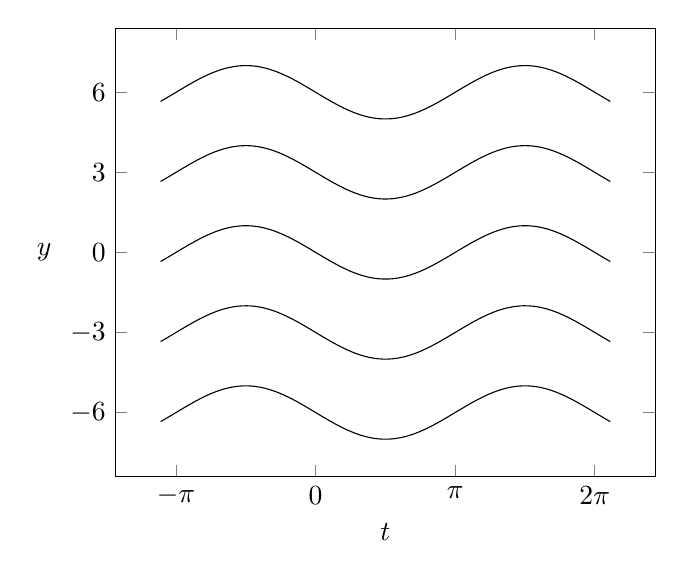
\begin{tikzpicture}
\begin{axis}[xlabel={$t$},ylabel={$y$},ylabel style={rotate=-90},xtick={-180,0,180,360},xticklabels={$-\pi$,$0$,$\pi$,$2\pi$},ytick={-6,-3,0,3,6},yticklabels={$-6$,$-3$,$0$,$3$,$6$}]
\addplot[domain=-200:380,samples=100] {6-sin(x)};
\addplot[domain=-200:380,samples=100] {3-sin(x)};
\addplot[domain=-200:380,samples=100] {-sin(x)};
\addplot[domain=-200:380,samples=100] {-3-sin(x)};
\addplot[domain=-200:380,samples=100] {-6-sin(x)};
\end{axis}
\end{tikzpicture}
\caption{مثال \حوالہ{مثال_تفرقی_اول_حل_نسل_الف} کے خط۔}
\label{شکل_مثال_تفرقی_اول_حل_نسل_الف}
\end{figure}
\انتہا{مثال}
%=========================
\ابتدا{مثال}\شناخت{مثال_تفرقی_اول_مالتھس_الف}
قوت نمائی تفاعل \عددی{y=ce^{kt}} کے تفرق سے درج ذیل تفرقی مساوات حاصل ہوتی ہے۔
\begin{align*}
y'=\frac{\dif y}{\dif t}=k ce^{kt}=ky
\end{align*}
یوں \عددی{y'=ky} تفرقی مساوات کا حل \عددی{y=ce^{kt}} ہے۔مثبت \عددی{k} کی صورت میں \عددی{y=ce^{kt}} قوت نمائی اضافے کی نمونہ کشی کرتی ہے۔جرسوموں کی تعداد اسی کلیے کے تحت بڑھتی ہے۔ وسیع رقبے کے ملک میں کم انسانی آبادی اسی کلیے کے تحت بڑھتی ہے جہاں اس کو \اصطلاح{قانون مالتُھس}\فرہنگ{قانون!مالتُھس}\فرہنگ{مالتُھس!قانون}\حاشیہب{Malthus' law}\فرہنگ{Malthus' law} کہا\حاشیہد{یہ قانون انگلستانی ماہر معاشیات طامس روبرٹ مالتُھس (1766-1834) کے نام ہے۔} جاتا ہے۔مستقل \عددی{c} کے مختلف مثبت قیمتوں اور \عددی{k=0.15} کے خطوط کو شکل \حوالہ{شکل_مثال_تفرقی_اول_مالتُھس_الف}-الف میں دکھایا گیا ہے۔ 

منفی \عددی{k} کی صورت میں \عددی{y=ce^{kt}} قوت نمائی گھٹاو مثلاً \اصطلاح{تابکاری تحلیل}\فرہنگ{تابکاری تحلیل}\فرہنگ{تحلیل!تابکاری}\حاشیہب{radioactive decay}\فرہنگ{radioactive decay} کو ظاہر کرتی ہے۔مستقل \عددی{c} کے مختلف مثبت قیمتوں اور \عددی{k=-0.15} کے خطوط کو شکل \حوالہ{شکل_مثال_تفرقی_اول_مالتُھس_الف}-ب میں دکھایا گیا ہے۔ مثال \حوالہ{مثال_اول_سادہ_تابکاری_الف} میں تابکاری تحلیل کے مسئلے پر مزید غور کیا گیا ہے۔
\begin{figure}
\centering
\begin{subfigure}{0.5\textwidth}
\centering
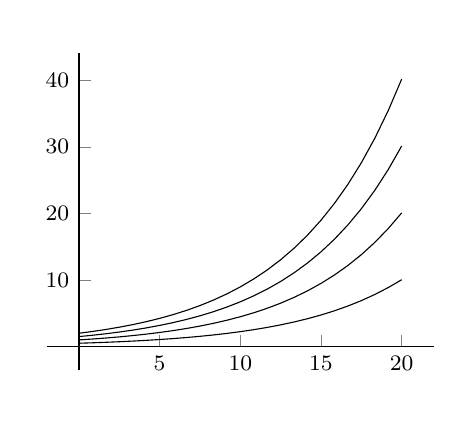
\begin{tikzpicture}
\begin{axis}[small,axis lines*=middle,ylabel style={rotate=-90},ylabel style={at={(axis description cs:0,1.05)}}]
\addplot[domain=0:20]{2*e^(0.15*x)};
\addplot[domain=0:20]{1.5*e^(0.15*x)};
\addplot[domain=0:20]{1*e^(0.15*x)};
\addplot[domain=0:20]{0.5*e^(0.15*x)};
\end{axis}
\end{tikzpicture}
\caption*{(الف) قوت نمائی اضافہ۔مساوات \عددی{y'=0.15y} کا حل۔}
\end{subfigure}%
\begin{subfigure}{0.5\textwidth}
\centering
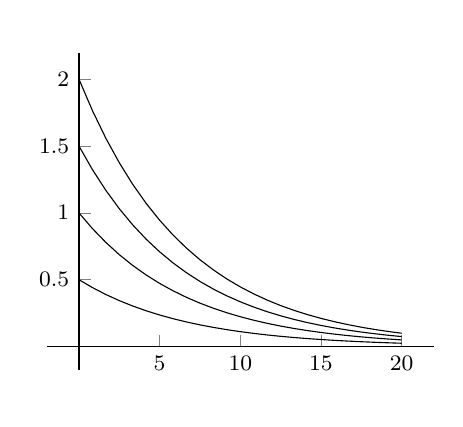
\begin{tikzpicture}
\begin{axis}[small,axis lines*=middle,ylabel style={rotate=-90},ylabel style={at={(axis description cs:0,1.05)}}]
\addplot[domain=0:20]{2*e^(-0.15*x)};
\addplot[domain=0:20]{1.5*e^(-0.15*x)};
\addplot[domain=0:20]{1*e^(-0.15*x)};
\addplot[domain=0:20]{0.5*e^(-0.15*x)};
\end{axis}
\end{tikzpicture}
\caption*{(الف) قوت نمائی گھٹاو۔مساوات \عددی{y'=-0.15y} کا حل۔}
\end{subfigure}%
\caption{قوت نمائی تفرقی مساوات کی نسل حل۔}
\label{شکل_مثال_تفرقی_اول_مالتُھس_الف}
\end{figure}
\انتہا{مثال}
%==========================

درج بالا مثالوں میں ہم نے دیکھا کہ درجہ اول سادہ تفرقی مساوات کے حل میں ایک عدد اختیاری مستقل \عددی{c} پایا جاتا ہے۔ تفرقی مساوات کا ایسا حل جس میں اختیاری مستقل \عددی{c} پایا جاتا ہو \اصطلاح{عمومی حل}\فرہنگ{عمومی حل}\فرہنگ{حل!عمومی}\حاشیہب{general solution}\فرہنگ{general solution} کہلاتا ہے۔

(بعض اوقات \عددی{c} مکمل طور اختیاری مستقل نہیں ہوتا بلکہ اس کی قیمت کو کسی وقفے پر محدود کرنا لازم ہوتا ہے۔)

ہم \اصطلاح{یکتا}\فرہنگ{یکتا!حل}\حاشیہب{unique}\فرہنگ{unique!general solution} عمومی حل حاصل کرنے کی تراکیب سیکھیں گے۔

جیومیٹریائی طور پر سادہ تفرقی مساوات کا عمومی حل لامتناہی حل کے خطوط پر مشتمل ہوتا ہے جہاں \عددی{c} کی ہر انفرادی قیمت منفرد خط دیتی ہے۔عمومی حل میں \عددی{c} کی کوئی مخصوص قیمت مثلاً \عددی{c=-3.501} یا \عددی{c=0} پر کرنے سے ہمیں \اصطلاح{جبری حل}\فرہنگ{جبری!حل}\فرہنگ{حل!جبری}\حاشیہب{particular solution}\فرہنگ{solution!particular} ملتا ہے۔جبری حل میں کوئی اختیاری مستقل نہیں پایا جاتا۔

عام طور عمومی حل قابل حصول ہوتا ہے جس میں \عددی{c} کی مخصوص قیمت پر کرتے ہوئے درکار جبری حل حاصل کیا جا سکتا ہے۔بعض اوقات تفرقی مساوات ایسا حل بھی رکھتا ہے جس کو عمومی حل سے حاصل نہیں کیا جا سکتا۔ایسے حل کو \اصطلاح{نادر}\فرہنگ{نادر!حل}\فرہنگ{حل!نادر}\حاشیہب{singular solution}\فرہنگ{singular!solution} حل کہتے ہیں۔صفحہ \حوالہصفحہ{سوال_سادہ_اول_نادر_حل_الف} پر سوال \حوالہ{سوال_سادہ_اول_نادر_حل_الف} میں نادر حل کی مثال دی گئی ہے۔

\جزوحصہء{ابتدائی قیمت سوال}
عام طور پر عمومی حل میں \اصطلاح{ابتدائی قیمتیں}\فرہنگ{ابتدائی قیمتیں}\حاشیہب{initial values}\فرہنگ{initial values} \عددی{x_0} اور \عددیء{y_0} پر کرنے سے جبری حل حاصل کیا جاتا ہے جہاں  \عددی{{y(x_0)=y_0}}  ہے۔جیومیٹریائی طور پر اس کا مطلب ہے کہ خط حل نقطہ \عددی{(x_0,y_0)} سے گزرتا ہے۔سادہ تفرقی مساوات اور مساوات کے ابتدائی قیمتوں کو \اصطلاح{ابتدائی قیمت سوال}\فرہنگ{ابتدائی قیمت سوال}\حاشیہب{initial value problem}\فرہنگ{initial value!problem} کہا جاتا ہے۔یوں صریح سادہ تفرقی مساوات کی صورت میں ابتدائی قیمت سوال درج ذیل لکھا جائے گا۔
\begin{align}
y'=f(x,y), \quad \quad y(x_0)=y_0
\end{align}

%======================
\ابتدا{مثال}
ابتدائی قیمت سوال: درج ذیل ابتدائی قیمت سوال کو حل کریں۔
\begin{align*}
y'=5y,\quad \quad y(0)=3.2
\end{align*}

حل:تفرقی مساوات کو \عددی{\tfrac{\dif y}{y}=5 \dif x} لکھتے ہوئے دونوں اطراف کا تکمل لینے سے \عددی{y=ce^{5x}} عمومی حل حاصل ہوتا ہے جس میں \عددی{x=0} پر \عددی{y=3.2} پر کرنے سے \عددی{y(0)=ce^{0}=3.2} لکھا جائے گا جس سے \عددی{c=3.2} ملتا ہے۔یوں ابتدائی قیمت سوال کا جبری حل \عددی{y=3.2e^{5x}} ہے۔
\انتہا{مثال}

%=============================
\جزوحصہء{نمونہ کشی پر مزید بحث}
نمونہ کشی کو مثال کی مدد سے بہتر سمجھا جا سکتا ہے لہٰذا ایسا ہی کرتے ہیں۔ایسا کرتے ہوئے پہلی قدم پر  مسئلے کو تفرقی مساوات کا جامہ پہنایا جائے گا۔دوسری قدم پر تفرقی مساوات کا عمومی حل حاصل کیا جائے گا۔تیسرے قدم پر ابتدائی معلومات استعمال کرتے ہوئے جبری حل حاصل کیا جائے گا۔ آخر میں چوتھا قدم حاصل جواب کی تشریح ہو گی۔ 
%=================

\ابتدا{مثال}\شناخت{مثال_اول_سادہ_تابکاری_الف}
تابکار  مادے کی موجودہ کمیت \عددی{\SI{2}{\milli\gram}} ہے۔اس کی کمیت  مستقبل میں دریافت کریں۔

طبعی معلومات: تجربے سے معلوم کیا گیا ہے کہ کسی بھی لمحے پر تابکاری تحلیل کی شرح اس لمحے پر موجود تابکار مادے کی کمیت کے راست تناسب ہے۔ 
\begin{itemize}
\item
پہلا قدم: مسئلے کو مساوات کی صورت میں لکھتے ہیں۔کمیت کو \عددی{y} سے ظاہر کرتے ہیں۔یوں کسی بھی لمحے پر تابکاری کی شرح سے مراد \عددی{y'=\tfrac{\dif y}{\dif t}} ہے جہاں \عددی{t} وقت کو ظاہر کرتا ہے۔چونکہ تابکاری سے تابکار مادے کی کمیت گھٹتی ہے لہٰذا تجربے سے حاصل معلومات کو درج ذیل تفرقی مساوات کی صورت میں لکھا جائے گا جہاں تناسبی مستقل \عددی{k} مثبت قیمت ہے۔
\begin{align}
\frac{\dif y}{\dif t}=-ky
\end{align}
مثال \حوالہ{مثال_تفرقی_اول_مالتھس_الف} میں آپ نے دیکھا کہ تفرقی مساوات میں منفی کی علامت سے تفرقی مساوات کا قوت نمائی گھٹتا ہوا حل حاصل ہوتا ہے۔چونکہ تابکاری سے تابکار مادے کی کمیت گھٹتی ہے لہٰذا درج بالا مساوات میں منفی کی علامت استعمال کی گئی ہے۔تابکار اشیاء کے مستقل \عددی{k} کی قیمتیں تجربے سے حاصل کئے جاتے ہیں مثلاً \اصطلاح{ریڈیم}\فرہنگ{ریڈیم}\حاشیہب{radium}\فرہنگ{radium} یعنی   \عددی{\ce{^{226}_{88}Ra}} کا \عددی{k=\SI{1.4e-11}{\per\second}} ہے۔

ابتدائی کمیت \عددی{\SI{2}{\milli\gram}} ہے۔ابتدائی وقت کو \عددی{t=0} لیتے  ہوئے ابتدائی معلومات \عددی{y(0)=\SI{2}{\milli\gram}} لکھی  جائے گی۔(غیر تابع متغیر وقت \عددی{t} کی بجائے  کچھ اور مثلاً \عددی{x} ہونے کی صورت میں بھی \عددی{(x_0,y_0)} یا \عددی{y(x_0)=y_0} کو ابتدائی معلومات ہی کہا جاتا ہے۔اسی طرح تابع متغیرہ \عددی{y} کی قیمت \عددی{t \ne 0} پر معلوم ہو سکتی ہے مثلاً \عددی{y(x_n)=y_n} اور ایسی صورت میں \عددی{(x_n,y_n)} ابتدائی معلومات کہلاتی ہے۔یوں دیے مسئلے سے درج ذیل ابتدائی قیمت سوال حاصل ہوتا ہے۔
\begin{align}
y'=-ky,\quad \quad y(0)=\SI{2}{\milli\gram} 
\end{align}

\item
دوسرا قدم:ابتدائی قیمت سوال کا عمومی حل درج ذیل ہے جہاں \عددی{c} اختیاری مستقل جبکہ \عددی{k} کی قیمت تابکار مادے پر منحصر ہے۔
\begin{align}
y=c^{-kt}
\end{align}
ابتدائی معلومات کے تحت \عددی{t=0} پر \عددی{y=\SI{2}{\milli\gram}} ہے جس کو درج بالا مساوات میں پر کرتے ہوئے \عددی{c=2} حاصل ہوتا ہے۔یوں درج ذیل جبری حل حاصل ہوتا ہے۔
\begin{align}\label{مساوات_سادہ_اول_جبری_تابکاری}
y=2e^{-kt}\quad \quad (k>0)
\end{align} 
جبری حل کو واپس تفرقی مساوات میں پر کرتے ہوئے ثابت کریں کہ حاصل حل درست ہے۔اسی طرح جبری حل سے ابتدائی معلومات حاصل کریں۔
\begin{align*}
\frac{\dif y}{\dif t}=-k ce^{-kt}=-ky, \quad y(0)=2e^{-0}=2
\end{align*}
%
\item
حاصل جبری حل کی تشریح:مساوات \حوالہ{مساوات_سادہ_اول_جبری_تابکاری} کو شکل \حوالہ{شکل_مثال_اول_سادہ_تابکاری_الف} میں دکھایا گیا ہے جہاں \عددی{k=2.5} لیا گیا ہے۔لمحہ \عددی{t=0} پر یہ مساوات تابکار مادے کی درست کمیت دیتا ہے۔لمحہ لامتناہی پر تابکار مادے کی کمیت \عددی{y(\infty)=2e^{-k\infty}=0} حاصل ہوتی ہے۔
\begin{figure}
\centering
\begin{tikzpicture}
\begin{axis}[small,axis lines*=middle,ylabel style={rotate=-90},ylabel style={at={(axis description cs:0,1.05)}},xlabel={$t$},ylabel={$y$}]
\addplot[domain=0:2]{2*e^(-2.5*x)};
\end{axis}
\end{tikzpicture}
\caption{مثال \حوالہ{مثال_اول_سادہ_تابکاری_الف} کی منحنی۔ تابکاری تحلیل \عددی{y=2e^{-kt}} جہاں \عددی{k=2.5} لیا گیا ہے۔}
\label{شکل_مثال_اول_سادہ_تابکاری_الف}
\end{figure} 
%
\end{itemize}
\انتہا{مثال}
%=====================

\حصہء{سوالات}
سوالات \حوالہ{سوال_سادہ_اول_تکمل_الف} تا \حوالہ{سوال_سادہ_اول_تکمل_آخر} کے جوابات بذریعہ تکمل حاصل کریں یا کسی تفاعل کی تفرق سے جواب حاصل کریں۔

\ابتدا{سوال}\شناخت{سوال_سادہ_اول_تکمل_الف}
\quad
$y'+3\sin 2\pi x=0$

جواب:\quad
  $y=\frac{3}{2\pi} \cos 2\pi x+c$
\انتہا{سوال}
%=====================
\ابتدا{سوال}\quad
$y'+xe^{-x^2}=0$

جواب:\quad
$y=\tfrac{e^{-x^2}}{2}+c$
\انتہا{سوال}
%==================
\ابتدا{سوال}\quad
$y'=4e^{-x}\cos x$

جواب:\quad
 $y=2e^{-x}(\cos x-\sin x)+c$
\انتہا{سوال}
%=======================
\ابتدا{سوال}\quad
$y'=y$

جواب:\quad
$y=ce^{x}$
\انتہا{سوال}
%======================
\ابتدا{سوال}\quad
$y'=-y$

جواب:\quad
$y=ce^{-x}$
\انتہا{سوال}
%======================
\ابتدا{سوال}\quad
$y'=2.2y$

جواب:\quad
$y=ce^{2.2x}$
\انتہا{سوال}
%======================
\ابتدا{سوال}\quad
$y'=1.5\sinh 3.2x$

جواب:\quad
$y=\tfrac{15}{32}\cosh 3.2x+c$
\انتہا{سوال}
%======================
\ابتدا{سوال}\شناخت{سوال_سادہ_اول_تکمل_آخر}
\quad
$y''=-y$

جواب:\quad
$y=c_1\cos x+c_2\sin x$
\انتہا{سوال}
%======================
سوال \حوالہ{سادہ_اول_ابتدائی_قیمت_الف} تا سوال \حوالہ{سادہ_اول_ابتدائی_قیمت_آخر} ابتدائی قیمت سوالات ہیں جن کے عمومی حل دیے گئے ہیں۔انہیں تفرقی مساوات میں پر کرتے ہوئے ثابت کریں کہ یہی عمومی جوابات ہیں۔عمومی جواب سے جبری جواب حاصل کریں۔جبری جواب کا خط کھینچیں۔

%=================================
\ابتدا{سوال}\شناخت{سادہ_اول_ابتدائی_قیمت_الف}
\quad
$y'+2y=0.8,\quad y=ce^{-2x}+0.4,\quad y(0)=1.2$

جواب:\quad
$y=0.8e^{-2x}+0.4$
\انتہا{سوال}
%==========================
\ابتدا{سوال}\quad
$y'+x+y=0,\quad y=ce^{-x}-x+1,\quad y(0)=\pi$

جواب:\quad
$y=\pi e^{-x}-e^{-x}-x+1$
\انتہا{سوال}
%==========================
\ابتدا{سوال}\quad
$y'=2x+e^{x},\quad y=e^{x}+x^2+c,\quad y(0)=1$

جواب:\quad
$y=e^{x}+x^2$
\انتہا{سوال}


%==================
\ابتدا{سوال}\quad
$y'+4xy=0,\quad y=ce^{-2x^2},\quad y(0)=2$

جواب:\quad
$y=2e^{-2x^2}$
\انتہا{سوال}
%==========
\ابتدا{سوال}\quad
$yy'=2x,\quad y^2=2x^2+c,\quad y(1)=6$

جواب:\quad
$y^2=2x^2+34$
\انتہا{سوال}
%======================
\ابتدا{سوال}\quad
$y'=y+y^2,\quad y=\tfrac{c}{e^{-x}-c},\quad y(0)=0.1$

جواب:\quad
$y=\tfrac{1}{e^{(-x+23.98)}-1}$
\انتہا{سوال}
%==================
\ابتدا{سوال}\شناخت{سادہ_اول_ابتدائی_قیمت_آخر}
\quad
$y'\tan x=y-4,\quad y=c\sin x+4,\quad y(\tfrac{\pi}{2})=0$

جواب:\quad
$y=4-4\sin x$
\انتہا{سوال}
%================
\ابتدا{سوال}\شناخت{سوال_سادہ_اول_نادر_حل_الف}
نادر حل: بعغ اوقات سادہ تفرقی مساوات کا ایسا حل بھی پایا جاتا ہے جس کو عمومی حل سے حاصل نہیں کیا جا سکتا۔ایسیے حل کو \اصطلاح{نادر حل}\فرہنگ{نادر!حل}\فرہنگ{حل!نادر}\حاشیہب{singular solution}\فرہنگ{solution!singular} کہا جاتا ہے۔مساوات \عددی{y'^2-xy'+y=0} کا عمومی حل \عددی{y=cx-c^{2}} ہے جبکہ اس کا  نادر حل \عددی{y=\tfrac{x^2}{4}} ہے۔ ان حل کا تفرق لیتے ہوئے تفرقی مساوات میں پر کرتے ہوئے ثابت کریں کہ یہ تفرقی مساوات کے حل ہیں۔
\انتہا{سوال}
%=================
سوال \حوالہ{سوال_سادہ_اول_نقشہ_کشی_الف} تا سوال \حوالہ{سوال_سادہ_اول_نقشہ_کشی_ٹ} نقشہ کشی کے سوالات ہیں۔

\ابتدا{سوال}\شناخت{سوال_سادہ_اول_نقشہ_کشی_الف}
تابکار مادے کی نصف زندگی \عددی{t_{\tfrac{1}{2}}} سے مراد وہ دورانیہ ہے جس میں تابکار مادے کی کمیت نصف ہو جاتی ہے۔مثال \حوالہ{مثال_اول_سادہ_تابکاری_الف} میں ریڈیم \ce{^{266}_{88}Ra} کی نصف زندگی دریافت کریں۔

جواب:تابکاری تحلیل کی مساوات \عددی{y=y_0e^{-kt}} میں لمحہ \عددی{t=0} پر (ابتدائی) کمیت\عددی{y_0} ہے جبکہ مستقبل میں لمحہ \عددی{t} پر کمیت \عددی{y} ہے۔ہم وہ دورانیہ جاننا چاہتے ہیں جس میں کمیت نصف رہ جائے یعنی جب \عددی{y=\tfrac{y_0}{2}} رہ جائے۔تابکاری مساوات میں \عددی{y=\tfrac{y_0}{2}} پر کرتے ہوئے \عددی{\tfrac{y_0}{2}=y_0e^{-kt}} لکھا جائے گا جس سے \عددی{t_{\tfrac{1}{2}}=\SI{4.95e10}{\second}}  یعنی \عددی{1569.6} سال  حاصل ہوتا ہے۔یوں ریڈیم کی مقدار \عددی{1569.6} سالوں میں نصف رہ جائے گی۔ 
\انتہا{سوال}
%==============================
\ابتدا{سوال}\شناخت{سوال_سادہ_اول_نقشہ_کشی_ب}
ریڈیم \اصطلاح{ہم جا}\فرہنگ{ہم جا}\حاشیہب{isotope}\فرہنگ{isotope} \ce{^{224}_{88}Ra} کی نصف زندگی تقریباً \عددی{3.6} دن ہے۔دو گرام \عددیء{(\SI{2}{\gram})} ریڈیم ہم جا کی کمیت ایک دن بعد کتنی رہ جائے گی۔دو گرام ریڈیم ہم جا کی کمیت ایک سال بعد کتنی رہ جائے گی۔

جوابات:\عددی{\SI{1.65}{\gram}}، \عددی{\SI{6e-31}{\gram}}
\انتہا{سوال}
%======================
\ابتدا{سوال}\شناخت{سوال_سادہ_اول_نقشہ_کشی_پ}
ایک جہاز کی رفتار مستقل اسراع \عددی{a} سے مسلسل بڑھ رہی ہے۔رفتار کی تبدیلی کی شرح \عددی{\tfrac{\dif v}{\dif t}} کو اسراع کہتے ہیں۔ان معلومات سے تفرقی مساوات لکھتے ہوئے لمحہ \عددی{t} پر رفتار \عددی{v} کی مساوات حاصل کریں۔اگر \عددی{t=0} پر ابتدائی رفتار \عددی{u} ہو تب \عددی{v} کی مساوات کیا ہو گی؟ 

جوابات:\عددی{v=at+c}، \عددی{v=u+at}
\انتہا{سوال}
%=========================
\ابتدا{سوال}\شناخت{سوال_سادہ_اول_نقشہ_کشی_ت}
رفتار سے مراد وقت کے ساتھ فاصلے کی تبدیلی کی شرح \عددی{\tfrac{\dif x}{\dif t}} ہے۔سوال \حوالہ{سوال_سادہ_اول_نقشہ_کشی_پ} میں رفتار کی مساوات \عددی{v=u+at} حاصل کی گئی جسے \عددی{\tfrac{\dif x}{\dif t}} کے برابر پر کرنے سے تفرقی مساوات حاصل ہوتی ہے۔لمحہ \عددی{t=0} پر ابتدائی فاصلہ \عددی{x=0} لیتے ہوئے ابتدائی قیمت سوال کو حل کرتے ہوئے  \عددی{x} کی مساوات حاصل کریں۔

جوابات:\عددی{x=ut+\tfrac{1}{2}at^2}
\انتہا{سوال}
%=========================
\ابتدا{سوال}\شناخت{سوال_سادہ_اول_نقشہ_کشی_ٹ}
آواز سے کم رفتار پر پرواز کرنے والے جہاز کی کارگزاری ہوا کے دباو پر منحصر ہوتی ہے۔ان  کی کارگزاری \عددی{\SI{10500}{\meter}} تا \عددی{\SI{12000}{\meter}} کی اونچائی پر بہترین حاصل ہوتی ہے۔آپ سے گزارش ہے کہ \عددی{\SI{10500}{\meter}} کی اونچائی پر ہوا کا دباو دریافت کریں۔طبعی معلومات:اونچائی کے ساتھ دباو میں تبدیلی کی شرح \عددی{y'} ہوا کے دباو \عددی{y} کے راست تناسب ہوتی ہے۔تقریباً \عددی{\SI{5500}{\meter}} کی اونچائی پر ہوا کا دباو سمندر کی سطح پر ہوا کے دباو \عددی{y_0} کی نصف ہوتا ہے۔

جواب:\عددی{0.27y_0}یعنی تقریباً ایک چوتھائی
\انتہا{سوال}
%===================

\حصہ{\عددی{y'=f(x,y)} کا جیومیٹریائی مطلب۔ میدان کی سمت اور ترکیب یولر۔}
درجہ اول سادہ تفرقی مساوات
\begin{align}\label{مساوات_سادہ_اول_ڈھلوان_تفاعل_الف}
y'=f(x,y)
\end{align}
سادہ معنی رکھتی ہے۔آپ جانتے ہیں کہ \عددی{y'} سے مراد \عددی{y} کی ڈھلوان ہے۔یوں مساوات \حوالہ{مساوات_سادہ_اول_ڈھلوان_تفاعل_الف} کا وہ حل جو نقطہ \عددی{(x_0,y_0)} سے گزرتا ہو کا اس نقطے پر ڈھلوان \عددی{y'(x_0)} ہو گا کو درج بالا مساوات کے تحت اس نقطے پر \عددی{f} کی قیمت کے برابر ہو گا۔
\begin{align*}
y'(x_0)=f(x_0,y_0)
\end{align*}
اس حقیقت کو استعمال کرتے ہوئے ہم مساوات \حوالہ{مساوات_سادہ_اول_ڈھلوان_تفاعل_الف} کو حل کرنے کے  \اصطلاح{ترسیمی}\فرہنگ{ترسیمی}\حاشیہب{graphical}\فرہنگ{graphical} یا \اصطلاح{اعدادی}\فرہنگ{اعدادی}\حاشیہب{numerical}\فرہنگ{numerical} طریقے دریافت کر سکتے ہیں۔تفرقی مساوات کو حل کرنے کے ترسیمی اور اعدادی طریقے اس لئے بھی اہم ہیں کہ کئی تفرقی مساوات کا کوئی \اصطلاح{تحلیلی}\فرہنگ{تحلیلی}\حاشیہب{analytic}\فرہنگ{analytic} حل نہیں پایا جاتا جبکہ ہر قسم کے تفرقی مساوات کا ترسیمی اور اعدادی حل حاصل کرنا ممکن ہے۔   

\جزوحصہء{میدان کی سمت: ترسیمی طریقہ}
ہم \عددی{xy} سطح پر جگہ جگہ مساوات \حوالہ{مساوات_سادہ_اول_ڈھلوان_تفاعل_الف} سے حاصل ڈھلوان کی چھوٹی لمبائی کی سیدھی لکیریں کھینچ سکتے ہیں۔ہر نقطے پر ایسی لکیر اس نقطے پر میدان کی سمت دیتی ہے۔اس \اصطلاح{میدانِ سمت}\فرہنگ{میدانِ!سمت}\حاشیہب{direction field}\فرہنگ{direction field} یا  \اصطلاح{میدانِ ڈھال}\فرہنگ{میدان!ڈھال}\فرہنگ{ڈھال!میدان}\حاشیہب{slope field}\فرہنگ{field!slope}\فرہنگ{slope!field} میں تفرقی مساوات کا  \اصطلاح{منحنی حل}\فرہنگ{منحنی حل}\حاشیہب{solution curve}\فرہنگ{solution curve} کھینچا جا سکتا ہے۔

منحنی حل کو کھینچنے کی ترکیب کچھ یوں ہے۔کسی بھی نقطے پر ڈھلوان کی سمت میں چھوٹی لکیر کھینچیں۔اس لکیر کو آہستہ آہستہ یوں موڑیں کہ لکیر کے اختتامی نقطے پر لکیر کی ڈھلوان عین اس نقطے کی ڈھلوان برابر ہو۔اسی طرح آگے بڑھتے رہیں۔ڈھال میدان میں نقطے جتنے قریب قریب ہوں تفرقی مساوات کا منحنی حل اتنا درست ہو گا۔

شکل \حوالہ{شکل_اول_سادہ_منحنی_حل_الف} میں 
\begin{align}\label{مساوات_اول_سادہ_ب}
y'=x-y
\end{align}
کا ڈھال میدان دکھایا گیا ہے۔ساتھ ہی ساتھ چند منحنی حل بھی دکھائے گئے ہیں۔
\begin{figure}
\centering
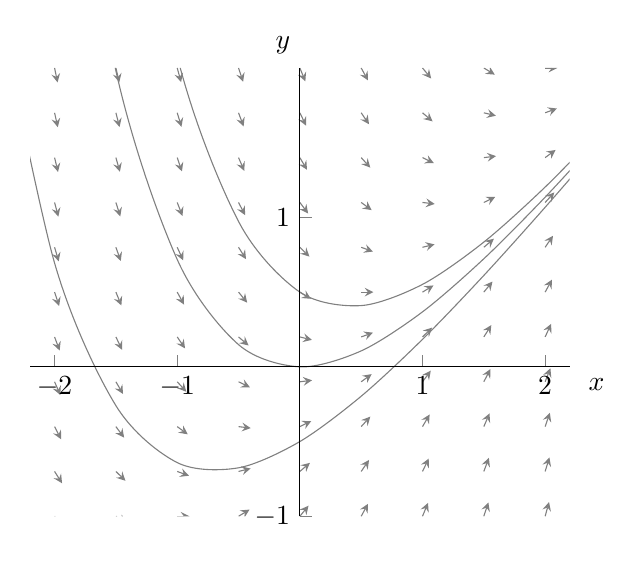
\begin{tikzpicture}
\def\length{sqrt(1+(x-y)^2)}
\begin{axis}[ axis lines*=middle,view={0}{90}, xlabel={$x$},ylabel={$y$},ylabel style={rotate=-90},ylabel style={at={(axis description cs:0.5,1.05)}},xmin=-2.2, xmax=2.2, ymin=-1, ymax=2,domain=-2.5:2.5, y domain=-1:2, samples=11,ytick={-1,0,1},yticklabels={$-1$,$0$,$1$},xlabel style={at={(axis description cs:1.05,0.33)}}]
\addplot3 [gray, quiver={u={1/\length}, v={(x-y)/\length}, scale arrows=0.1},-stealth] (x,y,0); %differential equation
\addplot [gray,smooth]{x-1+e^(-x)}; %actual curve
\addplot [gray,smooth]{x-1+0.5*e^(-x)}; %actual curve
\addplot [gray,smooth]{x-1+1.5*e^(-x)}; %actual curve
\end{axis}
\end{tikzpicture}
\caption{درجہ اول سادہ تفرقی مساوات \عددی{y'=x-y} کا ڈھال میدان اور منحنی حل۔}
\label{شکل_اول_سادہ_منحنی_حل_الف}
\end{figure}

آئیں اب اعدادی طریقہ سیکھیں۔سادہ ترین اعدادی طریقہ \اصطلاح{ترکیب یولر} کہلاتا ہے۔پہلے اسی پر بحث کرتے ہیں۔

\جزوحصہء{یولر کی اعدادی ترکیب}
درجہ اول تفرقی مساوات \عددی{y'=f(x,y)} اور ابتدائی معلومات \عددی{y(x_0)=y_0} کو استعمال کرتے ہوئے  \اصطلاح{ترکیب یولر}\فرہنگ{یولر!ترکیب}\حاشیہب{Euler's method}\فرہنگ{Euler's method} ہم فاصلہ نقطوں \عددی{x_0}، \عددی{x_1=x_0+h}، \عددی{x_2=x_0+2h}، \عددی{\cdots} پر تقریباً درست قیمتیں دیتا ہے یعنی
\begin{align*}
y_1&=y_0+hf(x_0,y_0)\\
y_2&=y_1+hf(x_1,y_1)\\
y_3&=y_2+hf(x_2,y_2)
\end{align*}
یا
\begin{align}\label{مساوات_سادہ_اول_یولر_مساوات}
y_n=y_{n-1}+hf(x_{n-1},y_{n-1})
\end{align}
\عددی{h} کو قدم کہتے ہیں۔شکل \حوالہ{شکل_سادہ_اول_ترکیب_یولر_پہلا_قدم}-الف میں \عددی{y_1} کا حصول دکھایا گیا ہے  جہاں ابتدائی نقطہ \عددی{y_0} اور ترکیب یولر سے حاصل کردہ \عددی{y_1} کو چھوٹے دائروں سے ظاہر کیا گیا ہے۔ شکل-ب میں \عددی{h} کی قیمت کم کرنے کا اثر دکھایا گیا ہے۔آپ دیکھ سکتے ہیں کہ چھوٹا قدم لینے سے اصل حل \عددی{y(x_1)} اور یولر سے حاصل \عددی{y_1} میں فرق (غلطی) کم ہو جاتا ہے۔یوں قدم کو چھوٹا سے چھوٹا کرتے ہوئے زیادہ سے زیادہ درست حل دریافت کیا جا سکتا ہے۔
\begin{figure}
\centering
\begin{subfigure}{0.5\textwidth}
\centering
\begin{tikzpicture}
\begin{axis}[small,axis lines*=middle,xmin=0,xmax=4,ymin=0,xtick={0,1,2.5},xticklabels={$0$,$x_0$,$x_1$},ytick={0,2.718,6.7957,12.182},yticklabels={$0$,$y_0$,$y_1$,$y(x_1)$},xlabel={$x$},ylabel={$y$},ylabel style={rotate=-90},ylabel style={at={(axis description cs: 0,1.05)}},xlabel style={at={(axis description cs:1.05,0)}}]
\addplot[domain=1:3]{e^x}node[left]{\RL{حل منحنی}};
\addplot[domain=1:2.5]{e^(1)*x};
\addplot[dashed] plot coordinates {(0,e) (1,e)};
\addplot[dashed] plot coordinates {(0,e*2.5) (2.5,e*2.5)};
\addplot[dashed] plot coordinates {(1,0) (1,e)};
\addplot[dashed] plot coordinates {(2.5,0) (2.5,e)};
\addplot[dashed] plot coordinates {(0,e^2.5) (2.5,e^2.5)};
\addplot[gray,stealth-stealth] plot coordinates {(1,e) (2.5,e)}node[pos=0.5,fill=white]{$h$};
\addplot[gray,stealth-stealth] plot coordinates {(2.5,e) (2.5,e*2.5)}node[pos=0.5,right]{$hf(x_0,y_0)$};
\addplot[gray,stealth-stealth] plot coordinates {(2.5,e*2.5) (2.5,e^2.5)}node[pos=0.5,right]{غلطی};
\addplot[] plot coordinates {(1,e)}node[ocirc]{};
\addplot[] plot coordinates {(2.5,e*2.5)}node[ocirc]{};
\end{axis}
\end{tikzpicture}
\caption*{(الف)}
\end{subfigure}%
\begin{subfigure}{0.5\textwidth}
\centering
\begin{tikzpicture}
\pgfmathsetmacro{\xa}{2}
\pgfmathsetmacro{\ya}{e*\xa}
\pgfmathsetmacro{\yb}{e^\xa}
\begin{axis}[small,axis lines*=middle,xmin=0,xmax=4,ymin=0,xtick={0,1,\xa},xticklabels={$0$,$x_0$,$x_1$},ytick={0,2.718,\ya,\yb},yticklabels={$0$,$y_0$,$y_1$,$y(x_1)$},xlabel={$x$},ylabel={$y$},ylabel style={rotate=-90},ylabel style={at={(axis description cs: 0,1.05)}},xlabel style={at={(axis description cs:1.05,0)}}]
\addplot[domain=1:3]{e^x}node[left]{\RL{حل منحنی}};
\addplot[domain=1:\xa]{e^(1)*x};
\addplot[dashed] plot coordinates {(0,e) (1,e)};
\addplot[dashed] plot coordinates {(0,e*\xa) (\xa,e*\xa)};
\addplot[dashed] plot coordinates {(1,0) (1,e)};
\addplot[dashed] plot coordinates {(\xa,0) (\xa,e)};
\addplot[dashed] plot coordinates {(0,e^\xa) (\xa,e^\xa)};
\addplot[gray,stealth-stealth] plot coordinates {(1,e) (\xa,e)}node[pos=0.5,below]{$h$};
\addplot[gray,stealth-stealth] plot coordinates {(\xa,e) (\xa,e*\xa)};
\addplot[gray,stealth-stealth] plot coordinates {(\xa,e*\xa) (\xa,e^\xa)};
\addplot[] plot coordinates {(1,e)}node[ocirc]{};
\addplot[] plot coordinates {(\xa,e*\xa)}node[ocirc]{};
\end{axis}
\end{tikzpicture}
\caption*{(ب)}
\end{subfigure}%
\caption{ترکیب یولر کا پہلا قدم۔}
\label{شکل_سادہ_اول_ترکیب_یولر_پہلا_قدم}
\end{figure}

مساوات \حوالہ{مساوات_اول_سادہ_ب} کا عمومی حل \عددی{y=ce^{-x}+x-1} ہے جس سے  نقطہ \عددی{(0,0)} سے گزرتا حل \عددی{y=e^{-x}+x-1} ملتا ہے۔اس طرح کے حل ہم جلد حاصل کر پائیں گے۔اس وقت صرف اتنا ضروری ہے کہ  آپ دیے گئے حل کو تفرقی مساوات میں پر کرتے ہوئے ثابت کر سکیں کہ یہی درست حل ہے۔

جدول \حوالہ{جدول_اول_سادہ_یولر_الف} میں قدم \عددی{h=0.1} لیتے ہوئے نقطہ \عددی{(0,0)} سے گزرتا ہوا  مساوات \حوالہ{مساوات_اول_سادہ_ب} کا ترکیب یولر (مساوات \حوالہ{مساوات_سادہ_اول_یولر_مساوات}) سے حل حاصل کیا گیا ہے۔آئیں اس جدول کو حاصل کریں۔

ابتدائی نقطہ \عددی{(x_0,y_0)=(0,0)} ہے جس کا اندراج جدول \حوالہ{جدول_اول_سادہ_یولر_الف} کے پہلے صف میں کیا گیا ہے۔ان قیمتوں کو استعمال کرتے ہوئے \عددی{(x_1,y_1)} حاصل کرتے ہیں۔
\begin{align*}
x_1&=x_0+h=0+0.1=0.1\\
y_1&=y_0+h f(x_0,y_0)=y_0+h(x_0-y_0)=0+0.1(0-0)=0
\end{align*}
جدول \حوالہ{جدول_اول_سادہ_یولر_الف} کے دوسرے صف میں ان قیمتوں کا اندراج کیا گیا ہے جن سے \عددی{(x_2,y_2)} حاصل کرتے ہیں۔
\begin{align*}
x_2&=x_1+h=0.1+0.1=0.2\\
y_2&=y_1+h f(x_1,y_1)=y_1+h(x_1-y_1)=0+0.1(0.1-0)=0.01
\end{align*}
یہ قیمتیں بھی جدول میں درج ہیں۔اسی طرح \عددی{(x_3,y_3)} حاصل کرتے ہوئے جدول میں درج کئے گئے ہیں۔
\begin{align*}
x_3&=x_2+h=0.2+0.1=0.3\\
y_3&=y_2+h f(x_2,y_2)=y_2+h(x_2-y_2)=0.01+0.1(0.2-0.01)=0.029
\end{align*}
جدول کی آخری صف حاصل کرتے ہیں۔
\begin{align*}
x_4&=x_3+h=0.3+0.1=0.4\\
y_4&=y_3+h f(x_3,y_3)=y_3+h(x_3-y_3)=0.029+0.1(0.3-0.029)=0.0561
\end{align*}
شکل \حوالہ{شکل_سادہ_اول_یولر_اصل_موازنہ}-الف میں ترکیب یولر سے حاصل حل اور ریاضیاتی حل \عددی{y(x)} کا موازنہ کیا گیا ہے۔شکل-الف میں یولر حل سے حاصل نقطوں کو سیدھی لکیروں سے ملاتے ہوئے مسلسل حل حاصل کیا جا سکتا ہے جسے شکل-ب میں \عددی{y_n} سے ظاہر کیا گیا ہے۔شکل-ب میں \عددی{y(x)} بھی دکھایا گیا ہے۔ساتھ ہی ساتھ \عددی{h=0.05} استعمال کرتے ہوئے حاصل یولر حل کو بھی دکھایا گیا ہے جو \عددی{y(x)} اور \عددی{y_n} کے بیچ میں پایا جاتا ہے۔آپ دیکھ سکتے ہیں کہ \عددی{h} کی قیمت کم کرنے سے زیادہ درست جواب حاصل ہوتا ہے۔ 
\begin{table}
\caption{ترکیب یولر۔}
\label{جدول_اول_سادہ_یولر_الف}
\centering
\begin{tabular}{lllll}
$n$&$x_n$&$y_n$&$y(x)$&\text{غلطی}\\
\hline
0&0&0&0&0\\
1&0.1&0.0&0.00484&0.00484\\
2&0.2&0.01&0.01873&0.00873\\
3&0.3&0.029&0.04082&0.01182\\
4&0.4&0.0561&0.07032&0.01422
\end{tabular}
\end{table}
%
\begin{figure}
\centering
\begin{subfigure}{0.5\textwidth}
\centering
\begin{tikzpicture}
\begin{axis}[small,axis lines*=middle,scaled x ticks=false,scaled y ticks=false,xlabel={$x$},ylabel={$y$},xlabel style={at={(axis description cs:1.05,0)}},ylabel style={rotate=-90},ylabel style={at={(axis description cs:0,1.05)}},xmin=0,ymin=0,ymax=0.07,ytick={0,0.02,0.04,0.06},yticklabels={$0$,$0.02$,$0.04$,$0.06$}]
\addplot[domain=0:0.4]{e^(-x)+x-1}node[pos=0.75,pin=135:{$y(x)$}]{};
\addplot[] plot coordinates {(0,0)}node[circ]{};
\addplot[] plot coordinates {(0.1,0)}node[circ]{};
\addplot[] plot coordinates {(0.2,0.01)}node[circ]{};
\addplot[] plot coordinates {(0.3,0.029)}node[circ]{};
\addplot[] plot coordinates {(0.4,0.0561)}node[circ]{};
\end{axis}
\end{tikzpicture}
\caption*{(الف)}
\end{subfigure}%
\begin{subfigure}{0.5\textwidth}
\centering
\includegraphics[]{figODEeuler}
\caption*{(ب)}
\end{subfigure}%
\caption{ترکیب یولر سے حاصل حل کا ریاضیاتی حل کے ساتھ موازنہ کیا گیا ہے۔}
\label{شکل_سادہ_اول_یولر_اصل_موازنہ}
\end{figure}

%====================
سوال \حوالہ{سوال_سادہ_اول_میدان_ڈھال_الف} تا سوال \حوالہ{سوال_سادہ_اول_میدان_ڈھال_ت} کے میدان ڈھال کو قلم و کاغذ سے کھینچتے ہوئے دیے ابتدائی نقطوں سے گزرتے منحنی حل حاصل کریں۔چند ڈھال میدان شکل \حوالہ{شکل_سوال_سادہ_اول_میدان_ڈھال_الف} اور شکل \حوالہ{شکل_سوال_سادہ_اول_میدان_ڈھال_پ} میں دیے گئے ہیں۔

%==========================

\حصہء{سوالات}
\ابتدا{سوال}\شناخت{سوال_سادہ_اول_میدان_ڈھال_الف}\quad \quad
$y'=1+y^2,\quad (\tfrac{\pi}{4},1)$
\انتہا{سوال}
%====================
\ابتدا{سوال}\شناخت{سوال_سادہ_اول_میدان_ڈھال_ب}\quad \quad
$y'=1-y^2,\quad (0,0)$
\انتہا{سوال}
%====================
\ابتدا{سوال}\شناخت{سوال_سادہ_اول_میدان_ڈھال_بب}\quad \quad
$yy'+8x=0,\quad (1,1)$
\انتہا{سوال}
%====================
\ابتدا{سوال}\شناخت{سوال_سادہ_اول_میدان_ڈھال_پ} \quad \quad
$y'=y-y^2,\quad (1,0)$
\انتہا{سوال}
%====================
\ابتدا{سوال} \شناخت{سوال_سادہ_اول_میدان_ڈھال_پپ}\quad \quad
$y'=x+\tfrac{1}{y},\quad (0,1)$
\انتہا{سوال}
%====================
\ابتدا{سوال} \شناخت{سوال_سادہ_اول_میدان_ڈھال_پپپ}\quad \quad
$y'=\sin^2 x,\quad (0,1)$
\انتہا{سوال}
%====================
\ابتدا{سوال}\شناخت{سوال_سادہ_اول_میدان_ڈھال_ت} \quad \quad
$y'=\sin^2 y,\quad (0,0)$
\انتہا{سوال}
%==================================
\begin{figure}
\centering
\begin{subfigure}{0.5\textwidth}
\centering
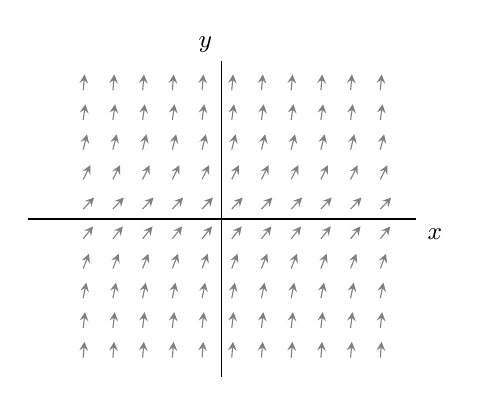
\begin{tikzpicture}
\def\length{sqrt(1+(1+y^2)^2)}
\begin{axis}[small, axis equal,axis lines*=middle,view={0}{90}, xlabel={$x$},ylabel={$y$},ylabel style={rotate=-90},ylabel style={at={(axis description cs:0.5,1.05)}},xmin=-4,xmax=4,ymin=-4,ymax=4,domain=-3.5:4, y domain=-3.5:4, samples=11,xlabel style={at={(axis description cs:1.05,0.5)}},xtick=\empty,ytick=\empty]
\addplot3 [gray, quiver={u={1/\length}, v={(1+y^2)/\length}, scale arrows=0.4,},-stealth] (x,y,0); %differential equation
\end{axis}
\end{tikzpicture}%
\caption*{(الف) \quad $y'=1+y^2$}
\end{subfigure}%
\begin{subfigure}{0.5\textwidth}
\centering
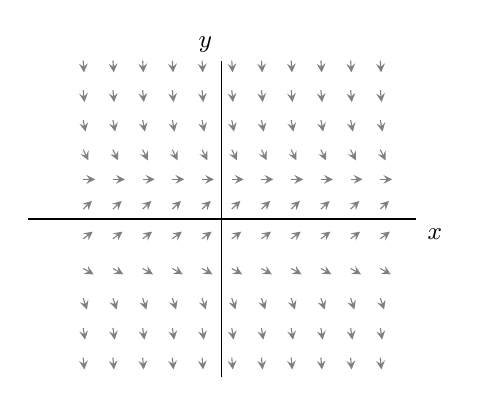
\begin{tikzpicture}
\def\length{sqrt(1+(1-y^2)^2)}
\begin{axis}[small, axis equal,axis lines*=middle,view={0}{90}, xlabel={$x$},ylabel={$y$},ylabel style={rotate=-90},ylabel style={at={(axis description cs:0.5,1.05)}},xmin=-4,xmax=4,ymin=-4,ymax=4,domain=-3.5:4, y domain=-3.5:4, samples=11,xlabel style={at={(axis description cs:1.05,0.5)}},xtick=\empty,ytick=\empty]
\addplot3 [gray, quiver={u={1/\length}, v={(1-y^2)/\length}, scale arrows=0.3},-stealth] (x,y,0); %differential equation
\end{axis}
\end{tikzpicture}%
\caption*{(ب) \quad $y'=1-y^2$}
\end{subfigure}%
\caption{سوال \حوالہ{سوال_سادہ_اول_میدان_ڈھال_الف} اور سوال \حوالہ{سوال_سادہ_اول_میدان_ڈھال_ب} کے ڈھال میدان۔}
\label{شکل_سوال_سادہ_اول_میدان_ڈھال_الف}
\end{figure}
%=============================
\begin{figure}
\centering
\begin{subfigure}{0.5\textwidth}
\centering
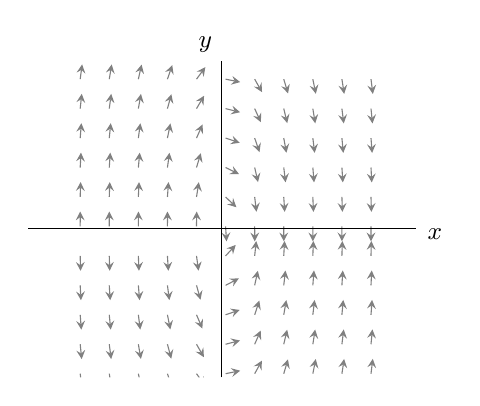
\begin{tikzpicture}
\def\length{sqrt(1+(-8*x/y)^2)}
\begin{axis}[small, axis equal,axis lines*=middle,view={0}{90}, xlabel={$x$},ylabel={$y$},ylabel style={rotate=-90},ylabel style={at={(axis description cs:0.5,1.05)}},xmin=-4,xmax=4,ymin=-4,ymax=4.5,domain=-3.8:4, y domain=-3.9:4, samples=11,xlabel style={at={(axis description cs:1.05,0.5)}},xtick=\empty,ytick=\empty]
\addplot3 [gray, quiver={u={1/\length}, v={(-8*x/y)/\length}, scale arrows=0.4,},-stealth] (x,y,0); %differential equation
\end{axis}
\end{tikzpicture}%
\caption*{(الف) \quad $y'=-\tfrac{8x}{y}$}
\end{subfigure}%
\begin{subfigure}{0.5\textwidth}
\centering
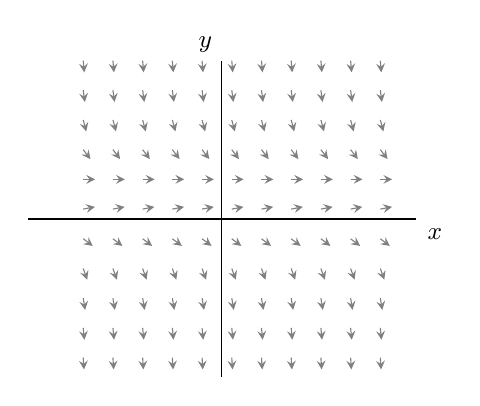
\begin{tikzpicture}
\def\length{sqrt(1+(y-y^2)^2)}
\begin{axis}[small, axis equal,axis lines*=middle,view={0}{90}, xlabel={$x$},ylabel={$y$},ylabel style={rotate=-90},ylabel style={at={(axis description cs:0.5,1.05)}},xmin=-4,xmax=4,ymin=-4,ymax=4,domain=-3.5:4, y domain=-3.5:4, samples=11,xlabel style={at={(axis description cs:1.05,0.5)}},xtick=\empty,ytick=\empty]
\addplot3 [gray, quiver={u={1/\length}, v={(y-y^2)/\length}, scale arrows=0.3},-stealth] (x,y,0); %differential equation
\end{axis}
\end{tikzpicture}%
\caption*{(ب) \quad $y'=y-y^2$}
\end{subfigure}%
\caption{سوال \حوالہ{سوال_سادہ_اول_میدان_ڈھال_بب} اور سوال \حوالہ{سوال_سادہ_اول_میدان_ڈھال_پ} کے ڈھال میدان۔}
\label{شکل_سوال_سادہ_اول_میدان_ڈھال_پ}
\end{figure}


%====================
ڈھال میدان کے استعمال سے تفرقی مساوات کے تمام حل سامنے آ جاتے ہیں۔بعض اوقات تفرقی مساوات کا تحلیلی حل حاصل کرنا ممکن ہی نہیں ہوتا۔درج ذیل دو سوالات میں ڈھال میدان سے اخذ حل اور دیے گئے تحلیلی حل کا موازنہ کرتے ہوئے ڈھال میدان سے حاصل حل کی درستگی کا اندازہ لگایا جا سکتا ہے۔

%=================
\ابتدا{سوال}\quad \quad
$y'=\sin x,\quad (\tfrac{\pi}{2},0),\quad y=-\cos x$
\انتہا{سوال}
%=====================
\ابتدا{سوال}\quad \quad
$y'=3x^2,\quad (0,0),\quad y=x^3$
\انتہا{سوال}
%=====================

%=============================
\ابتدا{سوال}
سوال \حوالہ{سوال_سادہ_اول_میدان_ڈھال_ب}، سوال \حوالہ{سوال_سادہ_اول_میدان_ڈھال_پ} اور سوال \حوالہ{سوال_سادہ_اول_میدان_ڈھال_ت} میں بے قابو متغیرہ \عددی{x} صریحاً  ظاہر نہیں کیا گیا ہے۔ایسی مساوات جن میں بے قابو متغیرہ کو صریحاً ظاہر نہ کیا جائے \اصطلاح{خود مختار}\فرہنگ{خود مختار!سادہ تفرقی مساوات}\فرہنگ{تفرقی!خود مختار}\حاشیہب{autonomous ordinary differential equations}\فرہنگ{autonomous!differential equation}\فرہنگ{differential!autonomous} سادہ تفرقی مساوات کہلاتے ہیں۔ خود مختار سادہ تفرقی مساوات کے  \اصطلاح{ہم میلان}\فرہنگ{ہم میلان}\حاشیہب{isoclines}\فرہنگ{isoclines} حل \عددی{f(x,y)=c} کی شکل و صورت کیا ہو گی؟

جواب:چونکہ \عددی{y'} کا دارومدار \عددی{x} پر نہیں ہے لہٰذا \عددی{x} تبدیل کرنے سے \عددی{y} کا میلان تبدیل نہیں ہو گا اور \عددی{f(x,y)=c} افقی محور کے متوازی خط ہوں گے۔ 
\انتہا{سوال}
%================

ایک جسم \عددی{y} محدد پر حرکت کرتی ہے۔لمحہ \عددی{t} پر نقطہ \عددی{y=0} سے جسم کا فاصلہ \عددی{y(t)} ہے۔سوالات \حوالہ{سوال_سادہ-اول_رفتار_الف} تا سوال \حوالہ{سوال_سادہ-اول_رفتار_پ} میں دئے شرائط کے مطابق جسم کی رفتار کی نمونہ کشی کریں۔ریاضی نمونے کی ڈھال میدان بناتے ہوئے  دیے گئے ابتدائی معلومات پر پورا اترتا منحنی خط کھینچیں۔ 

%=====================
\ابتدا{سوال}\شناخت{سوال_سادہ-اول_رفتار_الف}
جسم کی رفتار ضرب فاصلہ \عددی{y(t)} مستقل ہے جو \عددی{4} کے برابر ہے جبکہ \عددی{y(0)=4} کے برابر ہے۔

جوابات:\عددی{yy'=4}، \عددی{y=8t+16}
\انتہا{سوال}
%======================
\ابتدا{سوال}
رفتار ضرب وقت فاصلے کے برابر ہے۔لمحہ \عددی{t=1} پر فاصلہ \عددی{y(1)=2} ہے۔

جوابات:\عددی{y=y' t}، \عددی{y=2t}
\انتہا{سوال}
%=====================
\ابتدا{سوال}\شناخت{سوال_سادہ-اول_رفتار_پ}
مربع رفتار منفی مربع فاصلہ اکائی کے برابر ہے۔ابتدائی فاصلہ اکائی کے برابر ہے۔

جوابات:\عددی{y'=\sqrt{1+y^2}}، \عددی{\sinh^{-1}y=t+\sinh^{-1}1}
\انتہا{سوال}
%======================
\ابتدا{سوال}
ہوائی جہاز سے چھلانگ لگا کر زمین تک خیریت سے بذریعہ چھتری  اترا جا سکتا ہے۔گرتے ہوئے شخص پر آپس میں الٹ، دو عدد قوتیں عمل کرتی ہیں۔پہلی قوت زمینی کشش \عددی{F_1=mg} ہے جہاں \عددی{m} اس شخص کی کمیت اور \عددی{g=\SI{9.8}{\meter\per\second\squared}} ثقلی اسراع ہے۔یہ قوت انسان کو زمین کی طرف اسراع دیتی ہے۔دوسری قوت چھتری پر ہوا کے رگڑ سے پیدا قوت ہے جو اس شخص کی رفتار کو بڑھنے سے روکتی ہے۔چھتری پر ہوا کے رگڑ سے رفتار کے مربع کے متناسب قوت \عددی{F_2=cv^2} پیدا ہوتی ہے۔نیوٹن کی مساوات حرکت کہتی ہے کہ کسی بھی جسم پر قوت، اس جسم کی کمیت ضرب اسراع کے برابر ہوتی ہے۔چھتری سے زمین پر اترتے شخص کی نمونہ کشی کرتے ہوئے رفتار \عددی{v} کی سادہ تفرقی مساوات حاصل کریں۔کمیت کو \عددی{m=1} اور مستقل کو \عددی{c=1} لیتے ہوئے ڈھال میدان کھینچیں۔ تصور کریں کہ چھتری اس لمحہ کھلتی ہے جب شخص کی رفتار \عددی{v=\SI{15}{\meter\per\second}} ہو۔ایسی صورت میں منحنی حل حاصل کریں۔اس شخص کی اختتامی رفتار کیا ہو گی؟ کیا چھتری پر قوت رفتار کے راست متناسب ہونے کی صورت میں بھی چھتری کے ذریعہ ہوائی جہاز سے زمین تک خیریت سے چھلانگ لگائی جا سکتی ہے؟

جوابات:\عددی{mg-cv^2=m\tfrac{\dif v}{\dif t}}؛ گرنے کی رفتار اس قیمت پر رہتی ہے جہاں نیچے جانب قوت \عددی{mg} اور چھتری کی رکاوٹی اوپر جانب قوت \عددی{cv^2} برابر ہوں۔ایسی صورت میں گرتے شخص کی رفتار تبدیل نہیں ہوتی یعنی \عددی{y'=0} ہوتا ہے۔تفرقی مساوات میں \عددی{y'=0} پر کرتے اور \عددی{m=c=1} لیتے ہوئے اختتامی رفتار \عددی{v(t=\infty)=\SI{3.13}{\meter\per\second}} حاصل ہوتی ہے۔
\انتہا{سوال}
%=====================
\ابتدا{سوال}\شناخت{سوال_سادہ_اول_گول_دائرہ_ڈھال_میدان}
گول دائرے کی مساوات \عددی{x^2+y^2=r^2} ہے۔رداس \عددی{r} کو مستقل تصور کرتے ہوئے دائرے کی مساوات کا تفرق لیتے ہوئے  ڈھال میدان کی تفرقی مساوات حاصل کریں۔ڈھال میدان کھینچیں۔کیا آپ ڈھال میدان کو دیکھ کر کہہ سکتے ہیں کہ منحنی حل گول دائرے ہیں؟ اسی طرح \عددی{x^2+9y^2=c} کا تفرق لیتے ہوئے سادہ تفرقی مساوات حاصل کریں۔تفرقی مساوات کی ڈھال میدان کھینچیں۔ کیا ڈھال میدان کو دیکھ کر کہا جا سکتا ہے کہ منحنی حل بیضوی ہو گا؟

جوابات:\عددی{y'=-\tfrac{x}{y}}، \عددی{y'=-\tfrac{x}{9y}}
\begin{figure}
\centering
\begin{subfigure}{0.5\textwidth}
\centering
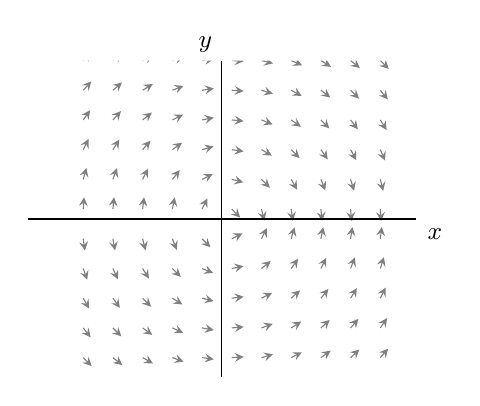
\begin{tikzpicture}
\def\length{sqrt(1+(x/y)^2)}
\begin{axis}[small, axis equal,axis lines*=middle,view={0}{90}, xlabel={$x$},ylabel={$y$},ylabel style={rotate=-90},ylabel style={at={(axis description cs:0.5,1.05)}},xmin=-4,xmax=4,ymin=-4,ymax=4,domain=-3.5:4, y domain=-3.5:4, samples=11,xlabel style={at={(axis description cs:1.05,0.5)}},xtick=\empty,ytick=\empty]
\addplot3 [gray, quiver={u={1/\length}, v={(-x/y)/\length}, scale arrows=0.3,},-stealth] (x,y,0); %differential equation
\end{axis}
\end{tikzpicture}%
\caption*{(الف) تفرقی مساوات \عددی{y'=-\tfrac{x}{y}} کی ڈھال میدان۔}
\end{subfigure}%
\begin{subfigure}{0.5\textwidth}
\centering
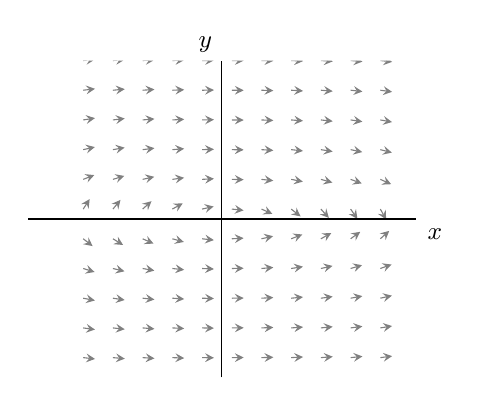
\begin{tikzpicture}
\def\length{sqrt(1+(x/(9*y))^2)}
\begin{axis}[small, axis equal,axis lines*=middle,view={0}{90}, xlabel={$x$},ylabel={$y$},ylabel style={rotate=-90},ylabel style={at={(axis description cs:0.5,1.05)}},xmin=-4,xmax=4,ymin=-4,ymax=4,domain=-3.5:4, y domain=-3.5:4, samples=11,xlabel style={at={(axis description cs:1.05,0.5)}},xtick=\empty,ytick=\empty]
\addplot3 [gray, quiver={u={1/\length}, v={(-x/(9*y))/\length}, scale arrows=0.3},-stealth] (x,y,0); %differential equation
\end{axis}
\end{tikzpicture}%
\caption*{(ب) تفرقی مساوات \عددی{y'=-\tfrac{x}{9y}} کی ڈھال میدان۔}
\end{subfigure}%
\caption{سوال \حوالہ{سوال_سادہ_اول_گول_دائرہ_ڈھال_میدان} کی ڈھال میدان۔}
\label{شکل_سوال_سادہ_اول_گول_دائرہ_ڈھال_میدان}
\end{figure}
\انتہا{سوال}
%===============================
سوال \حوالہ{سوال_سادہ_اول_یولر_الف} تا سوال \حوالہ{سوال_سادہ_اول_یولر_ت} کو ترکیب یولر سے حل کریں۔کل پانچ ہم فاصلہ نقطوں پر حل حاصل کریں۔ایک ہی کارتیسی محدد پر حاصل \عددی{y_1} تا \عددی{y_{5}} اور سوال میں دئے گئے حل \عددی{y(x)} کا خط کھینچیں۔
%=====================
\ابتدا{سوال}\شناخت{سوال_سادہ_اول_یولر_الف}
\begin{align*}
y'=-y,\quad y(0)=1,\quad h=0.1,\quad y(x)=e^{-x}
\end{align*}

جوابات: \عددی{y_1=0.9}، \عددی{y_2=0.81}، \عددی{y_3=0.729}، \عددی{y_4=0.6561}، \عددی{y_5=0.59049}
\انتہا{سوال}
%======================
\ابتدا{سوال}\شناخت{سوال_سادہ_اول_یولر_ب}
\begin{align*}
y'=-y,\quad y(0)=1,\quad h=0.01,\quad y(x)=e^{-x}
\end{align*}

جوابات: \عددی{y_1=0.99}، \عددی{y_2=0.9801}، \عددی{y_3=0.9703}، \عددی{y_4=0.9606}، \عددی{y_5=0.95099}
\انتہا{سوال}
%======================
\ابتدا{سوال}\شناخت{سوال_سادہ_اول_یولر_پ}
\begin{align*}
y'=1+3x^2,\quad y(1)=2,\quad h=0.1,\quad y(x)=x^3+x
\end{align*}

جوابات: \عددی{y_1=2.1}، \عددی{y_2=2.203}، \عددی{y_3=2.315}، \عددی{y_4=2.442}، \عددی{y_5=2.59}
\انتہا{سوال}
%======================
\ابتدا{سوال}\شناخت{سوال_سادہ_اول_یولر_ت}
\begin{align*}
y'=2xy,\quad y(0)=2,\quad h=0.01,\quad y(x)=e^{x^2-4}
\end{align*}

جوابات: \عددی{y_1=1.04}، \عددی{y_2=1.0818}، \عددی{y_3=1.1255}، \عددی{y_4=1.1712}، \عددی{y_5=1.2190}
\انتہا{سوال}
%======================

\حصہ{قابل علیحدگی سادہ تفرقی مساوات}
متعدد اہم سادہ تفرقی مساوات کو الجبرائی ترتیب دیتے ہوئے درج ذیل صورت میں لکھا جا سکتا ہے
\begin{align}\label{مساوات_سادہ_اول_قابل_علیحدگی-الف}
g(y)y'=f(x)
\end{align}
جس کو مزید یوں
\begin{align*}
g(y)\frac{\dif y}{\dif x} \dif x=f(x) \dif x
\end{align*}
یعنی
\begin{align*}
g(y)\dif y=f(x) \dif x
\end{align*}
لکھا جا سکتا ہے۔اس مساوات کے بائیں جانب صرف \عددی{y} متغیرہ اور دائیں جانب صرف \عددی{x} متغیرہ پایا جاتا ہے لہٰذا اس کا تکمل لیا جا سکتا ہے۔
\begin{align}\label{مساوات_سادہ_اول_قابل_علیحدگی-ب}
\int g(y)\dif y=\int f(x) \dif x+c
\end{align}
اگر \عددی{g(y)} اور \عددی{f(x)} قابل تکمل تفاعل ہوں تب مساوات \حوالہ{مساوات_سادہ_اول_قابل_علیحدگی-ب} سے مساوات \حوالہ{مساوات_سادہ_اول_قابل_علیحدگی-الف} کا حل حاصل کیا جا سکتا ہے۔اس ترکیب کو \اصطلاح{ترکیب علیحدگی متغیرات}\فرہنگ{ترکیب علیحدگی متغیرات}\فرہنگ{علیحدگی متغیرات!ترکیب}\حاشیہب{variable separation technique}\فرہنگ{variable separation} کہتے ہیں۔ مساوات \حوالہ{مساوات_سادہ_اول_قابل_علیحدگی-الف} کو \اصطلاح{قابل علیحدگی مساوات}\فرہنگ{قابل علیحدگی مساوات}\حاشیہب{separable equation}\فرہنگ{separable equation} کہتے ہیں۔

%=======================
\ابتدا{مثال}
مساوات \عددی{y'=1+y^2} قابل علیحدگی مساوات ہے چونکہ اس کو
\begin{align*}
\frac{\dif y}{1+y^2}=\dif x
\end{align*}
لکھا جا سکتا ہے جس کے دونوں اطراف کا تکمل لیتے ہوئے
\begin{align*}
\tan^{-1} y =x+c
\end{align*}
یعنی
\begin{align*}
y=\tan(x+c)
\end{align*}
حاصل ہوتا ہے جو تفرقی مساوات کا درکار حل ہے۔حاصل حل کو واپس تفرقی مساوات میں پر کرتے ہوئے تسلی کر لیں کہ یہی صحیح حل ہے۔
\انتہا{مثال}
%=================
\ابتدا{مثال}
قابل علیحدگی تفرقی مساوات \عددی{y'=xe^{-x} y^3} کو علیحدہ کرتے  ہوئے دونوں اطراف کا تکمل لے کر حل کرتے ہیں۔
\begin{align*}
y^{-3}\dif y&=xe^{-x} \dif x\\
\frac{y^{-2}}{-2}&=c-(x+1)e^{-x} \quad \quad \text{\RL{تکمل لیا گیا ہے}}\\
y^2&=\frac{1}{2(x+1)e^{-x}-2c}
\end{align*}
\انتہا{مثال}
%=================
\ابتدا{مثال}\شناخت{مثال_سادہ_اول_گھنٹی_الف}
درج ذیل ابتدائی قیمت تفرقی مساوات کو حل کریں۔
\begin{align*}
y'=-2xy,\quad y(0)=1
\end{align*} 

حل:مساوات کے متغیرات کو علیحدہ کرتے ہوئے تکمل کے ذریعہ حل کرتے ہیں۔
\begin{align*}
\int\frac{\dif y}{y}&=-\int 2x \dif x+c\\
\ln y&=-x^{2}+c_1\\
y&=ce^{-x^2}
\end{align*}
ابتدائی معلومات پر کرتے ہوئے \عددی{c=0} یعنی \عددی{c=e^{c_1}=1} ملتا ہے لہٰذا تفرقی مساوات کا جبری حل \عددی{y=e^{-x^2}} ہے جسے شکل \حوالہ{شکل_مثال_سادہ_اول_گھنٹی_الف} میں دکھایا گیا ہے اور جو \اصطلاح{گھنٹی نما}\فرہنگ{گھنٹی نما}\حاشیہب{bell shaped}\فرہنگ{bell shaped} ہے۔
\begin{figure}
\centering
\begin{tikzpicture}
\begin{axis}
\addplot[domain=-2:2,samples=60]{e^(-x^2)};
\end{axis}
\end{tikzpicture}
\caption{مثال \حوالہ{مثال_سادہ_اول_گھنٹی_الف} کا \اصطلاح{گھنٹی نما} حل۔}
\label{شکل_مثال_سادہ_اول_گھنٹی_الف}
\end{figure}
\انتہا{مثال}
%================
\ابتدا{مثال}\quad کاربن سے عمر دریافت کرنے کا طریقہ\\
طبعی معلومات: \اصطلاح{کائناتی شعاعیں}\فرہنگ{کائناتی شعاعیں}\حاشیہب{cosmic rays}\فرہنگ{cosmic rays} فضا میں تابکار کاربن \عددی{\ce{^{14}_{6}C}} بناتی ہیں۔یہ عمل زمین کی پیدائش سے اب تک ہوتا آ رہا ہے۔وقت کے ساتھ فضا میں \عددی{\ce{^{14}_{6}C}} اور \عددی{\ce{^{12}_{6}C}}\اصطلاح{ہم جا}\فرہنگ{ہم جا}\حاشیہب{isotopes}\فرہنگ{isotopes} کی تناسب ایک مخصوص قیمت حاصل کر چکی ہے۔کوئی بھی جاندار سانس لے کر یا خوراک کے ذریعہ فضا سے کاربن جذب  کرتا ہے۔یوں جب تک جانور زندہ رہے اس کی جسم میں دونوں ہم جا کاربن کی تناسب وہی ہو گی جو فضا میں ان کی تناسب ہے۔البتہ مرنے کے بعد جسم میں تابکار کاربن کی مقدار تابکاری تحلیل کی بنا گھٹتی ہے جبکہ غیر تابکار کاربن کی مقدار تبدیل نہیں ہوتی۔تابکار کاربن \عددی{\ce{^{14}_{6}C}} کی نصف زندگی \عددی{\num{5715}} سال ہے۔

اہرام مصر میں دفن مومیائی ہوئی فرعون کی لاش میں \عددی{\ce{^{14}_{6}C}} اور \عددی{\ce{^{12}_{6}C}} کا تناسب فضا کے تناسب کا \عددی{\SI{56.95}{\percent}} ہے۔لاش کی عمر دریافت کریں۔

حل:تابکار کاربن کی نصف زندگی سے تابکاری تحلیل کا مستقل \عددی{k} دریافت کرتے ہیں۔
\begin{align*}
y_0e^{-k(5715)}=\frac{y_0}{2}, \quad e^{-k(5715)}=\frac{1}{2}, \quad -k=\frac{\ln (\frac{1}{2})}{5715}, \quad k=0.0001213
\end{align*}
لاش میں ہم جا کاربن کی تناسب سے لاش کی عمر حاصل کرتے ہیں۔
\begin{align*}
e^{-0.0001213t}=0.5695,\quad -0.0001213t=\ln 0.5695,\quad t=4641
\end{align*}
یوں فرعون کی لاش \عددی{\num{4641}} سال پرانی ہے۔

\انتہا{مثال}
%=================
\ابتدا{مثال}\شناخت{مثال_سادہ_اول_مرکب}\quad مرکب بنانے کا عمل
کیمیائی صنعت میں  مرکب بنانے کا عمل عام ہے۔شکل \حوالہ{شکل_مثال_سادہ_اول_مرکب}-الف میں  پانی کی ٹینکی دکھائی گئی ہے جس میں ابتدائی طور پر \عددی{1000} لٹر پانی پایا جاتا ہے۔اس پانی میں کل \عددی{\SI{100}{\kilo\gram}} نمک ملایا گیا ہے۔پانی کو مسلسل ہلانے سے ٹینکی میں کثافت یکساں رکھی جاتی ہے۔ٹینکی میں \عددی{40} لٹر فی منٹ کی شرح سے نمکین پانی شامل کیا جاتا ہے۔اس پانی میں نمک کی مقدار \عددی{\SI{0.5}{\kilo\gram\per\litre}} ہے۔ٹینکی سے نمکین پانی کا انخلا \عددی{40} لٹر فی منٹ ہے۔ٹینکی میں نمک کی کل مقدار بالمقابل وقت دریافت کریں۔
\begin{figure}
\centering
\begin{subfigure}{0.5\textwidth}
\centering
\begin{tikzpicture}
   [ragged border/.style={ decoration={random steps, segment length=1mm, amplitude=0.5mm},
           decorate,}]
\pgfmathsetmacro{\x}{2}
\pgfmathsetmacro{\y}{2}

\fill[cyan!30]
        decorate[ragged border]{
        (-\x-\x/4,\y/2)--++(\x,0)
        }
        -- ++(0,-3/8*\y) --++ (\x/4,0) --++ (0,-\y/8) --++ (-\x-\x/4,0) --++(0,\y/2) -- cycle;
\fill[cyan!30](-\x-\x/4,3/4*\y)coordinate(inL)--++(-\x/4,0)--++(0,\y/8)--++(\x/4,0)coordinate(inU)--cycle;
\fill[cyan!30] (inL) to [out=0,in=120] ++(\x/4,-\y/3)--++(\x/16,0) to [out=120,in=0] (inU)--cycle;

\draw(0,0)--++(-\x-\x/4,0)--++(0,3/4*\y)--++(-\x/4,0)++(0,\y/8)--++(\x/4,0)--++(0,\y/4);
\draw(0,\y/8)--++(-\x/4,0)--++(0,\y);
\draw[cyan!30,-stealth,ultra thick] (\x/8,\y/16)--++(\x/4,0)node[right,color=black]{خروج};
\draw[cyan!30,stealth-,ultra thick] (-\x-\x/4-\x/4-\x/8,3/4*\y+\y/16)--++(-\x/4,0)node[pos=0.5,above,color=black]{دخول};
\end{tikzpicture}
\caption*{(الف)}
\end{subfigure}%
\begin{subfigure}{0.5\textwidth}
\centering
\begin{tikzpicture}
\begin{axis}[small,xlabel={$t\, (\text{\RL{منٹ}})$}, ylabel={$y(t)$},ylabel style={rotate=-90},ylabel style={at={(axis description cs:0,1.05)}}]
\addplot[domain=0:150]{500-400*e^(-0.04*x)};
\end{axis}
\end{tikzpicture}
\caption*{(ب)}
\end{subfigure}%
\caption{مثال \حوالہ{مثال_سادہ_اول_مرکب} میں مرکب بنانے کا عمل۔}
\label{شکل_مثال_سادہ_اول_مرکب}
\end{figure}

حل:چونکہ ٹینکی میں پانی شامل ہونے کی شرح اور پانی خارج ہونے کی شرح  برابر ہےیں لہٰذا ٹینکی میں پانی کی مقدار تبدیل نہیں ہوتی۔ٹینکی میں داخل ہونے والا ایک لٹر کا نمکین پانی \عددی{\SI{0.5}{\kilo\gram}} نمک ٹینکی میں شامل کرتا ہے۔یوں \عددی{40} لٹر فی منٹ سے داخل ہوتا پانی \عددی{40\times 0.5=\SI{20}{\kilo\gram\per\minute}} سے نمک شامل کرتا ہے۔کسی بھی لمحہ ٹینکی میں کل نمک کو \عددی{y} کلوگرام لکھتے ہوئے ٹینکی میں نمک کی کثافت کو \عددی{\tfrac{y}{1000}} کلوگرام فی لٹر لکھا جا سکتا ہے۔یوں خارج ہوتا پانی \عددی{40\times \tfrac{y}{1000}} کلوگرام فی منٹ نمک خارج کرتا ہے۔اس طرح نمک میں اضافے کی شرح \عددی{\tfrac{\dif y}{\dif t}} کو
\begin{align*}
y'&=\text{\RL{نمک شامل ہونے کی شرح}} -\text{\RL{نمک خارج ہونے کی شرح}}\quad \quad (\text{\RL{متوازن مساوات}})\\
&=20-\frac{40y}{1000}
\end{align*}
یعنی
\begin{align}
y'=0.04(500-y)
\end{align}
لکھا جا سکتا ہے جو قابل علیحدگی مساوات ہے لہٰذا اس میں متغیرات کو علیحدہ کرتے ہوئے تکمل کے ذریعہ حل کرتے ہیں۔
\begin{align*}
\frac{\dif y}{y-500}=-0.04\dif t, \quad \ln \abs{y-500}=-0.04t+c_1,\quad y=500+ce^{-0.04t}
\end{align*}
ٹینکی میں ابتدائی نمک کی کل مقدار \عددی{\SI{100}{\kilo\gram}} ہے۔اس معلومات کو درج بالا میں پر کرتے ہوئے مساوات کا مستقل \عددی{c} حاصل کرتے ہیں۔ 
\begin{align*}
100=500+c^{-0.04(0)},\quad c=-400
\end{align*}
یوں کسی بھی لمحے ٹینکی میں کل نمک کی مقدار درج ذیل ہے جس کو شکل-ب میں دکھایا گیا ہے۔
\begin{align*}
y(t)=500-400e^{-0.04t}
\end{align*}
شکل-ب کے مطابق ٹینکی میں آخرکار کل \عددی{\SI{500}{\kilo\gram}} نمک پایا جائے گا۔ یہی جواب بغیر کسی مساوات لکھے بھی حاصل کیا جا سکتا ہے۔اگر ٹینکی میں لگاتار نمکین پانی شامل کیا جائے اور اس سے پرانا پانی خارج کیا جائے تو آخرکار ٹینکی میں صرف نیا شامل کردہ پانی ہی پایا جائے گا۔چونکہ شامل کردہ پانی میں \عددی{0.5} کلوگرام فی لٹر نمک پایا جاتا ہے لہٰذا \عددی{1000} لٹر کی ٹینکی میں کل نمک \عددی{1000\times 0.5=\SI{500}{\kilo\gram}} ہو گا۔ 
\انتہا{مثال}
%=====================
\ابتدا{مثال}\شناخت{مثال_سادہ_اول_نیوٹن_قانون_ٹھنڈک} \quad نیوٹن قانون ٹھنڈک
گرمیوں میں ایک دفتر کا درجہ حرارت ایئر کنڈشنر کی مدد سے \عددی{\SI{21}{\degree\celsius}} پر رکھا جاتا ہے۔صبح سات بجے ایئر کنڈشنر چالو کیا جاتا ہے اور شام نو بجے اس کو بند کر دیا جاتا ہے۔ایک مخصوص دن کو شام نو بجے بیرونی درجہ حرارت \عددی{\SI{40}{\degree\celsius}} ہوتا ہے جبکہ صبح سات بجے بیرونی درجہ حرارت \عددی{\SI{30}{\degree\celsius}} تک گر چکا ہوتا ہے۔دفتر کے اندر رات دو بجے درجہ حرارت \عددی{\SI{26}{\degree\celsius}} ہوتا ہے۔صبح سات بجے دفتر کے اندر درجہ حرارت معلوم کریں۔

طبعی معلومات:تجربے سے معلوم کیا گیا ہے کہ حرارتی توانائی کو با آسانی منتقل کرتے جسم (مثلاً لوہا) کے درجہ حرارت میں تبدیلی کی شرح جسم اور اس کے گرد ماحول کے درجہ حرارت میں فرق کے راست تناسب  ہوتا ہے۔اس کو \اصطلاح{نیوٹن کا قانون ٹھنڈک}\فرہنگ{نیوٹن کا قانون ٹھنڈک}\حاشیہب{Newton's law of cooling}\فرہنگ{Newton!law of cooling} کہا جاتا ہے۔

حل:پہلا قدم: سب سے پہلے نمونہ کشی کرتے ہیں۔دفتر کے اندرونی حرارت کو \عددی{T} سے ظاہر کرتے ہیں جبکہ بیرونی حرارت کو \عددی{T_b} سے ظاہر کرتے ہیں۔یوں نیوٹن کا قانون ٹھنڈک کی ریاضیاتی صورت درج ذیل ہو گی۔
\begin{align}
\frac{\dif T}{\dif t}=k(T-T_b)
\end{align}
دوسرا قدم:عمومی حل کی تلاش:
اگرچہ دفتر کی دیواریں اور چھت حرارتی توانائی با آسانی منتقل نہیں کرتی ہم اسی کلیے کا سہارا لیتے ہوئے مسئلہ حل کریں گے۔یہاں بیرونی درجہ حرارت مستقل قیمت نہیں ہے لہٰذا درج بالا مساوات کو حل کرنا مشکل ہو گا۔انجنیئرنگ کے شعبے میں عموماً ایسی ہی مشکلات کا سامنہ کرنا ہوتا ہے۔ہمیں مسئلے کی سادہ صورت حل کرنا ہو گی۔اگر ہم تصور کریں کہ \عددی{T_b} مستقل قیمت ہے تب درج بالا مساوات کے متغیرات علیحدہ کئے جا سکتے ہیں۔چونکہ بیرونی درجہ حرارت \عددی{\SI{30}{\degree\celsius}} تا \عددی{\SI{40}{\degree\celsius}} رہا ہے لہٰذا ہم اس کی اوسط قیمت یعنی \عددی{\SI{35}{\degree\celsius}} کو بیرونی درجہ حرارت تصور کرتے ہوئے مسئلے کو حل کرتے ہیں۔مساوات کے متغیرات علیحدہ کرتے ہوئے تکمل لے کر اس کو حل کرتے ہیں۔
\begin{align*}
\frac{\dif T}{T-35}=k\dif t, \quad \ln\abs{T-35}=kt+c_1,\quad T-35=ce^{kt}
\end{align*}
تیسرا قدم:جبری حل کا حصول:
اگر شام نو بجے کو لمحہ \عددی{t=0} لیا جائے اور وقت کو گھنٹوں میں ناپا جائے تب \عددی{T(0)=21} لکھا جائے گا جسے درج بالا میں پر کرتے ہوئے \عددی{c=-14} حاصل ہوتا ہے۔یوں جبری حل
\begin{align*}
T=35-14e^{kt}
\end{align*}
چوتھا قدم:مستقل \عددی{k} کا حصول:
ہم جانتے ہیں کہ رات دو بجے  اندرونی درجہ حرارت  \عددی{\SI{26}{\degree\celsius}} ہے۔یاد رہے کہ شام نو بجے کو لمحہ \عددی{t=0} لیا گیا لہٰذا رات دو بجے \عددی{t=5} ہو گا۔
یوں \عددی{T(5)=26} لکھا جائے گا۔ان معلومات کو درج بالا مساوات میں پر کرتے ہوئے \عددی{k} حاصل کرتے ہوئے مکمل مساوات حاصل کرتے ہیں۔
\begin{align*}
26=35-14e^{5k},\quad k=-0.088, \quad T=35-14e^{-0.088t}
\end{align*}
آخری قدم:صبح سات بجے اندرونی درجہ حرارت کا تخمینہ لگاتے ہیں یعنی \عددی{t=10} پر درجہ حرارت درکار ہے۔
\begin{align*}
T=35-14e^{-0.088(10)}=\SI{29.2}{\degree\celsius}
\end{align*} 
پوری رات میں اندرونی درجہ حرارت \عددی{\SI{8.2}{\degree\celsius}} بڑھ گیا ہے۔شکل \حوالہ{شکل_مثال_سادہ_اول_نیوٹن_قانون_ٹھنڈک} میں اندرونی درجہ حرارت بالمقابل وقت دکھایا گیا ہے۔
\begin{figure}
\centering
\begin{tikzpicture}
\begin{axis}[small,xlabel={$t\,\text{(گھنٹے)}$},ylabel={$T\, (\si{\degree\celsius})$},ytick={21,29.2},yticklabels={$21$,$29.2$},ylabel style={rotate=-90},ylabel style ={at={(axis description cs:0,1.05)}},xmin=0]
\addplot[domain=0:10]{35-14*e^(-0.088*x)};
\end{axis}
\end{tikzpicture}
\caption{مثال \حوالہ{مثال_سادہ_اول_نیوٹن_قانون_ٹھنڈک}: دفتر کا اندرونی درجہ حرارت بالمقابل وقت۔}
\label{شکل_مثال_سادہ_اول_نیوٹن_قانون_ٹھنڈک}
\end{figure}
\انتہا{مثال}
%=======================
\ابتدا{مثال} \quad پانی کا انخلا:\شناخت{مثال_سادہ_اول_ٹاری_سلی}
پانی کی ٹینکی کا رقبہ عمودی تراش \عددی{B=\SI{2}{\meter\squared}} ہے۔ٹینکی کی تہہ میں \عددی{r=\SI{0.5}{\centi\meter}} رداس کا گول سوراخ ہے جس سے پانی نکل رہا ہے۔ٹینکی میں پانی کی ابتدائی گہرائی \عددی{h_1=\SI{1.5}{\meter}} ہے۔ٹینکی کتنی دیر میں خالی ہو گی۔

طبعی معلومات:پانی کی سطح پر \عددی{m} کمیت پانی کی مخفی توانائی \عددی{mgh} ہے جہاں \عددی{g=\SI{9.8}{\meter\per\second\squared}} ثقلی اسراع اور \عددی{h} پانی کی گہرائی ہے۔سوراخ سے خارج ہوتے وقت یہ مخفی توانائی  حرکی توانائی \عددی{\tfrac{mv^2}{2}} میں تبدیل ہو جاتی ہے جہاں \عددی{v} رفتار کو ظاہر کرتی ہے۔مخفی توانائی اور حرکی توانائی کو برابر لکھتے ہوئے \عددی{v} کے لئے حل کرتے ہیں۔
\begin{align*}
\frac{mv^2}{2}=mgh,\quad v=\sqrt{2gh}
\end{align*}
شکل \حوالہ{شکل_مثال_سادہ_اول_ٹاری_سلی}-الف میں پانی کی دھار دکھائی گئی ہے۔جیسا کہ آپ دیکھ سکتے ہیں دھار سوراخ کے قریب سکڑتا ہے۔اگر سوراخ کا رقبہ \عددی{a} ہو تب سکڑے  ہوئے مقام پر دھار کا رقبہ عمودی تراش \عددی{0.6a} ہوتا ہے۔یوں سوراخ سے نکلا تمام پانی رقبہ \عددی{0.6a} سے گزرتا ہے اور یہی وہ مقام ہے جہاں پانی کا ہر ذرہ ایک ہی سمت میں رفتار \عددی{v} سے حرکت کرتا ہے۔

شکل \حوالہ{شکل_مثال_سادہ_اول_ٹاری_سلی}-ب میں ایک نالی دکھائی گئی ہے جس میں پانی کی رفتار \عددی{v} ہے۔ نالی کا رقبہ عمودی تراش \عددی{A} ہے۔لمحہ \عددی{t=0} پر  مقام \عددی{m} پر موجود پانی کا ذرہ وقت \عددی{\Delta t} میں \عددی{v\Delta} فاصلہ طے کرتے ہوئے مقام \عددی{n} تک پہنچ جائے گا۔یوں \عددی{\Delta t} کے دوران مقام \عددی{m} سے گزرا ہوا پانی نالی کو \عددی{m} تا \عددی{n} بھرے گا۔اس پانی کی مقدار \عددی{\Delta M=A v \Delta t} ہو گی۔اسی کلیے کو استعمال کرتے ہوئے شکل \حوالہ{شکل_مثال_سادہ_اول_ٹاری_سلی}-الف میں \عددی{\dif t} دورانیے میں کل \عددی{\dif M=0.6a v \dif t} پانی خارج ہو گا۔یوں پانی کی شرح انخلا درج ذیل ہو گی۔
 \begin{align}\label{مساوات_سادہ_اول_ٹورا_سلی}
\frac{\dif M}{\dif t}=0.6a\sqrt{2gh}
\end{align}
 
اس مساوات  کو \اصطلاح{قانون ٹاری سلی}\فرہنگ{قانون ٹاری سلی}\حاشیہب{Torricelli's law}\فرہنگ{Torricelli's law} کہتے ہیں۔
\begin{figure}
\centering
\begin{subfigure}{0.5\textwidth}
\centering
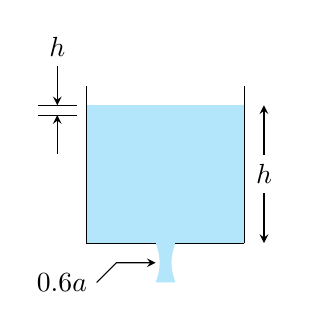
\begin{tikzpicture}
  [ragged border/.style={ decoration={random steps, segment length=1mm, amplitude=0.5mm},
           decorate,}]
\pgfmathsetmacro{\x}{2}
\pgfmathsetmacro{\y}{2}
\pgfmathsetmacro{\angA}{70}
\pgfmathsetmacro{\angB}{110}
%coloured water
\path(-\x/2-\x/16,0) to [out=-\angA,in=\angA]++(0,-\y/4)coordinate(kL);
\path(-\x/2+\x/16,0) to [out=-\angB,in=\angB]++(0,-\y/4)coordinate(kR);
\fill[cyan!30](-\x,\y-\y/8)--++(\x,0)-- ++(0,-\y+\y/8) --++ (-\x,0) --++ (0,\y-\y/8) -- cycle;
\fill[cyan!30] (-\x/2-\x/16,0) to [out=-\angA,in=\angA] (kL)--(kR) to [out=\angB,in=-\angB] ++(0,\y/4)--cycle;
\draw[stealth-stealth] (\x/8,0)--++(0,\y-\y/8)node[pos=0.5,fill=white]{$h$};
%drum
\draw(0,0)--++(0,\y);
\draw(0,0)--++(-\x/2+\x/16,0)++(-\x/8,0)--++(-\x/2+\x/16,0)--++(0,\y);
\draw[stealth-](-\x/2-\x/16,-\y/8)--++(-\x/4,0)--++(-\x/8,-\y/8)node[left]{$0.6a$};
\draw (-\x-\x/16,\y-\y/8)--++(-\x/4,0);
\draw (-\x-\x/16,\y-\y/8-\y/16)--++(-\x/4,0);
\draw[stealth-](-\x-\x/16-\x/8,\y-\y/8)--++(0,\y/4)node[above]{$\dif h$};
\draw[stealth-](-\x-\x/16-\x/8,\y-\y/8-\y/16)--++(0,-\y/4);
\end{tikzpicture}
\caption*{(الف)}
\end{subfigure}%
\begin{subfigure}{0.5\textwidth}
\centering
\begin{tikzpicture}
\pgfmathsetmacro{\x}{2}
\pgfmathsetmacro{\y}{2}
%water
\fill[cyan!10](0,0)--++(2*\x,0)--++(0,\y/8)--++(-2*\x,0)--cycle;
\fill[cyan!30](\x/2,0)--++(\x,0)--++(0,\y/8)--++(-\x,0)--cycle;
\draw[stealth-](-\x/8,\y/16)--++(-\x/4,0)node[pos=0.5,above]{$v$};
\draw[stealth-stealth](\x/2,-\y/8)--++(\x,0)node[pos=0.5,fill=white]{$v \Delta t$};
\draw(\x/2+\x/2,\y/16)--++(\x/2,\y/2)node[right]{$\Delta M=A v\Delta t$};
%pipe
\draw(0,\y/8)--++(2*\x,0);
\draw(0,0)--++(2*\x,0);
\draw[stealth-](\x/4,\y/8)--++(0,\y/4)--++(-\x/4,\y/4)node[above]{\RL{رقبہ عمودی تراش=$A$}};
\draw[dashed] (\x/2,-\y/4)node[below]{$m$}--++(0,\y/2);
\draw[dashed] (\x+\x/2,-\y/4)node[below]{$n$}--++(0,\y/2);

\end{tikzpicture}
\caption*{(ب)}
\end{subfigure}%
\caption{مثال \حوالہ{مثال_سادہ_اول_ٹاری_سلی}: پانی کا انخلا اور پانی کے دھار کا سکڑنا۔}
\label{شکل_مثال_سادہ_اول_ٹاری_سلی}
\end{figure}

حل:دورانیہ \عددی{\dif t} میں پانی کی انخلا کے بنا ٹینکی میں پانی کی گہرائی \عددی{\dif h} کم ہو گی جو \عددی{B \dif h} حجم کی کمی کو ظاہر کرتی ہے جہاں \عددی{B} ٹینکی کا رقبہ عمودی تراش ہے۔چونکہ پانی کے انخلا سے ٹینکی میں پانی کم ہوتا ہے لہٰذا درج ذیل لکھا جا سکتا ہے جو دیے گئے مسئلے کا تفرقی مساوات ہے۔
\begin{align}
0.6a\sqrt{2gh} \dif t=-B\dif h
\end{align}
متغیرات کو علیحدہ کرتے ہوئے حل کرتے ہیں۔
\begin{align*}
\frac{\dif h}{\sqrt{h}}=-\frac{0.6a \sqrt{2g}}{B} \dif t,\quad 2\sqrt{h}=-\frac{0.6a \sqrt{2g}}{B} t+c
\end{align*}
ابتدائی لمحہ \عددی{t=0} پر پانی کی گہرائی \عددی{h_1} ہے۔ان معلومات کو درج بالا میں پر کرتے ہوئے \عددی{c=2h_1} ملتا ہے لہٰذا تفرقی مساوات کا جبری حل درج ذیل ہے۔
\begin{align}\label{مساوات_سادہ_اول_ٹاری_سلی_ٹینکی_خالی}
 2\sqrt{h}=-\frac{0.6a \sqrt{2g}}{B} t+ 2\sqrt{h_1}
\end{align}
خالی ٹینکی سے مراد \عددی{h=0} ہے۔جبری حل میں \عددی{h=0} پر کرتے ہوئے ٹینکی خالی کرنے کے لئے درکار وقت حاصل کرتے ہیں۔
\begin{align*}
 2\sqrt{0}=-\frac{0.6a \sqrt{2g}}{B} t+ 2\sqrt{h_1}, \quad t=\frac{2\sqrt{h_1} B}{0.6a \sqrt{2g}}\\
t=\frac{2\sqrt{1.5} \times 2}{0.6\pi 0.005^2 \sqrt{2\times 9.8}}=\SI{23482}{\second} \approx \SI{6.52}{\hour}
\end{align*}
مساوات \حوالہ{مساوات_سادہ_اول_ٹاری_سلی_ٹینکی_خالی} کو شکل \حوالہ{شکل_مثال_سادہ_اول_ٹاری_سلی_خالی} میں دکھایا گیا ہے۔یاد رہے کہ \عددی{\SI{23482}{\second}} میں ٹینکی خالی ہو جاتی ہے لہٰذا ترسیم کو اتنے وقت کے لئے ہی کھینچا گیا ہے۔
\begin{figure}
\centering
\begin{tikzpicture}
\begin{axis}[axis lines*=middle,ylabel={$h$},ylabel style={rotate=-90},ylabel style={at={(axis description cs:0,1.05)}},xlabel={$t\, (\si{\second})$},scaled x ticks=false]
\pgfmathsetmacro{\ha}{1.5}
\pgfmathsetmacro{\B}{2}
\pgfmathsetmacro{\a}{pi*0.005^2}
%\pgfmathsetmacro{\k}{0.3*\a*sqrt(2*9.8)/\B}  %pgfmath calculate this value wrongly????
\pgfmathsetmacro{\k}{0.000052}
%
\addplot[domain=0:23480]({x},{(sqrt(\ha)-\k*x)^(2)});
\end{axis}
\end{tikzpicture}
\caption{مثال \حوالہ{مثال_سادہ_اول_ٹاری_سلی}: ٹینکی خالی ہونے کا عمل۔}
\label{شکل_مثال_سادہ_اول_ٹاری_سلی_خالی}
\end{figure}
\انتہا{مثال}
%======================

\جزوحصہء{علیحدگی متغیرات کی جامع ترکیب}
بعض اوقات نا قابل علیحدگی تفرقی مساوات کے متغیرات کو تبدیل کرتے ہوئے مساوات کو قابل علیحدگی بنایا جا سکتا ہے۔ اس ترکیب کو درج ذیل عملاً اہم قسم کی مساوات کے لئے سیکھتے ہیں جہاں \عددی{f(\tfrac{y}{x})} قابل تفرق تفاعل ہے مثلاً \عددی{\cos \tfrac{y}{x}}، \عددی{e^{(y/x)}} وغیرہ۔
\begin{align}
y'=f\left(\frac{y}{x}\right)
\end{align}  
مساوات کی صورت دیکھتے ہوئے \عددیء{\tfrac{y}{x}=u} لیتے ہیں۔یوں درج ذیل لکھا جا سکتا ہے
\begin{align}\label{مساوات_سادہ_اول_جامع_علیحدگی_الف}
y=ux,\quad y'=u+xu'
\end{align}
جنہیں \عددی{y'=f(\tfrac{y}{x})} میں پر کرتے ہوئے \عددی{u+xu'=f(u)} یعنی \عددی{xu'=f(u)-u} ملتا ہے۔اگر \عددی{f(u)-u \ne 0} ہو تب متغیرات علیحدہ کرتے ہوئے درج ذیل لکھا جا سکتا ہے۔
\begin{align} 
\frac{\dif u}{f(u)-u}=\frac{\dif x}{x}
\end{align}
%============
\ابتدا{مثال}
تفاعل \عددی{xy'-y=2x} کو حل کریں۔

حل:تفاعل کو \عددی{y'=\tfrac{y}{x}+2} لکھا جا سکتا ہے۔یوں \عددی{\tfrac{y}{x}=u} لیتے ہوئے  مساوات \حوالہ{مساوات_سادہ_اول_جامع_علیحدگی_الف} کے استعمال سے درج ذیل ملتا ہے۔
\begin{align*}
u+xu'=u+2, \quad \dif u=2\frac{\dif x}{x},\quad u=2\ln \abs{x}+c
\end{align*}
اس میں \عددی{u} کی جگہ واپس \عددی{\tfrac{y}{x}} پر کرتے ہوئے جواب حاصل ہوتا ہے۔
\begin{align*}
\frac{y}{x}=2\ln \abs{x}+c,\quad y=2x\ln \abs{x}+cx
\end{align*}
\انتہا{مثال}
%=========================

\حصہء{سوالات}
سوال \حوالہ{سوال_سادہ_اول_جامع_علیحدگی_الف} تا سوال \حوالہ{سوال_سادہ_اول_جامع_علیحدگی_ب} کے عمومی حل حاصل کریں۔حاصل حل کو واپس تفرقی مساوات میں پر کرتے ہوئے اس کی درستگی ثابت کریں۔

%=======================
\ابتدا{سوال}\شناخت{سوال_سادہ_اول_جامع_علیحدگی_الف}
$y^2y'+x^2=0$

جواب:\عددی{x^3+y^3=c}
\انتہا{سوال}
%=============================
\ابتدا{سوال}
$yy'+x=0$

جواب:\عددی{x^2+y^2=c}
\انتہا{سوال}
%=============================
\ابتدا{سوال}
$y'=\sec^2 y$

جواب:\عددی{y=\tan x+c}
\انتہا{سوال}
%=============================
\ابتدا{سوال}
$y'\cos x=y\sin x$

جواب:\عددی{y=c\sec x}
\انتہا{سوال}
%=============================
\ابتدا{سوال}
$y'=ye^{x-1}$

جواب:\عددی{\ln\abs{y}=e^{x-1}+c}
\انتہا{سوال}
%=============================
\ابتدا{سوال} 
\عددی{u=\tfrac{y}{x}} پر کرتے ہوئے \عددی{xy'=y+x^2\sin^2\frac{y}{x}} کو حل کریں۔

جواب:\عددی{\tfrac{\cos \tfrac{y}{x}-1}{\cos\tfrac{y}{x}+1}=ce^{2x}}
\انتہا{سوال}
%=============================
\ابتدا{سوال}
\عددی{y'=(2x+y)^2} کو حل کریں۔ایسا کرنے کی خاطر \عددی{u=2x+y} پر کرنا ہو گا۔

جواب:\عددی{y=-2x+\sqrt{2}\tan(\sqrt{2}x+c)}
\انتہا{سوال}
%=============================
\ابتدا{سوال} 
\عددی{u=\tfrac{y}{x}} پر کرتے ہوئے \عددی{xy'=y^2+y} کو حل کریں۔

جواب:\عددی{y=-\tfrac{x}{x+c}}
\انتہا{سوال}
%=============================
\ابتدا{سوال} \شناخت{سوال_سادہ_اول_جامع_علیحدگی_ب}
\عددی{u=\tfrac{y}{x}} پر کرتے ہوئے \عددی{xy'=x-y} کو حل کریں۔

جواب:\عددی{xy-x^2=c}
\انتہا{سوال}
%=============================

 ابتدائی قیمت سوال \حوالہ{سوال_سادہ_اول_ابتدائی_قیمت_الف} تا سوال \حوالہ{سوال_سادہ_اول_ابتدائی_قیمت_ب} کے جبری حل حاصل کریں۔

\ابتدا{سوال}\شناخت{سوال_سادہ_اول_ابتدائی_قیمت_الف}
\begin{align*}
xy'+y=0,\quad y(2)=8
\end{align*}

جواب:\عددی{y=\tfrac{16}{x}}
\انتہا{سوال}
%====================
\ابتدا{سوال}
\begin{align*}
y'=1+9y^2,\quad y(1)=0
\end{align*}

جواب:\عددی{y=\tfrac{1}{3}\tan[3(x-1)]}
\انتہا{سوال}
%======================
\ابتدا{سوال}
\begin{align*}
y' \cos^2 x=\sin^2 y, \quad y(0)=\frac{\pi}{4}
\end{align*}

جواب:\عددی{\tan y=\tfrac{1}{1-\tan x}}
\انتہا{سوال}
%==============================
\ابتدا{سوال}
\begin{align*}
y'=-4xy,\quad y(0)=5
\end{align*}

جواب:\عددیء{y=5e^{-2x^2}}
\انتہا{سوال}
%==================
\ابتدا{سوال}
\begin{align*}
y'=-\frac{2x}{y},\quad y(1)=2
\end{align*}

جواب:\عددی{2x^2+y^2=6}
\انتہا{سوال}
%==================
\ابتدا{سوال}
\begin{align*}
y'=(x+y-4)^2,\quad y(0)=5
\end{align*}

جواب:\عددی{x+y-4=\tan(x+\tfrac{\pi}{4})}
\انتہا{سوال}
%=================
\ابتدا{سوال}\شناخت{سوال_سادہ_اول_ابتدائی_قیمت_ب}
\begin{align*}
xy'=y+3x^4\cos^2 \frac{y}{x},\quad y(1)=0
\end{align*}

 جواب:اس میں \عددی{u=\tfrac{y}{x}} پر کرنے سے \عددی{\tan \tfrac{y}{x}=x^3-1} ملتا ہے۔
\انتہا{سوال}
%=================
\ابتدا{سوال}
کسی بھی لمحے پر جرثوموں کی تعداد بڑھنے کی شرح، اس لمحے موجود جرثوموں کی تعداد کے راست تناسب ہے۔اگر ان کی تعداد دو گھنٹوں میں دگنی ہو جائے تب چار گھنٹوں بعد ان کی تعداد کتنی ہو گی؟ چوبیس گھنٹوں بعد کتنی ہو گی؟  

جوابات:\عددی{y=y_0e^{0.34657t}}، \عددی{4y_0}، \عددی{4095y_0}
\انتہا{سوال}
%==================
\ابتدا{سوال}
جرثوموں کی شرح پیدائش موجودہ تعداد کے راست تناسب ہے۔ان کی شرح اموات بھی موجودہ تعداد کے راست تناسب ہے۔جرثوموں کی تعداد بڑھنے کی شرح کیا ہو گی؟ تعداد بالمقابل وقت کیا ہو گا؟ تعداد کہاں متوازن صورت اختیار کرے گی؟

جوابات:\عددی{\tfrac{\dif y}{\dif t}=\alpha y-\beta y} جہاں \عددی{\alpha} اور \عددی{\beta} بالترتیب پیدائشی اور امواتی راست تناسب کے مستقل ہیں۔ تعداد بالمقابل وقت کی مساوات \عددیء{y=y_0e^{(\alpha-\beta)t}} ہے۔اگر \عددی{\alpha > \beta} ہو تب تعداد بڑھتی رہے گی۔اس کے برعکس اگر \عددی{\alpha<\beta} ہو تب تعداد گھٹتی رہے گی حتٰی کہ جراثیم فنا ہو جائیں اور \عددی{\alpha=\beta} کی صورت میں تعداد وقت کے ساتھ تبدیل نہیں ہو گی۔ 
\انتہا{سوال}
%=================
\ابتدا{سوال}
عموماً جاندار مرنے کے بعد مکمل طور پر خاک میں مل جاتے ہیں اور ان کا نشان تک نہیں رہتا البتہ بعض اوقات حالات یوں ہوتے ہیں کہ ان کا جسم پتھر میں بدل جاتا ہے۔اس پتھریلی جسم میں موجود \عددی{\ce{^{14}_{6}C}} اور \عددی{\ce{^{12}_{6}C}} ہم جا کے تناسب  سے اس کی عمر کا تخمینہ لگایا جا سکتا ہے۔ دو ہزار سال پرانی پتھریلی مچھلی  میں کاربن کا تناسب، ابتدائی تناسب کے کتنا گنا ہو گا؟

جواب:\عددی{\SI{69.5}{\percent}}
\انتہا{سوال}
%================
\ابتدا{سوال}
طبیعیات میں \اصطلاح{بار بردار}\فرہنگ{بار بردار}\حاشیہب{charged}\فرہنگ{charged} ذروں کو \اصطلاح{مسرع خطی}\فرہنگ{مسرع خطی}\حاشیہب{linear accelerator}\فرہنگ{linear accelerator} کے ذریعہ اسراع دی جاتی ہے۔تصور کریں کہ مسرع خطی میں \عددی{\ce{^{4}_{2}He^{2+}}} داخل ہوتا ہے جس کی رفتار مستقل اسراع کے ساتھ \عددی{\SI{1.2}{\milli\second}} دورانیے میں \عددی{\SI{e3}{\meter\per\second}} سے بڑھا کر \عددی{\SI{1.6e4}{\meter\per\second}} کر دی جاتی ہے۔اسراع دریافت کریں۔اس دورانیے میں ذرہ کتنا فاصلہ طے کرتا ہے؟

جوابات:\عددی{\SI{1.25e7}{\meter\per\second\squared}}، \عددی{\SI{10.2}{\meter}} 
\انتہا{سوال}
%==================
\ابتدا{سوال}
ایک ٹینکی میں \عددیء{2000} لٹر پانی پایا جاتا ہے جس میں \عددی{\SI{150}{\kilo\gram}} نمک ملایا گیا ہے۔پانی کو مسلسل ہلانے سے کثافت یکساں رکھی جاتی ہے۔ٹینکی میں \عددی{10} لٹر فی منٹ تازہ پانی شامل کیا جاتا ہے۔ٹینکی سے پانی کا اخراج بھی \عددی{10} لٹر فی منٹ ہے۔ایک گھنٹہ بعد ٹینکی میں کل کتنا نمک پایا جائے گا؟

جوابات:\عددی{y=150e^{-\tfrac{t}{200}}}، \عددی{y=\SI{111}{\kilo\gram}}
\انتہا{سوال}
%===================
\ابتدا{سوال}
مریض کے زبان کے نیچے تھرمامیٹر رکھ کر اس کا درجہ حرارت ناپا جاتا ہے۔ کمرے اور مریض کے درجہ حرارت بالترتیب \عددی{\SI{25}{\degree\celsius}} اور \عددی{\SI{40}{\degree\celsius}} ہیں۔زبان کے نیچے رکھنے کے ایک منٹ بعد تھرمامیٹر کا پارہ \عددی{\SI{35}{\degree\celsius}} تک پہنچتا ہے۔ تھرمامیٹر کتنی دیر میں اصل درجہ حرارت کے قریب (مثلاً \عددی{\SI{39.9}{\degree\celsius}}) پہنچ پائے گا؟

جواب:\عددی{T=40-15e^{-1.204t}}، \عددی{t=\SI{4.16}{\minute}}
\انتہا{سوال}
%====================
\ابتدا{سوال}
\اصطلاح{سرطان}\فرہنگ{سرطان}\حاشیہب{cancer}\فرہنگ{cancer} کی مہلک بیماری میرے خاندان کے کئی افراد کی جان لے چکی ہے۔سن \عددی{1960} میں اینا کین لایرڈ\حاشیہب{Anna Kane Laird} سرطان کی رسولی کی افزائش کو ٹھیک طرح \اصطلاح{گامپرٹز تفاعل}\فرہنگ{گامپرٹز تفاعل}\فرہنگ{تفاعل!گامپرٹز}\فرہنگ{سرطان!گامپرٹز}\حاشیہب{Benjamin Gompertz}\فرہنگ{Benjamin Gompertz} سے ظاہر کرنے میں کامیاب ہوئے۔

سرطانی رسولی میں جسم کا نظام تباہ ہو جاتا ہے۔یوں رسولی میں موجود خلیوں تک آکسیجن اور خوراک کا پہنچنا ممکن نہیں رہتا۔رسولی کے اندرونی خلیے آکسیجن اور خوراک کی کمی کی بنا مر جاتے ہیں۔ان حقائق کی نمونہ کشی درج ذیل گامپرٹز تفرقی مساوات کرتی ہے جہاں \عددی{y} رسولی کی کمیت ہے۔
\begin{align}
y'=-Ay\ln y,\quad A>0
\end{align}

جواب:\عددی{\ln y=ce^{-At}}
\انتہا{سوال}
%===================
\ابتدا{سوال}
دھوپ میں کپڑے کی نمی خشک ہونی کی شرح کپڑے میں موجود نمی کے راست تناسب ہوتی ہے۔اگر پہلے پندرہ منٹ میں نصف پانی خشک ہو جائے تب  \عددی{\SI{99.9}{\percent}} پانی کتنی دیر میں خشک ہو گا؟ ہم  \عددی{\SI{99.9}{\percent}} خشک کو مکمل خشک تصور کر سکتے ہیں۔

جواب:\عددی{y=y_0e^{-0.0462t}}، \عددی{\SI{49.8}{\minute}}
\انتہا{سوال}
%==================
\ابتدا{سوال}\شناخت{سوال_سادہ_اول_رگڑ}\quad رگڑ \\
دو سطحوں کو آپس میں رگڑنے سے قوت رگڑ پیدا ہوتی ہے جو اس حرکت کو روکنے کی کوشش کرتی ہے۔خشک سطحوں پر پیدا قوت \عددی{\abs{F}=\mu \abs{N}} سے حاصل کی جا سکتی ہے جہاں \عددی{N} دونوں سطحوں پر عمودی قوت، \عددی{\mu} \اصطلاح{حرکی رگڑ کا مستقل}\فرہنگ{حرکی رگڑ کا مستقل}\فرہنگ{رگڑ!حرکی مستقل}\حاشیہب{coefficient of kinetic friction}\فرہنگ{friction!coefficient} اور \عددی{F} رگڑ سے پیدا قوت ہے۔
\begin{figure}
\centering
\begin{subfigure}{0.5\textwidth}
\centering
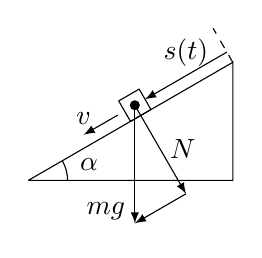
\begin{tikzpicture}
\pgfmathsetmacro{\len}{3}
\pgfmathsetmacro{\ang}{30}
\pgfmathsetmacro{\x}{\len*cos(\ang)}
\pgfmathsetmacro{\y}{\len*sin(\ang)}
\pgfmathsetmacro{\lenF}{1.5}
\pgfmathsetmacro{\xF}{\lenF*cos(\ang)}
\pgfmathsetmacro{\yF}{\lenF*sin(\ang)}
%
\draw (0,0)--++(\x,0)--++(0,\y)--(0,0);
\draw(\ang:1/2*\len)coordinate(kL) --++ (\ang:0.3)coordinate(A)--++(\ang+90:0.3)coordinate(B)--++(180+\ang:0.3)--++(\ang-90:0.3);
\draw([shift={(0:0.5)}]0,0) arc (0:\ang:0.5);
\draw(\ang/2:0.8)node{$\alpha$};
\draw[-latex] (kL)++(\ang+90:0.15)++(\ang:-0.1)--++(\ang:-0.5)node[above]{$v$};
\draw[dashed](\ang:\len)coordinate(C)--++(\ang+90:0.5)coordinate(D);
\draw[latex-]($(A)!0.5!(B)$)coordinate(E)--($(C)!(E)!(D)$)node[pos=0.5,above]{$s(t)$};
\draw[-latex](\ang:1/2*\len+0.15)++(\ang+90:0.15)node[circ]{}--++(0,-\lenF)node[pos=0.9,left]{$mg$}coordinate(Ftip);
\draw[latex-](Ftip)--++(\ang:\yF)coordinate(Htip);
\draw[latex-](Htip)--++(\ang+90:\xF)node[pos=0.5,right]{$N$};
\end{tikzpicture}
\caption*{(الف)}
\end{subfigure}%
\begin{subfigure}{0.5\textwidth}
\centering
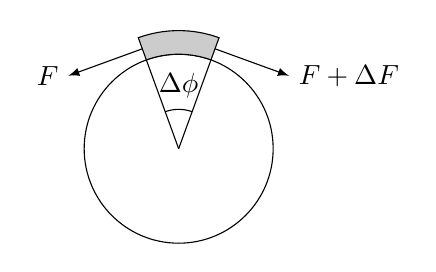
\begin{tikzpicture}
\pgfmathsetmacro{\angA}{70}
\pgfmathsetmacro{\angB}{110}
\draw(0,0) circle (1.2cm);
\draw[fill=gray!40] ([shift={(\angA:1.2cm)}]0,0) arc (\angA:\angB:1.2cm) --++(\angB:0.3cm) arc (\angB:\angA:1.5cm) --++(\angA:-0.3cm);
\draw(0,0)--++(\angA:1.2cm);
\draw(0,0)--++(\angB:1.2cm);
\draw([shift={(\angA:0.5)}]0,0)  arc (\angA:\angB:0.5);
\draw(\angA/2+\angB/2:0.8)node{$\Delta \phi$};
\draw[-latex] (\angA:1.35cm)--++(\angA-90:1cm)node[right]{$F+\Delta F$};
\draw[-latex] (\angB:1.35cm)--++(\angB+90:1cm)node[left]{$F$};
\end{tikzpicture}
\caption*{(ب)}
\end{subfigure}%
\caption{سوال \حوالہ{سوال_سادہ_اول_رگڑ} اور سوال \حوالہ{سوال_سادہ_اول_رسی_رگڑ} کے اشکال۔}
\label{شکل_سوال_سادہ_اول_رگڑ}
\end{figure}

شکل \حوالہ{شکل_سوال_سادہ_اول_رگڑ}-الف میں \عددی{\alpha} زاویہ کی سطح پر \عددی{m} کمیت کا جسم دکھایا گیا ہے۔اس پر ثقلی قوت (وزن) \عددی{mg} عمل کرتا ہے۔اس قوت کو دو حصوں میں تقسیم کیا جا سکتا ہے۔پہلا حصہ \عددی{N} ہے جو سطح کے عمودی ہے۔دوسرا حصہ سطح کے متوازی ہے جو جسم کو اسراع دیتا ہے۔  کمیت \عددی{\SI{10}{\kilo\gram}}، ثقلی اسراع \عددی{g=\SI{9.8}{\meter\per\second\squared}}، رگڑ کا مستقل \عددی{\mu=0.25} اور زاویہ \عددی{\alpha=\SI{30}{\degree}} ہیں۔ ابتدائی رفتار صفر لیتے ہوئے رفتار \عددی{v} کی مساوات حاصل کریں۔یہ جسم کتنی دیر میں کل \عددی{\SI{15}{\meter}} فاصلہ طے کرے گا؟

جواب: \عددی{mg\sin \alpha-\mu mg\cos \alpha=m\tfrac{\dif v}{\dif t}}، \عددی{v=3.93t\,\si{\meter\per\second}}، \عددی{\SI{2.76}{\second}}
\انتہا{سوال}
%===================
\ابتدا{سوال}\شناخت{سوال_سادہ_اول_رسی_رگڑ}
شکل \حوالہ{شکل_سوال_سادہ_اول_رگڑ}-ب میں گول جسم کے گرد لپیٹی گئی رسی کا چھوٹا حصہ دکھایا گیا ہے۔تجربے سے معلوم ہوتا ہے کہ رسی کے چھوٹے حصے کے سروں پر قوت میں فرق زاویہ \عددی{\Delta \phi} اور قوت \عددی{F} کے راست متناسب ہوتا ہے۔رسی کو جسم کے گرد کتنی مرتبہ لپیٹنے سے ایک شخص \عددی{500} گنا زیادہ قوت کے گاڑی کو روک سکتا ہے؟

جوابات:\عددی{F=F_0e^{\phi}}، \عددی{\phi=\SI{6.21}{\radian}} یعنی \عددی{1.98} مرتبہ لپیٹنا ضروری ہے۔
\انتہا{سوال}
%====================
\ابتدا{سوال}
کارتیسی محدد کے محور پر گول دائرے \عددی{x^2+y^2=r^2} کا تفرقی مساوات \عددی{y_1'} حاصل کریں۔اسی طرح محور سے گزرتے ہوئے سیدھے خط کا تفرقی مساوات \عددی{y_2'} حاصل کریں۔دونوں تفرقی مساوات کا حاصل ضرب کیا ہو گا؟ اس حاصل ضرب سے آپ کیا اخذ کر سکتے ہیں؟

جواب:\عددی{y_1' y_2'=-1}؛ آپس میں عمودی ہیں۔
\انتہا{سوال}
%=====================
\ابتدا{سوال}
آپ کو ایسے تفاعل سے ضرور واسطہ پڑیگا جس کا تحلیلی تکمل حاصل کرنا ممکن نہیں ہو گا۔ایسا ایک تفاعل \عددی{e^{x^2}} ہے۔اس تفاعل کی \اصطلاح{مکلارن تسلسل}\فرہنگ{تسلسل!مکلارن}\فرہنگ{مکلارن تسلسل}\حاشیہب{Maclaurin's series}\فرہنگ{Maclaurin's series} کے پہلے چار ارکان کا تکمل حاصل کریں۔

جواب:\عددی{\int e^{x^2} \approx x+\tfrac{x^3}{3}+\tfrac{x^5}{10}+\tfrac{x^7}{36}+\cdots}
\انتہا{سوال}
%========================
\ابتدا{سوال}\شناخت{سوال_سادہ_اول_کرہ_ٹینکی}\quad قانون ٹاری سلی\\
کروی ٹینکی کا رداس \عددی{R} ہے۔اس کی تہہ میں چھوٹا سوراخ ہے جس کا رداس \عددی{r} ہے۔پوری طرح بھری ہوئی ٹینکی کتنی دیر میں خالی ہو گی۔اگر \عددی{R=\SI{1}{\meter}} اور \عددی{r=\SI{1}{\centi\meter}} ہو تب ٹینکی کتنی دیر میں خالی ہو گی؟

جواب:\عددی{0.6\pi r^2 \sqrt{2 g h } \dif t=-\pi[R^2+(h-R)^2]\dif h}،\\
 \عددی{t+c=-\tfrac{\sqrt{2gh}}{9gr^2}(30R^2-10hR+3h^2)}،\quad  \عددی{t_{\text{خالی}}=\tfrac{44R^2\sqrt{gR}}{9gr^2}}،\\
 دیے رداس کی ٹینکی \عددی{\SI{4.34}{\hour}} یعنی چار گھنٹے اور بیس منٹ میں خالی ہو گی۔
\انتہا{سوال}
%======================

\حصہ{قطعی سادہ تفرقی مساوات اور جزو تکمل}\شناخت{حصہ_سادہ_اول_جزو_تکمل}
ایسا تفاعل \عددی{u(x,y)} جس کے \اصطلاح{بلا جوڑ}\فرہنگ{بلا جوڑ}\حاشیہب{continuous partial differential}\فرہنگ{continuous!partial differential} جزوی تفرق پائے جاتے ہوں کا (مکمل) تفرق درج ذیل ہے۔
\begin{align}
\dif u=\frac{\partial u}{\partial x}\dif x+\frac{\partial u}{\partial y}\dif y
\end{align}
یوں اگر \عددی{u(x,y)=c} ہو تب \عددی{\dif u=0} ہو گا۔

مثال کے طور پر \عددی{u=xy+2(x-y)=7} کا تفرق
\begin{align*}
\dif u=(y+2)\dif x+(x-2)\dif y=0
\end{align*}
ہو گا جس سے درج ذیل تفرقی مساوات لکھی جا سکتی ہے۔
\begin{align*}
y'=\frac{\dif y}{\dif x}=-\frac{y+2}{x-2}
\end{align*}
الٹ چلتے ہوئے اس تفرقی مساوات کو ہم حل کر سکتے ہیں۔ اس مثال سے ایک ترکیب جنم دیتی ہے جس پر اب غور کرتے ہیں۔

درجہ اول سادہ تفرقی مساوات \عددی{y'=-\tfrac{M(x,y)}{N(x,y)}} یعنی
\begin{align}\label{مساوات_سادہ_اول_قطعی_الف}
M(x,y)\dif x+N(x,y)\dif y=0
\end{align}
کو اس صورت \اصطلاح{قطعی تفرقی مساوات}\فرہنگ{قطعی تفرقی مساوات}\فرہنگ{تفرقی مساوات!قطعی}\حاشیہب{exact differential equation}\فرہنگ{exact differential equation} کہتے ہیں جب اس کو درج ذیل لکھنا ممکن ہو جہاں \عددی{u(x,y)} کوئی تفاعل ہے۔
\begin{align}\label{مساوات_سادہ_اول_قطعی_ب}
\frac{\partial u}{\partial x}\dif x+\frac{\partial u}{\partial y}\dif y=0
\end{align}
یوں مساوات \حوالہ{مساوات_سادہ_اول_قطعی_الف} کو
\begin{align}
\dif u=0
\end{align}
لکھ کر تکمل لیتے ہوئے تفرقی مساوات کا عمومی \اصطلاح{خفی حل}\فرہنگ{خفی حل}\حاشیہب{implicit solution}\فرہنگ{implicit solution}
\begin{align}
u(x,y)=c
\end{align}
حاصل ہوتا ہے۔

مساوات \حوالہ{مساوات_سادہ_اول_قطعی_الف} اور مساوات \حوالہ{مساوات_سادہ_اول_قطعی_ب} کا موازنہ کرتے ہوئے ہم دیکھتے ہیں کہ مساوات \حوالہ{مساوات_سادہ_اول_قطعی_الف} تب قطعی تفرقی مساوات ہو گا جب ایسا \عددی{u(x,y)} پایا جاتا ہو کہ درج ذیل لکھنا ممکن ہو۔
\begin{align}
\frac{\partial u}{\partial x}&=M \label{مساوات_سادہ_اول_قطعی_شرط_الف}\\
\frac{\partial u}{\partial y}&=N\label{مساوات_سادہ_اول_قطعی_شرط_ب}
\end{align}
ان سے ہم تفرقی مساوات کے قطعی ہونے کا شرط اخذ کرتے ہیں۔

سطح \عددی{xy} پر ایسا خطہ جس کا سرحد بند منحنی ہو اور یہ منحنی اپنے آپ کو نہ کاٹتا ہو پر تصور کریں کہ  \عددی{M} اور \عددی{N} ایسے \اصطلاح{بے جوڑ}\فرہنگ{بے جوڑ تفاعل}\حاشیہب{continuous}\فرہنگ{continuous function} (یعنی \اصطلاح{استمراری}) تفاعل ہیں جن کے درجہ اول تفرق بھی اس خطے پر بے جوڑ ہیں۔تب مساوات \حوالہ{مساوات_سادہ_اول_قطعی_شرط_الف} کے تفرق درج ذیل ہوں گے۔
\begin{align*}
\frac{\partial M}{\partial y}&=\frac{\partial^2 u}{\partial y \partial x}\\
\frac{\partial N}{\partial x}&=\frac{\partial^2 u}{\partial x \partial y}
\end{align*}
استمراری شرط کی بنا  \عددی{\tfrac{\partial^2 u}{\partial y \partial x}} اور \عددی{\tfrac{\partial^2 u}{\partial x \partial y}} برابر ہیں لہٰذا درج ذیل لکھا جا سکتا ہے۔
\begin{align}\label{مساوات_سادہ_اول_قطعی_تفرقی_شرط}
\frac{\partial M}{\partial y}=\frac{\partial N}{\partial x}
\end{align}
مساوات \حوالہ{مساوات_سادہ_اول_قطعی_الف} کا قطعی تفرقی مساوات ہونے کے لئے مساوات \حوالہ{مساوات_سادہ_اول_قطعی_تفرقی_شرط} پر پورا اترنا \اصطلاح{لازمی}\فرہنگ{شرط!لازمی}\فرہنگ{لازمی شرط!قطعی تفرقی}\حاشیہب{necessary condition}\فرہنگ{necessary condition!exactness} اور  \اصطلاح{کافی}\فرہنگ{کافی!قطعی تفرقی}\حاشیہب{sufficient condition}\فرہنگ{sufficient condition!exactness} ہے۔

قطعی تفرقی مساوات کا حل حاصل کرتے ہیں۔مساوات \حوالہ{مساوات_سادہ_اول_قطعی_شرط_الف} کا \عددی{x} تکمل لیتے ہوئے درج ذیل لکھا جا سکتا ہے
\begin{align}\label{مساوات_سادہ_اول_قطعی_حل_الف}
u=\int M \dif x+k(y)
\end{align}
جہاں تکمل کا مستقل  از خود \عددی{y} کا تفاعل ہو سکتا ہے۔تکمل کا مستقل \عددی{k(y)} حاصل کرنے کی خاطر مساوات \حوالہ{مساوات_سادہ_اول_قطعی_حل_الف} کا جزوی تفرق  \عددی{\tfrac{\partial u}{\partial y}} لیتے ہوئے  مساوات \حوالہ{مساوات_سادہ_اول_قطعی_شرط_ب} کی مدد سے  \عددی{\tfrac{\dif k}{\dif y}} حاصل کرتے ہیں جس کا \عددی{y} تکمل لینے سے \عددی{k} حاصل ہو گا۔(مثال \حوالہ{مثال_سادہ_اول_قطعی_مساوات_الف} دیکھیں۔)

اسی طرح مساوات \حوالہ{مساوات_سادہ_اول_قطعی_شرط_ب}  کا \عددی{y} تکمل لیتے ہوئے درج ذیل لکھا جا سکتا ہے
\begin{align}\label{مساوات_سادہ_اول_قطعی_حل_ب}
u=\int N \dif y + m(x)
\end{align}
جہاں تکمل کا مستقل از خود \عددی{x} کا تفاعل ہو سکتا ہے۔تکمل کا مستقل \عددی{m(x)} حاصل کرنے کی خاطر مساوات \حوالہ{مساوات_سادہ_اول_قطعی_حل_ب} کا جزوی تفرق  \عددی{\tfrac{\partial u}{\partial x}} لیتے ہوئے  مساوات \حوالہ{مساوات_سادہ_اول_قطعی_شرط_الف} کی مدد سے \عددی{\tfrac{\dif m}{\dif x}=} حاصل کرتے ہیں جس کا \عددی{x} تکمل لینے سے \عددی{m} حاصل ہو گا۔

%==================
\ابتدا{مثال}\شناخت{مثال_سادہ_اول_قطعی_مساوات_الف}\quad قطعی تفرقی مساوات\\
درج ذیل کو حل کریں۔
\begin{align}\label{مساوات_سادہ_اول_مثال_قطعی_الف}
(1+2xy^3)\dif x+(2y+3x^2y^2)\dif y=0
\end{align}

حل:پہلے ثابت کرتے ہیں کہ یہ مساوات \اصطلاح{قطعی} ہے۔یہ مساوات \حوالہ{مساوات_سادہ_اول_قطعی_الف} کی طرح ہے جہاں
\begin{align*}
M&=1+2xy^3\\
N&=2y+3x^2y^2
\end{align*}
ہیں۔ \عددی{\tfrac{\partial M}{\partial y}} اور \عددی{\tfrac{\partial N}{\partial y}} لکھتے ہیں
\begin{align*}
\frac{\partial M}{\partial y}&=6xy^2\\
\frac{\partial N}{\partial x}&=6xy^2
\end{align*}
جو مساوات \حوالہ{مساوات_سادہ_اول_قطعی_تفرقی_شرط} پر پورا اترتے ہیں لہٰذا دی گئی مساوات قطعی تفرقی مساوات  ہے۔آئیں اب اس کو حل کرتے ہیں۔

مساوات \حوالہ{مساوات_سادہ_اول_قطعی_حل_الف} کو استعمال کرتے ہیں۔
\begin{align}\label{مساوات_سادہ_اول_قطعی_حل_پ}
u=\int (1+2xy^3)\dif x+k(y)=x+x^2y^3+k(y) 
\end{align}
اس کا \عددی{y} جزوی تفرق لیتے ہوئے مساوات \حوالہ{مساوات_سادہ_اول_قطعی_شرط_ب} کا استعمال کرتے
\begin{align*}
\frac{\partial u}{\partial y}=3x^2y^2+\frac{\dif k}{\dif y}=N=2y+3x^2y^2
\end{align*}
ہوئے \عددی{\tfrac{\dif k}{\dif y}} حاصل ہوتا ہے۔
\begin{align*}
\frac{\dif k}{\dif y}=2y
\end{align*}
اس کا \عددی{y} تکمل لیتے ہوئے \عددی{k} حاصل کرتے ہیں
\begin{align} \label{مساوات_سادہ_اول_قطعی_حل_ت}
k=\int 2y \dif y=y^2+c_1
\end{align}
جہاں \عددی{c_1} تکمل کا مستقل ہے۔چونکہ \عددی{k} صرف  \عددی{y} پر منحصر ہے لہٰذا \عددی{c_1} مستقل \عددی{x} پر منحصر نہیں ہو سکتا۔یوں مساوات \حوالہ{مساوات_سادہ_اول_قطعی_حل_پ} اور مساوات \حوالہ{مساوات_سادہ_اول_قطعی_حل_ت} سے قطعی تفرقی مساوات کا حاصل ہوتا ہے۔
\begin{align}\label{مساوات_سادہ_اول_قطعی_حل_ٹ}
u(x,y)=x+x^2y^3+y^2+c_1=0
\end{align}
آخر میں مساوات \حوالہ{مساوات_سادہ_اول_قطعی_حل_ٹ} کا تفرق لیتے ہوئے مساوات  \حوالہ{مساوات_سادہ_اول_مثال_قطعی_الف} حاصل کر کے حاصل حل کی درستگی ثابت کرتے ہیں۔
\begin{align*}
\dif u=\frac{\partial u}{\partial x}\dif x+\frac{\partial u}{\partial y}\dif y=(1+2xy^3)\dif x+(3x^2y^2+2y)\dif y
\end{align*}

\انتہا{مثال}
%===================
\ابتدا{مثال}\quad جبری حل\\
\عددی{N=2y+3x^2y^2} لیتے ہوئے مساوات \حوالہ{مساوات_سادہ_اول_مثال_قطعی_الف} کو حل کریں  جہاں \عددی{x=1} پر \عددی{y=2} ہے۔

حل:\عددی{\tfrac{\partial u}{\partial y}=N=2y+3x^2y^2} کا \عددی{y} تکمل
\begin{align}\label{مساوات_سادہ_اول_قطعی_دوسرا_متغیر}
u=\int (2y+3x^2y^2)\dif y+m(x)=y^2+x^2y^3+m(x)
\end{align} 
لے کر اس سے \عددی{\tfrac{\partial u}{\partial x}} لکھتے ہیں
\begin{align*}
\frac{\partial u}{\partial x}=2xy^3+\frac{\dif m}{\dif x}
\end{align*}
جو \عددی{M} کے برابر ہو گا
\begin{align*}
2xy^3+\frac{\dif m}{\dif x}=M=1+2xy^3
\end{align*}
جس سے
\begin{align*}
\frac{\dif m}{\dif x}=1, \quad m=x+c_2
\end{align*}
حاصل ہوتا ہے۔اس کو مساوات \حوالہ{مساوات_سادہ_اول_قطعی_دوسرا_متغیر} میں پر کرتے ہوئے تفرقی مساوات کا حل ملتا ہے۔
\begin{align*}
u=y^2+x^2y^3+x+c_2=0
\end{align*}
ابتدائی معلومات پر کرتے ہوئے
\begin{align*}
2^2+(1^2) (2^3)+1+c_2=0, \quad c=-13
\end{align*}
ملتا ہے جس سے جبری حل لکھتے ہیں۔
\begin{align*}
y^2+x^2y^3+x-13=0
\end{align*}
\انتہا{مثال}
%====================
\ابتدا{مثال}\شناخت{مثال_سادہ_اول_غیر_خطی}\quad غیر قطعی مساوات\\
مساوات \عددی{-y\dif x+x\dif y=0} میں \عددی{M=-y} اور \عددی{N=x} ہیں لہٰذا \عددی{\tfrac{\partial M}{\partial y}=-1} لیکن \عددی{\tfrac{\partial N}{\partial x}=1} ہے۔یوں دیا گیا مساوات \اصطلاح{غیر قطعی}\فرہنگ{غیر قطعی}\فرہنگ{قطعی!غیر}\حاشیہب{non exact}\فرہنگ{non exact} ہے۔یوں قطعی مساوات کی ترکیب قابل استعمال نہیں ہے۔آئیں قطعی مساوات کی ترکیب استعمال کرنے کی کوشش کریں۔مساوات \حوالہ{مساوات_سادہ_اول_قطعی_حل_الف} سے
\begin{align*}
u=\int -y \dif x+k(y)=-xy+k(y)
\end{align*}
ملتا ہے جس کا \عددیء{y} تفرق \عددی{\tfrac{\partial u}{\partial y}=-x+\tfrac{\dif k}{\dif y}} ہے جسے \عددی{N} یعنی \عددی{x} کے برابر پر کرنے سے 
\عددی{\tfrac{\dif k}{\dif y}=2x} ملتا ہے جس کا تکمل \عددی{k=2xy+c} ہے۔اب مستقل \عددی{k} صرف \عددی{y} پر منحصر ہو سکتا ہے جبکہ حاصل \عددی{k} اس شرط پر پورا نہیں اترتا لہٰذا اس کو رد کیا جاتا ہے۔یوں قطعی تفرقی مساوات کی ترکیب اس مثال میں دیے تفرقی مساوات کے حل کے لئے نا قابل استعمال ہے۔آپ \عددی{N} سے شروع کرتے ہوئے حل کرنے کی کوشش کر سکتے ہیں۔آپ اس راستے سے بھی حل حاصل نہیں کر پائیں گے۔
\انتہا{مثال}
%====================

\جزوحصہء{تخفیف بذریعہ جزو تکمل}
مثال \حوالہ{مثال_سادہ_اول_غیر_خطی} میں تفاعل \عددی{-y\dif x+x\dif y=0} غیر قطعی تھا البتہ اس کو \عددی{\tfrac{1}{x^2}} سے ضرب دینے
 سے \عددی{-\tfrac{y}{x^2}\dif x+\tfrac{1}{x}\dif y=0} حاصل ہوتا ہے جو قطعی مساوات  ہے۔آپ مساوات \حوالہ{مساوات_سادہ_اول_قطعی_تفرقی_شرط} استعمال کرتے ہوئے ثابت کر سکتے ہیں کہ یہ واقعی قطعی مساوات ہے۔حاصل قطعی مساوات کا حل حاصل کرتے ہیں۔
\begin{align}\label{مساوات_سادہ_اول_جزو_تکمل_الف}
-\tfrac{y}{x^2}\dif x+\tfrac{1}{x}\dif y=0, \quad \dif \left(\frac{y}{x}\right)=0,\quad \frac{y}{x}=c
\end{align}
اس ترکیب کو عمومی بناتے ہوئے ہم کہتے ہیں کہ غیر قطعی مساوات مثلاً
\begin{align}\label{مساوات_سادہ_اول_جزو_تکمل_حصول_الف}
P(x,y)\dif x+Q(x,y)\dif y=0
\end{align}
کو ایک مخصوص تفاعل \عددی{F} سے ضرب دینے سے قطعی مساوات
\begin{align}
FP\dif x+FQ\dif y=0
\end{align}
حاصل کی جا سکتی ہے۔تفاعل \عددی{F} \اصطلاح{جزو تکمل}\فرہنگ{جزو تکمل}\فرہنگ{تکمل!جزو}\حاشیہب{integrating factor}\فرہنگ{integrating factor} کہلاتا ہے اور یہ عموماً \عددی{x} اور \عددی{y} پر منحصر ہو گا۔حاصل قطعی مساوات کو حل کرنا ہم سیکھ چکے ہیں۔

%======================
\ابتدا{مثال}\quad جزو تکمل\\
مساوات \حوالہ{مساوات_سادہ_اول_جزو_تکمل_الف} میں جزو تکمل \عددی{\tfrac{1}{x^2}} تھا لہٰذا اس کا حل درج ذیل لکھا جا سکتا ہے۔
\begin{align*}
FP\dif x+FQ\dif y=\frac{-y\dif x+x\dif y}{x^2}=\dif \left(\frac{y}{x}\right)=0,\quad \frac{y}{x}=c
\end{align*}
مساوات \عددی{-y\dif x+x\dif y=0} کے  مزید جزو تکمل \عددی{\tfrac{1}{y^2}}، \عددی{\tfrac{1}{xy}} اور \عددی{\tfrac{1}{x^2+y^2}} ہیں جن سے درج ذیل لکھا جا سکتا ہے۔
\begin{align*}
\frac{-y\dif x+x\dif y}{y^2}&=\dif \left(\frac{x}{y}\right)=0, \quad \frac{x}{y}=c\\
\frac{-y\dif x+x\dif y}{xy}&=-\dif \left(\ln \frac{x}{y}\right),\quad \ln\frac{x}{y}=c_1,\quad \frac{x}{y}=x\\
\frac{-y\dif x+x\dif y}{x^2+y^2}&=\dif \left(\tan^{-1}\frac{x}{y}\right),\quad \tan^{-1}\frac{x}{y}=c_1,\quad \frac{x}{y}=c
\end{align*} 
\انتہا{مثال}
%=====================

\جزوحصہء{جزو تکمل کا حصول}
مساوات \عددی{M\dif x+N\dif y=0} کی قطعیت کا شرط \عددی{\tfrac{\partial M}{\partial y}=\tfrac{\partial N}{\partial x}}  مساوات \حوالہ{مساوات_سادہ_اول_قطعی_تفرقی_شرط}  ہے۔مساوات \عددی{FP\dif x+FQ\dif y=0} کے لئے اس شرط کو درج ذیل لکھا جائے گا
\begin{align}\label{مساوات_سادہ_اول_شرط_قطعیت_ب}
\frac{\partial}{\partial y} (FP)=\frac{\partial}{\partial x} (FQ)
\end{align}
جس کو زنجیری طریقہ تفرق سے درج ذیل لکھا جا سکتا ہے جہاں زیر نوشت تفرق کو ظاہر کرتی ہے۔
\begin{align}
F_yP+FP_y=F_x Q+FQ_x
\end{align}
یہ مساوات عموماً پیچیدہ ہو گا لہٰذا ہم اس پر مزید وقت ضائع نہیں کرتے۔ہم ایسے جزو تکمل تلاش کرنے کی کوشش کرتے ہیں جو صرف \عددی{x} یا صرف \عددی{y} پر منحصر ہو۔صرف \عددی{x} پر منحصر جزو تکمل کی صورت میں \عددی{F=F(x)} لکھا جائے گا اور \عددی{F_y=0} ہو گا جبکہ \عددی{F_x==F'=\tfrac{\dif F}{\dif x}} ہو گا۔یوں مساوات \حوالہ{مساوات_سادہ_اول_شرط_قطعیت_ب} درج ذیل صورت اختیار کر لیگا
\begin{align}
FP_y=F'Q+FQ_x
\end{align}
جسے \عددی{FQ} سے تقسیم کرتے ہوئے ترتیب دیتے ہیں۔
 \begin{align}\label{مساوات_سادہ_اول_جزو_تکمل_حصول_ب}
\frac{1}{F}\frac{\dif F}{\dif x}=R \quad \text{جہاں}\quad R=\frac{1}{Q}\left[ \frac{\partial P}{\partial y}-\frac{\partial Q}{\partial x}\right]
\end{align}
اس سے درج ذیل مسئلہ ثابت ہوتا ہے۔
%=======================

\ابتدا{مسئلہ}\شناخت{مسئلہ_سادہ_اول_جزو_تکمل_الف}
اگر مساوات \حوالہ{مساوات_سادہ_اول_جزو_تکمل_حصول_الف} سے مساوات \حوالہ{مساوات_سادہ_اول_جزو_تکمل_حصول_ب} میں حاصل کردہ  \عددی{R} صرف \عددی{x} پر منحصر ہو تب  مساوات \حوالہ{مساوات_سادہ_اول_جزو_تکمل_حصول_الف} کا جزو تکمل پایا جاتا ہے جسے مساوات \حوالہ{مساوات_سادہ_اول_جزو_تکمل_حصول_ب} کا تکمل لے کر حاصل کیا جا سکتا ہے۔
\begin{align}\label{مساوات_سادہ_اول_جزو_تکمل__مساوات_الف}
F(x)=e^{\int R(x) \dif x}
\end{align}
\انتہا{مسئلہ}
%==============================

اسی طرح \عددی{F=F(y)} کی صورت میں مساوات \حوالہ{مساوات_سادہ_اول_جزو_تکمل_حصول_ب} کی جگہ درج ذیل ملتا ہے
 \begin{align}\label{مساوات_سادہ_اول_جزو_تکمل_حصول_پ}
\frac{1}{F}\frac{\dif F}{\dif y}=R \quad \text{جہاں}\quad R=\frac{1}{P}\left[ \frac{\partial Q}{\partial x}-\frac{\partial P}{\partial y}\right]
\end{align}
جس سے درج بالا مسئلے کی جوڑی ملتی ہے۔
%======================

\ابتدا{مسئلہ}\شناخت{مسئلہ_سادہ_اول_جزو_تکمل_ب}
اگر مساوات \حوالہ{مساوات_سادہ_اول_جزو_تکمل_حصول_الف} سے مساوات \حوالہ{مساوات_سادہ_اول_جزو_تکمل_حصول_پ} میں حاصل کردہ  \عددی{R} صرف \عددی{y} پر منحصر ہو تب  مساوات \حوالہ{مساوات_سادہ_اول_جزو_تکمل_حصول_الف} کا جزو تکمل پایا جاتا ہے جسے مساوات \حوالہ{مساوات_سادہ_اول_جزو_تکمل_حصول_پ} کا تکمل لے کر حاصل کیا جا سکتا ہے۔
\begin{align}\label{مساوات_سادہ_اول_جزو_تکمل__مساوات_ب}
F(y)=e^{\int R(y) \dif y}
\end{align}
\انتہا{مسئلہ}
%==============================
\ابتدا{مثال}\شناخت{مثال_سادہ_اول_جزو_تکمل_حصول}\quad جزو تکمل\\
دیے مساوات کا جزو تکمل حاصل کرتے ہوئے اس کا عمومی حل حاصل کریں۔ابتدائی معلومات \عددی{y(0)=-2} سے جبری حل حاصل کریں۔
\begin{align}\label{مساوات_سادہ_اول_مثال_جزو_تکمل}
(e^{x+y}+ye^y)\dif x+(xe^y-1)\dif y=0
\end{align}

حل:پہلا قدم:غیر قطعیت ثابت کرتے ہیں۔مساوات \حوالہ{مساوات_سادہ_اول_قطعی_تفرقی_شرط} پر درج ذیل پورا نہیں اترتا لہٰذا غیر قطعیت ثابت ہوتی ہے۔
\begin{align*}
\frac{\partial P}{\partial y}=e^{x+y}+e^y+ye^y,\quad \frac{\partial Q}{\partial x}=e^y, \quad \frac{\partial P}{\partial y}\ne  \frac{\partial Q}{\partial x}
\end{align*} 
دوسرا قدم:جزو تکمل حاصل کرتے ہیں۔مساوات \حوالہ{مساوات_سادہ_اول_جزو_تکمل_حصول_ب} سے حاصل \عددی{R} کی قیمت \عددی{x} اور \عددی{y} دونوں پر منحصر ہے 
\begin{align*}
R=\frac{1}{Q}\left[ \frac{\partial P}{\partial y}-\frac{\partial Q}{\partial x}\right]=\frac{1}{xe^y-1}(e^{x+y}+e^y+ye^y-e^y)
\end{align*}
لہٰذا مسئلہ \حوالہ{مسئلہ_سادہ_اول_جزو_تکمل_الف} قابل استعمال نہیں ہے۔آئیں مسئلہ \حوالہ{مسئلہ_سادہ_اول_جزو_تکمل_ب} استعمال کر کے دیکھیں۔ \عددی{R} کو مساوات \حوالہ{مساوات_سادہ_اول_جزو_تکمل_حصول_پ} سے حاصل کرتے ہیں۔
\begin{align*}
R=\frac{1}{P}\left[ \frac{\partial Q}{\partial x}-\frac{\partial P}{\partial y}\right]=\frac{1}{e^{x+y}+ye^y}(e^y-e^{x+y}-e^{-y}-ye^y)=-1
\end{align*}
مساوات \حوالہ{مساوات_سادہ_اول_جزو_تکمل__مساوات_ب} سے جزو تکمل \عددی{F(y)=e^{-y}} حاصل ہوتا ہے۔مساوات \حوالہ{مساوات_سادہ_اول_مثال_جزو_تکمل} کو \عددی{F} سے ضرب دیتے ہوئے  درج ذیل قطعی مساوات ملتی ہے۔اس کو قطعیت کے لئے پرکھ کر دیکھیں۔آپ کو شرط قطعیت کے دونوں اطراف اکائی حاصل ہو گا۔
\begin{align*}
(e^{x}+y)\dif x+(x-e^{-y})\dif y=0
\end{align*}
مساوات \حوالہ{مساوات_سادہ_اول_قطعی_حل_الف} استعمال کرتے ہوئے حل حاصل کرتے ہیں۔
\begin{align*}
u=\int (e^{x}+y) \dif x+k(y)=e^x+xy+k(y)
\end{align*}
اس کا \عددی{y} تفرق لیتے ہوئے مساوات \حوالہ{مساوات_سادہ_اول_قطعی_شرط_ب} کے استعمال سے \عددی{\tfrac{\dif k}{\dif y}} حاصل کرتے ہیں جس کا تکمل \عددی{k} ہو گا۔
\begin{align*}
\frac{\partial u}{\partial y}=x+\frac{\dif k}{\dif y}=x-e^{-y}, \quad \frac{\dif k}{\dif y}=N=-e^{-y}, \quad k=e^{-y}+c_1
\end{align*}
یوں عمومی حل درج ذیل ہو گا جس کو شکل \حوالہ{شکل_مثال_سادہ_اول_جزو_تکمل_حصول} میں دکھایا گیا ہے۔
\begin{align}
u(x,y)=e^x+xy+e^{-y}=c
\end{align}
تیسرا قدم:جبری حل حاصل کرتے ہیں۔ابتدائی معلومات \عددی{y(0)=-2} کو عمومی حل میں پر کرتے ہوئے مستقل کی قیمت حاصل کرتے ہیں۔
\begin{align*}
e^0+(0)(-2)+e^{-(-2)}=c, \quad c=e^2
\end{align*}
یوں جبری حل \عددی{e^x+xy+e^{-y}=e^2=7.389} ہے۔

چھوتا قدم:عمومی حل اور جبری حل کو واپس دیے گئے مساوات میں پر کرتے ہوئے اس کی درستگی ثابت کریں۔
\begin{figure}
\centering
\includegraphics[height=3in]{integratingFactor}
\caption{مثال \حوالہ{مثال_سادہ_اول_جزو_تکمل_حصول}}
\label{شکل_مثال_سادہ_اول_جزو_تکمل_حصول}
\end{figure}
\انتہا{مثال}
%===========================

\حصہء{سوالات}
سوال \حوالہ{سوال_سادہ_اول_جزو_تکمل_الف} تا سوال \حوالہ{سوال_سادہ_اول_جزو_تکمل_ب} کو قطعیت کے لئے پرکھیں اور حل کریں۔غیر قطعی صورت میں دیا گیا جزو تکمل استعمال کریں یا اس کو بھی حاصل کریں۔جہاں ابتدائی معلومات دی گئی ہو، وہاں جبری حل حاصل کریں۔

\ابتدا{سوال}\شناخت{سوال_سادہ_اول_جزو_تکمل_الف}
\begin{align*}
2xy \dif x+x^2\dif y=0
\end{align*}
جواب:\عددی{y=\tfrac{c}{x^2}}
\انتہا{سوال} 
%===================
\ابتدا{سوال}
\begin{align*}
x^2\dif x+y\dif y=0
\end{align*}

جواب:\عددی{2x^3+3y^2=c}
\انتہا{سوال}
%============================
\ابتدا{سوال}
\begin{align*}
[\sin x+(x+y^3)\cos x]\dif x+3y^2\sin x \dif y=0
\end{align*}

جواب:\عددی{\sin x (x+y^3)}
\انتہا{سوال}
%===========================
\ابتدا{سوال}
\begin{align*}
(y+1)\dif x+(x+1)\dif y=0
\end{align*}

جواب:\عددی{x+xy+y=c}
\انتہا{سوال}
%=============================
\ابتدا{سوال}
\begin{align*}
(e^y+ye^x+y)\dif x+(xe^y+e^x+x)\dif y=0
\end{align*}

جواب:\عددی{xe^y+xy+ye^x}

\انتہا{سوال}
%=========================
\ابتدا{سوال}
\begin{align*}
\frac{y^2+4x}{x}\dif x+2y\dif y=0
\end{align*}

جواب:\عددی{F=x}، \عددی{u=(2x+y^2)x=c}
\انتہا{سوال}
%=============================
\ابتدا{سوال}
\begin{align*}
ye^x(2x+1+2y^2)\dif x+e^x(x+2y)\dif y=0
\end{align*}

جواب:\عددی{F=e^x}، \عددی{ye^{2x}(x+y)=c}
\انتہا{سوال}
%=============================
\ابتدا{سوال}
\begin{align*}
(2y^2+2xy+y)\dif x+(2y+x)\dif y=0
\end{align*}

جواب:\عددی{F=e^{2x}}، \عددی{e^{2x}(y^2+xy)=c}
\انتہا{سوال}
%=============================

\ابتدا{سوال}
\begin{align*}
y\dif x+(2xy-e^{-2y})\dif x=0, \quad y(1)=1
\end{align*}

جواب:\عددی{F=\tfrac{e^{2y}}{y}}، \عددی{xe^{2y}-\ln y=e^2}
\انتہا{سوال}
%==============
\ابتدا{سوال}
\begin{align*}
3(y+1)\dif x=2x\dif y,\quad y(1)=3,\quad F=\frac{y+1}{x^4}
\end{align*}

جواب:\عددی{y+1=4x^{\tfrac{3}{2}}}
\انتہا{سوال}
%=================
\ابتدا{سوال}
\begin{align*}
y\dif x+[y+\tan(x+y)]\dif y=0,\quad y(0)=\tfrac{\pi}{2},\quad F=\cos(x+y)
\end{align*}

جواب:\عددی{y\sin(x+y)=\tfrac{\pi}{2}}
\انتہا{سوال}
%=================
\ابتدا{سوال}\شناخت{سوال_سادہ_اول_جزو_تکمل_ب}
\begin{align*}
(a+1)y\dif x+(b+1)x \dif y=0,\quad y(1)=1, \quad F=x^ay^b
\end{align*}

جواب:\عددی{x^{a+1}y^{b+1}=0}
\انتہا{سوال}
%====================
\ابتدا{سوال}
جزو تکمل کو مزید بہتر سمجھنے کی خاطر  کسی بھی تفاعل مثلاً \عددی{u=e^{2x}(y^2+xy)=c} کے مکمل تفرق کو \عددی{M\dif +N\dif y=0} صورت میں لکھیں یعنی
 \عددی{e^{2x} (2y^2+2xy+y)\dif x+e^{2x}(2y+x)\dif y=0} جو قطعی مساوات ہے۔تفرقی مساوات کو \عددی{e^{2x}} سے تقسیم کرنے سے غیر قطعی مساوات 
\عددی{(2y^2+2xy+y)\dif x+(2y+x)\dif y=0} ملتا ہے۔۔اس غیر قطعی مساوات کو \عددی{e^{2x}} سے ضرب دیتے ہوئے قطعی بنایا جا سکتا ہے لہٰذا \عددی{e^{2x}} اس غیر قطعی مساوات کا جزو تکمل ہے۔
\انتہا{سوال}
%======================

\حصہ{خطی سادہ تفرقی مساوات۔ مساوات برنولی}
ایسے سادہ درجہ اول تفرقی مساوات جنہیں درج ذیل صورت میں لکھنا ممکن ہو \اصطلاح{خطی}\فرہنگ{خطی!سادہ تفرقی مساوات}\حاشیہب{linear}\فرہنگ{linear!ordinary differential equations} کہلاتے ہیں
\begin{align}\label{مساوات_سادہ_اول_خطی}
y'=p(x)y=r(x)
\end{align}
جبکہ ایسے مساوات جنہیں الجبرائی ترتیب دیتے ہوئے درج بالا صورت میں لکھنا ممکن نہ ہو \اصطلاح{غیر خطی} کہلاتے ہیں۔

خطی مساوات \حوالہ{مساوات_سادہ_اول_خطی} کی بنیادی خاصیت یہ ہے کہ اس میں تابع متغیرہ \عددی{y} اور تابع متغیرہ کا تفرق \عددی{y'} دونوں خطی ہیں جبکہ \عددی{p(x)} اور \عددی{r(x)} غیر تابع متغیرہ \عددی{x} کے \موٹا{کوئی} بھی تفاعل ہو سکتے ہیں۔اگر غیر تابع متغیرہ وقت ہو تب \عددی{x} کی جگہ \عددی{t} لکھا جاتا ہے۔

مساوات \حوالہ{مساوات_سادہ_اول_خطی} خطی مساوات کی معیاری صورت ہے جس کے پہلے رکن \عددی{y'} کا جزو ضربی اکائی ہے۔ایسی مساوات جس میں \عددی{y'} کی بجائے \عددی{f(x)y'} پایا جاتا ہو کو \عددی{f(x)} سے تقسیم کرتے ہوئے، اس کی معیاری صورت حاصل کی جا سکتی ہے۔ یوں خطی مساوات 
\عددی{(x+\sqrt{x})y'+y\sec x=e^x} کو \عددی{(x+\sqrt{x})} سے تقسیم کرتے ہوئے  اسے معیاری صورت \عددی{y'+\tfrac{\sec x}{x+\sqrt{x}}y=\tfrac{e^x}{x+\sqrt{x}}} میں لکھا جا سکتا ہے۔

دائیں ہاتھ \عددی{r(x)} \اصطلاح{قوت}\فرہنگ{قوت}\حاشیہب{force}\فرہنگ{force} کو ظاہر کر سکتی ہے جبکہ مساوات کا حل \عددی{y(x)} \اصطلاح{ہٹاو}\فرہنگ{ہٹاو}\حاشیہب{displacement}\فرہنگ{displacement} ہو سکتا ہے۔اسی طرح \عددی{r(x)} \اصطلاح{برقی دباو}\فرہنگ{برقی دباو}\حاشیہب{voltage}\فرہنگ{voltage} ہو سکتا ہے جبکہ \عددی{y(x)} \اصطلاح{برقی رو}\فرہنگ{برقی رو}\حاشیہب{current}\فرہنگ{current} ہو سکتی ہے۔ انجینئری میں \عددی{r(x)} کو عموماً \اصطلاح{درآیدہ}\فرہنگ{درآیدہ}\حاشیہب{input}\فرہنگ{input} یا \اصطلاح{جبری تفاعل}\فرہنگ{جبری تفاعل}\حاشیہب{forcing function}\فرہنگ{forcing function} کہتے ہیں جبکہ \عددی{y(x)} کو \اصطلاح{ماحصل}\فرہنگ{ماحصل}\حاشیہب{output}\فرہنگ{output} یا \اصطلاح{رد عمل}\فرہنگ{رد عمل}\حاشیہب{response}\فرہنگ{response} کہتے ہیں۔  

\جزوحصہء{ہم جنسی خطہ سادہ تفرقی مساوات}

\باب{درجہ دوم سادہ تفرقی مساوات}
کئی اہم میکانی اور برقی مسائل کو خطی دو درجی تفرقی مساوات سے ظاہر کیا جا سکتا ہے۔خطی دو درجی تفرقی مساوات  تمام خطی تفرقی مساوات کی نمائندگی کرتا ہے۔چونکہ دو درجی مساوات کا حل نسبتاً آسان ہوتا ہے لہٰذا اس باب میں اسی پر پہلے غور کرتے ہیں۔اگلے باب کا موضوع تین درجی مساوات ہے۔

تفرقی مساوات کو خطی اور غیر خطی گروہوں میں تقسیم کیا جاتا ہے۔غیر خطی تفرقی مساوات کے حل کا حصول مشکل ثابت ہوتا ہے جبکہ خطی مساوات حل کرنے کے کئی عمدہ ترکیب پائے جاتے ہیں۔اس باب میں عمومی حل اور ابتدائی معلومات کی صورت میں جبری حل کا حصول دکھایا جائے گا۔

\حصہ{متجانس خطی دو درجی تفرقی مساوات}
یک درجی مساوات پر پہلے باب میں غور کیا گیا۔اس باب میں دو درجی مساوات پر غور کیا جائے گا۔یہ مساوات میکانی اور برقی \اصطلاح{ارتعاش}\فرہنگ{ارتعاش}\حاشیہب{oscillations}\فرہنگ{oscillations}، متحرک امواج، منتقلی حرارتی توانائی اور طبیعیات کے دیگر شعبوں میں کلیدی کردار ادا کرتے ہیں۔

ایسا دو درجی تفرقی مساوات جس کو
\begin{align}\label{مساوات_سادہ_دو_درجی_تعریف}
y''+p(x)y'+q(x)y=r(x)
\end{align}
صورت میں لکھا جا سکے \اصطلاح{خطی}\فرہنگ{خطی!دو درجی}\حاشیہب{linear}\فرہنگ{linear!second order} کہلاتا ہے ورنہ اس کو \اصطلاح{غیر خطی}\فرہنگ{غیر خطی}\حاشیہب{nonlinear}\فرہنگ{nonlinear} کہتے ہیں۔

اس مساوات کی خاصیت یہ ہے کہ اس میں \عددی{y}، \عددی{y'} اور \عددی{y''} کی طاقت اکائی ہے  یعنی تینوں خطی ہیں البتہ \عددی{p(x)}، \عددی{q(x)} اور \عددی{r(x)} متغیرہ \عددی{x} کے کوئی بھی تفاعل ہو سکتے ہیں۔دو درجی مساوات کا پہلا جزو \عددی{f(x)y''} ہونے کی صورت میں مساوات کو \عددی{f(x)} سے تقسیم کرتے ہوئے اس کو مساوات \حوالہ{مساوات_سادہ_دو_درجی_تعریف} کی \اصطلاح{معیاری صورت}\فرہنگ{معیاری صورت!دو درجی}\حاشیہب{standard form}\فرہنگ{standard form!second order} میں لکھیں جہاں  \عددی{y''} پہلا  جزو ہے۔

متجانس اور غیر متجانس دو درجی مساوات کی تعریف ہو بہو ایک درجی متجانس اور غیر متجانس مساوات کی تعریف کی طرح ہے جس پر حصہ \حوالہ{حصہ_سادہ_اول_متجانس_خطی} میں تبصرہ کیا گیا۔یقیناً \عددی{r \equiv 0} [جہاں زیر غور تمام \عددی{x} پر  \عددی{r(x)=0} ہو؛ اس کو \اصطلاح{مکمل صفر}\فرہنگ{مکمل صفر}\حاشیہب{identically zero}\فرہنگ{identically zero} پڑھیں۔] کی صورت میں مساوات \حوالہ{مساوات_سادہ_دو_درجی_تعریف} درج ذیل لکھی جائے گی 
\begin{align}\label{مساوات_سادہ_متجانس_دو_درجی_تعریف}
y''+p(x)y'+q(x)y=0
\end{align}
جو \اصطلاح{متجانس} ہے۔اگر \عددی{r(x) \not\equiv 0} ہو تب مساوات \حوالہ{مساوات_سادہ_دو_درجی_تعریف} \اصطلاح{غیر متجانس}\فرہنگ{غیر متجانس!دو درجی}\حاشیہب{nonhomogenous}\فرہنگ{nonhomogenous!second order} کہلائے گا۔

متجانس خطی تفرقی مساوات کی مثال درج ذیل ہے
\begin{align*}
xy''+2y'+y=0,\quad \text{\RL{ جو کو معیاری صورت میں لکھتے ہیں}} \quad y''+\frac{2y'}{x}+\frac{y}{x}=0
\end{align*}
جبکہ غیر متجانس خطی تفرقی مساوات کی مثال
\begin{align*}
y''+x^2y=\sec x
\end{align*}
ہے۔آخر میں غیر خطی مساوات کی تین مثال پیش کرتے ہیں۔
\begin{align*}
\left(y''\right)^3+xy=\sin x, \quad y''+xy'+4y^2=0, \quad yy''-xy'=0
\end{align*}
تفاعل \عددی{p} اور \عددی{q} مساوات \حوالہ{مساوات_سادہ_متجانس_دو_درجی_تعریف} کے \اصطلاح{عددی سر}\فرہنگ{عددی سر!دو درجی مساوات}\حاشیہب{coefficients}\فرہنگ{coefficients} کہلاتے ہیں۔

دو درجی مساوات کے حل کی تعریف عین ایک درجی مساوات کے حل کی مانند ہے۔ تفاعل \عددی{y=h(x)} کو کھلے وقفہ \عددی{I} پر اس صورت خطی (یا غیر خطی) دو درجی تفرقی مساوات کا حل تصور کیا جاتا ہے جب اس پورے فاصلے پر \عددی{h(x)}، \عددی{h'} اور \عددی{h''}  پائے جاتے ہوں اور  تفرقی مساوات میں \عددی{y} کی جگہ \عددی{h}، \عددی{y'} کی جگہ \عددی{h'} اور \عددی{y''} کی جگہ \عددی{h''} پر کرنے سے مساوات کے دونوں اطراف بالکل یکساں صورت اختیار کرتے ہوں۔چند مثال جلد پیش کرتے ہیں۔
%==========================

\حصہء{متجانس خطی تفرقی مساوات}
اس باب کے پہلے حصے میں متجانس خطی مساوات پر غور کیا جائے گا جبکہ بقایا باب میں غیر متجانس خطی مساوات پر غور کیا جائے گا۔ 

خطی تفرقی مساوات حل کرنے کے نہایت عمدہ تراکیب پائے جاتے ہیں۔متجانس مساوات کے حل میں \اصطلاح{اصول خطیت}\فرہنگ{اصول!خطیت}\فرہنگ{خطیت!اصول}\حاشیہب{linearity principle}\فرہنگ{linearity!principle} یا \اصطلاح{اصول نفاذ}\فرہنگ{اصول!نفاذ}\فرہنگ{نفاذ!اصول}\حاشیہب{superposition principle}\فرہنگ{superposition!principle} کلیدی کردار ادا کرتا ہے جس کے تحت متجانس مساوات کے مختلف حل کو آپس میں جمع کرنے یا انہیں مستقل سے ضرب دینے سے دیگر حل حاصل کئے جا سکتے ہیں۔
%===================

\ابتدا{مثال}\شناخت{مثال_سادہ_دو_درجی_اصول_نفاذ}\quad اصول نفاذ\\
تمام \عددی{x} پر درج ذیل متجانس خطی تفرقی مساوات کے حل \عددی{y_1=\cos 2x} اور \عددی{y_2=\sin 2x} ہیں۔
\begin{align}
y''+4y=0
\end{align}
ان حل کی درستگی ثابت کرنے کی خاطر انہیں دیے گئے مساوات میں پر کرتے ہیں۔پہلے \عددی{y_1=\cos 2x} کو درست حل ثابت کرتے ہیں۔چونکہ \عددی{(\cos 2x)''=-4\cos 2x} کے برابر ہے لہٰذا 
\begin{align*}
y''+4y=(\cos 2x)''+4(\cos 2x)=-4\cos 2x+4\cos 2x=0
\end{align*}
ملتا ہے۔اسی طرح \عددی{y_2=\sin 2x} کو پر کرتے ہوئے 
\begin{align*}
y''+4y=(\sin 2x)''+4(\sin 2x)=-4\sin 2x+4\sin 2x=0
\end{align*}
ملتا ہے۔ہم دیے گئے حل سے نئے حل حاصل کر سکتے ہیں۔یوں ہم \عددی{\cos 2x} کو کسی مستقل مثلاً \عددی{2.73} سے ضرب دیتے ہوئے اور \عددی{\sin 2x} کو  \عددی{-1.25} سے ضرب دیتے ہوئے ان کا مجموعہ
\begin{align*}
y_3=2.73\cos 2x-1.25\sin 2x
\end{align*}
لیتے ہوئے  توقع کرتے ہیں کہ یہ بھی دیے گئے تفرقی مساوات کا حل ہو گا۔آئیں نئے حل کو تفرقی مساوات میں پر کرتے ہوئے اس کی درستگی ثابت کریں۔
\begin{align*}
y''+4y&=(2.73\cos 2x-1.25\sin 2x)''+4(2.73\cos 2x-1.25\sin 2x)\\
&=4(-2.73\cos 2x+1.25\sin 2x)+4(2.73\cos 2x-1.25\sin 2x)\\
&=0
\end{align*}
\انتہا{مثال}
%=======================

اس مثال میں ہم نے دیے گئے حل \عددی{y_1} اور \عددی{y_2} سے نیا حل 
\begin{align}
y_3=c_1 y_1+c_2 y_2, \quad \text{\RL{($c_1$\, اور \, $c_2$\,اختیاری مستقل ہیں)}}
\end{align}
حاصل کیا۔ اس کو \عددی{y_1} اور \عددی{y_2} کا \اصطلاح{خطی میل}\فرہنگ{خطی!میل}\حاشیہب{linear combination}\فرہنگ{linear!combination} کہتے ہیں۔اس مثال سے ہم \اصطلاح{مسئلہ خطی میل}\فرہنگ{مسئلہ!خطی میل} بیان کرتے ہیں جسے عموماً \اصطلاح{اصول خطیت}\فرہنگ{اصول!خطیت} یا \اصطلاح{اصول نفاذ}\فرہنگ{اصول نفاذ} کہا جاتا ہے۔

%======================================

\ابتدا{مسئلہ}\شناخت{مسئلہ_دو_درجی_خطی_میل}\quad مسئلہ خطی میل\\
کھلے وقفہ \عددیء{I} پر متجانس خطی دو درجی تفرقی مساوات کے دو عدد حل کا خطی میل بھی \عددیء{I} پر اس مساوات کا حل ہو گا۔بالخصوص ان حل کو مستقل مقدار سے ضرب دینے سے بھی مساوات کے حل حاصل ہوتے ہیں۔
\انتہا{مسئلہ}

ثبوت: تصور کریں کہ متجانس مساوات \حوالہ{مساوات_سادہ_متجانس_دو_درجی_تعریف} کے دو حل \عددی{y_1} اور \عددی{y_2} پائے جاتے ہیں لہٰذا
\begin{gather}
\begin{aligned}\label{مساوات_درجہ_دو_خطی_میل}
y_1''+py_1'+qy_1&=0\\
y_2''+y_2'+qy_2&=0
\end{aligned}
\end{gather}
ہو گا۔خطی میل سے نیا حل \عددی{y_3=c_1 y_1+c_2 y_2} حاصل کرتے ہیں۔اس کا ایک درجی تفرق اور دو درجی تفرق درج ذیل ہیں۔
\begin{align*}
y_3' &=c_1y_1'+c_2y_2'\\
y_3'' &=c_1 y_1''+c_2y_2''
\end{align*}
\عددی{y_3}، \عددی{y_3'} اور \عددی{y_3''} کو متجانس مساوات کے بائیں ہاتھ میں پر کرتے ہیں
\begin{align*}
y_3''+py_3'+qy_3&=(c_1 y_1''+c_2y_2'')+p(c_1y_1'+c_2y_2')+q(c_1 y_1+c_2 y_2)\\
&=c_1(y_1''+py_1'+qy_1)+c_2(y_2''+py_2'+qy_2)\\
&=0
\end{align*}
جہاں مساوات \حوالہ{مساوات_درجہ_دو_خطی_میل} سے آخری قدم پر دونوں قوسین صفر کے برابر پر کئے گئے ہیں۔یوں مساوات کا بایاں ہاتھ اور دایاں ہاتھ برابر ہیں لہٰذا ثابت ہوتا ہے کہ \عددی{y_3} بھی مساوات   \حوالہ{مساوات_سادہ_متجانس_دو_درجی_تعریف} کا حل ہے۔

یہاں یاد رہے کہ مسئلہ \حوالہ{مسئلہ_دو_درجی_خطی_میل} صرف متجانس مساوات کے لئے قابل استعمال ہے۔غیر متجانس مساوات کے دیگر حل اس مسئلے سے حاصل نہیں کئے جا سکتے ہیں۔
%======================================

\ابتدا{مثال}
تصور کریں کہ \عددی{y_1} اور \عددی{y_2} غیر متجانس مساوات \حوالہ{مساوات_سادہ_دو_درجی_تعریف} کے حل ہیں۔ثابت کریں کہ \عددی{y_3=c_1y_1+c_2y_2} اس متجانس مساوات کا حل نہیں ہے جہاں \عددی{c_1} اور \عددی{c_2} مستقل مقدار ہیں۔

حل:\عددی{y_1} اور \عددی{y_2} غیر متجانس مساوات کے حل ہیں لہٰذا انہیں متجانس مساوات میں پر کرنے سے مساوات کے دونوں اطراف برابر حاصل ہوتے ہیں یعنی
\begin{gather}
\begin{aligned}\label{مساوات_سادہ_دو_درجی_غیر_متجانس_حل_الف}
y_1''+py_1'+qy_1&=r\\
y_2''+py_2'+qy_2&=r
\end{aligned}
\end{gather}
\عددی{y_3} کو مساوات کے بائیں ہاتھ میں پر کرتے ہیں
\begin{align*}
y_3''+py'+qy&=(c_1y_1+c_2y_2)''+p(c_1y_1+c_2y_2)'+q(c_1y_1+c_2y_2)\\
&=(c_1y_1''+c_2y_2'')+p(c_1y_1'+c_2y_2')+q(c_1y_1+c_2y_2)\\
&=c_1(y_1''+py_1'+qy_1)+c_2(y_2''+py_2'+qy_2)\\
&=(c_1+c_2)r
\end{align*}
 جہاں آخری قدم پر مساوات \حوالہ{مساوات_سادہ_دو_درجی_غیر_متجانس_حل_الف} کا استعمال کیا گیا۔اس سے \عددی{(c_1+c_2)r} حاصل ہوتا ہے جبکہ متجانس مساوات کا دایاں ہاتھ \عددی{r} کے برابر ہے لہٰذا \عددی{y_3} متجانس مساوات پر پورا نہیں اترتا۔یوں \عددی{y_3} متجانس مساوات کا حل نہیں ہے۔
\انتہا{مثال}
%=====================================
\ابتدا{مشق}\quad غیر متجانس خطی مساوات\\
درج ذیل خطی غیر متجانس مساوات میں \عددی{y=2-\cos x} اور \عددی{y=2-\sin x} کو پر کرتے ہوئے ثابت کریں کہ یہ مساوات کے حل ہیں۔ثابت کریں کہ ان کا مجموعہ مساوات کا حل نہیں ہے۔اسی طرح ثابت کریں کہ \عددی{3(2-\cos x)} یا \عددی{-7(2-\sin x)} بھی مساوات کے حل نہیں ہیں۔
\begin{align*}
y''+y=2
\end{align*}

\انتہا{مشق}
%==================================
\ابتدا{مشق}
درج ذیل مساوات میں \عددی{y=1} اور \عددی{y=x^3} پر کرتے ہوئے ثابت کریں کہ یہ دونوں تفرقی مساوات کے حل ہیں۔ثابت کریں کہ ان کا مجموعہ تفرقی مساوات کا حل نہیں ہے نا ہی \عددی{y=-x^3} حل ہے۔اس کا مطلب یہ ہوا کہ حل کو \عددی{-1} سے بھی ضرب دے کر نیا حل نہیں حاصل کیا جا سکتا ہے۔
\begin{align*}
yy''-2x^2y'=0
\end{align*}
\انتہا{مشق}
%=================================

\حصہء{ابتدائی قیمت مسائل۔ اساس۔ عمومی حل}
باب \حوالہ{باب_سادہ_اول_تفرقی} میں ابتدائی قیمت درجہ اول سادہ تفرقی مساوات پر غور کیا گیا۔درجہ اول سادہ تفرقی مساوات اور ابتدائی معلومات \عددی{y(x_0)=y_0} مل کر ابتدائی قیمت تفرقی مساوات کہلاتے ہیں۔ابتدائی قیمت کو استعمال کرتے ہوئے درجہ اول سادہ تفرقی مساوات کے عمومی حل کا واحد اختیاری مستقل \عددی{c} حاصل کرتے ہوئے جبری یکتا حل حاصل کیا جاتا ہے۔اسی تصور کو دو درجی سادہ تفرقی مساوات تک بڑھاتے ہیں۔

دو درجی متجانس خطی ابتدائی قیمت مسئلے سے مراد متجانس مساوات \حوالہ{مساوات_سادہ_متجانس_دو_درجی_تعریف} اور درج ذیل ابتدائی معلومات ہیں۔
\begin{align}\label{مساوات_سادہ_دو_درجی_ابتدائی_قیمتیں}
y(x_0)=K_0,\quad y'(x_0)=K_1
\end{align}
\عددی{K_0} اور \عددی{K_1}  کھلے وقفہ پر نقطہ \عددی{x_0} پر بالترتیب نقطہ عمومی حل اور حل کے تفرق (یعنی ڈھلوان) کی قیمتیں ہیں۔ 

مساوات \حوالہ{مساوات_سادہ_دو_درجی_ابتدائی_قیمتیں} میں دیے گئے ابتدائی قیمتوں سے عمومی حل
\begin{align}
y=c_1y_1+c_2y_2
\end{align}
کے اختیاری مستقل \عددی{c_1} اور \عددی{c_2} کی قیمتیں حاصل کی جاتی ہیں۔یہاں \عددی{y_1} اور \عددی{y_2} مساوات \حوالہ{مساوات_سادہ_دو_درجی_ابتدائی_قیمتیں} کے حل ہیں۔یوں جبری حل حاصل کیا جاتا ہے جو نقطہ \عددی{(x_0,K_0)} سے گزرتا ہے اور جس کی ڈھلوان اس نقطے پر \عددی{K_1} ہوتی ہے۔
%==============

\ابتدا{مثال}\شناخت{مثال_سادہ_دو_درجی_ابتدائی_قیمت_الف}
درج ذیل ابتدائی قیمت دو درجی سادہ تفرقی مساوات کو حل کریں۔
\begin{align*}
y''+4y=0,\quad y(0)=5,\quad y'(0)=-3
\end{align*}

حل:پہلا قدم: اس مساوات کے حل  \عددی{y_1=\cos 2x} اور \عددی{y_2=\sin 2x} ہیں (مثال \حوالہ{مثال_سادہ_دو_درجی_اصول_نفاذ} سے رجوع کریں) لہٰذا اس کا موزوں عمومی حل
\begin{align}\label{مساوات_سادہ_دو_درجی_عمومی_حل_الف}
y=c_1\cos 2x+c_2\sin 2x
\end{align}
ہو گا۔ (موزوں حل پر اس مثال کے فوراً بعد بات کرتے ہیں۔)

دوسرا قدم:جبری حل حاصل کرتے ہیں۔عمومی حل کا تفرق \عددی{y'=-2\sin 2x +2c_2\cos x} ہے۔ابتدائی قیمتیں استعمال کرتے ہوئے
\begin{align*}
y(0)&=c_1 \cos 0+c_2\sin 0=c_1=5\\
y'(0)&=-2\sin 0+2c_2\cos 0=2c_2=-3, \quad c_2=-1.5
\end{align*}
حاصل ہوتے ہیں لہٰذا جبری حل
\begin{align*}
y=5\cos 2x-1.5\sin 2x
\end{align*}
ہو گا۔شکل \حوالہ{شکل_مثال_سادہ_دو_درجی_ابتدائی_قیمت_الف} میں جبری حل دکھایا گیا ہے۔نقطہ \عددی{x=0} پر اس کی قیمت \عددی{y(0)=5} ہے جبکہ اسی نقطے پر خط کی ڈھلوان (مماس) \عددی{y'(0)=0.5} ہے۔مماس \عددی{x} محور کو \عددی{x=\tfrac{5}{3}=3.33} پر قطع کرتا ہے۔
\begin{figure}
\centering
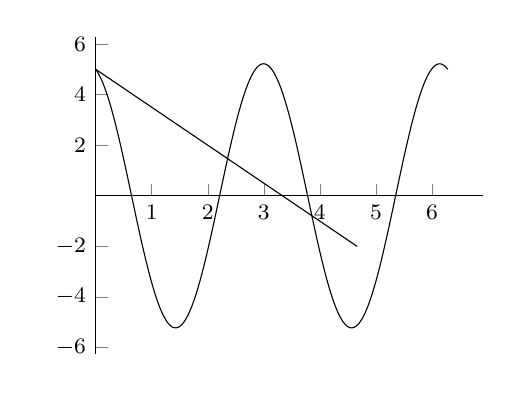
\begin{tikzpicture}
\begin{axis}[small,axis lines*=middle,xmin=0]
\addplot[domain=0:2*pi,samples=200]{5*cos(2*x*180/pi)-1.5*sin(2*x*180/pi)};
\addplot[] plot coordinates {(0,5) (4.666,-2)};
\end{axis}
\end{tikzpicture}
\caption{مثال \حوالہ{مثال_سادہ_دو_درجی_ابتدائی_قیمت_الف} کا جبری حل۔}
\label{شکل_مثال_سادہ_دو_درجی_ابتدائی_قیمت_الف}
\end{figure}
\انتہا{مثال}
%===================

درج بالا مثال میں \عددی{y_1} اور \عددی{y_2} ایسے تفاعل تھے جن سے حاصل عمومی حل ابتدائی معلومات پر پورا اترتا تھا۔آئیں اب دو آپس میں راست تناسب حل لیتے ہوئے عمومی حل  لکھیں، مثلاً \عددی{y_1=\cos 2x} اور \عددی{y_2=k\cos 2x} لیتے ہوئے
\begin{align*}
y=c_1\cos 2x+c_2 k\cos 2x=(c_1+c_2k)\cos 2x=c_3\cos 2x
\end{align*}
عمومی حل لکھتے ہیں۔اس مساوات میں ایک عدد اختیاری مستقل \عددی{c_3} پایا جاتا ہے جو دونوں ابتدائی قیمتوں پر پورا اترنے کے لئے نا کافی ہے۔یوں ہم دیکھتے ہیں کہ عمومی حل لکھتے ہوئے ایسے موزوں حل کا خطی میل لیا جاتا ہے جو آپس میں راست تناسبی نہ ہوں۔

 آپ نے یہ بھی دیکھ لیا ہو گا کہ عمومی حل میں استعمال ہونے والے موزوں حل \عددی{y_1} اور \عددی{y_2} انفرادی طور پر دونوں ابتدائی معلومات پر پورا نہیں اتر سکتے البتہ ان کا خطی میل دونوں ابتدائی معلومات پر پورا اترتا ہے۔یہی عمومی حل کی اہمیت کی وجہ ہے۔
%===========================

\ابتدا{قانون}\quad عمومی حل، اساس اور جبری حل کے تعریف\\
کھلے وقفہ \عددی{I} پر سادہ تفرقی مساوات \حوالہ{مساوات_سادہ_متجانس_دو_درجی_تعریف} کا عمومی حل مساوات \حوالہ{مساوات_سادہ_دو_درجی_عمومی_حل_الف} دیتا ہے جہاں \عددی{I} پر \عددی{y_1} اور \عددی{y_2} مساوات  \حوالہ{مساوات_سادہ_متجانس_دو_درجی_تعریف} کے  (آپس میں) غیر تناسبی حل اور \عددی{c_1}، \عددی{c_2} اختیاری مستقل ہیں۔فاصلہ \عددی{I} پر \عددی{y_1} اور \عددی{y_2} مساوات \حوالہ{مساوات_سادہ_متجانس_دو_درجی_تعریف} کی \اصطلاح{اساس}\فرہنگ{اساس!حل}\حاشیہب{basis}\فرہنگ{basis!of solutions} حل کہلاتے ہیں۔

کھلے وقفہ \عددی{I} پر سادہ تفرقی مساوات \حوالہ{مساوات_سادہ_متجانس_دو_درجی_تعریف} کا جبری حل مساوات \حوالہ{مساوات_سادہ_دو_درجی_عمومی_حل_الف} میں \عددی{c_1} اور \عددی{c_2} کی جگہ مخصوص قیمتیں پر کرنے سے حاصل ہوتا ہے۔
\انتہا{قانون}
%============================

کھلے وقفہ کی تعریف حصہ \حوالہ{حصہ_حل_کا_تصور_سادہ_اول} میں دی گئی ہے۔ \عددی{y_1} اور \عددی{y_2} اس صورت  تناسبی تصور کئے جاتے ہیں  جب پورے \عددی{I} پر
\begin{align}
(a)\quad y_1=ky_2 \quad \text{یا} \quad  (b) \quad y_2=ly_1
\end{align} 
ہو، جہاں \عددی{k} اور \عددی{l} اعداد ہیں جو صفر بھی ہو سکتے ہیں۔(یہاں توجہ رکھیں: \عددی{a} اس صورت \عددی{b} کے مترادف ہے جب \عددی{k \ne 0} ہو۔)

آئیں اساس کی تعریف ذرہ مختلف اور عمومی اہمیت کے حامل طریقے سے بیان کریں۔  وقفہ \عددی{I} پر معین \عددی{y_1} اور \عددی{y_2} اس وقفے پر اس صورت \اصطلاح{خطی طور غیر تابع}\فرہنگ{خطی طور! غیر تابع}\حاشیہب{linearly independent}\فرہنگ{linearly independent} کہلاتے ہیں جب پورے \عددی{I} پر
\begin{align}\label{مساوات_سادہ_دو_درجی_خطی_طور_غیر_تابع_الف}
k_1 y_1+k_2 y_2=0
\end{align}
سے مراد 
\begin{gather}
\begin{aligned}
k_1&=0\\
k_2&=0
\end{aligned}
\end{gather}
ہو۔\عددی{k_1} اور \عددی{k_2} میں سے کم از کم ایک کی قیمت صفر کے برابر نہ ہونے کی صورت میں مساوات \حوالہ{مساوات_سادہ_دو_درجی_خطی_طور_غیر_تابع_الف} پر پورا اترتے ہوئے \عددی{y_1} اور \عددی{y_2} \اصطلاح{خطی طور تابع}\فرہنگ{خطی طور!تابع}\حاشیہب{linearly dependent}\فرہنگ{linearly dependent} کہلاتے ہیں۔اگر \عددی{k_1 \ne 0} ہو تب ہم مساوات \حوالہ{مساوات_سادہ_دو_درجی_خطی_طور_غیر_تابع_الف} کو \عددی{k_1} سے تقسیم کرتے ہوئے \عددی{y_1=\tfrac{k_2}{k_1}y_2} لکھ سکتے ہیں جو تناسبی رشتہ ہے۔اسی طرح \عددی{k_2 \ne 0} کی صورت میں \عددی{y_2=\tfrac{k_1}{k_2}y_1} لکھا جا سکتا ہے جو تناسبی رشتے کو ظاہر کرتی ہے۔اس کے برعکس خطی طور غیر تابع صورت میں ہم مساوات \حوالہ{مساوات_سادہ_دو_درجی_خطی_طور_غیر_تابع_الف} کو \عددی{k_1} (یا \عددی{k_2}) سے تقسیم نہیں کر سکتے لہٰذا  تناسبی رشتہ حاصل نہیں کیا جا سکتا۔ اس طرح اساس کی قدر مختلف تعریف حاصل ہوتی ہے۔
%=====================

\ابتدا{قانون}اساس کی قدر مختلف تعریف\\
کھلے وقفے \عددی{I} پر مساوات \حوالہ{مساوات_سادہ_دو_درجی_خطی_طور_غیر_تابع_الف} کا خطی طور غیر تابع حل   مساوات \حوالہ{مساوات_سادہ_دو_درجی_خطی_طور_غیر_تابع_الف} کے حل کا \اصطلاح{اساس}\فرہنگ{اساس}\فرہنگ{basis} ہے۔
\انتہا{قانون}
%======================

اگر کسی کھلے وقفے \عددی{I} پر  مساوات \عددی{مساوات_سادہ_متجانس_دو_درجی_تعریف} کے  عددی سر \عددی{p} اور \عددی{q} استمراری تفاعل ہوں تب اس وقفے پر مساوات \عددی{مساوات_سادہ_متجانس_دو_درجی_تعریف} کے کا عمومی حل پایا جاتا ہے۔مساوات \حوالہ{مساوات_سادہ_دو_درجی_ابتدائی_قیمتیں} میں دیے ابتدائی معلومات استعمال کرتے ہوئے اس عمومی حل سے  جبری حل حاصل ہو گا۔ وقفہ \عددی{I} پر مساوات  کے تمام حل یہی عمومی مساوات دے گا لہٰذا ایسی صورت میں مساوات کا کوئی \اصطلاح{نادر}\فرہنگ{نادر!حل}\حاشیہب{singular solution}\فرہنگ{singular solution} حل نہیں پایا جاتا (نادر حل کو عمومی حل سے حاصل نہیں کیا جا سکتا ہے۔ یہاں سوال \حوالہ{سوال_سادہ_اول_نادر_حل_الف} سے رجوع کریں)۔ ان تمام حقائق کی وضاحت جلد کی جائے گی۔
%=======================

\ابتدا{مثال}\quad اساس، عمومی اور جبری حل\\
\عددی{\cos 2x} اور \عددی{\sin 2x} تمام \عددی{x} پر مثال \حوالہ{مثال_سادہ_دو_درجی_ابتدائی_قیمت_الف} کے تفرقی مساوات \عددی{y''+4y=0} کے حل کی اساس ہیں۔ایسا اس لئے ہے کہ \عددی{\tfrac{\cos 2x}{\sin 2x} \ne c} اور \عددی{\tfrac{\sin 2x}{\cos 2x} \ne 0} ہیں جہاں \عددی{c} مستقل ہے۔اس مثال میں ابتدائی معلومات استعمال کرتے ہوئے عمومی حل سے جبری حل \عددی{y=5\cos 2x-1.5\sin 2x} حاصل کیا گیا تھا۔
\انتہا{مثال}
%============================
\ابتدا{مثال}
پر کرتے ہوئے ثابت کریں کہ \عددی{y_1=e^{2x}} اور \عددی{y_2=e^{-2x}} سادہ تفرقی مساوات \عددی{y''-4y=0} کے حل ہیں۔یوں درج ذیل ابتدائی قیمت مسئلے کو حل کریں۔
\begin{align*}
y''-4y=0, \quad y(0)=2, \, y'(0)=1
\end{align*}

حل:چونکہ \عددی{y_1''-4y_1=(e^{2x})''-4e^{2x}=4e^{2x}-4e^{2x}=0} اور \عددی{y_2''-4y_2=(e^{-2x})''-4e^{-2x}=4e^{2x}-4e^{2x}=0}  ہیں لہٰذا \عددی{y_1} اور \عددی{y_2} دیے گئے تفرقی مساوات کے حل ہیں۔چونکہ \عددی{\tfrac{e^{2x}}{e^{-2x}} \ne c} ہے جہاں \عددی{c} مستقل کو ظاہر کرتا ہے  لہٰذا دونوں حل غیر متناسب ہیں اور یوں \عددی{e^{2x}} اور \عددی{e^{-2x}} پورے \عددی{x} پر  حل کا  اساس ہے۔اساس کو استعمال کرتے ہوئے عمومی حل لکھتے ہیں۔
\begin{align*}
y=c_1e^{2x}+c_2e^{-2x}
\end{align*}
عمومی حل اور عمومی حل کے تفرق میں ابتدائی قیمتیں پر کرتے ہوئے مستقل \عددی{c_1} اور \عددی{c_2} حاصل کرتے ہیں۔
\begin{align*}
y(0)=c_1e^{0}+c_2e^{0}=c_1+c_2=2, \quad y'=2c_1e^{2x}-2c_2e^{-2x}, \quad y'(0)=2c_1-2c_2=1
\end{align*}
دو عدد ہمزاد مساوات \عددی{c_1+c_2=2} اور \عددی{2c_1-2c_2=1} کو آپس میں حل کرتے ہوئے \عددی{c_1=\tfrac{3}{4}} اور \عددی{c_2=\tfrac{5}{4}} ملتے ہیں جس سے جبری حل لکھا جا سکتا ہے۔
\begin{align*}
y=\frac{3}{4}e^{2x}+\frac{5}{4}e^{-2x}
\end{align*}
\انتہا{مثال}
%=========================

\حصہ{ایک حل معلوم ہونے کی صورت میں اساس دریافت کرنا۔ درجہ کم کرنا}

\باب{بلند درجی خطی سادہ تفرقی مساوات}
دو درجی خطی سادہ تفرقی مساوات کو حل کرنے کے طریقے بلند درجی خطی سادہ ترفقی مساوات کے لئ بھی قابل استعمال ہیں۔ہم دیکھیں گے کہ بلند درجی صورت میں مساوات زیادہ پیچیدہ ہوں گے،  امتیازی مساوات کے جذر بھی تعداد میں زیادہ اور حصول میں نسبتاً مشکل ہوں گے اور ورونسکی زیادہ اہم کردار ادا کرے گا۔ 

\حصہ{متجانس خطی سادہ تفرقی مساوات}
\عددی{n} درجی سادہ تفرقی مساوات سے مراد ایسی مساوات ہے جس میں نا معلوم متغیرہ \عددی{y(x)} کا \عددی{y^n=\tfrac{\dif^{\, n} y}{\dif x^n}} سب سے بلند درجی تفرق ہو۔ایسی سادہ تفرقی مساوات کو
\begin{align*}
F(x,y,y',\cdots, y^{(n)})=0
\end{align*}
لکھا جا سکتا ہے جس میں \عددی{y} اور کم درجی تفرق موجود یا غیر موجود ہو سکتے ہیں۔ایسی مساوات کو \اصطلاح{خطی}\فرہنگ{خطی}\فرہنگ{linear} کہتے ہیں اگر اس کو 
\begin{align}\label{مساوات_سادہ_بلند_خطی_الف}
y^{(n)}+p_{n-1}(x)y^{(n-1)}+\cdots+p_1(x)y'+p_0(x)y=r(x)
\end{align}
لکھنا ممکن ہو۔صفحہ \حوالہصفحہ{مساوات_سادہ_دو_درجی_تعریف} پر دو درجی خطی سادہ تفرقی مساوات کی بات کی گئی۔موجودہ مساوات میں \عددی{n=2}، \عددی{p_1=p} اور \عددی{p_0=q} پر کرنے سے دو درجی مساوات حاصل ہو گی۔عددی سر \عددی{p_0(x)} تا \عددی{p_n(x)}  اور جبری تفاعل \عددی{r(x)} غیر تابع متغیرہ  \عددی{x} کے کوئی بھی تفاعل ہو سکتے ہیں جبکہ \عددی{y(x)} نا معلوم متغیرہ ہے۔خطی مساوات کو معیاری صورت میں لکھا گیا ہے جہاں \عددی{y^{(n)}} کا عددی سر اکائی \عددی{1} ہے۔ تفرقی مساوات میں  \عددی{p_n(x)y^{(n)}} موجود ہونے کی صورت میں پوری مساوات کو \عددی{p_n(x)} سے تقسیم کرتے ہوئے معیاری صورت حاصل کریں۔جو تفرقی مساوات درج بالا صورت میں لکھنا ممکن نہ ہو \اصطلاح{غیر خطی}\فرہنگ{غیر خطی}\فرہنگ{non linear} کہلاتی ہے۔

کسی کھلے وقفے \عددی{I} پر \عددی{r(x)} \اصطلاح{مکمل صفر}\فرہنگ{مکمل صفر} \عددی{r \equiv 0} ہونے کی صورت میں  مساوات \حوالہ{مساوات_سادہ_بلند_خطی_الف} سے \اصطلاح{متجانس مساوات}\فرہنگ{متجانس مساوات}\فرہنگ{homogeneous}
\begin{align}\label{مساوات_سادہ_بلند_خطی_ب}
y^{(n)}+p_{n-1}(x)y^{(n-1)}+\cdots+p_1(x)y'+p_0(x)y=0
\end{align}
حاصل ہوتی ہے۔کھلے وقفے پر \عددی{r(x)} کے مکمل صفر ہونے سے مراد یہ ہے کہ اس وقفے پر ہر \عددی{x} کے لئے \عددی{r(x)} کی قیمت صفر کے برابر ہے۔دو درجی تفرقی مساوات کی طرح  اگر \عددی{r(x)} مکمل صفر نہ ہو تب مساوات \اصطلاح{غیر متجانس}\فرہنگ{غیر متجانس}\فرہنگ{nonhomogeneous} کہلائے گی۔

کھلے وقفہ \عددی{I} پر \عددی{n} درجی خطی یا غیر خطی سادہ تفرقی مساوات کے حل \عددی{y=h(x)} سے مراد ایسا تفاعل ہے جو \عددی{I} پر معین ہو،  کھلے وقفے پر اس کا \عددی{n} درجی تفرق موجود ہو اور تفرقی مساوات میں \عددی{y} اور اس کے تفرقات کی جگہ \عددی{h} اور اس کے تفرقات پر کرنے سے مساوات کے دونوں اطراف بالکل یکساں حاصل ہوں۔ 
%=======================

\جزوحصہء{متجانس خطی سادہ تفرقی مساوات:خطی میل اور عمومی حل}
\اصطلاح{خطی میل}\فرہنگ{خطی میل} یا \اصطلاح{اصول خطیت}\فرہنگ{اصول خطیت} جس کا ذکر صفحہ \حوالہصفحہ{مسئلہ_دو_درجی_خطی_میل} مسئلہ \حوالہ{مسئلہ_دو_درجی_خطی_میل} میں کیا گیا بلند درجی خطی متجانس سادہ تفرقی مساوات کے لئے بھی درست ہے۔
%===============

\ابتدا{مسئلہ}\quad بنیادی مسئلہ برائے متجانس خطی سادہ بلند درجی تفرقی مساوات\فرہنگ{مسئلہ!بنیادی۔متجانس خطی}\\
کھلے وقفہ \عددیء{I} پر متجانس خطی بلند درجی تفرقی مساوات \حوالہ{مساوات_سادہ_بلند_خطی_ب} کے حل کا خطی میل بھی \عددیء{I} پر اس مساوات کا حل ہو گا۔بالخصوص ان حل کو مستقل مقدار سے ضرب دینے سے بھی مساوات کے حل حاصل ہوتے ہیں۔(یہ اصول غیر خطی اور  غیر متجانس مساوات پر لاگو نہیں ہوتا۔)
\انتہا{مسئلہ}
%==========================

اس کا ثبوت گزشتہ باب میں دئے گئے ثبوت کی طرح ہے جس کو یہاں پیش نہیں کیا جائے گا۔

ہماری بقایا گفتگو ہو بہو دو درجی تفرقی مساوات کی طرح ہو گی لہٰذا یہاں بلند درجی خطی متجانس مساوات کی عمومی حل کی بات کرتے ہیں۔ایسا کرنے کی خاطر \عددی{n} عدد تفاعل کی  \اصطلاح{خطی طور غیر تابع}\فرہنگ{غیر تابع!خطی طور}\فرہنگ{خطی طور!غیر تابع} ہونے کی تصور کو وسعت دیتے ہیں۔

%====================
\ابتدا{تعریف}\quad عمومی حل، اساس اور مخصوص حل\\
کھلے وقفے \عددی{I} پر مساوات \حوالہ{مساوات_سادہ_بلند_خطی_ب} کا \اصطلاح{عمومی حل}\فرہنگ{عمومی حل}\فرہنگ{general solution}
\begin{align}
y(x)=c_1y_1(x)+c_2y_2(x)+\cdots +c_ny_n(x)
\end{align}
ہے جہاں \عددی{y_1(x)} تا \عددی{y_n(x)} حل کی اساس اور \عددی{c_1} تا \عددی{c_2} اختیاری مستقل ہیں۔یوں \عددی{y_1} تا \عددی{y_n} کھلے وقفے پر خطی طور غیر تابع ہیں۔ 

عمومی حل کے مستقل کی قیمتیں مقرر کرنے سے \اصطلاح{مخصوص حل}\فرہنگ{مخصوص حل}\فرہنگ{particular solution} حاصل ہو گا۔
\انتہا{تعریف}
%=========================

\ابتدا{تعریف}\quad خطی طور تابع تفاعل اور خطی طور غیر تابع تفاعل\\
تصور کریں کہ کھلے وقفے \عددی{I} پر  \عددی{n} عدد تفاعل \عددی{y_1(x)} تا \عددی{y_n(x)} معین ہیں۔

 وقفہ \عددی{I} پر معین \عددی{y_1} تا \عددی{y_n}،  اس وقفے   پر اس صورت \اصطلاح{خطی طور غیر تابع}\فرہنگ{خطی طور! غیر تابع}\حاشیہب{linearly independent}\فرہنگ{linearly independent} کہلاتے ہیں جب پورے وقفے پر
\begin{align}\label{مساوات_سادہ_بلند_خطی_طور_غیر_تابع_الف}
k_1 y_1(x)+k_2 y_2(x)+\cdots+k_ny_n(x)=0
\end{align}
سے مراد 
\begin{align*}
k_1=k_2= \cdots =k_n=0 
\end{align*}
ہو۔\عددی{k_1} تا \عددی{k_n} میں  کم از کم ایک کی قیمت صفر نہ ہونے کی صورت میں مساوات \حوالہ{مساوات_سادہ_بلند_خطی_طور_غیر_تابع_الف} پر پورا اترتے ہوئے حل \عددی{y_1} تا \عددی{y_n} \اصطلاح{خطی طور تابع}\فرہنگ{خطی طور!تابع}\حاشیہب{linearly dependent}\فرہنگ{linearly dependent} کہلاتے ہیں۔
\انتہا{تعریف}
%==========================

\عددی{y_1} تا \عددی{y_n} میں (کم از کم ایک) تفاعل کو اس صورت بقایا تفاعل کے \اصطلاح{خطی میل}\فرہنگ{خطی میل} کے طرز پر لکھا جا سکتا ہے جب اس وقفے پر \عددی{y_1} تا \عددی{y_n} خطی طور تابع ہوں۔ یوں اگر \عددی{k_1 \ne 0} ہو تب ہم مساوات \حوالہ{مساوات_سادہ_بلند_خطی_طور_غیر_تابع_الف} کو \عددی{k_1} سے تقسیم کرتے ہوئے
\begin{align*}
y_1=-\frac{1}{k_1}(k_2 y_2+k_3y_3+\cdots+k_ny_n)
\end{align*}
 لکھ سکتے ہیں جو تناسبی رشتہ ہے۔یہ مساوات کہتی ہے کہ \عددی{y_1} کو بقایا تفاعل کے خطی میل کی صورت میں لکھا جا سکتا ہے۔اسی کو خطی طور تابع کہتے ہیں۔آپ دیکھ سکتے ہیں کہ \عددی{n=2} کی صورت میں ہمیں حصہ \حوالہ{حصہ_سادہ_دو_وجودیت_یکتائی_ورونسکی} میں بیان کئے گئے تصورات ملتے ہیں۔
%=======================

\ابتدا{مثال}\quad خطی طور تابع\\
ثابت کریں کہ تفاعل \عددی{y_1=2\sin x}، \عددی{y_2=1.5x^2}، \عددی{y_3=5\cos x+\sin x} اور \عددی{y_4=4\cos x} کسی بھی کھلے وقفے پر خطی طور تابع ہیں۔

حل:ہم \عددی{y_3=\tfrac{1}{2}y_1+0y_2+\tfrac{5}{4}y_4} لکھ سکتے ہیں لہٰذا \عددی{y_1} تا \عددی{y_4} خطی طور تابع تفاعل ہیں۔
\انتہا{مثال}
%============================
\ابتدا{مثال}\شناخت{مثال_سادہ_بلند_خطی_طور_غیر_تابع}\quad خطی طور غیر تابع\\
ثابت کریں کہ \عددی{y_1=x}، \عددی{y_2=x^3} اور \عددی{y=x^4}  کسی بھی کھلے وقفے پر خطی طور غیر تابع ہیں۔

حل:ہم  مساوات \عددی{k_1y_1+k_2y_2+k_3y_3=0} میں مختلف \عددی{x} کی قیمتیں پر کرتے ہوئے \عددی{k_1} تا \عددی{k_3} دریافت کرتے ہیں۔کھلے وقفے پر نقطہ \عددی{x=1}، \عددی{x=-1} اور \عددی{x=2} چنتے ہوئے درج ذیل ہمزاد مساوات ملتے ہیں۔
\begin{align*}
k_1+k_2+k_3&=0\\
-k_1-k_2+k_3&=0\\
2k_1+8k_2+16k_3&=0
\end{align*}
ان ہمزاد مساوات کو حل کرتے ہوئے \عددی{k_1=0}، \عددی{k_2=0} اور \عددی{k_3=0} ملتا ہے جو خطی طور غیر تابع ہونے کا ثبوت ہے۔
\انتہا{مثال}
%========================
\ابتدا{مثال}\شناخت{مثال_سادہ_بلند_اساس_عمومی_حل_الف}\quad اساس۔عمومی حل\\
تین درجی سادہ تفرقی مساوات \عددی{y^{(3)}-y'=0} کا عمومی حل تلاش کریں۔ \عددی{y^{(3)}} سے مراد \عددی{\tfrac{\dif^{\,3} y}{\dif x^3}} ہے۔

حل:حصہ \حوالہ{حصہ_سادہ_دو_درجی_مستقل_عددی_سر} کی طرح ہم اس متجانس مساوات کا حل \عددی{y=e^{\lambda x}} تصور کرتے  ہوئے امتیازی مساوات
\begin{align*}
\lambda^3-\lambda=0
\end{align*}
حاصل کرتے ہیں۔اس کو \عددی{\lambda(\lambda^2-1)=0} لکھتے ہوئے \عددی{\lambda=0} اور \عددی{\lambda=\mp 1} ملتے ہیں جن سے اساس \عددی{y_1=c}، \عددی{y_2=e^x} اور \عددی{y_3=e^{-x}} ملتا ہے۔جیسا مثال \حوالہ{مثال_سادہ_بلند_اساس_عمومی_حل_ب} میں ثابت کیا جائے گا، یہ اساس کسی بھی کھلے وقفے پر خطی طور غیر تابع ہیں لہٰذا کسی بھی کھلے وقفے پر  عمومی حل 
\begin{align*}
y=c_1+c_2e^x+c_3e^{-x}
\end{align*}
ہو گا۔
\انتہا{مثال}
%=======================

\جزوحصہء{ابتدائی قیمت مسئلہ۔وجودیت اور یکتائی}
مساوات \حوالہ{مساوات_سادہ_بلند_خطی_ب} پر مبنی ابتدائی قیمت مسئلہ مساوات \حوالہ{مساوات_سادہ_بلند_خطی_ب} اور درج ذیل \عددی{n} \اصطلاح{ابتدائی شرائط}\فرہنگ{ابتدائی!شرائط} پر مشتمل ہو گا
\begin{align}\label{مساوات_سادہ+بلند_ابتدائی_شرائط}
y(x_0)=K_0, y'(x_0)=K_1,\cdots , y^{(n-1)}(x_0)=K_{n-1}
\end{align}
جہاں \عددی{x_0} کھلے وقفے \عددی{I} پر ایک نقطہ اور \عددی{K_0} تا \عددی{K_{n-1}} اس نقطے پر  دیے گئے مقدار ہیں۔

صفحہ \حوالہصفحہ{مسئلہ_سادہ_دو_درجی_یکتا_مخصوص_حل} پر مسئلہ \حوالہ{مسئلہ_سادہ_دو_درجی_یکتا_مخصوص_حل} کو وسعت دیتے ہیں جس سے درج ذیل ملتا ہے۔
%============================

\ابتدا{مسئلہ}\شناخت{مسئلہ_سادہ_بلند_درجی_یکتا_مخصوص_حل}\quad مسئلہ وجودیت اور یکتائی برائے ابتدائی قیمت بلند درجی  تفرقی مساوات\فرہنگ{مسئلہ!وجودیت اور یکتائی}\\
کھلے وقفہ \عددی{I} پر مساوات \حوالہ{مساوات_سادہ_بلند_خطی_ب} کے عددی سر \عددی{p_0} تا \عددی{p_{n-1}} استمراری ہونے کی صورت میں اگر \عددی{x_0} کھلے وقفے پر پایا جاتا ہو تب مساوات \حوالہ{مساوات_سادہ_بلند_خطی_ب} اور مساوات \حوالہ{مساوات_سادہ+بلند_ابتدائی_شرائط} پر مبنی ابتدائی قیمت مسئلے کا \عددی{I} پر  \اصطلاح{یکتا حل}\فرہنگ{یکتا حل} \عددی{y(x)} \اصطلاح{موجود}\فرہنگ{حل!موجود}\فرہنگ{موجود!حل} ہے۔
\انتہا{مسئلہ}
%============================

حل کی موجودگی اور یکتائی کا ثبوت اس کتاب میں نہیں دیا جائے گا۔

%================
\ابتدا{مثال}\quad تین درجی یولر کوشی مساوات کا ابتدائی قیمت مسئلہ\\
درج ذیل ابتدائی قیمت مسئلے کو حل کریں۔
\begin{align*}
x^3y'''-5x^2y''+12xy'-12y=0,\quad y(1)=1, \quad y'(1)=-1, \quad y''(1)=0
\end{align*}

حل:ہم تفرقی مساوات میں آزمائشی تفاعل \عددی{y=x^m} پر کرتے ہوئے امتیازی مساوات
\begin{align*}
m^3-8m^2+19m-12=0
\end{align*}
حاصل کرتے ہیں جس کے جذر \عددی{m=1}، \عددی{m=3} اور \عددی{m=4} ہیں۔جذر  کو مختلف طریقوں سے حاصل کیا جاتا ہے البتہ یہاں جذر حاصل کرنے پر بحث نہیں کی جائے گی۔ یوں حل کی اساس \عددی{y_1=x}، \عددی{y_2=x^3} اور \عددی{y_3=x^4} ہیں جنہیں مثال \حوالہ{مثال_سادہ_بلند_خطی_طور_غیر_تابع} میں خطی طور غیر تابع ثابت کیا گیا۔اس طرح عمومی حل
\begin{align*}
y=c_1x+c_2x^3+c_3x^4
\end{align*}
ہو گا۔دیے گئے تفرقی مساوات کو  \عددی{x^3} سے تقسیم کرتے ہوئے \عددی{y'''} کا عددی سر اکائی حاصل کرتے ہوئے تفرقی مساوات کی معیاری صورت حاصل ہوتی ہے۔معیاری صورت میں مساوات کے دیگر عددی سر \عددی{x=0} پر غیر استمراری ہیں۔اس کے باوجود درج بالا عمومی حل تمام \عددی{x} بشمول  \عددی{x=0} کے لئے درست ہے۔ 

عمومی حل اور اس کے تفرقات \عددی{y'=c_1+3c_2x^2+4c_3x^3} اور \عددی{y''=6c_2x+12c_3x^2} میں ابتدائی معلومات پر کرتے ہوئے درج ذیل ہمزاد مساوات ملتے ہیں
\begin{align*}
c_1+c_2+c_3&=1\\
c_1+3c_2+4c_3&=-1\\
6c_2+12c_3&=0
\end{align*}
جن کا حل \عددی{c_1=3}، \عددی{c_2=-4} اور \عددی{c_3=2} ہے۔اس طرح مخصوص حل درج ذیل ہو گا۔
\begin{align*}
y=3x-4x^3+2x^4
\end{align*}
\انتہا{مثال}
%==========================

\جزوحصہء{خطی طور غیر تابع حل۔ورونسکی}
عمومی حل کے حصول کے لئے ضروری ہے کہ حل خطی طور غیر تابع ہوں۔اگرچہ عموماً حل کو دیکھ کر ہی اندازہ ہو جاتا ہے کہ  وہ خطی طور غیر تابع ہیں یا نہیں ہیں، البتہ ایسا معلوم کرنے کا منظم طریقہ زیادہ بہتر ہو گا۔صفحہ \حوالہصفحہ{مسئلہ_سادہ_دو_حل_تابع_غیر_تابع} پر مسئلہ \حوالہ{مسئلہ_سادہ_دو_حل_تابع_غیر_تابع} دو درجی  \عددی{n=2} مساوات کے علاوہ بلند درجی مساوت کے لئے بھی درست ہے۔ بلند درجی مساوات کی صورت میں ورونسکی درج ذیل ہو گی۔
\begin{align}\label{مساوات_سادہ_بلند_ورونسکی_الف}
W(y_1,\cdots, y_n)=
\begin{vmatrix}
y_1 & y_2 & \cdots & y_n\\
y'_1 & y'_2 & \cdots & y'_n\\
\vdots & & \\
y_1^{(n-1)} & y_2^{(n-1)} & \cdots & y_n^{(n-1)}
\end{vmatrix}
\end{align}
ورونسکی تفرقی مساوات کے حل \عددی{y_1} تا \عددی{y_n} پر مبنی ہے جو از خود \عددی{x} پر مبنی ہیں۔ورونسکی غیر صفر ہونے کی صورت میں  \عددی{y_1} تا \عددی{y_n} خطی طور غیر تابع ہوں گے۔
%========================

\ابتدا{مسئلہ}\شناخت{مسئلہ_سادہ_بلند_حل_تابع_غیر_تابع}\quad خطی طور تابع اور غیر تابع حل\فرہنگ{مسئلہ!تابع اور غیر تابع حل}\\
کھلے وقفہ \عددی{I} پر استمراری  \عددی{p_0(x)} تا  \عددی{p_{n-1}(x)} عددی سر والے سادہ تفرقی  مساوات \حوالہ{مساوات_سادہ_بلند_خطی_ب} کے \عددی{I}  پر حل \عددی{y_1} تا \عددی{y_n} اس صورت \اصطلاح{خطی طور تابع}\فرہنگ{خطی طور تابع}\فرہنگ{linearly dependent} ہوں گے جب ان کے \اصطلاح{ورونسکی}\فرہنگ{ورونسکی}\حاشیہب{Wronskian}\فرہنگ{Wronskian} کی قیمت  کسی \عددی{x_0} پر صفر کے برابر  ہو، جہاں \عددی{x_0} کھلے وقفے \عددی{I} پر پایا جاتا ہے۔مزید اگر  نقطہ \عددی{x=x_0} پر \عددی{W=0} ہو تب پورے \عددی{I} پر \عددی{W} \اصطلاح{مکمل صفر}\فرہنگ{مکمل صفر}\فرہنگ{صفر!مکمل}\حاشیہب{identically zero}\فرہنگ{identically zero} ہو گا۔یوں اگر \عددی{I} پر کوئی ایسا \عددی{x} پایا جاتا ہو جس پر \عددی{W} صفر کے برابر نہ ہو تب \عددی{I} پر  \عددی{y_1} تا \عددی{y_n} \اصطلاح{خطی طور غیر تابع}\فرہنگ{خطی طور غیر تابع}\فرہنگ{linearly independent} ہوں گے  اور یہ حل کی اساس ہوں گے۔
\انتہا{مسئلہ}
%==============================

\ابتدا{ثبوت}

(الف) \quad تصور کریں کہ کھلے وقفہ \عددی{I} پر  \عددی{y_1} تا \عددی{y_n} مساوات \حوالہ{مساوات_سادہ_بلند_خطی_ب} کے حل ہیں۔یوں خطی طور غیر تابع کی تعریف سے 
\begin{align}\label{مساوات_سادہ_بلند_ورونسکی_ب}
k_1y_1+k_2y_2+\cdots+k_ny_n=0
\end{align}
لکھا جا سکتا ہے۔ \عددی{I} پر اس مساوات کی \عددی{n-1} تفرقات لیتے ہیں۔
\begin{gather}
\begin{aligned}\label{مساوات_سادہ_بلند_ورونسکی_پ}
k_1y'_1+k_2y'_2+\cdots+k_ny'_n&=0\\
k_1y''_1+k_2y''_2+\cdots+k_ny''_n&=0\\
\vdots &\\
k_1y^{(n-1)}_1+k_2y^{(n-1)}_2+\cdots+k_ny^{(n-1)}_n&=0
\end{aligned}
\end{gather}
مساوات \حوالہ{مساوات_سادہ_بلند_ورونسکی_ب} اور مساوات \حوالہ{مساوات_سادہ_بلند_ورونسکی_پ} \عددی{n} عدد خطی متجانس ہمزاد  الجبرائی مساوات کا نظام ہے جس کا \اصطلاح{غیر صفر حل}\فرہنگ{غیر صفر حل}\فرہنگ{حل!غیر صفر}\حاشیہب{non trivial solution}\فرہنگ{non trivial solution} \عددی{k_1} تا \عددی{k_n} ہے لہٰذا \عددی{I} پر تمام \عددی{x} کے لئے، اس نظام کی عددی سر قالب کی حتمی قیمت، \اصطلاح{مسئلہ کریمر}\فرہنگ{مسئلہ!کریمر}\فرہنگ{کریمر!مسئلہ}\حاشیہب{Cramer's theorem}\فرہنگ{Cramer's!theorem} [جسے باب-7 میں پیش کیا گیا ہے] کے تحت ،  صفر کے برابر ہو گی۔اب قالب کی حتمی قیمت ہی ورونسکی ہے لہٰذا \عددی{I} پر تمام \عددی{x} کے لئے \عددی{W} صفر کے برابر ہے۔

(ب) \quad مسئلہ کریمر کو استعمال کرتے ہوئے ہم یوں بھی کہہ سکتے ہیں کہ \عددی{W=0} کی صورت میں مساوات \حوالہ{مساوات_سادہ_بلند_ورونسکی_ب} اور مساوات \حوالہ{مساوات_سادہ_بلند_ورونسکی_پ} خطی متجانس ہمزاد  الجبرائی مساوات کے نظام کا \عددی{x=x_0} پر غیر صفر حل \عددی{k^*_1} تا \عددی{k^*_n} پایا جاتا ہے جس کو استعمال کرتے ہوئے، \عددی{I} پر مساوات \حوالہ{مساوات_سادہ_بلند_خطی_ب} کا عمومی حل\عددی{y^*=k^*_1y_1+\cdots+k^*_ny_n} لکھا جا سکتا ہے۔مساوات \حوالہ{مساوات_سادہ_بلند_ورونسکی_ب} اور مساوات \حوالہ{مساوات_سادہ_بلند_ورونسکی_پ}  کے تحت  \عددی{y^*} ابتدائی شرائط \عددی{y^*(x_0)=0} تا \عددی{y^{*(n-1)}(x_0)=0} پر پورا اترتا ہے۔انہیں ابتدائی شرائط پر حل \عددی{y \equiv 0} بھی پورا اترتا ہے اور یوں مسئلہ \حوالہ{مسئلہ_سادہ_بلند_درجی_یکتا_مخصوص_حل} کے تحت، چونکہ  مساوات \حوالہ{مساوات_سادہ_بلند_ورونسکی_ب} کے عددی سر \عددی{I} پر استمراری ہیں، لہٰذا \عددی{y^*=y} ہو گا۔اس طرح \عددی{y^*=k^*_1y_1+\cdots+k^*_ny_n \equiv 0} پورے \عددی{I} پر ہو گا جس کا مطلب ہے کہ  \عددی{I} پر \عددی{y_1} تا \عددی{y_n} خطی طور تابع ہیں۔

(پ)\quad اگر \عددی{W} کی قیمت \عددی{x_0} پر صفر ہو جہاں \عددی{x_0} کھلے وقفہ \عددی{I} پر پایا جاتا ہو، تب ثبوت (ب) کے تحت خطی طور تابع ہونا ثابت ہوتا ہے اور یوں ثبوت (الف) کے تحت \عددی{W \equiv 0} ہو گا۔اس طرح اگر \عددی{I} پر نقطہ \عددی{x_1} پر \عددی{W} صفر نہ ہو تب \عددی{y_1} تا \عددی{y_n} کھلے وقفہ \عددی{I} پر خطی طور غیر تابع ہوں گے۔
\انتہا{ثبوت}
%============================

\ابتدا{مثال}\شناخت{مثال_سادہ_بلند_اساس_عمومی_حل_ب} \quad اساس۔ ورونسکی\\
ثابت کریں کہ مثال \حوالہ{مثال_سادہ_بلند_اساس_عمومی_حل_الف} میں حاصل کردہ حل \عددی{y_1=c}، \عددی{y_2=e^x} اور \عددی{y_3=e^{-x}} خطی طور غیر تابع ہیں۔

حل: مساوات \حوالہ{مساوات_سادہ_بلند_ورونسکی_الف} کے طرز پر  ورونسکی لکھ ک
\begin{align*}
W=
\begin{vmatrix}
c& e^x& e^{-x}\\
0& e^x & -e^{-x}\\
0&e^x&e^x
\end{vmatrix}
=c e^{x} e^{-x}
\begin{vmatrix}
1& 1& 1\\
0& 1 & -1\\
0&1&1
\end{vmatrix}=
c
\begin{vmatrix}
1& -1\\
1&1
\end{vmatrix}
=2c
\end{align*}
حل کیا گیا ہے جہاں پہلی قطار سے \عددی{c}، دوسری قطار سے \عددی{e^x} اور تیسری قطار سے \عددی{e^{-x}} باہر نکال کر قالب کی سادہ صورت حاصل کی گئی اور اس کے بعد پہلی قطار سے قالب کو پھیلا کر اس کی حتمی قیمت حاصل کی گئی ہے۔چونکہ \عددی{x} کی کسی بھی قیمت کے لئے  \عددی{W \ne 0} ہے لہٰذا کسی بھی کھلے وقفے پر \عددی{y_1} تا \عددی{y_3} خطی طور غیر تابع ہیں۔
\انتہا{مثال}
%========================

\جزوحصہء{مساوات \حوالہ{مساوات_سادہ_بلند_خطی_ب} کے عمومی حل میں تمام حل شامل ہیں}

\باب{نظامِ تفرقی مساوات}
گزشتہ باب میں آپ نے بلند رتبی سادہ تفرقی مساوات کو حل کرنا سیکھا۔اس باب میں سادہ تفرقی مساوات کو حل کرنے کا نیا طریقہ دکھایا جائے گا جس میں \عددی{n} رتبی سادہ تفرقی مساوات سے \عددی{n} عدد یک رتبی سادہ تفرقی مساوات کا نظام حاصل کیا جائے گا۔اس نظام کو حل کرنا بھی سکھایا جائے گا۔تفرقی مساوات کے نظام کو قالب اور سمتیہ کی صورت میں لکھنا زیادہ مفید ثابت ہوتا ہے لہٰذا حصہ \حوالہ{حصہ_نظام_قالب} میں قالب اور سمتیہ کے بنیادی حقائق پر غور کیا جائے گا۔

اسی باب میں تفرقی مساوات کے نظام کو حل کرنے کی بجائے تمام مساوات کے مجموعی طرز عمل پر غور کیا جائے گا جس سے نظام کے حل کے \اصطلاح{استحکام}\فرہنگ{استحکام}\حاشیہب{stability}\فرہنگ{stability} کے بارے میں معلومات حاصل ہوتی ہے۔انجینئری میں مستحکم نظام  اہمیت رکھتے ہیں۔مستحکم نظام میں کسی لمحے پر معمولی تبدیلی، مستقبل کے لمحات پر معمولی تبدیلی ہی پیدا کرتی ہے۔اس ترکیب سے مساوات کا اصل حل دریافت نہیں ہوتا لہٰذا اس کو \اصطلاح{کیفی ترکیب}\فرہنگ{کیفی ترکیب}\فرہنگ{ترکیب!کیفی}\حاشیہب{qualitative method}\فرہنگ{qualitative method} کہتے ہیں۔جس ترکیب سے نظام کا اصل حل حاصل ہوتا ہو اس کو \اصطلاح{مقداری ترکیب}\فرہنگ{مقداری ترکیب}\فرہنگ{ترکیب!مقداری}\حاشیہب{quantitative method}\فرہنگ{quantitative method} کہتے ہیں۔

 
\حصہ{قالب اور سمتیہ کے بنیادی حقائق}\شناخت{حصہ_نظام_قالب}
تفرقی مساوات کے نظام پر غور کے دوران قالب اور سمتیات استعمال کئے جائیں گے۔

دو عدد خطی سادہ تفرقی مساوات کے نظام
\begin{gather}\label{مساوات_نظام_دو_مساوات}
\begin{aligned}
y_1' &=a_{11}y_1+a_{12}y_2\\
y_2' &=a_{21}y_1+a_{22}y_2
\end{aligned}\quad \text{یا} \quad
\begin{aligned}
y_1' &=2y_1-7y_2\\
y_2' &=5y_1+y_2
\end{aligned}
\end{gather}
 میں دو عدد نا معلوم تفاعل \عددی{y_1(t)} اور \عددی{y_2(t)} پائے جاتے ہیں۔ان مساوات میں دائیں جانب اضافی تفاعل \عددی{g_1(t)} اور \عددی{g_2(t)} بھی موجود ہو سکتے ہیں۔اسی طرح \عددی{n} عدد یک رتبی سادہ تفرقی مساوات پر مبنی نظام
\begin{gather}
\begin{aligned}\label{مساوات_نظام_متعدد_مساوات}
y_1' &=a_{11}y_1+a_{12}y_2+\cdots+a_{1n}y_n\\
y_2' &=a_{21}y_1+a_{22}y_2+\cdots a_{2n}y_n\\
\vdots &\\
y_n'&=a_{n1}y_1+a_{n2}y_2+\cdots+a_{nn}y_n
\end{aligned}
\end{gather}
 میں \عددی{y_1(t)} تا \عددی{y_n(t)} نا معلوم تفاعل پائے جائیں گے۔درج بالا ہر مساوات میں دائیں جانب اضافی تفاعل بھی پائے جا سکتے ہیں۔
%====================
\جزوحصہء{تکنیکی اصطلاحات}
\جزوحصہء{قالب}
نظام \حوالہ{مساوات_نظام_دو_مساوات} کے عددی سر (جو مستقل یا متغیرات ممکن ہیں) کو \عددی{2 \times 2} \اصطلاح{قالب}\فرہنگ{قالب}\حاشیہب{matrix}\فرہنگ{matrix} \bM{A} کی صورت میں لکھا جا سکتا ہے۔
\begin{gather}\label{مساوات_نظام_دو_جمع_دو_قالب}
\begin{aligned}
\bM{A}=[a_{jk}]=
\begin{bmatrix*}[r]
a_{11} & a_{12}\\
a_{21} & a_{22}
\end{bmatrix*}
\end{aligned}\quad \text{یا} \quad
\begin{aligned}
\bM{A}=[a_{jk}]=
\begin{bmatrix*}[r]
3 & 2\\
-1 &\frac{2}{3}
\end{bmatrix*}
\end{aligned}
\end{gather}
اسی طرح نظام \حوالہ{مساوات_نظام_متعدد_مساوات} کے عددی سر کو \عددی{n \times n} قالب کی صورت میں لکھا جا سکتا ہے۔
\begin{align}\label{مساوات_نظام_متعدد_جمع_متعدد_قالب}
\bM{A}=[a_{jk}]=
\begin{bmatrix*}[r]
a_{11} & a_{12} &\cdots & a_{1n}\\
a_{21} & a_{22}& \cdots & a_{2n}\\
& \vdots &  &\\
a_{n1} & a_{n2}& \cdots & a_{nn}
\end{bmatrix*}
\end{align}
قالب میں درج \عددی{a_{11}}، \عددی{a_{12}}، \عددی{a_{21}} وغیرہ کو \اصطلاح{ارکان}\فرہنگ{ارکان}\حاشیہب{entry}\فرہنگ{entry} کہتے ہیں۔ افقی لکیروں کو \اصطلاح{صف}\فرہنگ{صف}\حاشیہب{row}\فرہنگ{row} جبکہ عمودی لکیروں کو \اصطلاح{قطار}\فرہنگ{قطار}\حاشیہب{column}\فرہنگ{column} کہتے ہیں۔قالب \حوالہ{مساوات_نظام_دو_جمع_دو_قالب} میں پہلا صف \عددی{[a_{11} \,\,\,  a_{12}]} یا \عددی{[3\,\,\, 2]} جبکہ دوسرا صف \عددی{[a_{21} \,\,\,  a_{22}]} یا \عددی{[-1\,\,\,\tfrac{2}{3}]} ہے۔اسی طرح پہلا قطار درج ذیل ہے۔
\begin{gather*}
\begin{aligned}
\begin{bmatrix*}[r]
a_{11}\\
a_{21}
\end{bmatrix*}\quad \text{یا}\quad 
\begin{bmatrix*}[r]
3\\
-1
\end{bmatrix*}
\end{aligned}
\end{gather*}
ارکان کی علامتی اظہار میں دو گنا زیر نوشت کا پہلا عدد صف کو ظاہر کرتا ہے جبکہ دوسرا عدد قطار کو ظاہر کرتا ہے۔یوں \عددی{a_{21}} دوسری صف اور پہلی قطار کا رکن ہے۔ قالب \حوالہ{مساوات_نظام_دو_جمع_دو_قالب} کا \اصطلاح{مرکزی وتر}\فرہنگ{مرکزی وتر}\فرہنگ{وتر!مرکزی}\حاشیہب{main diagonal}\فرہنگ{diagonal!main} \عددی{a_{11}} اور \عددی{a_{22}} پر مبنی ہے جبکہ قالب \حوالہ{مساوات_نظام_متعدد_جمع_متعدد_قالب} کا مرکزی وتر \عددی{a_{11}}، \عددی{a_{22}}، \نقطے، \عددی{a_{nn}} پر مبنی ہے۔ہمیں یہاں صرف \اصطلاح{مربع قالب}\فرہنگ{مربع قالب}\فرہنگ{قالب!مربع}\حاشیہب{square matrix}\فرہنگ{matrix!square} درکار ہوں گے۔مربع قالب سے مراد ایسا قالب ہے جس میں صفوں کی تعداد قطاروں کی تعداد کے برابر ہو۔ قالب \حوالہ{مساوات_نظام_دو_جمع_دو_قالب} اور قالب \حوالہ{مساوات_نظام_متعدد_جمع_متعدد_قالب} مربع قالب ہیں۔

\اصطلاح{سمتیہ}۔\quad ایک قطار اور \عددی{n} ارکان کا \اصطلاح{سمتیہ قطار}\فرہنگ{سمتیہ!قطار}\فرہنگ{قطار!سمتیہ}\حاشیہب{column vector}\فرہنگ{vector!column} درج ذیل ہے۔
\begin{align*}
\bM{x}=
\begin{bmatrix*}[r]
x_1\\
x_2\\
x_3\\
\vdots\\
x_n
\end{bmatrix*}
\end{align*}
اسی طرح ایک صف اور \عددی{n} ارکان کا \اصطلاح{سمتیہ صف}\فرہنگ{سمتیہ صف}\فرہنگ{سمتیہ!صف}\حاشیہب{row vector}\فرہنگ{vector!row} درج ذیل ہے۔
\begin{align*}
\bM{v}=
\begin{bmatrix*}[r]
v_1 & v_2& v_3& \cdots & v_n
\end{bmatrix*}
\end{align*}
%=========================
\جزوحصہء{قالب اور سمتیات کا حساب}
\جزوحصہء{برابری مساوات} دو عدد \عددی{n \times n} قالب صرف اور صرف اس صورت برابر ہوں گے جب ان کے تمام \اصطلاح{مطابقتی}\فرہنگ{مطابقتی}\حاشیہب{corresponding}\فرہنگ{corresponding} ارکان \ترچھا{برابر} ہوں۔ظاہر ہے کہ دو قالب کی برابری کے لئے لازم ہے کہ ان میں صفوں کی تعداد یکساں ہو اور ان میں قطاروں کی تعداد یکساں ہو۔یوں \عددی{n=2} کی صورت میں 
\begin{align*}
\bM{A}=
\begin{bmatrix*}[r]
a_{11} & a_{12}\\
a_{21} & a_{22}
\end{bmatrix*} \quad \text{اور} \quad
\bM{B}=
\begin{bmatrix*}[r]
b_{11} & b_{12}\\
b_{21} & b_{22}
\end{bmatrix*}
\end{align*}
صرف اور صرف اس صورت برابر \عددی{(\bM{A}=\bM{B})} ہوں گے جب
\begin{align*}
a_{11}&=b_{11}, \quad a_{12}=b_{12}\\
a_{21}&=b_{21}, \quad a_{22}=b_{22}
\end{align*}
ہوں۔دو عدد سمتیہ صف (یا دو عدد سمتیہ قطار) صرف اور صرف اس صورت \ترچھا{برابر} ہوں گے جب دونوں میں ارکان کی تعداد  \عددی{n} برابر ہو اور  ان کے تمام مطابقتی  ارکان \ترچھا{برابر} ہوں ۔یوں 
\begin{align*}
\bM{v}=
\begin{bmatrix*}[r]
v_1\\
v_2
\end{bmatrix*} \quad \text{اور} \quad
\bM{x}=
\begin{bmatrix*}[r]
x_1\\
x_2
\end{bmatrix*}
\end{align*} 
کی صورت میں \عددی{\bM{v}=\bM{x}} صرف اور صرف تب ہو گا جب
\begin{align*}
v_1=x_1\quad \text{اور} \quad v_2=x_2
\end{align*}
ہوں۔

\جزوحصہء{مجموعہ} 
مجموعہ حاصل کرنے کی خاطر دونوں قالب کے مطابقتی ارکان کا مجموعہ لیا جاتا ہے۔دونوں قالب یکساں \عددی{m \times n} ہونا لازم ہے۔اسی طرح دونوں سمتیہ صف (یا دونوں سمتیہ قطار) میں برابر ارکان ہونا لازم ہے۔یوں \عددی{2 \times 2} قالب کا مجموعہ درج ذیل ہو گا۔
\begin{align}
\bM{A}+\bM{B}=
\begin{bmatrix*}[r]
a_{11}+b_{11} & a_{12}+b_{12}\\
a_{21}+b_{21}& a_{22}+b_{bb}
\end{bmatrix*}, \quad \bM{v}+\bM{x}=
\begin{bmatrix*}[r]
v_1+x_1\\
v_2+x_2
\end{bmatrix*}
\end{align} 
\جزوحصہء{غیر سمتی ضرب}\فرہنگ{غیر سمتی ضرب}\حاشیہب{scalar product}\فرہنگ{scalar product} غیر سمتی ضرب یعنی مستقل  \عددی{c} سے قالب کا ضرب حاصل کرنے کی خاطر قالب کے تمام ارکان کو \عددی{c} سے ضرب دیا جاتا ہے۔مثلاً 
\begin{align*}
\bM{A}=
\begin{bmatrix*}[r]
2& -3\\
5&1
\end{bmatrix*}, \quad 
-4\bM{A}=
\begin{bmatrix*}[r]
-8&12\\
-20&-4
\end{bmatrix*}
\end{align*}
اور
\begin{align*}
\bM{v}=
\begin{bmatrix*}[r]
9\\
-4
\end{bmatrix*}, \quad 
3\bM{v}=
\begin{bmatrix*}[r]
27\\
-12
\end{bmatrix*}
\end{align*}
\جزوحصہء{قالب ضرب قالب}
دو عدد \عددی{n \times n} قالب \عددی{\bM{A}=[a_{jk}]} اور \عددی{\bM{B}=[b_{jk}]}  کا حاصل ضرب \عددی{\bM{C}=\bM{A}\bM{B}}، (اسی ترتیب میں) \عددی{n \times n} قالب \عددی{\bM{C}=[c_{jk}]} ہو گا جس کے ارکان 
\begin{align}
c_{jk}=\sum_{m=1}^{n} a_{jm} b_{mk} \quad \quad j=1, \cdots, n, \quad\quad k=1,\cdots,n
\end{align}
ہوں گے یعنی \عددی{\bM{A}} قالب کے \عددی{j} صف کے ہر رکن کو \عددی{\bM{B}} قالب کے \عددی{j} قطار کے مطابقتی رکن کے ساتھ ضرب دیتے ہوئے \عددی{n} حاصل ضرب  کا مجموعہ لیں۔ہم کہتے ہیں کہ قالب کے ضرب سے مراد  \ترچھا{صف ضرب قطار} ہے۔مثلاً
\begin{align*}
\begin{bmatrix*}[r]
2 & 1\\
-3 & 0
\end{bmatrix*}
\begin{bmatrix*}[r]
7 &1\\
2&-4
\end{bmatrix*}=
\begin{bmatrix*}[r]
2\cdot 7+1\cdot 2& 2 \cdot 1+1\cdot(-4)\\
(-3)\cdot 7+0\cdot 2& (-3)\cdot 1+0\cdot(-4)
\end{bmatrix*}=
\begin{bmatrix*}[r]
16&-2\\
-21&-3
\end{bmatrix*}
\end{align*}
یہاں دھیان رہے  کہ ضرب قالب \اصطلاح{غیر مستبدل}\فرہنگ{مستبدل!غیر}\حاشیہب{non commutative}\فرہنگ{commutative!non} ہے لہٰذا  عموماً \عددی{\bM{A}\bM{B} \ne \bM{B}\bM{A}} ہو گا۔ یوں دو قالب کو آپس میں ضرب دیتے ہوئے  قالبوں کی ترتیب تبدیل نہیں کی جا سکتی۔اس حقیقت کی وضاحت کی خاطر درج بالا مثال میں قالبوں کی ترتیب بدلتے ہوئے ان کو آپس میں ضرب  دیتے ہیں۔
\begin{align*}
\begin{bmatrix*}[r]
7 & 1\\
2 & -4
\end{bmatrix*}
\begin{bmatrix*}[r]
2&1\\
-3&0
\end{bmatrix*}=
\begin{bmatrix*}[r]
7\cdot 2+1\cdot(-3)& 7\cdot 1+1\cdot 0\\
2\cdot 2+(-4)\cdot (-3)& 2\cdot 1 +(-4)\cdot 0
\end{bmatrix*}=
\begin{bmatrix*}[r]
11& 7\\
16 &2
\end{bmatrix*}
\end{align*}
\عددی{n \times n} قالب \عددی{\bM{A}} کو \عددی{n} ارکان کی سمتیہ قطار \عددی{\bM{x}} سے ضرب بھی اسی قاعدے کے تحت حاصل کی جاتی ہے۔یوں \عددی{\bM{v}=\bM{A}\bM{x}} کے \عددی{n} عدد ارکان درج ذیل ہوں گے۔
\begin{align}
v_j=\sum_{m=1}^{n} a_{jm}x_{m} \quad \quad j=1,\cdots, n
\end{align}
یوں
\begin{align*}
\begin{bmatrix*}[r]
7 & -3\\
1 & 4
\end{bmatrix*}
\begin{bmatrix*}[r]
x_1\\
x_2
\end{bmatrix*}=
\begin{bmatrix*}[r]
7x_1-3x_2\\
x_1+4x_2
\end{bmatrix*}
\end{align*}
ہو گا۔
%============================
\جزوحصہء{سادہ تفرقی مساوات کے نظام کا اظہار بذریعہ سمتیات}
\جزوحصہء{تفرق}
قالب یا سمتیہ کا تفرق، تمام ارکان کا تفرق حاصل کرنے سے حاصل ہوتا ہے۔
\begin{align*}
\bM{y}(t)=
\begin{bmatrix*}[r]
y_1(t)\\[0.5ex]
y_2(t)
\end{bmatrix*}=
\begin{bmatrix*}[r]
5t^3\\[0.5ex]
6\cos 2t
\end{bmatrix*},
\quad 
\bM{y}'(t)=
\begin{bmatrix*}[r]
y'_1(t)\\[0.5ex]
y'_2(t)
\end{bmatrix*}=
\begin{bmatrix*}[r]
15t^2\\[0.5ex]
-12\sin 2t
\end{bmatrix*}
\end{align*}
قالب کی تفرق اور ضرب کو استعمال کرتے ہوئے مساوات \حوالہ{مساوات_نظام_دو_مساوات} کو درج ذیل لکھا جا سکتا ہے۔ 
\begin{gather}
\begin{aligned}
\bM{y}'=
\begin{bmatrix*}[r]
y'_1\\[0.5ex]
y'_2
\end{bmatrix*}=\bM{A}\bM{x}=
\begin{bmatrix*}[r]
a_{11}& a_{12}\\[0.5ex]
a_{21}& a_{22}
\end{bmatrix*}
\begin{bmatrix*}[r]
y_1\\[0.5ex]
y_2
\end{bmatrix*}\quad \text{یا}\quad
\begin{bmatrix*}[r]
y'_1\\[0.5ex]
y'_2
\end{bmatrix*}=
\begin{bmatrix*}[r]
2&-7\\[0.5ex]
5&1
\end{bmatrix*}
\begin{bmatrix*}[r]
y_1\\[0.5ex]
y_2
\end{bmatrix*}
\end{aligned}
\end{gather}
اسی طرح مساوات \حوالہ{مساوات_نظام_متعدد_مساوات} کو  درج ذیل \عددی{\bM{y}=\bM{A}\bM{x}} صورت میں لکھا جا سکتا ہے۔
\begin{gather}
\begin{aligned}
\begin{bmatrix*}[r]
y_1'\\
y_2'\\
\vdots\\
y_n'
\end{bmatrix*}=
\begin{bmatrix*}[r]
a_{11}&a_{12}&\cdots &a_{1n}\\
a_{21}& a_{22}&\cdots &a_{2n}\\
&\vdots & &\\
a_{n1}&a_{n2}&\cdots &a_{nn}
\end{bmatrix*}
\begin{bmatrix*}[r]
y_1\\
y_2\\
\vdots\\
y_n
\end{bmatrix*}
\end{aligned}
\end{gather}
\جزوحصہء{مزید اعمال اور اصطلاحات}
\جزوحصہء{تبدیل محل} 
\اصطلاح{تبدیلی محل}\فرہنگ{تبدیلی محل}\حاشیہب{transposition}\فرہنگ{transposition} کے عمل سے قالب کے قطاروں کو صفوں کی جگہ لکھا جاتا ہے۔یوں \عددی{2\times 2} قالب \عددی{\bM{A}} سے \اصطلاح{تبدیلی محل}\فرہنگ{تبدیلی محل}\حاشیہب{transposition}\فرہنگ{transposition} کے ذریعہ \اصطلاح{تبدیلی محل قالب}\فرہنگ{تبدیلی محل قالب}\فرہنگ{قالب!تبدیلی محل}\حاشیہب{transpose matrix}\فرہنگ{transpose matrix} \عددی{\bM{A}^T} حاصل ہو گا۔ 
\begin{gather*}
\begin{aligned}
\bM{A}=
\begin{bmatrix*}[r]
a_{11} & a_{12}\\
a_{21}& a_{22}
\end{bmatrix*}=
\begin{bmatrix*}[r]
2&-11\\
4&3
\end{bmatrix*},\quad \quad
\bM{A}^T=
\begin{bmatrix*}[r]
a_{11}& a_{21}\\
a_{12}& a_{22}
\end{bmatrix*}=
\begin{bmatrix*}[r]
2 &4\\
-11&3
\end{bmatrix*}
\end{aligned}
\end{gather*}
سمتیہ صف \عددی{\bM{x}} کا تبدیلی محل سمتیہ \عددی{\bM{x}^T} سمتیہ قطار ہو گا۔اسی طرح سمتیہ قطار \عددی{\bM{v}} کا تبدیلی محل سمتیہ \عددی{\bM{v}^T} سمتیہ صف ہو گا۔
\begin{gather*}
\begin{aligned}
\bM{x}=
\begin{bmatrix*}[r]
x_1& x_2
\end{bmatrix*} \quad
\bM{x}^T=
\begin{bmatrix*}[r]
x_1\\
x_2
\end{bmatrix*}, \quad \quad
\bM{v}=
\begin{bmatrix*}[r]
v_1\\
v_2
\end{bmatrix*}\quad
\bM{v}^T=
\begin{bmatrix*}[r]
v_1 & v_2
\end{bmatrix*}
\end{aligned}
\end{gather*}
\جزوحصہء{قالب کا معکوس}
 ایسا \عددی{n \times n} قالب جس کے مرکزی وتر کے تمام ارکان اکائی \عددی{(1)}  اور بقایا  ارکان صفر ہوں کو \اصطلاح{اکائی قالب}\فرہنگ{اکائی قالب}\حاشیہب{unit matrix}\فرہنگ{unit matrix} \عددی{\bM{I}} کہتے ہیں۔
\begin{align}
\bM{I}=
\begin{bmatrix*}[r]
1&0 &0 & \cdots &0\\
0&1&0&\cdots & 0\\
0&0&1&\cdots &0\\
\vdots &&&&\\
0&0&0&\cdots&1
\end{bmatrix*}
\end{align}
ایسا \عددی{\bM{B}} قالب، جس کا \عددی{\bM{A}} قالب کے ساتھ حاصل ضرب اکائی قالب ہو \عددی{\bM{B}\bM{A}=\bM{B}\bM{A}=\bM{I}}،   قالب \عددی{\bM{A}} کا \اصطلاح{معکوس قالب}\فرہنگ{معکوس!قالب}\فرہنگ{قالب!معکوس}\حاشیہب{inverse matrix}\فرہنگ{matrix!inverse}\فرہنگ{inverse!matrix} کہلاتا ہے جسے \عددی{\bM{A}^{-1}} لکھا جاتا ہے جبکہ ایسی صورت میں \عددی{\bM{A}} \اصطلاح{غیر نادر قالب}\فرہنگ{غیر نادر قالب}\فرہنگ{قالب!غیر نادر}\حاشیہب{non singular matrix}\فرہنگ{matrix!non singular} کہلاتا ہے۔یہاں \عددی{\bM{A}} اور \عددی{\bM{B}} دونوں \عددی{n \times n} قالب ہیں۔
\begin{align}
\bM{A}^{-1}\bM{A}=\bM{A}\bM{A}^{-1}=\bM{I}
\end{align}
قالب \عددی{\bM{A}} کا معکوس تب پایا جاتا ہے جب \عددی{\bM{A}} کا \اصطلاح{مقطع} غیر صفر\عددی{\abs{\bM{A}}\ne 0} ہو۔اگر \عددی{\bM{A}} کا معکوس نہ پایا جاتا ہو تب \عددی{\bM{A}} \اصطلاح{نادر}\فرہنگ{نادر!قالب}\فرہنگ{قالب!نادر}\حاشیہب{singular}\فرہنگ{singular!matrix}\فرہنگ{matrix!singular} قالب کہلاتا ہے۔ مربع \عددی{2 \times 2} قالب کا معکوس
\begin{align}\label{مساوات_نظام_معکوس_قالب}
\bM{A}^{-1}=\frac{1}{\abs{\bM{A}}}
\begin{bmatrix*}[r]
a_{22}& -a_{12}\\
-a_{21}& a_{11}
\end{bmatrix*}
\end{align}
ہے جہاں \عددی{\bM{A}} کا مقطع \عددی{\abs{\bM{A}}} درج ذیل ہے۔
\begin{align}
\abs{\bM{A}}=
\begin{vmatrix*}[r]
a_{11}&a_{12}\\
a_{21}&a_{22}
\end{vmatrix*}=a_{11}a_{22}-a_{12}a_{21}
\end{align}
\جزوحصہء{خطی طور تابعیت}
\عددی{r} عدد سمتیات \عددی{\bM{v}^{(1)}} تا \عددی{\bM{v}^{(r)}} جہاں ہر سمتیہ \عددی{n} ارکان پر مشتمل ہو، اس صورت \اصطلاح{خطی طور غیر تابع سلسلہ}\فرہنگ{خطی طور!غیر تابع سلسلہ}\فرہنگ{سلسلہ!خطی طور غیر تابع}\حاشیہب{linearly independent set}\فرہنگ{linearly!independent set}\فرہنگ{set!linearly independent} یا \اصطلاح{خطی طور غیر تابع} کہلاتے ہیں جب
\begin{align}\label{مساوات_نظام_خطی-طور_غیر_تابع_قالب}
c_1\bM{v}^{(1)}+\cdots+c_r \bM{v}^{(r)}=\bM{0}
\end{align}
سے مراد  \عددی{c_1} تا \عددی{c_r} کی قیمتیں صفر ہو۔درج بالا مساوات میں \عددی{\bM{0}} \اصطلاح{صفر سمتیہ}\فرہنگ{صفر سمتیہ}\فرہنگ{سمتیہ!صفر}\حاشیہب{zero vector}\فرہنگ{zero vector} ہے جس کے تمام \عددی{n} ارکان صفر کے برابر ہیں۔اگر مساوات \حوالہ{مساوات_نظام_خطی-طور_غیر_تابع_قالب} میں \عددی{c_1} تا \عددی{c_r} کوئی ایک یا ایک سے زائد مستقل غیر صفر ہوں تب \عددی{\bM{v}^{(1)}} تا \عددی{\bM{v}^{(r)}} \اصطلاح{خطی طور تابع سلسلہ}\فرہنگ{خطی طور!تابع سلسلہ}\فرہنگ{سلسلہ!خطی طور تابع}\حاشیہب{linearly dependent vector}\فرہنگ{linearly dependent vector} یا \اصطلاح{خطی طور تابع} کہلائیں گے چونکہ ایسی صورت میں کم از کم ایک سمتیہ کو بقایا سمتیات کی مدد سے لکھا جا سکتا ہے، مثلاً \عددی{c_1 \ne 0} کی صورت میں مساوات \حوالہ{مساوات_نظام_خطی-طور_غیر_تابع_قالب} کو \عددی{c_1} سے تقسیم کرتے ہوئے
\begin{align*}
\bM{v}^{(1)}=-\frac{1}{c_1}\left[c_2\bM{v}^{(2)}+\cdots+c_r \bM{v}^{(r)}\right]
\end{align*}

لکھا جا سکتا ہے۔

\جزوحصہء{امتیازی اقدار اور امتیازی سمتیات}
\اصطلاح{امتیازی اقدار}\فرہنگ{امتیازی!اقدار}\حاشیہب{Eigenvalues, characteristic values}\فرہنگ{Eigenvalues} اور \اصطلاح{امتیازی سمتیات}\فرہنگ{امتیازی!سمتیات}\حاشیہب{Eigenvectors}\فرہنگ{Eigenvectors} انتہائی اہم ہیں جو \اصطلاح{کوانٹم میکانیات}\فرہنگ{کوانٹم میکانیات}\حاشیہب{quantum mechanics}\فرہنگ{quantum mechanics} میں  کلیدی کردار ادا کرتے ہیں۔مساوات
\begin{align}\label{مساوات_نظام_امتیازی_الف}
\bM{A}\bM{x}=\lambda \bM{x}
\end{align}
میں \عددی{\bM{A}=[a_{jk}]} معلوم \عددی{n \times n} قالب ہے جبکہ  \عددی{\lambda} نا معلوم مستقل (جو حقیقی یا مخلوط مقدار ہو سکتا ہے) اور \عددی{\bM{x}} نا معلوم  سمتیہ ہے جنہیں حاصل کرنا درکار ہے۔کسی بھی \عددی{\lambda} کے لئے مساوات \حوالہ{مساوات_نظام_امتیازی_الف} کا ایک حل \عددی{\bM{x}=\bM{0}} ممکن ہے۔ایسی \اصطلاح{غیر سمتی}\فرہنگ{غیر سمتی!مقدار}\حاشیہب{scalar}\فرہنگ{scalar}  \عددی{\lambda} جو \عددی{\bM{x} \ne \bM{0}} کی صورت میں مساوات \حوالہ{مساوات_نظام_امتیازی_الف} پر پورا اترتی ہو، \عددی{\bM{A}} کی \اصطلاح{امتیازی قدر}\فرہنگ{امتیازی قدر}\حاشیہب{Eigenvalue}\فرہنگ{Eigenvalue} کہلاتی ہے جبکہ،  اس \عددی{\lambda} کی مطابقتی، \عددی{\bM{x}} کو  \عددی{\bM{A}} کی  \اصطلاح{امتیازی سمتیہ}\فرہنگ{امتیازی سمتیہ}\حاشیہب{Eigenvector}\فرہنگ{Eigenvector} کہتے ہیں۔

ہم مساوات \حوالہ{مساوات_نظام_امتیازی_الف} کو \عددی{\bM{A}\bM{x}-\lambda\bM{x}=0} یا 
\begin{align}\label{مساوات_نظام_امتیازی_ب}
(\bM{A}-\lambda \bM{I})\bM{x}=\bM{0}
\end{align}
لکھ سکتے ہیں جو \عددی{n} عدد خطی الجبرائی مساوات کو ظاہر کرتی ہے جس کے نا معلوم متغیرات \عددی{x_1} تا \عددی{x_n}، سمتیہ \عددی{\bM{x}} کے ارکان ہیں۔اس مساوات کے غیر صفر حل \عددی{\bM{x} \ne \bM{0}} کے لئے ضروری ہے کہ \عددی{\bM{A}-\bM{I}} کے عددی سر قالب کا \اصطلاح{مقطع} صفر ہو۔اس کا ثبوت  خطی الجبرا میں بطور بنیادی حقیقت پیش کیا جاتا ہے [مسئلہ \حوالہ{مساوات_الجبرا_مسئلہ_کریمر_عمومی}])۔ اس باب میں ہمیں  \عددی{n=2} سے دلچسپی ہے لہٰذا مساوات \حوالہ{مساوات_نظام_امتیازی_ب} کو
\begin{align}\label{مساوات_نظام_امتیازی_پ}
\begin{bmatrix*}
a_{11}-\lambda& a_{12}\\
a_{21}& a_{22}-\lambda
\end{bmatrix*}
\begin{bmatrix*}
x_1\\
x_2
\end{bmatrix*}=
\begin{bmatrix*}[r]
0\\
0
\end{bmatrix*}
\end{align}
لکھتے ہیں جو درج ذیل مساوات کو ظاہر کرتی ہے۔
\begin{gather}\label{مساوات_نظام_امتیازی_ت}
\begin{aligned}
(a_{11}-\lambda)x_1+a_{12}x_2&=0\\
a_{21}x_1+(a_{22}-\lambda)x_2&=0
\end{aligned}
\end{gather}
اب نادر قالب کا \اصطلاح{مقطع} صفر ہوتا ہے لہٰذا \عددی{\bM{A}-\lambda\bM{I}}  اس صورت نادر قالب ہو گا جب اس قالب کا مقطع (جسے \عددی{\bM{A}} کی \اصطلاح{امتیازی مقطع}\فرہنگ{امتیازی!مقطع}\حاشیہب{characteristic determinant}\فرہنگ{characteristic determinant} کہتے ہیں) صفر ہو۔
\begin{gather}\label{مساوات_نظام_امتیازی_ٹ}
\begin{aligned}
\abs{\bM{A}-\lambda \bM{I}}&=
\begin{vmatrix*}[r]
a_{11}-\lambda& a_{12}\\
a_{21}& a_{22}-\lambda
\end{vmatrix*}\\
&=(a_{12}-\lambda)(a_{22}-\lambda)-a_{12}a_{21}\\
&=\lambda^2-(a_{11}+a_{22})\lambda+a_{11}a_{22}-a_{12}a_{21}=0
\end{aligned}
\end{gather}
اس دو درجی مساوات کو \عددی{\bM{A}} کی \اصطلاح{امتیازی مساوات}\فرہنگ{امتیازی!مساوات}\حاشیہب{characteristic equation}\فرہنگ{characteristic!equation} کہتے ہیں۔اس کے حل \عددی{\lambda_1} اور \عددی{\lambda_2}، قالب \عددی{\bM{A}} کے امتیازی قدر یا امتیازی اقدار ہیں۔پہلے امتیازی قدر حاصل کریں۔اس کے بعد \عددی{\lambda_1} کو مساوات \حوالہ{مساوات_نظام_امتیازی_ت} میں پر کرتے ہوئے، \عددی{\lambda_1} کی مطابقتی، \عددی{\bM{A}} کی امتیازی سمتیہ \عددی{\bM{x}^{(1)}} دریافت کریں۔اسی طرح \عددی{\lambda_2} کو مساوات \حوالہ{مساوات_نظام_امتیازی_ت} میں پر کرتے ہوئے، \عددی{\lambda_2} کی مطابقتی، \عددی{\bM{A}} کی امتیازی سمتیہ \عددی{\bM{x}^{(2)}} دریافت کریں۔یاد رہے کہ اگر \عددی{\bM{x}} قالب \عددی{\bM{A}} کا امتیازی سمتیہ ہو تب \عددی{k\bM{x}} بھی \عددی{\bM{A}} کا امتیازی سمتیہ ہو گا جہاں \عددی{k \ne 0} ہے۔
%=========================

\ابتدا{مثال}
درج ذیل قالب کے امتیازی اقدار اور امتیازی سمتیات دریافت کریں۔
\begin{align*}
\bM{A}=
\begin{bmatrix*}[r]
-3& 3\\
-0.8&0.4
\end{bmatrix*}
\end{align*}
حل:امتیازی مساوات
\begin{align*}
\begin{vmatrix*}[r]
-3-\lambda&3\\
-0.8&0.4-\lambda
\end{vmatrix*}=\lambda^2+2.6\lambda+1.2=0
\end{align*}
سے \عددی{\bM{A}} کے امتیازی قدر \عددی{\lambda_1=-0.6} اور \عددی{\lambda_2=-2} ملتے ہیں۔امتیازی قدر \عددی{\lambda=\lambda_1=-0.6} کو مساوات \حوالہ{مساوات_نظام_امتیازی_ت} میں پر کرتے ہیں۔
\begin{gather*}
\begin{aligned}
(-3+0.6)x_1+3x_2&=0\\
-0.8x_1+(0.4+0.6)x_2&=0
\end{aligned}
\end{gather*}
پہلی مساوات کو \عددی{x_2=0.8x_1} لکھا جا سکتا ہے۔دوسری مساوات کو بھی \عددی{x_2=0.8x_1} لکھا جا سکتا ہے۔یوں اگر \عددی{x_1=1} چننا جائے تو \عددی{x_2=0.8}  ہو گا لہٰذا، \عددی{\lambda_1=-0.6} کی مطابقتی، \عددی{\bM{A}} کا امتیازی سمتیہ 
\begin{align*}
\bM{x}^{(1)}=
\begin{bmatrix*}[r]
1\\
0.8
\end{bmatrix*}
\end{align*}
ہو گا۔ اسی طرح \عددی{\lambda=\lambda_2=-2} کو مساوات \حوالہ{مساوات_نظام_امتیازی_ت} میں پر کرتے ہیں۔
\begin{gather*}
\begin{aligned}
(-3+2)x_1+3x_2&=0\\
-0.8x_1+(0.4+2)x_2&=0
\end{aligned}
\end{gather*}
ان دونوں مساوات کو \عددی{x_1=3x_2} لکھا جا سکتا ہے۔یوں اگر \عددی{x_2=1} چننا جائے تو \عددی{x_1=3} حاصل ہو گا لہٰذا، \عددی{\lambda_2=-2} کی مطابقتی، \عددی{\bM{A}} کا امتیازی سمتیہ 
\begin{align*}
\bM{x}^{(2)}=
\begin{bmatrix*}[r]
3\\
1
\end{bmatrix*}
\end{align*}
ہو گا۔جیسا پہلے ذکر کیا گیا، امتیازی سمتیات کو کسی  بھی غیر صفر عدد سے ضرب دیا جا سکتا ہے۔
\انتہا{مثال}
%============================

\حصہ{سادہ تفرقی مساوات کے نظام بطور انجینئری مسائل کے نمونے}\شناخت{حصہ_نظام_انجینئری_نمونے}
اس حصے میں ہم  تفرقی مساوات کے نظام کی عملاً اہمیت دیکھیں گے۔ ہم پہلے دیکھتے ہیں کہ ایسے نظام مختلف عملی مسائل میں کیسے کردار ادا کرتے ہیں۔ اس کے بعد ہم دیکھیں گے کہ بلند رتبی تفرقی مساوات کو کیسے تفرقی مساوات کے نظام میں تبدیل کیا جا سکتا ہے۔
%====================

\ابتدا{مثال}\شناخت{مثال_نظام_ٹینکیوں_کا_نظام}\quad دو ٹینکیوں کا نظام\\
ایک ٹینکی کو استعمال کرتے ہوئے مرکب بنانے کے عمل پر صفحہ \حوالہصفحہ{مثال_سادہ_اول_مرکب} مثال \حوالہ{مثال_سادہ_اول_مرکب} میں غور کیا گیا جہاں مسئلے کو ایک عدد تفرقی مساوات سے ظاہر کیا گیا۔اس مثال کو ایک مرتبہ دیکھ لیں چونکہ وہی معلومات یہاں بھی استعمال کی جائیں گی۔
 
شکل \حوالہ{شکل_مثال_نظام_ٹینکیوں_کا_نظام} میں دو ٹینکیاں دکھائی گئی ہیں جن میں یک برابر دو سو \عددی{(200)} لٹر پانی موجود ہے۔ٹینکی الف میں خالص پانی ہے جبکہ ٹینکی ب کی پانی میں تیس \عددی{(30)} کلو گرام کا نمک ملایا گیا ہے۔ ٹینکیوں میں پانی کو مسلسل ہلایا جاتا ہے تا کہ ان میں ہر جگہ محلول یکساں رہے۔ٹینکیوں میں پانی چار \عددی{(4)} لٹر فی منٹ سے چکر کاٹتی ہے جس کی وجہ سے ٹینکی الف میں نمک کی مقدار \عددی{y_1(t)} اور ٹینکی ب میں نمک کی مقدار \عددی{y_2(t)} وقت کے ساتھ تبدیل ہوتی ہے۔کتنی دیر کے بعد ٹینکی الف میں نمک کی مقدار،  ٹینکی ب میں نمک کی مقدار کا نصف ہو گا؟
\begin{figure}
\centering
\begin{subfigure}{0.5\textwidth}
\centering
\begin{tikzpicture}
\draw(0,0) rectangle ++(-3/4*\x,\y);
\draw(\x,0) rectangle ++(3/4*\x,\y);
\draw(0,\y/4) rectangle ++(\x,\y/8);
\draw(0,3/4*\y) rectangle ++(\x,-\y/8);
\draw(-3/8*\x,\y/2)node[]{\RL{ٹینکی ب}};
\draw(\x+3/8*\x,\y/2)node[]{\RL{ٹینکی الف}};
\draw[-latex] (\x/4,\y/4+\y/16)--++(\x/2,0);
\draw[latex-] (\x/4,3/4*\y-\y/16)--++(\x/2,0);
\draw(\x/2,\y/4)node[below]{\RL{$4$ لٹر فی منٹ}};
\draw(\x/2,3/4*\y)node[above]{\RL{$4$ لٹر فی منٹ}};
\end{tikzpicture}
\end{subfigure}%
\begin{subfigure}{0.5\textwidth}
\centering
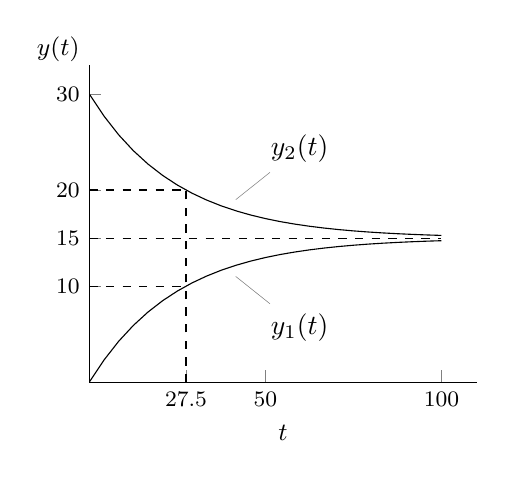
\begin{tikzpicture}
\begin{axis}[small,axis lines*=middle,xmin=0,ymin=0,xlabel={$t$},ylabel={$y(t)$},ylabel style={rotate=-90},ylabel style={at={(axis description cs:0,1.05)}},ytick={0,10,15,20,30},yticklabels={$0$,$10$,$15$,$20$,$30$},xtick={27.465,50,100},xticklabels={$27.5$,$50$,$100$}]
\addplot[domain=0:100]{15-15*e^(-0.04*x)}node[pos=0.4,pin=-45:{$y_1(t)$}]{};
\addplot[domain=0:100]{15+15*e^(-0.04*x)}node[pos=0.4,pin=45:{$y_2(t)$}]{};
\addplot[dashed] plot coordinates {(0,15)(100,15)};
\addplot[dashed] plot coordinates {(27.465,0)(27.465,20)};
\addplot[dashed] plot coordinates {(0,10)(27.465,10)};
\addplot[dashed] plot coordinates {(0,20)(27.465,20)};
\end{axis}
\end{tikzpicture}
\end{subfigure}%
\caption{ٹینکیوں کا نظام۔}
\label{شکل_مثال_نظام_ٹینکیوں_کا_نظام}
\end{figure}

حل:پہلا قدم:\quad نظام کی نمونہ کشی کرتے ہیں۔ ایک ٹینکی کی طرح، ٹینکی الف میں نمک کی مقدار \عددی{y_1(t)} میں تبدیلی کی شرح \عددی{y_1'(t)} نمک کی در آمدی اور بر آمدی شرح میں فرق کے برابر ہو گی۔  یہی کچھ \عددی{y_2'(t)} کے لئے بھی کہا جا سکتا ہے لہٰذا
\begin{align*}
y_1'&=4\frac{y_2}{200}-4\frac{y_1}{200}\\
y_2'&=4\frac{y_1}{200}-4\frac{y_2}{200}
\end{align*}
یعنی
\begin{align*}
y_1'&=-0.02 y_1+0.02y_2\\
y_2'&=\phantom{-}0.02y_1-0.02y_2
\end{align*}
ہو گا۔اس نظام کو
\begin{align}\label{مساوات_نظام_ٹینکی_الف}
\bM{y}'=\bM{A}\bM{y}
\end{align}
لکھا جا سکتا ہے جہاں
\begin{align*}
\bM{y}=
\begin{bmatrix*}[r]
y_1\\
y_2
\end{bmatrix*} \quad \text{اور} \quad 
\bM{A}=
\begin{bmatrix*}[r]
-0.02& \phantom{-}0.02\\
\phantom{-}0.02&-0.02
\end{bmatrix*}
\end{align*}
ہیں۔

دوسرا قدم:\quad عمومی حل حاصل کرتے ہیں۔ ایک عدد تفرقی مساوات کی طرح یہاں بھی حل کو قوت نمائی تفاعل
\begin{align}\label{مساوات_نظام_ٹینکی_ب}
\bM{y}=\bM{x}e^{\lambda t}
\end{align} 
فرض کرتے ہیں۔مساوات \حوالہ{مساوات_نظام_ٹینکی_الف} میں اس فرضی تفاعل اور اس کے تفرق کو پر کرتے ہیں۔
\begin{align*}
 \bM{y}'=\lambda \bM{x}e^{\lambda t}=\bM{A}\bM{x}e^{\lambda t}
\end{align*}
دونوں اطراف کو \عددی{e^{\lambda t}} سے تقسیم کرتے ہوئے دونوں اطراف کو بدل کر لکھتے ہیں۔
\begin{align*}
\bM{A} \bM{x}=\lambda \bM{x}
\end{align*}
ہمیں اس مساوات کے غیر صفر اہم حل درکار ہیں لہٰذا ہمیں \عددی{\bM{A}} کے امتیازی اقدار اور امتیازی سمتیات حاصل کرنے ہوں گے۔امتیازی اقدار امتیازی مساوات
\begin{align*}
\abs{\bM{A}-\lambda \bM{I}}=
\begin{vmatrix*}[r]
-0.02-\lambda& 0.02\\
0.02& -0.02-\lambda
\end{vmatrix*}=
(-0.02-\lambda)-0.02^2=\lambda(\lambda+0.04)=0
\end{align*}
کے حل \عددی{\lambda_1=0} اور \عددی{\lambda_2=-0.04} ہوں گے۔(یہاں دھیان رہے کہ ہمیں غیر صفر امتیازی سمتیات درکار ہیں۔امتیازی اقدار صفر ہو سکتے ہیں۔) امتیازی سمتیات مساوات \حوالہ{مساوات_نظام_امتیازی_ت} کے پہلے یا دوسرے مساوات سے حاصل ہوں گے۔مساوات \حوالہ{مساوات_نظام_امتیازی_ت} کی  پہلے مساوات کو استعمال کرتے ہوئے \عددی{\lambda_1=0} اور \عددی{\lambda_2=-0.04} کے لئے
\begin{align*}
-0.02x_1+0.02x_2=0, \quad (-0.02+0.04)x_1+0.02x_2=0
\end{align*}
لکھے جائیں گے جن سے \عددی{x_1=x_2} اور \عددی{x_1=-x_2} ملتے ہیں۔ہم \عددی{x_1=x_2=1} اور \عددی{x_1=-x_2=1} چنتے ہوئے \عددی{\lambda_1=0} اور \عددی{\lambda_2=-0.04} کے مطابقتی امتیازی سمتیات 
\begin{align*}
\bM{x}^{(1)}=
\begin{bmatrix*}[r]
1\\
1
\end{bmatrix*} \quad \text{اور} \quad
\bM{x}^{(2)}=
\begin{bmatrix*}[r]
1\\
-1
\end{bmatrix*}
\end{align*}
حاصل کرتے ہیں۔مساوات \حوالہ{مساوات_نظام_ٹینکی_ب} اور مسئلہ خطی میل (جو خطی متجانس تفرقی مساوات کے نظام پر بھی لاگو ہوتا ہے) کی مدد سے  حل لکھتے ہیں۔
\begin{align}\label{مساوات_نظام_ٹینکی_پ}
\bM{y}=c_1\bM{x}^{(1)}e^{\lambda_1 t}+c_2\bM{x}^{(2)}e^{\lambda_2 t}=c_1\begin{bmatrix*}[r] 1 \\ 1 \end{bmatrix*}+c_2 \begin{bmatrix*}[r] 1 \\ -1 \end{bmatrix*} e^{-0.04 t}
\end{align}
تیسرا قدم:\quad  ابتدائی معلومات \عددی{y_1(0)=0} (یعنی  ٹینکی الف میں ابتدائی طور پر کوئی نمک نہیں پایا جاتا)  اور \عددی{y_2(0)=30} (یعنی ٹینکی ب میں ابتدائی طور پر تیس کلو گرام نمک پایا جاتا ہے) ہیں۔مساوات \حوالہ{مساوات_نظام_ٹینکی_پ} میں \عددی{t=0} اور ابتدائی معلومات پر کرتے ہیں۔
\begin{align*}
\bM{y}(0)=c_1\begin{bmatrix*}[r] 1 \\ 1 \end{bmatrix*}+c_2 \begin{bmatrix*}[r] 1 \\ -1 \end{bmatrix*}=\begin{bmatrix*}[r] 0 \\ 30 \end{bmatrix*}
\end{align*}
درج بالا مساوات کی جزوی صورت \عددی{c_1+c_2=0} اور \عددی{c_1-c_2=30} ہے جس کا حل \عددی{c_1=15} اور \عددی{c_2=-15} ہے۔یوں ابتدائی معلومات پر پورا اترتا ہوا حل
\begin{align*}
\bM{y}=15\begin{bmatrix*}[r] 1 \\ 1 \end{bmatrix*}-15 \begin{bmatrix*}[r] 1 \\ -1 \end{bmatrix*} e^{-0.04 t}
\end{align*}
یعنی
\begin{align*}
y_1(t)&=15-15e^{-0.04 t}\\
y_2(t)&=15+15e^{-0.04 t}
\end{align*}
ہو گا۔اس حل کو شکل \حوالہ{شکل_مثال_نظام_ٹینکیوں_کا_نظام} میں دکھایا گیا ہے۔

چوتھا قدم: ٹینکی الف میں اس وقت ٹینکی ب کا آدھا نمک ہو گا جب اس میں \عددی{\tfrac{30}{3}=10} کلو گرام نمک ہو۔یوں درج ذیل حاصل ہوتا ہے۔
\begin{align*}
y_1(t)=15-15e^{-0.04 t}=10,\quad t=-\frac{1}{0.04}\ln \frac{1}{3}=\SI{27.5}{\minute}
\end{align*}

\انتہا{مثال}
%===============================
\ابتدا{مثال}\شناخت{مثال_نظام_برقی_جال}\quad برقی جال\\
شکل \حوالہ{شکل_مثال_نظام_برقی_جال} میں لمحہ \عددی{t=0} پر سوئچ چالو ہوتا ہے۔برقی رو \عددی{I_1(t)} اور \عددی{I_2(t)} دریافت کریں۔ابتدائی رو اور ابتدائی برقی گیر میں ذخیرہ بار صفر ہیں۔


\begin{figure}
\centering
\begin{tikzpicture}
\draw(0,0) to [american voltage source,l={${E=\SI{12}{\volt}}$}]++(0,\y) to [cspst,l={${t=0}$}]++(\x,0) to [inductor,l={${L=\SI{1}{\henry}}$}]++(\x,0) to [capacitor,l={${C=\SI{0.4}{\farad}}$}]++(\x,0) to [resistor,l={${R_2=\SI{5}{\ohm}}$}]++(0,-\y) to [short]++(-3*\x,0);
\draw(2*\x,0) to [resistor,*-*,l={${R_1=\SI{6}{\ohm}}$}]++(0,\y);
\draw[stealth-] ([shift={(-150:\x/4)}]3/4*\x,\y/2) arc (-150:150:\x/4);
\draw[stealth-] ([shift={(-150:\x/4)}]2*\x+\x/2,\y/2) arc (-150:150:\x/4);
\draw(3/4*\x,\y/2)node{$I_1$};
\draw(2*\x+\x/2,\y/2)node{$I_2$};
\end{tikzpicture}
\caption{مثال \حوالہ{مثال_نظام_برقی_جال} کا برقی جال۔}
\label{شکل_مثال_نظام_برقی_جال}
\end{figure}

حل:\موٹا{پہلا قدم} نظام کی نمونہ کشی ہے۔امالہ میں رو \عددی{I_1} ہے لہٰذا اس پر برقی دباو \عددی{v_L=L\tfrac{\dif I_1}{\dif t}} ہو گا۔برق گیر میں رو \عددی{I_2} ہے لہٰذا اس پر دباو \عددی{v_C=\tfrac{1}{C}\int I_2 \dif t} ہو گا۔مزاحمت \عددی{R_2} پر دباو \عددی{v_{R2}=I_2R_2} ہو گا جبکہ مزاحمت \عددی{R_1} میں کل رو \عددی{I_1-I_2} ہے لہٰذا اس پر دباو \عددی{v_{R1}=(I_1-I_2)R_1} ہو گا۔کرخوف قانون دباو کے تحت کسی بھی بند دائرے میں کل دباو کا اضافہ اس دائرے میں کل دباو کے گھٹاو کے برابر ہو گا۔یوں بائیں دائرے کے لئے
\begin{align*}
E=L\frac{\dif I_1}{\dif t}+(I_1-I_2)R_1
\end{align*}
لکھا جا سکتا ہے جس میں \عددی{E=12}، \عددی{L=1} اور \عددی{R_1=6} پر کرتے ہوئے
\begin{align}\label{مساوات_مثال_برقی_جال_الف}
I_1'=-6I_1+6I_2+12
\end{align}
ملتا ہے۔اسی طرح دائیں دائرے کے لئے
\begin{align*}
0=\frac{1}{C}\int I_2 \dif t+I_2R_2+(I_2-I_1)R_1
\end{align*}
لکھا جا سکتا ہے جس میں \عددی{C=0.4} اور \عددی{R_2=5} پر کرتے ہوئے تفرق لینے سے
\begin{align*}
I_2+4.4I_2'-2.4I_1'=0
\end{align*}
ملتا ہے۔اس میں مساوات \حوالہ{مساوات_مثال_برقی_جال_الف} سے \عددی{I_1'} کی قیمت پر کرتے ہوئے
\begin{align*}
I_2+4.4I_2'-2.4(-6I_1+6I_2+12)=0
\end{align*}
یعنی
\begin{align}\label{مساوات_مثال_برقی_جال_ب}
I_2'=-\frac{36}{11}I_1+\frac{67}{22}I_2+\frac{72}{11}
\end{align}
حاصل ہوتا ہے۔ مساوات \حوالہ{مساوات_مثال_برقی_جال_الف} اور مساوات \حوالہ{مساوات_مثال_برقی_جال_ب} کو 
\begin{align}\label{مساوات_نظام_برقی_غیر-متجانس_الف}
\bM{J}'=\bM{A} \bM{J}+\bM{g} 
\end{align}
لکھا جا سکتا ہے جہاں 
\begin{align*}
\quad \bM{J}=\begin{bmatrix*}[r] I_1 \\[0.5ex] I_2 \end{bmatrix*},\quad \bM{A}=\begin{bmatrix*}[r] -6 & 6\\[0.5ex] -\frac{36}{11}& \frac{67}{22} \end{bmatrix*}, \quad  \bM{g}=\begin{bmatrix*}[r] 12 \\[0.5ex] \frac{72}{11} \end{bmatrix*}
\end{align*}
ہیں۔\عددی{I_1'} اور \عددی{I_2'} کے  سمتیہ قطار کو \عددی{\bM{J}} اس لئے لکھا گیا ہے کہ اس باب میں \عددی{\bM{I}} اکائی قالب کے لئے استعمال کیا گیا ہے۔ 

\موٹا{دوسرا قدم} نظام کا حل تلاش کرنا ہے۔\عددی{\bM{g}} کی موجودگی  \ترچھا{غیر متجانس سادہ تفرقی نظام} کو ظاہر کرتی ہے لہٰذا ہم ایک عدد تفرقی مساوات کی طرح پہلے متجانس مطابقتی نظام \عددی{\bM{J}'=\bM{A}\bM{J}} کا حل حاصل کرتے ہیں۔ہم \عددی{\bM{J}=\bM{x}e^{\lambda t}} کو حل تصور کرتے ہوئے متجانس نظام میں پر کرتے ہوئے درج ذیل حاصل کرتے ہیں۔
\begin{align*}
\bM{J}'=\lambda \bM{x}e^{\lambda t}=\bM{A}\bM{x}e^{\lambda t} \quad \implies \quad \bM{A}\bM{x}=\lambda \bM{x}
\end{align*}
غیر صفر اہم حل کے حصول کے لئے \عددی{\bM{A}} کے امتیازی اقدار اور امتیازی سمتیات درکار ہوں گے۔امتیازی اقدار امتیازی مساوات
\begin{align*}
\abs{\bM{A}-\lambda \bM{I}}=\begin{vmatrix*}[r] -6-\lambda& 6 \\-\frac{36}{11}&\frac{67}{22}-\lambda \end{vmatrix*}=\lambda^2+\frac{65}{22}\lambda-\frac{15}{11}=0
\end{align*}
سے \عددی{\lambda_1=-2.38209} اور \عددی{\lambda_2=-0.57245} حاصل ہوتے ہیں۔ان امتیازی اقدار کی مطابقتی امتیازی سمتیات مساوات \حوالہ{مساوات_نظام_امتیازی_ت} سے حاصل ہوں گے۔مساوات \حوالہ{مساوات_نظام_امتیازی_ت} کے پہلے مساوات میں  \عددی{\lambda_1} پر کرتے ہوئے 
\begin{align*}
(-6+2.38209)x_1+6x_2&=0,\quad \implies x_1=1.658416x_2
\end{align*}
ملتا ہے۔یوں \عددی{x_2=1} چنتے ہوئے \عددی{x_1=1.658416} ملتا ہے جس سے \عددی{\bM{x}^{(1)}=\begin{bmatrix*} 1.658416 \\1  \end{bmatrix*}} حاصل ہوتا ہے۔اسی طرح مساوات \حوالہ{مساوات_نظام_امتیازی_ت} کے پہلے مساوات میں  \عددی{\lambda_2} پر کرتے ہوئے 
\begin{align*}
(-6+0.57245)x_1+6x_2&=0,\quad \implies x_1=1.105471x_2
\end{align*}
ملتا ہے۔یوں \عددی{x_2=1} چنتے ہوئے \عددی{x_1=1.105471} ملتا ہے جس سے \عددی{\bM{x}^{(2)}=\begin{bmatrix*} 1.105471 \\1  \end{bmatrix*}} حاصل ہوتا ہے۔یوں متجانس نظام کا عمومی حل درج ذیل ہو گا۔
\begin{align}
\bM{J}=c_1\bM{x}^{(1)}e^{\lambda_1 t}+c_2 \bM{x}^{(2)}e^{\lambda_2 t}
\end{align}
مساوات \حوالہ{مساوات_نظام_برقی_غیر-متجانس_الف} کے غیر متجانس نظام کا جبری تفاعل \عددی{\bM{g}} مستقل مقدار ہے لہٰذا اس نظام کا مخصوص حل  مستقل سمتیہ قطار \عددی{\bM{J}_p=\bM{a}} فرض کرتے ہیں جس کے ارکان \عددی{a_1} اور \عددی{a_2} ہیں۔ یوں \عددی{\bM{J}'=0} ہو گا۔ مساوات \حوالہ{مساوات_نظام_برقی_غیر-متجانس_الف} میں فرض کردہ مخصوص حل پر کرتے ہوئے  \عددی{\bM{A}\bM{a}+\bM{g}=0} ملتا ہے جو درج ذیل  مساوات کو ظاہر کرتی ہے۔
\begin{align*}
-6a_1+6a_2+12&=0\\
-\frac{36}{11}a_1+\frac{67}{22}a_2+\frac{72}{11}&=0
\end{align*}
ان ہمزاد مساوات کو حل کرنے سے \عددی{a_1=2} اور \عددی{a_2=0} ملتا ہے لہٰذا \عددی{\bM{a}=\begin{bmatrix*}[r] 2 \\ 0 \end{bmatrix*}} ہو گا۔یوں عمومی حل
\begin{align*}
\bM{J}=\bM{J}_h+\bM{J}_p=c_1\bM{x}^{(1)}e^{\lambda_1 t}+c_2 \bM{x}^{(2)}e^{\lambda_2 t}+\bM{a}
\end{align*}
ہو گا جو درج ذیل مساوات کو ظاہر کرتی ہے۔
\begin{align*}
I_1&=1.658416c_1e^{-2.38209 t}+1.105471c_2e^{-0.57245t}+2\\
I_2&=c_1e^{-2.38209t}+c_2e^{-0.57245t}
\end{align*}
ابتدائی معلومات کے تحت \عددی{I_1(0)=0} اور \عددی{I_2(0)=0} ہے۔انہیں درج بالا مساوات میں پر کرتے  ہوئے
\begin{align*}
1.658416c_1+1.105471c_2+2&=0\\
c_1+c_2&=0
\end{align*}
ملتا ہے جنہیں حل کرتے ہوئے \عددی{c_1=-3.61699} اور \عددی{c_2=3.61699} حاصل ہوتا ہے۔یوں مخصوص حل 
\begin{align*}
\bM{J}=-3.617\bM{x}^{(1)}e^{-2.38t}+3.617\bM{x}^{(2)}e^{-0.57t}+\bM{a}
\end{align*}
یعنی
\begin{align*}
I_1&=-5.998e^{-2.38 t}+3.998e^{-0.57t}+2\\
I_2&=-3.617e^{-2.38t}+3.617e^{-0.57t}
\end{align*}
ہو گا جسے شکل \حوالہ{شکل_مثال_نظام_برقی_جال_مخصوص_حل}-الف میں دکھایا گیا ہے۔
\begin{figure}
\centering
\begin{subfigure}{0.5\textwidth}
\centering
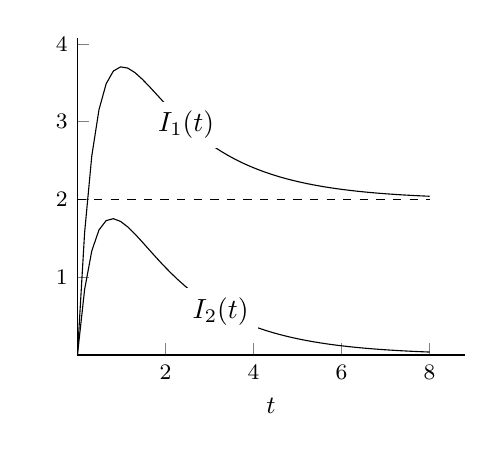
\begin{tikzpicture}
\begin{axis}[small,axis lines*=middle,xlabel={$t$},xmin=0,ymin=0]
\addplot[domain=0:8,samples=50]{-6*e^(-2.38*x)+4*e^(-0.57*x)+2}node[pos=0.5,fill=white]{$I_1(t)$};
\addplot[domain=0:8,samples=50]{-3.617*e^(-2.38*x)+3.617*e^(-0.57*x)}node[pos=0.5,fill=white]{$I_2(t)$};
\addplot[dashed] plot coordinates {(0,2) (8,2)};
\end{axis}
\end{tikzpicture}
\caption*{(الف) مثال \حوالہ{مثال_نظام_برقی_جال} کے دور کا مخصوص حل۔}
\end{subfigure}%
\begin{subfigure}{0.5\textwidth}
\centering
\begin{tikzpicture}
\begin{axis}[small,axis lines*=middle,xlabel={$I_1(t)$},ylabel={$I_2(t)$},xmin=0,xmax=3.9,ymin=0,ylabel style={rotate=-90},ylabel style={at={(axis description cs:0,1.05)}},xlabel style={at={(axis description cs:1.05,0)}}]
\addplot[domain=0:20,samples=150]({-6*e^(-2.38*x)+4*e^(-0.57*x)+2},{-3.617*e^(-2.38*x)+3.617*e^(-0.57*x)})coordinate[pos=0.5](ka)coordinate[pos=0.501](kb);
\draw[-stealth] (ka)--(kb);
\end{axis}
\end{tikzpicture}
\caption*{(ب) \عددی{I_1(t)} بالمقابل \عددی{I_2(t)}}
\end{subfigure}%
\caption{مثال \حوالہ{مثال_نظام_برقی_جال} کے منحنی۔}
\label{شکل_مثال_نظام_برقی_جال_مخصوص_حل}
\end{figure}

شکل \حوالہ{شکل_مثال_نظام_برقی_جال_مخصوص_حل}-ب میں \عددی{I_1(t)} بالمقابل \عددی{I_2(t)} کو \عددی{I_1 I_2} سطح پر دکھایا گیا ہے جس میں \عددی{t} مقدار معلوم  ہے۔مقدار معلوم کے بڑھنے کی سمت کو منحنی پر تیر کے نشان سے دکھایا گیا ہے۔ سطح \عددی{I_1 I_2} کو نظام کی \اصطلاح{سطح مرحلہ}\فرہنگ{سطح مرحلہ}\حاشیہب{phase plane}\فرہنگ{phase plane} کہتے ہیں جبکہ شکل \حوالہ{شکل_مثال_نظام_برقی_جال_مخصوص_حل}-ب کی منحنی کو \اصطلاح{خط حرکت}\فرہنگ{خط حرکت}\حاشیہب{trajectory}\فرہنگ{trajectory} کہتے ہیں۔ہم دیکھیں گے کہ \ترچھا{سطح مرحلہ اشکال}،  سادہ شکل \حوالہ{شکل_مثال_نظام_برقی_جال_مخصوص_حل}-الف طرز کے اشکال سے زیادہ اہم ثابت ہوتے ہیں۔یہ خطوط کی نسل کے بارے میں بہتر کیفی  معلومات فراہم کرتے ہیں۔
\انتہا{مثال}
%=============================

صفحہ \حوالہصفحہ{مثال_سادہ_اول_مرکب} مثال \حوالہ{مثال_سادہ_اول_مرکب} میں ایک عدد ٹینکی کی مثال پر غور کیا گیا جس کی نمونہ کشی ایک عدد سادہ تفرقی مساوات سے کی گئی۔ مثال \حوالہ{مثال_نظام_ٹینکیوں_کا_نظام} میں دو ٹینکیوں پر مبنی نظام کی نمونہ کشی  دو عدد تفرقی مساوات سے کی گئی۔ اسی طرح مثال \حوالہ{مثال_نظام_برقی_جال} میں دو عدد نا معلوم رو کی بنا دو عدد سادہ تفرقی مساوات حاصل ہوئے۔آپ دیکھ سکتے ہیں کہ زیادہ بڑے نظام کی نمونہ کشی زیادہ تعداد کی تفرقی مساوات سے کی جائے گی۔
%=======================

\جزوحصہء{\عددی{n} رتبی سادہ تفرقی مساوات سے تفرقی مساوات کے نظام کا حصول}
درج ذیل مسئلہ میں ثابت کیا جاتا ہے کہ \عددی{n} رتبی سادہ تفرقی مساوات \حوالہ{مساوات_بلند_درجی_سے_سادہ_الف} سے تفرقی مساوات کا نظام حاصل کیا جا سکتا ہے۔

\ابتدا{مسئلہ}\quad تفرقی مساوات کا مبادلہ\\
سادہ \عددی{n} رتبی تفرقی مساوات
\begin{align}\label{مساوات_بلند_درجی_سے_سادہ_الف}
y^{(n)}=F(t,y,y',\cdots,y^{(n-1)})
\end{align}
میں
\begin{align}\label{مساوات_بلند_درجی_سے_سادہ_ب}
y_1=y,\quad y_2=y',\quad y_3=y'', \cdots, y_n=y^{(n-1)}
\end{align}
لے کر اس کو  \عددی{n} عدد سادہ یک رتبی تفرقی مساوات کے نظام
\begin{gather}
\begin{aligned}\label{مساوات_بلند_درجی_سے_سادہ_پ}
y_1'&=y_2\\
y_2'&=y_3\\
\vdots\\
y_{n-1}'&=y_n\\
y_n'&=F(t,y_1,y_2,\cdots,y_n)
\end{aligned}
\end{gather}
 میں تبدیل کیا جا سکتا ہے۔
\انتہا{مسئلہ}
%==========================
\ابتدا{ثبوت}
مساوات \حوالہ{مساوات_بلند_درجی_سے_سادہ_ب} کے تفرق سے نظام کے پہلے \عددی{n-1} عدد تفرقی مساوات حاصل ہوتے ہیں۔مساوات \حوالہ{مساوات_بلند_درجی_سے_سادہ_ب} سے \عددی{y_n'=y^{(n)}} بھی حاصل ہوتا ہے لہٰذا مساوات \حوالہ{مساوات_بلند_درجی_سے_سادہ_الف} سے مساوات \حوالہ{مساوات_بلند_درجی_سے_سادہ_پ} کی آخری مساوات بھی حاصل ہوتی ہے۔
\انتہا{ثبوت}
%============================

\ابتدا{مثال}\شناخت{مثال_نظام_اسپرنگ_کمیت}
ہم  اسپرنگ اور کمیت کی آزادانہ ارتعاش  کے مسئلے پر غور کر چکے ہیں جس کی تفرقی مساوات صفحہ \حوالہصفحہ{مساوات_سادہ_دو_درجی_قصری_نظام_الف} پر مساوات \حوالہ{مساوات_سادہ_دو_درجی_قصری_نظام_الف}
\begin{align}
my''+cy'+ky=0 \quad \implies \quad y''=-\frac{k}{m}y-\frac{c}{m}y'
\end{align}
 دیتی ہے جس کے لئے مساوات \حوالہ{مساوات_بلند_درجی_سے_سادہ_پ} کا نظام
\begin{align*}
y_1'&=y_2\\
y_2'&=-\frac{k}{m}y_1-\frac{c}{m}y_2
\end{align*}
 متجانس اور خطی ہے۔قالب کا استعمال کرتے ہوئے \عددی{\bM{y}=\begin{bmatrix*}[r] y_1 \\ y_2 \end{bmatrix*}} لکھتے ہوئے اس نظام کو درج ذیل لکھا جا سکتا ہے
\begin{align}
\bM{y}'=\bM{A}\bM{y}=\begin{bmatrix*}[r] 0 & 1 \\ -\frac{k}{m}& -\frac{c}{m} \end{bmatrix*}\begin{bmatrix*}[r]  y_1 \\ y_2 \end{bmatrix*}
\end{align}
جس سے امتیازی مساوات لکھتے ہیں۔
\begin{align*}
\abs{\bM{A}-\lambda \bM{I}}=\begin{vmatrix*}[r] -\lambda & 1\\ -\frac{k}{m}& -\frac{c}{m}-\lambda \end{vmatrix*}=\lambda^2+\frac{c}{m}\lambda+\frac{k}{m}=0
\end{align*}
اب مثلاً \عددی{m=1}، \عددی{c=1.4} اور \عددی{k=0.24} ہوں تب 
\begin{align*}
\lambda^2+1.4\lambda+0.24=(\lambda+0.2)(\lambda+1.2)=0
\end{align*}
ہو گا جس سے امتیازی اقدار \عددی{\lambda_1=-0.2} اور \عددی{\lambda_2=-1.2} حاصل ہوتے ہیں۔امتیازی سمتیات \عددی{\bM{A}-\lambda \bM{I}=\bM{0}} کی پہلی مساوات \عددی{-\lambda x_1+x_2} سے حاصل کرتے ہیں۔امتیازی قدر \عددی{\lambda_1=-0.2} پر کرتے ہوئے  \عددی{0.2x_1+x_2=0} سے \عددی{x_2=-0.2x_1} ملتا ہے لہٰذا \عددی{x_1=1} چنتے ہوئے \عددی{x_2=-0.2} ہو گا۔اسی طرح \عددی{\lambda_2=-1.2} پر کرتے ہوئے \عددی{1.2x_1+x_2=0} سے \عددی{x_2=-1.2x_1} ملتا ہے لہٰذا \عددی{x_1=1} چنتے ہوئے \عددی{x_2=-1.2} ہو گا۔یوں درج ذیل امتیازی سمتیات حاصل ہوتی ہیں
\begin{align*}
\bM{x}^{(1)}=\begin{bmatrix*} 1 \\ -0.2  \end{bmatrix*}, \quad \bM{x}^{(2)}=\begin{bmatrix*}  1 \\ -1.2 \end{bmatrix*}
\end{align*}
جنہیں استعمال کرتے ہوئے
\begin{align*}
\bM{y}=c_1\begin{bmatrix*} 1 \\ -0.2  \end{bmatrix*}e^{-0.2 t}+c_2 \begin{bmatrix*}  1 \\ -1.2 \end{bmatrix*} e^{-1.2 t}
\end{align*}
سمتیہ حل لکھا جائے گا۔اس نظام کی پہلی مساوات
\begin{align*}
y=y_1=c_1e^{-0.2 t}+c_2e^{-1.2 t}
\end{align*}
درکار حل ہے جبکہ نظام کی دوسری مساوات حل کی تفرق ہے۔
\begin{align*}
y_2=y_1'=y'=-0.2c_1e^{-0.2 t}-1.2c_2e^{-1.2t}
\end{align*}
\انتہا{مثال}
%=================================

\حصہء{سوالات}
سوال \حوالہ{سوال_نظام_امتیازی_الف} تا سوال \حوالہ{سوال_نظام_امتیازی_ب} میں دیے گئے قالب کے امتیازی اقدار اور امتیازی سمتیات حاصل کریں۔

%===================
\ابتدا{سوال}\شناخت{سوال_نظام_امتیازی_الف}
الیکٹران کی ایک خاصیت  \اصطلاح{چکر}\فرہنگ{چکر}\حاشیہب{spin}\فرہنگ{spin} کہلاتی ہے جس کی مقدار  \عددی{-\tfrac{\hbar}{2}} یا \عددی{\tfrac{\hbar}{2}} ہو سکتی ہے  جہاں \عددی{\hbar=\tfrac{h}{2\pi}} ہے اور \عددی{h=\SI{6.626e-34}{\meter^2\kilo\gram\per\second}} \اصطلاح{مستقل پلانک}\فرہنگ{مستقل پلانک}\حاشیہب{Plank's constant}\فرہنگ{Plank' constant}  ہے۔\اصطلاح{چکر} سمتیہ مقدار ہے۔مقناطیسی میدان میں الیکٹران کا \اصطلاح{چکر}  یا ہمہ میدان (مقناطیسی میدان کی سمت میں) رہتا ہے اور یا مخالف میدان (میدان کی الٹ سمت میں) رہتا ہے۔ہمہ میدان صورت میں الیکٹران کو \اصطلاح{اوپر چکر}\فرہنگ{اوپر چکر}\فرہنگ{اوپر چکر}\حاشیہب{spin up}\فرہنگ{spin up} الیکٹران کہتے ہیں جبکہ میدان مخالف چکر کی صورت میں  الیکٹران کو \اصطلاح{نیچے چکر}\فرہنگ{نیچے چکر}\حاشیہب{spin down}\فرہنگ{spin down} الیکٹران کہتے ہیں۔\عددی{z} سمت میں مقناطیسی میدان میں موجود الیکٹران کی خاصیت \عددی{\bM{S}_z} \اصطلاح{قالب چکر}\فرہنگ{قالب چکر}\حاشیہب{spin matrix}\فرہنگ{spin matrix} سے معلوم کی جا سکتی ہے۔\عددی{z} میدان میں \ترچھا{اوپر چکر} الیکٹران کو امتیازی سمتیہ \عددی{\chi^z_+} اور \ترچھا{نیچے چکر} الیکٹران کو امتیازی سمتیہ \عددی{\chi^z_-} سے ظاہر کیا جاتا ہے۔ درج ذیل \عددی{\bM{S}_z} قالب کے امتیازی اقدار (یعنی الیکٹران کا چکر) حاصل کرتے ہوئے امتیازی سمتیات دریافت کریں۔
 \begin{align*}
\bM{S}_z=\begin{bmatrix*}[r] \frac{\hbar}{2} & 0\\ 0 & -\frac{\hbar}{2}\end{bmatrix*}
\end{align*}
جوابات:\عددی{\lambda_-=-\tfrac{\hbar}{2}}، \عددی{\lambda_+=\tfrac{\hbar}{2}}، \عددی{\chi^z_-=\begin{bmatrix*}[r] 0 \\ 1 \end{bmatrix*}}،  \عددی{\chi^z_+=\begin{bmatrix*}[r] 1 \\ 0 \end{bmatrix*}}
\انتہا{سوال}
%==================
\ابتدا{سوال}
مقناطیسی میدان میں الیکٹران کی زاویائی حرکت کے معیار اثر کا مربع \عددی{\bM{S}^2} قالب سے ظاہر کیا جاتا ہے۔اس قالب کی امتیازی قدر زاویائی حرکت کے معیار اثر کا مربع ہو گا۔قالب کی امتیازی قدر اور امتیازی سمتیات دریافت کریں۔
  \begin{align*}
\bM{S}^2=\begin{bmatrix*}\frac{3\hbar}{4} & 0\\ 0 & \frac{3\hbar}{4}\end{bmatrix*}
\end{align*}
جوابات:\عددی{\lambda_1=\lambda_2=\tfrac{3\hbar^2}{4}}،  \عددی{\begin{bmatrix*}[r] 0 \\ 1 \end{bmatrix*}}، 
 \عددی{\begin{bmatrix*}[r] 1 \\ 0 \end{bmatrix*}}
\انتہا{سوال}
%===================
\ابتدا{سوال}\quad 
$\bM{A}=\begin{bmatrix*}[r] 1& -1\\ 0&1 \end{bmatrix*}$\\
جوابات:\عددی{\lambda_1=\lambda_2=1}، \عددی{\bM{x}^{(1)}=\bM{x}^{(2)}=\begin{bmatrix*}[r] 1 \\0 \end{bmatrix*}}
\انتہا{سوال}
%=====================
\ابتدا{سوال}\quad
$\bM{A}=\begin{bmatrix*}[r] 1& -1\\ 1&0 \end{bmatrix*}$\\
جوابات:\عددی{\lambda_1=\tfrac{1}{2}-\tfrac{\sqrt{3}}{2}i}،  \عددی{\lambda_2=\tfrac{1}{2}+\tfrac{\sqrt{3}}{2}i}، 
\عددی{\bM{x}^{(1)}=\begin{bmatrix*} 1 \\ \tfrac{1}{2}+\tfrac{\sqrt{3}}{2}i \end{bmatrix*}}، \عددی{\bM{x}^{(2)}=\begin{bmatrix*} 1 \\ \tfrac{1}{2}-\tfrac{\sqrt{3}}{2}i \end{bmatrix*}}
\انتہا{سوال}
%=====================
\ابتدا{سوال}\شناخت{سوال_نظام_امتیازی_ب}\
$\bM{A}=\begin{bmatrix*}[r] 0.2& 0.6\\ -0.4&1.2 \end{bmatrix*}$\\
جوابات:\عددی{\lambda_1=\tfrac{3}{5}}،  \عددی{\lambda_2=\tfrac{4}{5}}، 
\عددی{\bM{x}^{(1)}=\begin{bmatrix*}[r] 1 \\ \tfrac{2}{3} \end{bmatrix*}}،
 \عددی{\bM{x}^{(2)}=\begin{bmatrix*}[r] 1 \\ 1\end{bmatrix*}}
\انتہا{سوال}
%=====================

سوال \حوالہ{سوال_نظام_ٹینکی_الف} اور سوال \حوالہ{سوال_نظام_ٹینکی_ب} ٹینکیوں کے سوالات ہیں۔

%==============
\ابتدا{سوال}\شناخت{سوال_نظام_ٹینکی_الف}
اگر مثال \حوالہ{مثال_نظام_ٹینکیوں_کا_نظام} میں ٹینکی الف میں ابتدائی طور پر چار سو \عددی{(400)} لٹر پانی موجود ہو تب جوابات کیا ہوں گے؟

جوابات:\عددی{\bM{A}=\begin{bmatrix*}[r] -0.01 & 0.02 \\ 0.01 & -0.02 \end{bmatrix*}}، \عددی{\lambda_1=-0.03}، 
\عددی{\lambda_2=0}، \عددی{\bM{x}^{(1)}=\begin{bmatrix*}[r] 1 \\ -1  \end{bmatrix*}}، \\
\عددی{\bM{x}^{(2)}=\begin{bmatrix*}[r] 1 \\0.5  \end{bmatrix*}}،\عددی{c_1=-20}، \عددی{c_2=20}، \عددی{\SI{23.1}{\minute}} 
\انتہا{سوال}
%======================
\ابتدا{سوال}\شناخت{سوال_نظام_ٹینکی_ب}
مثال \حوالہ{مثال_نظام_ٹینکیوں_کا_نظام} میں  ٹینکی الف کے ساتھ دو سو \عددی{(200)} لٹر کی ٹینکی پ دو نالیوں کے ذریعہ جوڑی جاتی ہے۔ان کے مابین بھی چار لٹر فی منٹ کی شرح سے پانی کا تبادلہ ہوتا ہے۔ٹینکی پ میں ابتدائی طور پر دو سو لٹر کا خالص پانی پایا جاتا ہے۔اس نظام کے تفرقی مساوات لکھ کر \عددی{\bM{A}} حاصل کریں۔نظام کے امتیازی اقدار اور امتیازی سمتیات دریافت کرتے ہوئے مخصوص حل دریافت کریں۔

جوابات:\عددی{\bM{A}=\begin{bmatrix*} -0.04 & 0.02 & 0.02 \\ 0.02 &-0.02 & 0\\ 0.02 & 0 &-0.02 \end{bmatrix*}}، \عددی{\lambda_1=-0.06}، \عددی{\lambda_2=-0.02}، \عددی{\lambda_3=0}، \عددی{\bM{x}^{(1)}=\begin{bmatrix*} 1 \\ -0.5 \\ -0.5  \end{bmatrix*}}،
 \عددی{\bM{x}^{(2)}=\begin{bmatrix*}[r] 0 \\ 1 \\ -1  \end{bmatrix*}}، \عددی{\bM{x}^{(3)}=\begin{bmatrix*}[r] 1 \\ 1 \\ 1  \end{bmatrix*}}،\\
 \عددی{\bM{y}=-10\bM{x}^{(1)}e^{-0.06t}+15\bM{x}^{(-0.02t)}+10\bM{x}^{(3)}}
\انتہا{سوال}
%====================

سوال \حوالہ{سوال_نظام_جال_الف} تا سوال \حوالہ{سوال_نظام_جال_ب} برقی جال پر مبنی ہیں۔

%================
\ابتدا{سوال}\شناخت{سوال_نظام_جال_الف}
اگر مثال \حوالہ{مثال_نظام_برقی_جال} میں ابتدائی برقی رو \عددی{I_1(0)=0} اور \عددی{I_2=\SI{2}{\ampere}} ہوں تب حل کیا ہو گا؟

جواب:\عددی{I_1=10.63e^{-0.57t}-12.63e^{-2.38t}+2}، \عددی{I_2=9.62e^{-0.57t}-7.62e^{-2.38t}}
\انتہا{سوال}
%===================
\ابتدا{سوال}
اگر مثال \حوالہ{مثال_نظام_برقی_جال} میں  \عددی{L=\SI{0.5}{\henry}} کر دیا جائے  تب مخصوص حل کیا ہو گا؟

جواب:\عددی{I_1=2.96e^{-0.529t}-4.96e^{-5.153t}+2}، \عددی{I_2=2.83e^{-0.529t}-2.83e^{-5.153t}}
\انتہا{سوال}
%===================
\ابتدا{سوال}\شناخت{سوال_نظام_جال_ب}
اگر مثال \حوالہ{مثال_نظام_برقی_جال} میں  \عددی{L=\SI{2}{\henry}} کر دیا جائے  تب مخصوص حل کیا ہو گا؟

جواب:\عددی{I_1=2+e^{-\tfrac{35}{44}t}[19.9\cos (0.22t)-2\sin(0.22t)]}، \عددی{I_2=14.77e^{-\tfrac{35}{44}t}\sin(0.22t)}
\انتہا{سوال}
%===================

سوال \حوالہ{سوال_نظام_تبدیلی_الف} تا سوال \حوالہ{سوال_نظام_تبدیلی_الف} میں تفرقی مساوات کو نظام میں تبدیل کرتے ہوئے \عددی{\bM{A}} قالب حاصل کریں۔اس قالب کے امتیازی اقدار اور امتیازی سمتیات دریافت کریں۔مساوات کا عمومی حل حاصل کریں۔ تفرقی مساوات کو جوں کا توں بھی حل کریں۔

%===================
\ابتدا{سوال}\شناخت{سوال_نظام_تبدیلی_الف}\quad 
$y''+5y'+6y=0$\\
جوابات:\عددی{\bM{A}=\begin{bmatrix*}[r] 0 & 1 \\ -6 & -5  \end{bmatrix*}}، \عددی{\lambda_1=-3}، \عددی{\lambda_2=-2}،
 \عددی{\bM{x}^{(1)}=\begin{bmatrix*}[r]  1 \\ -3  \end{bmatrix*}}،  \عددی{\bM{x}^{(2)}=\begin{bmatrix*}[r]  1 \\ -2  \end{bmatrix*}}،
$\bM{y}=c_1\begin{bmatrix*}[r] 1 \\ -3 \end{bmatrix*} e^{-3t}+c_2\begin{bmatrix*}[r] 1 \\ -2 \end{bmatrix*} e^{-2t}$ 
\انتہا{سوال}
%===================
\ابتدا{سوال}\quad 
$12y''-y'-6y=0$\\
جوابات:\عددی{\bM{A}=\begin{bmatrix*}[r] 0 & 1 \\ \tfrac{1}{2} & \tfrac{1}{12}  \end{bmatrix*}}، \عددی{\lambda_1=-\tfrac{2}{3}}، 
\عددی{\lambda_2=\tfrac{3}{4}}، \عددی{\bM{x}^{(1)}=\begin{bmatrix*}[r]  1 \\ -\tfrac{2}{3}  \end{bmatrix*}}، 
 \عددی{\bM{x}^{(2)}=\begin{bmatrix*}[r]  1 \\ \tfrac{3}{4}  \end{bmatrix*}}،
$\bM{y}=c_1\begin{bmatrix*}[r] 1 \\ -\tfrac{2}{3} \end{bmatrix*} e^{-\tfrac{2}{3}t}+c_2\begin{bmatrix*}[r] 1 \\ \tfrac{3}{4} \end{bmatrix*} e^{\tfrac{3}{4}t}$ 
\انتہا{سوال}
%===================
\ابتدا{سوال}\quad 
$y'''-y'=0$\\
جوابات:\عددی{\bM{A}=\begin{bmatrix*}[r] 0 & 1 &0\\0 & 0&1 \\ 0&1&0  \end{bmatrix*}}،
 \عددی{\lambda_1=-1}، 
\عددی{\lambda_2=1}، \عددی{\lambda_3=0}، \عددی{\bM{x}^{(1)}=\begin{bmatrix*}[r]  1 \\ -1 \\ 1  \end{bmatrix*}}، 
 \عددی{\bM{x}^{(2)}=\begin{bmatrix*}[r]  1 \\ 1 \\ 1  \end{bmatrix*}}،  \عددی{\bM{x}^{(3)}=\begin{bmatrix*}[r]  1 \\ 0 \\ 0  \end{bmatrix*}}، 
$\bM{y}=c_1\begin{bmatrix*}[r] 1 \\ -1 \\ 1 \end{bmatrix*} e^{-t}+c_2\begin{bmatrix*}[r] 1 \\ 1 \\ 1 \end{bmatrix*} e^{t}+c_3 \begin{bmatrix*}[r] 1 \\ 0 \\ 0 \end{bmatrix*}$ 
\انتہا{سوال}
%===================
\ابتدا{سوال}\quad 
$y''+9y'+14y=0$\\
جوابات:\عددی{\bM{A}=\begin{bmatrix*}[r] 0 & 1 \\-14 & -9  \end{bmatrix*}}،
 \عددی{\lambda_1=-2}، \عددی{\lambda_2=-7}، \عددی{\bM{x}^{(1)}=\begin{bmatrix*}[r]  1 \\ -2  \end{bmatrix*}}، \\
 \عددی{\bM{x}^{(2)}=\begin{bmatrix*}[r]  1 \\ -7  \end{bmatrix*}}، 
$\bM{y}=c_1\begin{bmatrix*}[r] 1 \\ -2 \end{bmatrix*} e^{-2t}+c_2\begin{bmatrix*}[r] 1 \\ -7 \end{bmatrix*} e^{-7t}$ 
\انتہا{سوال}
%===================
\ابتدا{سوال}
دو اسپرنگ اور دو کمیت کا نظام شکل \حوالہ{شکل_نظام_اسپرنگ_کمیت_نظام} میں دکھایا گیا ہے جس میں \عددی{m_1=m_2=1}، \عددی{k_1=3} اور \عددی{k_2=4} ہیں۔اس نظام  کے تفرقی مساوات  لکھیں۔\عددی{\bM{y}=\bM{x}e^{\omega t}} تصور کرتے ہوئے، جہاں \عددی{\omega^2=\lambda} ہے، ان کا حل دریافت کریں۔
 
\begin{figure}
\centering
\begin{tikzpicture}
\node[circle,fill=gray,inner sep=2.5mm] (a) at (0,-0.5) {};
\node[circle,fill=gray,inner sep=2.5mm] (aa) at (0,-3) {};
\node[circle,fill=gray,inner sep=2.5mm] (b) at (3,0) {};
\node[circle,fill=gray,inner sep=2.5mm] (bb) at (3,-2) {};
\draw[decoration={aspect=0.3, segment length=2.3mm, amplitude=3mm,coil},decorate] (0,2) -- (a); 
\draw[decoration={aspect=0.3, segment length=2.5mm, amplitude=3mm,coil},decorate] (0,-0.5-0.4) -- (aa)
node[pos=0.5,shift={(-0.75,0)},left]{\RL{اضافہ $(y_2-y_1)$ ہے}}++(0,-0.75)node[]{\RL{ارتعاش پذیر نظام}}; 
\draw(0,-0.5-0.4)--++(0,0.05);
\draw[decoration={aspect=0.3, segment length=1.7mm, amplitude=3mm,coil},decorate] (3,2) -- (b)node[pos=0.5,shift={(0.75,0)}]{$k_1$}; 
\draw[decoration={aspect=0.3, segment length=1.7mm, amplitude=3mm,coil},decorate] (3,-0.4) -- (bb)node[pos=0.5,shift={(0.75,0)}]{$k_2$}++(0,-0.75)node[]{\RL{ساکن نظام}}; 
\draw(3,-0.4)--++(0,0.05);
\fill [pattern = north east lines] (-1,2) rectangle ++(5,0.2);
\draw[thick] (-1,2) -- ++(5,0);
%dashed lines
\draw[dashed](b)--++(-2,0)coordinate[pos=0.8](bL);
\draw[dashed](b)--++(1,0)node[right]{$(y_1=0)$};
\draw[dashed](bb)--++(-2,0)coordinate[pos=0.8](bbL);
\draw[dashed](bb)--++(1,0)node[right]{$(y_2=0)$};
\draw[dashed](a)--++(1.5,0)coordinate(aR);
\draw[dashed](aa)--++(1.5,0)coordinate(aaR);
%dimensions
\draw[-stealth] (bL)--($(a)!(bL)!(aR)$)node[pos=0.5,right]{$y_1$};
\draw[-stealth] (bbL)--($(aa)!(bbL)!(aaR)$)node[pos=0.5,right]{$y_2$};
\end{tikzpicture}
\caption{دو اسپرنگ اور دو کمیت کا نظام۔}
\label{شکل_نظام_اسپرنگ_کمیت_نظام}
\end{figure}

جوابات:\عددی{y_1=A\cos (1.109t)+B\sin (1.109t)+C\cos (3.126t)+D\sin (3.126t)}، \\
\عددی{\عددی{y_2=A^*\cos (1.109t)+B^*\sin (1.109t)+C^*\cos (3.126t)+D^*\sin (3.126t)}}
\انتہا{سوال}
%=======================

\حصہ{نظریہ نظام سادہ تفرقی مساوات اور ورونسکی}\شناخت{حصہ_نظام_نظریہ_نظام}
گزشتہ حصے کے یک رتبی تفرقی مساوات کے نظام، درج ذیل عمومی نظام کی مخصوص صورت ہے۔
\begin{gather}
\begin{aligned}\label{مساوات_نظام_عمومی_الف}
y_1&=f_1(t,y_1,\cdots,y_n)\\
y_2&=f_2(t,y_1,\cdots,y_n)\\
\vdots &\\
y_n&=f_n(t,y_1,\cdots,y_n)
\end{aligned}\quad \implies \quad
\begin{aligned}
\bM{y}'=\bM{f}(t,\bM{y})
\end{aligned}
\end{gather}
نظام کو سمتیہ کی صورت میں سمتیہ قطار \عددی{\bM{y}=[y_1,y_2,\cdots,y_n]^T} اور سمتیہ قطار \عددی{\bM{f}=[f_1,f_2,\cdots,f_n]^T} (یہاں $T$ سے مراد تبدیلی محل ہے جسے استعمال کرتے ہوئے سمتیہ قطار کو افقی لکھ کر جگہ بچائی گئی ہے) کی استعمال سے لکھا گیا ہے۔درج بالا نظام عملی استعمال کے تقریباً تمام صورتوں کو ظاہر کرتی ہے۔یوں \عددی{n=1} کی صورت میں یہ \عددی{y_1'=f_1(t,y_1)} یعنی \عددی{y'=f(t,y)} کو ظاہر کرے گی جسے ہم باب \حوالہ{باب_سادہ_اول_تفرقی} سے جانتے ہیں۔ 

کسی کھلے وقفہ \عددی{a < t <b} پر مساوات \حوالہ{مساوات_نظام_عمومی_الف} کا \موٹا{حل}، وقفہ \عددی{a < t <b} پر قابل تفرق، \عددی{n} عدد  تفاعل کا سلسلہ
\begin{align*}
y_1=h_1(t),\quad y_2=h_2(t),\quad \cdots, \quad y_n=h_n(t)
\end{align*}
ہو گا جو  پورے  وقفے پر مساوات \حوالہ{مساوات_نظام_عمومی_الف} پر پورا اترتا ہو۔\اصطلاح{حل سمتیہ}\فرہنگ{حل سمتیہ}\حاشیہب{solution vector}\فرہنگ{solution vector} کو قطار سمتیہ \عددی{\bM{h}=[h_1(t),\cdots,h_n(t)]^T} کی صورت میں لکھا جا سکتا ہے۔
\begin{align*}
\bM{y}=\bM{h}(t)
\end{align*}
اس نظام پر مبنی \اصطلاح{ابتدائی قیمت مسئلہ} مساوات \حوالہ{مساوات_نظام_عمومی_الف} اور  \عددی{n} عدد \اصطلاح{ابتدائی شرائط} 
\begin{align}\label{مساوات_نظام_عمومی_ب}
y_1(t_0)=K_1, \quad y_2(t_0)=K_2,\quad \cdots,\quad y_n(t_0)=K_n
\end{align}
پر مبنی ہو گا۔ان ابتدائی شرائط کو سمتیہ کی صورت میں \عددی{\bM{y}(t_0)=\bM{K}} لکھا جا سکتا ہے جہاں \عددی{t_0} دیے گئے وقفے پر پایا جاتا ہے اور سمتیہ قطار \عددی{\bM{K}=[K_1,\cdots,K_n]^T} کے ارکان دیے گئے مستقل مقدار ہیں۔مساوات \حوالہ{مساوات_نظام_عمومی_الف} اور مساوات \حوالہ{مساوات_نظام_عمومی_ب} کے ابتدائی قیمت مسئلے کے حل کی \ترچھا{وجودیت} اور \ترچھا{یکتائی} کے لئے \ترچھا{کافی شرائط} درج ذیل مسئلہ بیان کرتی ہے جو حصہ \حوالہ{حصہ_اول_وجودیت_یکتائی} میں دیے گئے مسئلے کو وسعت دیتی ہے۔اس مسئلے کا ثبوت اس کتاب میں پیش نہیں کیا جائے گا۔
%===============

\ابتدا{مسئلہ}\شناخت{مسئلہ_نظام_وجودیت_یکتائی_نظام}\quad مسئلہ وجودیت اور یکتائی \\
تصور کریں کہ فضا \عددی{ty_1y_2\cdots y_n} کے \اصطلاح{دائرہ کار}\فرہنگ{دائرہ کار}\حاشیہب{domain}\فرہنگ{domain} \عددی{R} میں  تفاعل \عددی{f_1} تا \عددی{f_n} اور ان کے تفرق \عددی{\tfrac{\partial f_1}{\partial y_1}}، \نقطے  \عددی{\tfrac{\partial f_1}{\partial y_n}}،\نقطے  \عددی{\tfrac{\partial f_n}{\partial y_n}} استمراری ہوں اور اس دائرہ کار میں نقطہ \عددی{(t_0,K_1,\cdots,K_n)} پایا جاتا ہو تب کسی وقفہ \عددی{t_0-\alpha<t<t_0+\alpha} پر مساوات \حوالہ{مساوات_نظام_عمومی_الف} کا ایسا حل \ترچھا{موجود} ہو گا جو مساوات \حوالہ{مساوات_نظام_عمومی_ب} کی ابتدائی شرائط پر پورا اترتا ہو اور  یہ حل \ترچھا{یکتا} ہو گا۔
\انتہا{مسئلہ}
%===================

\جزوحصہ{خطی نظام}
سادہ تفرقی مساوات کے \ترچھا{خطی} ہونے کی تصور کو وسعت دیتے ہوئے ہم مساوات \حوالہ{مساوات_نظام_عمومی_الف} کو اس صورت \اصطلاح{خطی نظام}\فرہنگ{خطی نظام}\حاشیہب{linear system}\فرہنگ{linear system} کہیں گے جب اس کو
\begin{gather}
\begin{aligned}\label{مساوات_خطی_نظام_الف}
y_1'&=a_{11}(t)y_1+\cdots+a_{1n}(t)y_n+g_1(t)\\
y_2'&=a_{21}(t)y_1+\cdots+a_{2n}(t)y_n+g_2(t)\\
\vdots\\
y_n'&=a_{n1}(t)y_1+\cdots+a_{nn}(t)y_n+g_n(t)
\end{aligned}\quad \implies \quad
\bM{y}'=\bM{A}\bM{y}+\bM{g}
\end{gather}
لکھنا ممکن ہو جہاں
\begin{align*}
\bM{A}=
\begin{bmatrix}
a_{11} & a_{12}&\cdots & a_{1n}\\
a_{21} & a_{22}&\cdots & a_{2n}\\
&\vdots & &\\
a_{n1} & a_{n2}&\cdots & a_{nn}
\end{bmatrix}, \quad 
\bM{y}=
\begin{bmatrix}
y_1\\
y_2\\
\vdots\\
y_n
\end{bmatrix}, \quad 
\bM{g}=
\begin{bmatrix}
g_1\\
g_2\\
\vdots\\
g_n
\end{bmatrix}
\end{align*}
ہیں۔آپ دیکھ سکتے ہیں کہ نظام \حوالہ{مساوات_خطی_نظام_الف} میں \عددی{y_1'} تا \عددی{y_n'} کا \عددی{y_1} تا \عددی{y_n} کے ساتھ \ترچھا{خطی} تعلق ہے۔ اگر \عددی{\bM{g}=0} ہو تب نظام \حوالہ{مساوات_خطی_نظام_الف}
\begin{align}\label{مساوات_خطی_نظام_ب}
\bM{y}'=\bM{A}\bM{y}
\end{align}
صورت اختیار کرتا ہے جو  \اصطلاح{متجانس} نظام ہے جبکہ \عددی{\bM{g} \ne 0} کی صورت میں نظام \حوالہ{مساوات_خطی_نظام_الف} کو \اصطلاح{غیر متجانس} کہلاتا ہے۔یوں مثال \حوالہ{مثال_نظام_ٹینکیوں_کا_نظام} اور مثال \حوالہ{مثال_نظام_اسپرنگ_کمیت} متجانس نظام ہیں جبکہ مثال \حوالہ{مثال_نظام_برقی_جال} غیر متجانس نظام ہے۔

خطی نظام میں \عددی{\tfrac{\partial f_1}{\partial y_1}=a_{11}(t)} تا  \عددی{\tfrac{\partial f_n}{\partial y_n}=a_{nn}(t)} ہیں لہٰذا مسئلہ \حوالہ{مسئلہ_نظام_وجودیت_یکتائی_نظام} سے درج ذیل حاصل ہوتا ہے۔

%==================
\ابتدا{مسئلہ}\شناخت{مسئلہ_نظام_خطی_نظام_وجودیت_یکتائی}\quad خطی نظام کا مسئلہ وجودیت اور یکتائی \\
فرض کریں کہ کھلا وقفہ \عددی{\alpha <t<\beta} پر، جس پر نقطہ \عددی{t_0} پایا جاتا ہو،  نظام \حوالہ{مساوات_خطی_نظام_الف} کے تمام \عددی{a_{jk}} اور \عددی{g_j} متغیر \عددی{t} کے استمراری  تفاعل ہیں۔ایسی صورت میں اس وقفہ پر نظام \حوالہ{مساوات_خطی_نظام_الف} کا ایسا حل \عددی{\bM{y}} \ترچھا{موجود} ہو گا جو ابتدائی شرائط مساوات \حوالہ{مساوات_نظام_عمومی_ب} پر پورا اترے گا  اور  یہ حل \ترچھا{یکتا} ہو گا۔
\انتہا{مسئلہ}
%=======================

ایک عدد متجانس سادہ تفرقی مساوات کی طرح  مسئلہ خطی میل متجانس نظام کے لئے بھی قابل استعمال ہے۔ 

%=======================
\ابتدا{مسئلہ}\quad مسئلہ خطی میل\\
اگر \عددی{\bM{y}^{(1)}} اور \عددی{\bM{y}^{(2)}} کسی کھلے وقفے پر متجانس خطی نظام \حوالہ{مساوات_خطی_نظام_ب} کے حل ہوں تب ان کا کوئی بھی خطی میل \عددی{\bM{y}=c_1\bM{y}^{(1)}+c_2\bM{y}^{(2)}}  بھی اس وقفے پر  اس نظام کا حل ہو گا۔ 
\انتہا{مسئلہ}
%===================

\ابتدا{ثبوت}
خطی میل \عددی{} کا تفرق لیتے ہوئے مساوات \حوالہ{مساوات_خطی_نظام_ب} کا استعمال کرتے ہیں۔
\begin{align*}
\bM{y}'&=[c_1\bM{y}^{(1)}+c_2\bM{y}^{(2)}]'\\
&=c_1\bM{y}^{(1)'}+c_2\bM{y}^{(2)'}\\
&=c_1\bM{A}\bM{y}^{(1)}+c_2\bM{A}\bM{y}^{(2)}\\
&=\bM{A}(c_1\bM{y}^{(1)}+c_2\bM{y}^{(2)})=\bM{A}\bM{y}
\end{align*}
\انتہا{ثبوت}
%====================

خطی سادہ تفرقی مساوات کے نظام کا نظریہ، ایک عدد خطی سادہ تفرقی مساوات کے نظریے سے بہت مشابہت رکھتا ہے جس پر حصہ \حوالہ{حصہ_سادہ_دو_وجودیت_یکتائی_ورونسکی} اور حصہ \حوالہ{حصہ_سادہ_دو_غیر_متجانس} میں غور کیا گیا ہے۔یہ دیکھنے کی خاطر ہم بالکل بنیادی تصورات اور حقائق پر غور کرتے ہیں۔ 
%===============

\جزوحصہء{اساس، عمومی حل اور ورونسکی}
متجانس نظام \حوالہ{مساوات_خطی_نظام_ب} کا کھلے وقفہ \عددی{J} پر حل کی \اصطلاح{اساس} یعنی \اصطلاح{بنیادی نظام}\فرہنگ{بنیادی!نظام}\فرہنگ{نظام!بنیادی}\حاشیہب{fundamental system}\فرہنگ{fundamental!system}\فرہنگ{system!fundamental} سے مراد \عددی{n} عدد، \عددی{J} پر خطی طور غیر تابع حل، \عددی{\bM{y}^{(1)}} تا \عددی{\bM{y}^{(n)}} کا سلسلہ ہے۔(یہاں کھلے وقفے کو \عددی{J} کہا گیا ہے چونکہ \عددی{I} اکائی قالب کو ظاہر کرنے کے لئے استعمال کیا گیا ہے۔) ان حل کے خطی میل
\begin{align}\label{مساوات_نظام_ورونسکی_الف}
\bM{y}=c_1\bM{y}^{(1)}+\cdots+c_n\bM{y}^{(n)}
\end{align}
کو \عددی{J} پر مساوات \حوالہ{مساوات_خطی_نظام_ب} کا عمومی حل کہا جاتا ہے جہاں \عددی{c_1} تا \عددی{c_n} \ترچھا{اختیاری} مستقل ہیں۔یہ ثابت کیا جا سکتا ہے کہ اگر مساوات \حوالہ{مساوات_خطی_نظام_ب} میں تمام \عددی{a_{jk}} کھلے وقفے پر استمراری ہوں تب اس وقفے پر مساوات \حوالہ{مساوات_خطی_نظام_ب} کے حل کی \اصطلاح{اساس} موجود ہے لہٰذا اس کا \اصطلاح{عمومی} حل موجود ہے جس میں، کھلے وقفے پر، تمام حل شامل ہیں۔

ہم کھلے وقفے پر \عددی{n} عدد حل کو \عددی{n \times n} قالب کی قطاروں کی صورت میں لکھ سکتے ہیں۔
\begin{align}\label{مساوات_نظام_ورونسکی_ب}
\bM{Y}=[\bM{y}^{(1)}\quad \cdots \quad \bM{y}^{(n)} ]
\end{align}
\عددی{\bM{Y}} کے  مقطع کو \عددی{\bM{y}^{(1)}} تا \عددی{\bM{y}^{(n)}} کا \اصطلاح{ورونسکی} کہتے ہیں۔
\begin{align}\label{مساوات_نظام_ورونسکی_پ}
W(\bM{y}^{(1)},\cdots,\bM{y}^{(n)})=
\begin{vmatrix*}[r]
y_1^{(1)}& y_1^{(2)} &\cdots&y_1^{(n)}\\[1ex]
y_2^{(1)}& y_2^{(2)} &\cdots&y_2^{(n)}\\
& \vdots & &\\
y_n^{(1)}& y_n^{(2)} &\cdots&y_n^{(n)}
\end{vmatrix*}
\end{align}
درج بالا \اصطلاح{ورونسکی} میں قطار  \عددی{\bM{y}^{(1)}} تا \عددی{\bM{y}^{(n)}} حل کی اساس ہیں جنہیں اجزاء کی صورت میں لکھا گیا ہے۔یہ حل صرف اور صرف اس صورت حل کی اساس ہوں گے جب ان کا ورونسکی کھلے وقفہ \عددی{J} پر کسی بھی نقطہ \عددی{t_1} پر صفر کے برابر نہ ہو۔کھلے وقفے پر \عددی{W} یا تو کہیں بھی صفر کے برابر نہیں ہو گا اور یا یہ کھلے وقفے پر \ترچھا{مکمل صفر} کے برابر ہو گا۔(یہ بالکل مسئلہ \حوالہ{مسئلہ_سادہ_دو_حل_تابع_غیر_تابع} اور مسئلہ \حوالہ{مسئلہ_سادہ_بلند_حل_تابع_غیر_تابع} کی طرح ہے۔)

اگر مساوات \حوالہ{مساوات_نظام_ورونسکی_الف} میں دیے حل اساس یعنی \اصطلاح{بنیادی نظام}  ہوں تب قالب \حوالہ{مساوات_نظام_ورونسکی_ب} \اصطلاح{بنیادی قالب}\فرہنگ{بنیادی!قالب}\فرہنگ{قالب!بنیادی}\حاشیہب{fundamental matrix}\فرہنگ{matrix!fundamental}\فرہنگ{fundamental!matrix} کہلاتا ہے۔سمتیہ قطار \عددی{\bM{c}=[c_1\, \, c_2 \cdots c_n]^T} کی مدد سے  مساوات \حوالہ{مساوات_نظام_ورونسکی_الف} کو درج ذیل لکھا جا سکتا ہے۔
\begin{align}
\bM{y}=\bM{Y}\bM{c}
\end{align}
آئیں مساوات \حوالہ{مساوات_نظام_ورونسکی_پ} کا حصہ \حوالہ{حصہ_سادہ_دو_وجودیت_یکتائی_ورونسکی} کے ساتھ تعلق جوڑیں۔فرض کریں کہ متجانس دو رتبی سادہ تفرقی مساوات کے حل \عددی{y} اور \عددی{z} ہیں۔یوں ورونسکی
\begin{align*}
W(y,z)=
\begin{vmatrix*}[r]
y&z\\
y'&z'
\end{vmatrix*}
\end{align*}
ہو گا۔اس سادہ دو رتبی مساوات کو تفرقی مساوات کی نظام کی صورت میں لکھنے کی خاطر، حصہ \حوالہ{حصہ_نظام_قالب} کے تحت، \عددی{y=y_1}، \عددی{y'=y_1'=y_2}، \عددی{z=z_1} اور \عددی{z'=z_1'=z_2} لکھنا ہو گا۔ایسا کرتے ہوئے \اصطلاح{ورونسکی} درج ذیل صورت اختیار کرتا ہے
\begin{align*}
W(y_1,z_1)=
\begin{vmatrix*}[r]
y_1&z_1\\
y_2&z_2
\end{vmatrix*}
\end{align*}
جو، علامتوں میں فرق کے علاوہ، ہو بہو مساوات \حوالہ{مساوات_نظام_ورونسکی_پ} ہے۔
%========================

\حصہ{مستقل عددی سر والے نظام۔ سطح مرحلہ کی ترکیب}\شناخت{حصہ_نظام_مستقل_عددی_سر_نظام}
فرض کریں کہ متجانس خطی نظام
\begin{align}\label{مساوات_نظام_مستقل_عددی_سر_نظام_الف}
\bM{y}'=\bM{A}\bM{y}
\end{align}
کے عددی سر \موٹا{مستقل مقدار} ہیں لہٰذا \عددی{n \times n} قالب \عددی{\bM{A}=[a_{jk}]} کے ارکان \عددی{t} پر منحصر نہیں ہوں گے۔ہم مساوات \حوالہ{مساوات_نظام_مستقل_عددی_سر_نظام_الف} کو حل کرنا چاہتے ہیں۔اب ہم جانتے ہیں کہ ایک عدد سادہ تفرقی مساوات \عددی{y'=ky} کا حل \عددی{y=Ce^{kt}} ہے لہٰذا ہم مساوات \حوالہ{مساوات_نظام_مستقل_عددی_سر_نظام_الف} کا حل 
\begin{align}\label{مساوات_نظام_مستقل_عددی_سر_نظام_ب}
\bM{y}=\bM{x}e^{\lambda t}
\end{align}
تصور کرتے ہیں۔تصوراتی حل اور اس کے تفرق \عددی{\bM{y}'=\lambda \bM{x}e^{\lambda t}} کو مساوات \حوالہ{مساوات_نظام_مستقل_عددی_سر_نظام_الف} میں پر کرتے ہوئے  ہمیں \عددی{\bM{y}'=\lambda \bM{x}e^{\lambda t}=\bM{A}\bM{x}e^{\lambda t}} ملتا ہے جس کو \عددی{e^{\lambda t}} سے تقسیم کرتے ہوئے امتیازی قدر مسئلہ
\begin{align}\label{مساوات_نظام_مستقل_عددی_سر_نظام_پ}
\bM{A}\bM{x}=\lambda \bM{x}
\end{align}
حاصل ہوتا ہے۔یوں مساوات \حوالہ{مساوات_نظام_مستقل_عددی_سر_نظام_الف} کے غیر صفر اہم حل مساوات \حوالہ{مساوات_نظام_مستقل_عددی_سر_نظام_ب} کی صورت رکھتے ہیں جہاں \عددی{\lambda} قالب \عددی{\bM{A}} کے امتیازی قدر اور \عددی{\bM{x}} اس کے مطابقتی امتیازی سمتیات ہیں۔

ہم فرض کرتے ہیں کہ \عددی{\bM{A}} کا \عددی{n} عدد خطی طور غیر تابع امتیازی سمتیات کا سلسلہ پایا جاتا ہے۔عموماً مسائل میں ایسا ہی ہوتا ہے  بالخصوص اگر \عددی{\bM{A}} \اصطلاح{تشاکل}\فرہنگ{تشاکل}\حاشیہب{symmetric}\فرہنگ{symmetric} ہو \عددی{(a_{kj}=a_{jk})} یا \اصطلاح{منحرف تشاکل}\فرہنگ{منحرف تشاکل}\فرہنگ{تشاکل!منحرف}\حاشیہب{skew-symmetric}\فرہنگ{skew-symmetric}\فرہنگ{symmetry!skew} \عددی{(a_{kj}=-a_{jk})} ہو اور یا اگر اس کے \عددی{n} عدد \ترچھا{منفرد} امتیازی اقدار پائے جاتے ہوں۔

ان خطی طور غیر تابع امتیازی سمتیات کے سلسلے کو \عددی{\bM{x}^{(1)}} تا \عددی{\bM{x}^{(n)}} لکھتے ہیں جو امتیازی اقدار \عددی{\lambda_1} تا \عددی{\lambda_n} کے مطابقتی سمتیات ہیں (جو منفرد ہو سکتے ہیں یا ان میں سے چند یا تمام یکساں ہو سکتے ہیں)۔یوں مساوات \حوالہ{مساوات_نظام_مستقل_عددی_سر_نظام_ب} طرز کے مطابقتی حل درج ذیل ہوں  گے۔
\begin{align}\label{مساوات_نظام_مستقل_عددی_سر_نظام_ت}
\bM{y}^{(1)}=\bM{x}^{(1)}e^{\lambda_1 t}, \cdots, \bM{y}^{(n)}=\bM{x}^{(n)}e^{\lambda_n t}
\end{align}
مساوات \حوالہ{مساوات_نظام_ورونسکی_پ} کی مدد سے ان کی ورونسکی \عددی{W(\bM{y}^{(1)}), \cdots, \bM{y}^{(n)}} لکھتے ہیں۔
\begin{gather}\label{مساوات_نظام_مستقل_عددی_سر_نظام_ٹ}
\begin{aligned}
W(\bM{y}^{(1)},\cdots,\bM{y}^{(n)})&=
\begin{vmatrix*}[r]
x_1^{(1)} e^{\lambda_1 t}& x_1^{(2)} e^{\lambda_ t} &\cdots&x_1^{(n)} e^{\lambda_n t}\\[1ex]
x_2^{(1)} e^{\lambda_1 t}& x_2^{(2)} e^{\lambda_2 t} &\cdots&x_2^{(n)} e^{\lambda_n t}\\
& \vdots & &\\
x_n^{(1)} e^{\lambda_1 t}& x_n^{(2)}  e^{\lambda_2 t}&\cdots&x_n^{(n)} e^{\lambda_n t}
\end{vmatrix*}\\[2ex]
=&e^{\lambda_1t+ \cdots+\lambda_n t}
\begin{vmatrix*}[r]
x_1^{(1)}& x_1^{(2)} &\cdots&x_1^{(n)} \\[1ex]
x_2^{(1)} & x_2^{(2)}  &\cdots&x_2^{(n)} \\
& \vdots & &\\
x_n^{(1)} & x_n^{(2)} &\cdots&x_n^{(n)} 
\end{vmatrix*}
\end{aligned}
\end{gather}
اب نا قوت نمائی تفاعل کبھی بھی صفر نہیں ہوتا اور درج بالا مساوات میں آخری مقطع کے قطار، خطی طور غیر تابع امتیازی سمتیات ہیں، لہٰذا یہ مقطع بھی غیر صفر ہے۔اس سے درج ذیل مسئلہ ثابت ہوتا ہے۔

%======================
\ابتدا{مسئلہ}\quad عمومی حل\\
اگر  مساوات \حوالہ{مساوات_نظام_مستقل_عددی_سر_نظام_الف} میں دیے نظام کے مستقل قالب \عددی{\bM{A}} کے \عددی{n} عدد منفرد امتیازی سمتیات کا سلسلہ پایا جاتا ہو تب مساوات \حوالہ{مساوات_نظام_مستقل_عددی_سر_نظام_ت} میں دیے گئے مطابقتی حل \عددی{\bM{y}^{(1)}} تا \عددی{\bM{y}^{(n)}} مساوات \حوالہ{مساوات_نظام_مستقل_عددی_سر_نظام_الف} کے حل کی اساس ہوں گے جن سے درج ذیل مطابقتی عمومی حل حاصل ہوتا ہے۔
\begin{align}
\bM{y}=c_1\bM{x}^{(1)}e^{\lambda_1 t}+\cdots+c_n\bM{x}^{(n)}e^{\lambda_n t}
\end{align} 
\انتہا{مسئلہ}
%=====================

 تشاکل یا منحرف تشاکل \عددی{\bM{A}}  کی صورت میں اور یا اگر \عددی{\bM{A}} کے \عددی{n} عدد منفرد امتیازی سمتیات پائے جاتے ہوں تب \عددی{\bM{A}} کے منفرد امتیازی سمتیات کا سلسلہ پایا جائے گا اور درج بالا مسئلے کا فرض کردہ شرط پورا ہو گا۔

%===============

\جزوحصہء{سطح مرحلہ پر حل منحنی کا اظہار}
ہم اب  دو عدد مستقل عددی سر والے متجانس سادہ تفرقی  مساوات کے نظام کی صورت میں مساوات \حوالہ{مساوات_نظام_مستقل_عددی_سر_نظام_الف} پر غور کرتے ہیں۔
\begin{gather}\label{مساوات_نظام_سطح_مرحلہ_الف}
\begin{aligned}
\bM{y}'=\bM{A}\bM{y}\quad 
\end{aligned}\quad \implies \quad 
\begin{aligned}
y_1'&=a_{11}y_1+a_{12}y_2\\
y_2'&=a_{21}y_1+a_{22}y_2
\end{aligned}
\end{gather}
ہم عموماً مساوات \حوالہ{مساوات_نظام_سطح_مرحلہ_الف} کے دونوں حل بالمقابل \عددی{t} کو علیحدہ علیحدہ (شکل \حوالہ{شکل_مثال_نظام_برقی_جال_مخصوص_حل}-الف کی طرح) کھینچتے ہیں۔ ہم انہیں حل
\begin{align}
\bM{y}(t)=\begin{bmatrix} y_1(t) \\ y_2(t) \end{bmatrix}
\end{align}
کو ایک ہی خط کی صورت میں (شکل \حوالہ{شکل_مثال_نظام_برقی_جال_مخصوص_حل}-ب کی طرح) سطح مرحلہ پر بھی کھینچ سکتے ہیں۔ایسا کرتے ہوئے \عددی{t} کو بطور \ترچھا{مقدار معلوم} تصور کیا جاتا ہے لہٰذا ایسے خط کو \اصطلاح{منحنی مقدار معلوم}\فرہنگ{منحنی!مقدار معلوم}\فرہنگ{مقدار معلوم!منحنی}\حاشیہب{parametric curve}\فرہنگ{parametric curve} بھی کہتے ہیں۔ایسے منحنی کو مساوات \حوالہ{مساوات_نظام_سطح_مرحلہ_الف} کا \اصطلاح{خط حرکت} کہا جاتا ہے جبکہ \عددی{y-1 y_2} سطح کو \اصطلاح{سطح مرحلہ} کہتے ہیں۔سطح مرحلہ کو مساوات \حوالہ{مساوات_نظام_سطح_مرحلہ_الف} کے خطوط حرکت سے بھرنے سے  مساوات \حوالہ{مساوات_نظام_سطح_مرحلہ_الف} کا \اصطلاح{پیکر مرحلہ}\فرہنگ{پیکر مرحلہ}\حاشیہب{phase portrait}\فرہنگ{phase!portrait} حاصل ہوتا ہے۔ 

کمپیوٹر کے استعمال نے سطح مرحلہ پر حل کے خط حرکت کو اہمیت بخشی ہے۔پیکر مرحلہ تمام حل کی خفی تجزیہ میں کار آمد ثابت ہوتا ہے۔آئیں پیکر مرحلہ کی ایک مثال دیکھیں۔

%================
\ابتدا{مثال}\شناخت{مثال_نظام_خط_حرکت_غیر_مناسب}\quad سطح مرحلہ پر خط حرکت\\
درج ذیل نظام کے حل کی منحنی کھینچیں۔
\begin{gather}\label{مساوات_نظام_خط_حرکت_الف}
\begin{aligned}
\bM{y}'=\bM{A}\bM{y}=\begin{bmatrix*}[r] -2& 1\\ 1&-2 \end{bmatrix*}\bM{y}
\end{aligned}\quad \implies \quad
\begin{aligned}
y_1'&=-2y_1+y_2\\
y_2'&=y_1-2y_2
\end{aligned}
\end{gather}
حل:\عددی{\bM{y}=\bM{x}e^{\lambda t}} اور \عددی{\bM{y}'=\lambda \bM{x}e^{\lambda t}} پر کر کے قوت نمائی تفاعل سے تقسیم کرتے ہوئے \عددی{\bM{A}\bM{x}=\lambda\bM{x}} ملتا ہے۔امتیازی مساوات
\begin{align*}
\begin{vmatrix*}[r]
-2-\lambda& 1\\
1& -2-\lambda
\end{vmatrix*}=\lambda^2+4\lambda+3=(\lambda+1)(\lambda+3)=0
\end{align*}
ہے۔یوں امتیازی اقدار \عددی{\lambda_1=-1} اور \عددی{\lambda_2=-3} حاصل ہوتے ہیں۔امتیازی سمتیات  \عددی{(\bM{A}-\lambda\bM{I})\bM{x}=0} کے پہلے صف \عددی{(-2-\lambda)x_1+x_2=0} سے حاصل کرتے ہیں جس میں \عددی{\lambda=\lambda_1=-1} پر کرتے ہوئے \عددی{x_2=x_1} ملتا ہے۔یوں \عددی{x_1} چنتے ہوئے \عددی{x_2=1} حاصل ہو گا جس سے امتیازی سمتیہ \عددی{\bM{x}^{(1)}=[1\quad 1]^T} حاصل ہوتا ہے۔اسی طرح \عددی{\lambda=\lambda_2=-3} پر کرتے ہوئے \عددی{x_2=-x_1} ملتا ہے لہٰذا \عددی{x_1=1} چنتے ہوئے \عددی{x_2=-1} حاصل ہو گا اور یوں \عددی{\bM{x}^{(2)}=[1\quad -1]^T} ہو گا۔ان سے عمومی حل لکھتے ہیں جس کے مختلف خط حرکت (یعنی پیکر حرکت) شکل \حوالہ{شکل_مثال_نظام_خط_حرکت_غیر_مناسب}-الف میں دکھائے گئے ہیں۔
\begin{align*}
\bM{y}=\begin{bmatrix} y_1 \\y_2 \end{bmatrix}=c_1\bM{y}^{(1)}+c_2\bM{y}^{(2)}=c_1\begin{bmatrix} 1 \\ 1 \end{bmatrix}e^{-t}+c_2\begin{bmatrix*}[r] 1\\ -1 \end{bmatrix*}e^{-3t}
\end{align*}
%
\begin{figure}
\centering
\begin{subfigure}{0.5\textwidth}
\centering
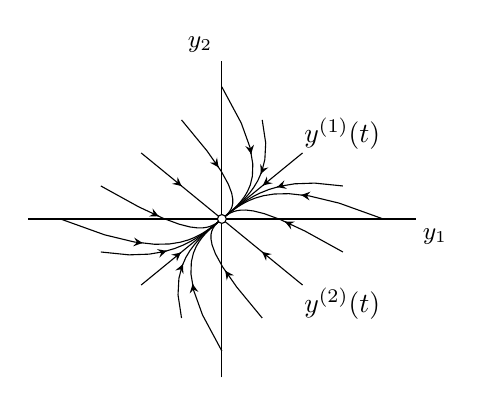
\begin{tikzpicture}
\begin{axis}[small,axis lines*=middle,xtick=\empty,ytick=\empty,xlabel={$y_1$},ylabel={$y_2$},xlabel style={at={(axis description cs:1.05,0.5)}},ylabel style={rotate=-90},ylabel style={at={(axis description cs:0.5,1.05)}}]
\pgfmathsetmacro{\lmtL}{0}
\pgfmathsetmacro{\lmtH}{4}
%
\pgfmathsetmacro{\ca}{1}
\pgfmathsetmacro{\cb}{0}
\addplot[domain=\lmtL:\lmtH]  ({\ca*e^(-x)+\cb*e^(-3*x)},{\ca*e^(-x)-1*\cb*e^(-3*x)})coordinate[pos=0.5](ka)coordinate[pos=0.501](kb)node[pos=0.1,above right]{$\bM{y}^{(1)}(t)$};
\draw[-stealth](ka)--(kb);
\pgfmathsetmacro{\ca}{-1}
\pgfmathsetmacro{\cb}{0}
\addplot[domain=\lmtL:\lmtH]  ({\ca*e^(-x)+\cb*e^(-3*x)},{\ca*e^(-x)-1*\cb*e^(-3*x)})coordinate[pos=0.5](ka)coordinate[pos=0.501](kb);
\draw[-stealth](ka)--(kb);
%
\pgfmathsetmacro{\ca}{1}
\pgfmathsetmacro{\cb}{1}
\addplot[domain=\lmtL:\lmtH]  ({\ca*e^(-x)+\cb*e^(-3*x)},{\ca*e^(-x)-1*\cb*e^(-3*x)})coordinate[pos=0.5](ka)coordinate[pos=0.501](kb);
\draw[-stealth](ka)--(kb);
\pgfmathsetmacro{\ca}{-1}
\pgfmathsetmacro{\cb}{1}
\addplot[domain=\lmtL:\lmtH]  ({\ca*e^(-x)+\cb*e^(-3*x)},{\ca*e^(-x)-1*\cb*e^(-3*x)})coordinate[pos=0.5](ka)coordinate[pos=0.501](kb);
\draw[-stealth](ka)--(kb);
%
\pgfmathsetmacro{\ca}{1}
\pgfmathsetmacro{\cb}{-1}
\addplot[domain=\lmtL:\lmtH]  ({\ca*e^(-x)+\cb*e^(-3*x)},{\ca*e^(-x)-1*\cb*e^(-3*x)})coordinate[pos=0.5](ka)coordinate[pos=0.501](kb);
\draw[-stealth](ka)--(kb);
\pgfmathsetmacro{\ca}{-1}
\pgfmathsetmacro{\cb}{-1}
\addplot[domain=\lmtL:\lmtH]  ({\ca*e^(-x)+\cb*e^(-3*x)},{\ca*e^(-x)-1*\cb*e^(-3*x)})coordinate[pos=0.5](ka)coordinate[pos=0.501](kb);
\draw[-stealth](ka)--(kb);
%
\pgfmathsetmacro{\ca}{0.5}
\pgfmathsetmacro{\cb}{1}
\addplot[domain=\lmtL:\lmtH]  ({\ca*e^(-x)+\cb*e^(-3*x)},{\ca*e^(-x)-1*\cb*e^(-3*x)})coordinate[pos=0.5](ka)coordinate[pos=0.501](kb);
\draw[-stealth](ka)--(kb);
\pgfmathsetmacro{\ca}{-0.5}
\pgfmathsetmacro{\cb}{1}
\addplot[domain=\lmtL:\lmtH]  ({\ca*e^(-x)+\cb*e^(-3*x)},{\ca*e^(-x)-1*\cb*e^(-3*x)})coordinate[pos=0.5](ka)coordinate[pos=0.501](kb);
\draw[-stealth](ka)--(kb);
%
\pgfmathsetmacro{\ca}{1}
\pgfmathsetmacro{\cb}{0.5}
\addplot[domain=\lmtL:\lmtH]  ({\ca*e^(-x)+\cb*e^(-3*x)},{\ca*e^(-x)-1*\cb*e^(-3*x)})coordinate[pos=0.5](ka)coordinate[pos=0.501](kb);
\draw[-stealth](ka)--(kb);
\pgfmathsetmacro{\ca}{1}
\pgfmathsetmacro{\cb}{-0.5}
\addplot[domain=\lmtL:\lmtH]  ({\ca*e^(-x)+\cb*e^(-3*x)},{\ca*e^(-x)-1*\cb*e^(-3*x)})coordinate[pos=0.5](ka)coordinate[pos=0.501](kb);
\draw[-stealth](ka)--(kb);
%
\pgfmathsetmacro{\ca}{-1}
\pgfmathsetmacro{\cb}{0.5}
\addplot[domain=\lmtL:\lmtH]  ({\ca*e^(-x)+\cb*e^(-3*x)},{\ca*e^(-x)-1*\cb*e^(-3*x)})coordinate[pos=0.5](ka)coordinate[pos=0.501](kb);
\draw[-stealth](ka)--(kb);
\pgfmathsetmacro{\ca}{-1}
\pgfmathsetmacro{\cb}{-0.5}
\addplot[domain=\lmtL:\lmtH]  ({\ca*e^(-x)+\cb*e^(-3*x)},{\ca*e^(-x)-1*\cb*e^(-3*x)})coordinate[pos=0.5](ka)coordinate[pos=0.501](kb);
\draw[-stealth](ka)--(kb);
%
\pgfmathsetmacro{\ca}{0}
\pgfmathsetmacro{\cb}{1}
\addplot[domain=\lmtL:\lmtH]  ({\ca*e^(-x)+\cb*e^(-3*x)},{\ca*e^(-x)-1*\cb*e^(-3*x)})coordinate[pos=0.5](ka)coordinate[pos=0.501](kb)node[pos=0.1,below right]{$\bM{y}^{(2)}(t)$};
\draw[-stealth](ka)--(kb);
\pgfmathsetmacro{\ca}{0}
\pgfmathsetmacro{\cb}{-1}
\addplot[domain=\lmtL:\lmtH]  ({\ca*e^(-x)+\cb*e^(-3*x)},{\ca*e^(-x)-1*\cb*e^(-3*x)})coordinate[pos=0.5](ka)coordinate[pos=0.501](kb);
\draw[-stealth](ka)--(kb);
%
\pgfmathsetmacro{\ca}{-0.5}
\pgfmathsetmacro{\cb}{-1}
\addplot[domain=\lmtL:\lmtH]  ({\ca*e^(-x)+\cb*e^(-3*x)},{\ca*e^(-x)-1*\cb*e^(-3*x)})coordinate[pos=0.5](ka)coordinate[pos=0.501](kb);
\draw[-stealth](ka)--(kb);
\pgfmathsetmacro{\ca}{0.5}
\pgfmathsetmacro{\cb}{-1}
\addplot[domain=\lmtL:\lmtH]  ({\ca*e^(-x)+\cb*e^(-3*x)},{\ca*e^(-x)-1*\cb*e^(-3*x)})coordinate[pos=0.5](ka)coordinate[pos=0.501](kb);
\draw[-stealth](ka)--(kb);
%
\addplot[fill=white] plot coordinates {(0,0)}node[ocirc]{};
\end{axis}
\end{tikzpicture}
\caption*{(الف) نظام \حوالہ{مساوات_نظام_خط_حرکت_الف} کے خط حرکت۔ (غیر مناسب جوڑ)}
\end{subfigure}%
\begin{subfigure}{0.5\textwidth}
\centering
\begin{tikzpicture}
\begin{axis}[small,axis lines*=middle,xtick=\empty,ytick=\empty,xlabel={$y_1$},ylabel={$y_2$},xlabel style={at={(axis description cs:1.05,0.5)}},ylabel style={rotate=-90},ylabel style={at={(axis description cs:0.5,1.05)}}]
\pgfmathsetmacro{\lmtL}{-10}
\pgfmathsetmacro{\lmtH}{1}
\pgfmathsetmacro{\ca}{1}
\pgfmathsetmacro{\cb}{1}
\addplot[domain=\lmtL:\lmtH]({\ca*e^x},{\cb*e^x})coordinate[pos=0.5](ka)coordinate[pos=0.501](kb);
\draw[-stealth] (ka)--(kb);
\pgfmathsetmacro{\ca}{1}
\pgfmathsetmacro{\cb}{-1}
\addplot[domain=\lmtL:\lmtH]({\ca*e^x},{\cb*e^x})coordinate[pos=0.5](ka)coordinate[pos=0.501](kb);
\draw[-stealth] (ka)--(kb);
\pgfmathsetmacro{\ca}{-1}
\pgfmathsetmacro{\cb}{1}
\addplot[domain=\lmtL:\lmtH]({\ca*e^x},{\cb*e^x})coordinate[pos=0.5](ka)coordinate[pos=0.501](kb);
\draw[-stealth] (ka)--(kb);
\pgfmathsetmacro{\ca}{-1}
\pgfmathsetmacro{\cb}{-1}
\addplot[domain=\lmtL:\lmtH]({\ca*e^x},{\cb*e^x})coordinate[pos=0.5](ka)coordinate[pos=0.501](kb);
\draw[-stealth] (ka)--(kb);
\pgfmathsetmacro{\ca}{1}
\pgfmathsetmacro{\cb}{0}
\addplot[domain=\lmtL:\lmtH]({\ca*e^x},{\cb*e^x})coordinate[pos=0.5](ka)coordinate[pos=0.501](kb);
\draw[-stealth] (ka)--(kb);
\pgfmathsetmacro{\ca}{-1}
\pgfmathsetmacro{\cb}{0}
\addplot[domain=\lmtL:\lmtH]({\ca*e^x},{\cb*e^x})coordinate[pos=0.5](ka)coordinate[pos=0.501](kb);
\draw[-stealth] (ka)--(kb);
\pgfmathsetmacro{\ca}{0}
\pgfmathsetmacro{\cb}{1}
\addplot[domain=\lmtL:\lmtH]({\ca*e^x},{\cb*e^x})coordinate[pos=0.5](ka)coordinate[pos=0.501](kb);
\draw[-stealth] (ka)--(kb);
\pgfmathsetmacro{\ca}{0}
\pgfmathsetmacro{\cb}{-1}
\addplot[domain=\lmtL:\lmtH]({\ca*e^x},{\cb*e^x})coordinate[pos=0.5](ka)coordinate[pos=0.501](kb);
\draw[-stealth] (ka)--(kb);
%
\addplot[fill=white] plot coordinates {(0,0)}node[ocirc]{};
\end{axis}
\end{tikzpicture}
\caption*{(ب) نظام \حوالہ{مساوات_نظام_مناسب_جوڑ} کے خط حرکت۔ (مناسب جوڑ)}
\end{subfigure}%
\caption{غیر مناسب جوڑ اور مناسب جوڑ۔}
\label{شکل_مثال_نظام_خط_حرکت_غیر_مناسب}
\end{figure}
\انتہا{مثال}
%===================

\جزوحصہء{نظام کا نقطہ فاصل}
ایسا معلوم ہوتا ہے کہ نظام \حوالہ{مساوات_نظام_سطح_مرحلہ_الف} کے تمام \ترچھا{خط حرکت} نقطہ \عددی{\bM{y}=0} سے  گزرتے ہیں۔آئیں دیکھیں کہ ایسا کیوں ہے۔احصاء سے درج ذیل لکھا جا سکتا ہے۔
\begin{align}\label{مساوات_نظام_نقطہ_فاصل_الف}
\frac{\dif y_2}{\dif y_1}=\frac{y_2' \dif t}{y_1'\dif t}=\frac{y_2'}{y_1'}=\frac{a_{21}y_1+a_{22}y_2}{a_{11}y_1+a_{12}y_2}
\end{align}
یوں ماسوائے نقطہ \عددی{P_0:(0,0)} کے، ہر نقطہ \عددی{P:(y_1,y_2)} کے ساتھ  خط حرکت کا مماس \عددی{\tfrac{\dif y_2}{\dif y_1}} منسلک کیا جا سکتا ہے۔نقطہ \عددی{P_0} پر مساوات \حوالہ{مساوات_نظام_نقطہ_فاصل_الف} کا دایاں ہاتھ \ترچھا{نا قابل معلوم} قیمت \عددی{\tfrac{0}{0}} ہو گا۔ایسا نقطہ \عددی{P_0} جس پر
 \عددی{\tfrac{\dif y_2}{\dif y_1}} کی قیمت \ترچھا{نا قابل معلوم} ہو کو نظام \حوالہ{مساوات_نظام_سطح_مرحلہ_الف} کا \اصطلاح{نقطہ فاصل}\فرہنگ{نقطہ فاصل}\حاشیہب{critical point}\فرہنگ{critical point} کہتے ہیں۔

\جزوحصہء{نقطہ فاصل کے پانچ اقسام}
نقطہ فاصل کے قریب، خط حرکت کی جیومیٹریائی صورت کو دیکھ کر \ترچھا{نقطہ فاصل} کی پانچ اقسام بیان کیے جا سکتے ہیں جنہیں \اصطلاح{غیر مناسب جوڑ}\فرہنگ{جوڑ!غیر مناسب}\حاشیہب{improper node}\فرہنگ{node!improper}، \اصطلاح{مناسب جوڑ}\فرہنگ{جوڑ!مناسب}\حاشیہب{proper node}\فرہنگ{node!proper}، \اصطلاح{نقطہ زین}\فرہنگ{نقطہ!زین}\حاشیہب{saddle point}\فرہنگ{point!saddle}\فرہنگ{saddle}، \اصطلاح{وسط}\فرہنگ{وسط}\حاشیہب{center}\فرہنگ{center}  اور  \اصطلاح{نقطہ مرغولہ}\فرہنگ{نقطہ!مرغولہ}\حاشیہب{spiral point}\فرہنگ{point!spiral} کہتے ہیں۔ان کی وضاحت درج ذیل پانچ مثالوں میں کی گئی ہے جہاں ان کی تعریف بھی پیش کی گئی ہیں۔

%===============
\ابتدا{مثال}\شناخت{مثال_نظام_غیر_متناسب_جوڑ}\quad غیر مناسب جوڑ\\
ایسا نقطہ فاصل \عددی{P_0} جس پر، دو \ترچھا{خط حرکت} کے علاوہ، تمام خط حرکت کی مماس کی ایک جیسی تحدیدی سمت پائی جاتی ہو \اصطلاح{غیر مناسب جوڑ} کہلاتا ہے۔دو مختلف خط حرکت کا بھی نقطہ \عددی{P_0} پر تحدیدی سمت پایا جاتا ہے البتہ یہ تحدیدی سمت مختلف ہو گا۔

نظام \حوالہ{مساوات_نظام_خط_حرکت_الف} کا \عددی{\bM{0}} پر غیر مناسب جوڑ پایا جاتا ہے۔چونکہ \عددی{e^{-t}} کی نسبت سے \عددی{e^{-3t}} زیادہ تیزی سے گھٹتی ہے لہٰذا  غیر مناسب جوڑ پر مشترکہ تحدیدی سمت،  \عددی{\bM{x}^{(1)}=[1 \quad 1]^T} کی سمت ہے۔ دو غیر معمولی خط حرکت کی
 سمت \عددی{\bM{x}^{(2)}=[1 \quad -1]^T} اور \عددی{-\bM{x}^{(2)}=[-1\quad 1]^T} کی سمتیں ہیں۔
\انتہا{مثال}
%==================

\ابتدا{مثال}\شناخت{مثال_نظام_مناسب_جوڑ}\quad مناسب جوڑ\\
ایسا نقطہ فاصل \عددی{P_0} جس پر ہر خط حرکت کی  تحدیدی سمت پائی جاتی ہو \اصطلاح{مناسب جوڑ} کہلاتا ہے۔مناسب جوڑ پر ایسا خط حرکت ضرور ہو گا جس کی تحدیدی سمت \عددی{\bM{d}} ہو جہاں \عددی{\bM{d}} کوئی بھی سمت ہو سکتی ہے۔

نظام 
\begin{gather}\label{مساوات_نظام_مناسب_جوڑ}
\begin{aligned}
\bM{y}'=\begin{bmatrix} 1 & 0 \\ 0 &1 \end{bmatrix} \bM{y}
\end{aligned}\quad \implies \quad 
\begin{aligned} 
y_1'&=y_1\\
y_2'&=y_2
\end{aligned}
\end{gather}
کا مناسب جوڑ مبدا پر پایا جاتا ہے۔اس میں فرضی حل \عددی{\bM{y}=\bM{x}e^{\lambda t}} اور اس کا تفرق \عددی{\bM{y}'=\lambda \bM{x}e^{\lambda t}} پر کر کے \عددی{e^{\lambda t}} سے تقسیم کرتے ہوئے \عددی{\bM{A}\bM{x}=\lambda \bM{x}}  یعنی \عددی{(\bM{A}-\lambda\bM{I})\bM{x}=\bM{0}} حاصل ہوتا ہے۔اس کی امتیازی قدر، \عددی{\bM{x} \ne \bM{0}} کی صورت میں، امتیازی مساوات \عددی{(1-\lambda)^2=0} سے  \عددی{\lambda=1}  حاصل ہوتی ہے۔مساوات \عددی{(\bM{A}-\lambda\bM{I})\bM{x}=\bM{0}} کے اجزاء  \عددی{(1-\lambda)x_1=0} اور \عددی{(1-\lambda)x_2=0} میں حاصل امتیازی قدر پر کرتے ہوئے ہم دیکھتے ہیں کہ \عددی{\bM{x} \ne \bM{0}} کے علاوہ امتیازی سمتیہ \عددی{\bM{x}} کی کوئی بھی قیمت چننی جا سکتی ہے۔ یوں \عددی{[1\quad 0]^T} اور \عددی{[0 \quad 1]^T} چنتے ہوئے عمومی حل لکھتے ہیں۔
\begin{gather*}
\begin{aligned}
\bM{y}=c_1\begin{bmatrix}1 \\ 0  \end{bmatrix} e^{t} +c_2\begin{bmatrix} 0 \\ 1 \end{bmatrix} e^{t}
\end{aligned}\quad \implies \quad
\begin{aligned}
y_1&=c_1e^t\\
y_2&=c_2e^t
\end{aligned} \quad \implies \quad
\begin{aligned}
c_1y_2=c_2y_1
\end{aligned}
\end{gather*} 
شکل \حوالہ{شکل_مثال_نظام_خط_حرکت_غیر_مناسب}-ب میں سطح حرکت پر پیکر مرحلہ اور مناسب جوڑ دکھائے گئے ہیں۔ 
\انتہا{مثال}
%====================
\ابتدا{مثال}\شناخت{مثال_نظام_نقطہ_زین}\quad نقطہ زین\\
ایسا نقطہ فاصل \عددی{P_0} جس پر دو عدد آمدی اور دو عدد رخصتی خط حرکت پائے جاتے ہوں \اصطلاح{نقطہ زین}\حاشیہد{نقطہ زین کے خط کی شکل عموماً  گھوڑے کی زین سے مشابہت رکھتی ہے۔اسی سے اس نقطے کو نقطہ زین کہتے ہیں۔}  کہلاتا ہے۔نقطہ فاصل کے قریب بقایا تمام خط حرکت اس نقطے کو نہیں چھوتے۔

نظام
\begin{gather}\label{مساوات_نظام_نقطہ_زین}
\begin{aligned}
\bM{y}'=\begin{bmatrix*}[r] 1&0 \\ 0&-1 \end{bmatrix*} \bM{y}
\end{aligned}\quad \implies \quad
\begin{aligned}
y_1'&=y_1\\ 
y_2'&=-y_2
\end{aligned}
\end{gather}
کا \اصطلاح{نقطہ زین} مبدا پر پایا جاتا ہے۔اس نظام کے امتیازی مساوات \عددی{(-1-\lambda)(1-\lambda)=0} کے جذر \عددی{\lambda_1=1} اور \عددی{\lambda_2=-1} ہیں۔جذر \عددی{\lambda_1} کے لئے \عددی{(\bM{A}-\lambda\bM{I})\bM{x}=\bM{0}} کے دوسرے صف \عددی{0x_1(1-1)x_2=0} میں \عددی{x_1=1} چنتے ہوئے \عددی{x_2=0} ملتا ہے جس سے  امتیازی سمتیہ \عددی{[1\quad 0]^T} حاصل ہوتا ہے۔جذر \عددی{\lambda_2} کے لئے پہلے صف سے امتیازی سمتیہ \عددی{[0\quad 1]^T} حاصل ہوتا ہے۔ان سے عمومی حل لکھتے ہیں۔
\begin{gather}
\begin{aligned}
\bM{y}=c_1\begin{bmatrix}1 \\ 0  \end{bmatrix} e^t+c_2\begin{bmatrix}  0\\1 \end{bmatrix} e^{-t}
\end{aligned} \quad \implies\quad
\begin{aligned}
y_1&=c_1e^t\\
y_2&=c_2e^{-t}
\end{aligned}\quad \implies \quad
\begin{aligned}
y_1y_2=c
\end{aligned}
\end{gather}
عمومی حل \اصطلاح{ہذلولی}\فرہنگ{ہذلولی}\حاشیہب{hyperbolic}\فرہنگ{hyperbolic} ہے جس کو شکل \حوالہ{شکل_مثال_نظام_نقطہ_زین}-الف میں دکھایا گیا ہے۔
\begin{figure}
\centering
\begin{subfigure}{0.5\textwidth}
\centering
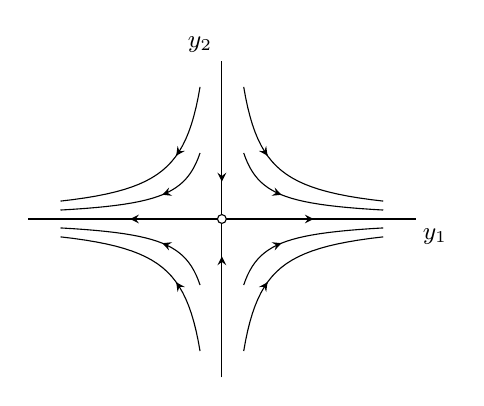
\begin{tikzpicture}
\begin{axis}[small,axis lines*=middle,xtick=\empty,ytick=\empty,xlabel={$y_1$},ylabel={$y_2$},xlabel style={at={(axis description cs:1.05,0.5)}},ylabel style={rotate=-90},ylabel style={at={(axis description cs:0.5,1.05)}}]
\pgfmathsetmacro{\lmtL}{-1}
\pgfmathsetmacro{\lmtH}{1}
%
\pgfmathsetmacro{\ca}{1}
\pgfmathsetmacro{\cb}{1}
\addplot[domain=\lmtL:\lmtH]({\ca*e^x},{\cb*e^(-x)})coordinate[pos=0.5](ka)coordinate[pos=0.501](kb);
\draw[-stealth] (ka)--(kb);
\pgfmathsetmacro{\ca}{-1}
\pgfmathsetmacro{\cb}{1}
\addplot[domain=\lmtL:\lmtH]({\ca*e^x},{\cb*e^(-x)})coordinate[pos=0.5](ka)coordinate[pos=0.501](kb);
\draw[-stealth] (ka)--(kb);
\pgfmathsetmacro{\ca}{1}
\pgfmathsetmacro{\cb}{-1}
\addplot[domain=\lmtL:\lmtH]({\ca*e^x},{\cb*e^(-x)})coordinate[pos=0.5](ka)coordinate[pos=0.501](kb);
\draw[-stealth] (ka)--(kb);
\pgfmathsetmacro{\ca}{-1}
\pgfmathsetmacro{\cb}{-1}
\addplot[domain=\lmtL:\lmtH]({\ca*e^x},{\cb*e^(-x)})coordinate[pos=0.5](ka)coordinate[pos=0.501](kb);
\draw[-stealth] (ka)--(kb);
%
\pgfmathsetmacro{\ca}{1}
\pgfmathsetmacro{\cb}{2}
\addplot[domain=\lmtL:\lmtH]({\ca*e^x},{\cb*e^(-x)})coordinate[pos=0.5](ka)coordinate[pos=0.501](kb);
\draw[-stealth] (ka)--(kb);
\pgfmathsetmacro{\ca}{-1}
\pgfmathsetmacro{\cb}{2}
\addplot[domain=\lmtL:\lmtH]({\ca*e^x},{\cb*e^(-x)})coordinate[pos=0.5](ka)coordinate[pos=0.501](kb);
\draw[-stealth] (ka)--(kb);
\pgfmathsetmacro{\ca}{1}
\pgfmathsetmacro{\cb}{-2}
\addplot[domain=\lmtL:\lmtH]({\ca*e^x},{\cb*e^(-x)})coordinate[pos=0.5](ka)coordinate[pos=0.501](kb);
\draw[-stealth] (ka)--(kb);
\pgfmathsetmacro{\ca}{-1}
\pgfmathsetmacro{\cb}{-2}
\addplot[domain=\lmtL:\lmtH]({\ca*e^x},{\cb*e^(-x)})coordinate[pos=0.5](ka)coordinate[pos=0.501](kb);
\draw[-stealth] (ka)--(kb);
%
\pgfmathsetmacro{\ca}{1}
\pgfmathsetmacro{\cb}{0}
\addplot[domain=\lmtL:\lmtH]({\ca*e^x},{\cb*e^(-x)})coordinate[pos=0.5](ka)coordinate[pos=0.501](kb);
\draw[-stealth] (ka)--(kb);
\pgfmathsetmacro{\ca}{-1}
\pgfmathsetmacro{\cb}{0}
\addplot[domain=\lmtL:\lmtH]({\ca*e^x},{\cb*e^(-x)})coordinate[pos=0.5](ka)coordinate[pos=0.501](kb);
\draw[-stealth] (ka)--(kb);
\pgfmathsetmacro{\ca}{0}
\pgfmathsetmacro{\cb}{-1}
\addplot[domain=\lmtL:\lmtH]({\ca*e^x},{\cb*e^(-x)})coordinate[pos=0.5](ka)coordinate[pos=0.501](kb);
\draw[-stealth] (ka)--(kb);
\pgfmathsetmacro{\ca}{0}
\pgfmathsetmacro{\cb}{1}
\addplot[domain=\lmtL:\lmtH]({\ca*e^x},{\cb*e^(-x)})coordinate[pos=0.5](ka)coordinate[pos=0.501](kb);
\draw[-stealth] (ka)--(kb);
%
\addplot[fill=white] plot coordinates {(0,0)} node[ocirc]{};
\end{axis}
\end{tikzpicture}
\caption*{(الف) نظام \حوالہ{مساوات_نظام_نقطہ_زین} کے خط حرکت۔ (نقطہ زین)}
\end{subfigure}%
\begin{subfigure}{0.5\textwidth}
\centering
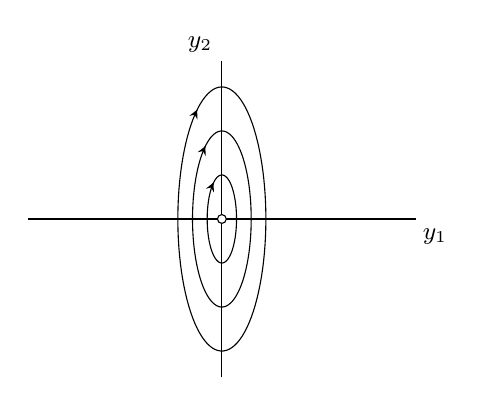
\begin{tikzpicture}
\begin{axis}[small,axis equal,axis lines*=middle,xtick=\empty,ytick=\empty,xlabel={$y_1$},ylabel={$y_2$},xlabel style={at={(axis description cs:1.05,0.5)}},ylabel style={rotate=-90},ylabel style={at={(axis description cs:0.5,1.05)}}]
\pgfmathsetmacro{\ca}{1}
\pgfmathsetmacro{\cb}{1}
\addplot[domain=-60:60,samples=100]({\ca*cos(3*x)+\cb*sin(3*x)},{3*\cb*cos(3*x)-3*\cb*sin(3*x)})coordinate[pos=0.35](ka)coordinate[pos=0.351](kb);
\draw[-stealth] (ka)--(kb);
\pgfmathsetmacro{\ca}{2}
\pgfmathsetmacro{\cb}{2}
\addplot[domain=-60:60,samples=100]({\ca*cos(3*x)+\cb*sin(3*x)},{3*\cb*cos(3*x)-3*\cb*sin(3*x)})coordinate[pos=0.35](ka)coordinate[pos=0.351](kb);
\draw[-stealth] (ka)--(kb);
\pgfmathsetmacro{\ca}{3}
\pgfmathsetmacro{\cb}{3}
\addplot[domain=-60:60,samples=100]({\ca*cos(3*x)+\cb*sin(3*x)},{3*\cb*cos(3*x)-3*\cb*sin(3*x)})coordinate[pos=0.35](ka)coordinate[pos=0.351](kb);
\draw[-stealth] (ka)--(kb);
\addplot[fill=white] plot coordinates {(0,0)} node[ocirc]{};
\end{axis}
\end{tikzpicture}%
\caption*{(ب) نظام \حوالہ{مساوات_نظام_وسط_الف} کے خط حرکت۔ (وسط)}
\end{subfigure}%
\caption{نقطہ زین اور وسط۔}
\label{شکل_مثال_نظام_نقطہ_زین}
\end{figure}
\انتہا{مثال}
%===================
\ابتدا{مثال}\شناخت{مثال_نظام_وسط}\quad وسط\\
ایسا نقطہ فاصل جسے لامتناہی بند خط حرکت گھیرتے ہوں \اصطلاح{وسط} کہلاتا ہے۔

نظام
\begin{gather}\label{مساوات_نظام_وسط_الف}
\begin{aligned}
\bM{y}'=\begin{bmatrix} 0&1\\ -9&0 \end{bmatrix}
\end{aligned}\bM{y} \quad \implies \quad
\begin{aligned}
y_1'&=y_2 \quad (\text{الف})\\
y_2'&=-9y_1\quad (\text{ب})
\end{aligned}
\end{gather}
میں \عددی{\bM{y}=\bM{x}e^{\lambda t}} حل تصور کرتے  ہوئے \عددی{\bM{y}} اور \عددی{\bM{y}'} کو درج بالا میں پر کر کے \عددی{e^{\lambda t}} سے تقسیم کرتے ہوئے  \عددی{(\bM{A}-\lambda \bM{I})\bM{x}=\bM{0}} ملتا ہے۔اس سے \عددی{\bM{x} \ne \bM{0}} کی صورت میں امتیازی مساوات \عددی{\lambda^2+9=0} حاصل ہو گا جس کے امتیازی اقدار \عددی{\lambda_1=3i} اور \عددی{\lambda_2=-3i}  ہیں۔ مساوات \عددی{(\bM{A}-\lambda \bM{I})\bM{x}=\bM{0}} کے پہلے صف میں \عددی{\lambda_1} پر کرتے ہوئے \عددی{x_2=3ix_1} ملتا ہے۔یوں \عددی{x_1=1} چنتے ہوئے \عددی{x_2=3i} حاصل ہو گا جس سے امتیازی سمتیہ \عددی{\bM{x}^{(1)}=[1 \quad 3i]^T} ملتا ہے۔اسی طرح \عددی{\lambda_2} کی مطابقتی امتیازی سمتیہ \عددی{\bM{x}^{(2)}=[1\quad -3i]^T} حاصل ہو گا۔یوں مخلوط عمومی حل لکھتے ہیں۔
\begin{gather}\label{مساوات_نظام_وسط_ب}
\begin{aligned}
\bM{y}=c_1\begin{bmatrix} 1 \\ 3i \end{bmatrix} e^{3i t}+c_2\begin{bmatrix}  1 \\ -3i \end{bmatrix}e^{-3i t}
\end{aligned}\quad \implies \quad
\begin{aligned}
y_1&=c_1e^{3it}+c_2e^{-3it}\\
y_2&=3ic_1e^{3it}-3ic_2e^{-3it}
\end{aligned}
\end{gather}
حقیقی حل \اصطلاح{یولر} مساوات\حاشیہب{$e^{ix}=\cos x+i\sin x\,\,\,$} سے
\begin{align*}
y_1&=A\cos 3t+B\sin 3t\\
y_2&=3B\cos 3t-3A\sin 3t
\end{align*}
 لکھا جا سکتا ہے جہاں \عددی{A=c_1+c_2} اور \عددی{B=i(c_1-c_2)} ہیں۔

حقیقی حل کو مساوات \حوالہ{مساوات_نظام_وسط_الف} سے بھی حاصل کیا جا سکتا ہے۔یوں اگر مساوات \حوالہ{مساوات_نظام_وسط_الف}-الف کے بائیں ہاتھ اور مساوات -ب کے دائیں ہاتھ کو ضرب دیا جائے تو \عددی{-9y_1y_1'} حاصل ہو گا جو مساوات-ب کے بائیں ہاتھ اور مساوات-الف کے دائیں ہاتھ کے حاصل ضرب \عددی{y_2y_2'} کے برابر \عددی{-9y_1y_1'=y_2y_2'} ہو گا۔اس کا تکمل
\begin{align}
\frac{9}{2}y_1^2+\frac{1}{2}y_2^2=c
\end{align}
 ہے جو \عددی{t} سے پاک حقیقی حل ہے۔یہ \اصطلاح{ترخیم}\فرہنگ{ترخیم}\حاشیہب{ellipse}\فرہنگ{ellipse} کی نسل کی مساوات ہے جس کو شکل \حوالہ{شکل_مثال_نظام_نقطہ_زین}-ب  میں دکھایا گیا ہے۔
\انتہا{مثال}
%===================
\ابتدا{مثال}\شناخت{مثال_نظام_نقطہ_مرغولہ}\quad نقطہ مرغولہ\\
ایسا نقطہ فاصل جس کے گرد خط حرکت گھومتے ہوئے نقطہ فاصل تک آن پہنچنے کی کوشش کرے یا نقطہ فاصل سے نکل کر اس نقطے کے گرد گھومتے ہوئے دور ہٹتا جائے \عددی{نقطہ مرغولہ}\فرہنگ{نقطہ مرغولہ}\حاشیہب{spiral point}\فرہنگ{spiral point} کہلاتا ہے۔پہلی صورت میں لمحہ \عددی{t \to \infty} پر خط حرکت نقطہ مرغولہ تک آن پہنچے گا۔

نظام
\begin{gather}\label{مساوات_نظام_مثال_مرغولہ}
\begin{aligned}
\bM{y}'=\begin{bmatrix*}[r] -1&1 \\ -1&-1 \end{bmatrix*}\bM{y}
\end{aligned}\quad \implies \quad
\begin{aligned}
y_1'&=-y_1+y_2 \quad \text{(الف)}\\
y_2'&=-y_1-y_2\quad \text{(ب)}
\end{aligned}
\end{gather}
کا نقطہ مرغولہ مبدا پر پایا جاتا ہے۔امتیازی مساوات \عددی{\lambda^2+2\lambda+2=0} سے امتیازی اقدار \عددی{\lambda_1=-1+i} اور \عددی{\lambda_2=-1-i} حاصل ہوتے ہیں۔مساوات \عددی{(-1-\lambda)x_1+x_2=0} میں امتیازی قدر \عددی{\lambda_1} پر کرتے ہوئے \عددی{-ix_1+x_2=0} ملتا ہے جس میں \عددی{x_1=1} چنتے ہوئے \عددی{x_2=i} حاصل ہوتا ہے اور یوں  \عددی{\lambda_1} کا  مطابقتی امتیازی سمتیہ \عددی{\bM{x}^{(1)}=[1\quad i]^T} ہو گا۔اسی طرح \عددی{\lambda_2} کا مطابقتی امتیازی سمتیہ \عددی{\bM{x}^{(2)}=[1\quad -i]^T} حاصل ہوتا ہے۔  ان سے مخلوط عمومی حل لکھتے ہیں۔
\begin{align*}
\bM{y}=c_1\begin{bmatrix} 1 \\ i \end{bmatrix}e^{(-1+i)t}+c_2\begin{bmatrix*}[r]1\\-i  \end{bmatrix*} e^{(-1-i)t}
\end{align*}
مخلوط عمومی حل سے حقیقی حل حاصل کو \اصطلاح{یولر مساوات} کے ذریعہ حاصل کرتے ہیں۔ہم گزشتہ مثال کی طرح نسبتاً آسان طریقہ استعمال کرتے ہوئے حقیقی حل حاصل کرتے ہیں۔یوں مساوات \حوالہ{مساوات_نظام_مثال_مرغولہ}-الف کو \عددی{y_1} اور مساوات \حوالہ{مساوات_نظام_مثال_مرغولہ}-ب  کو \عددی{y_2} سے ضرب دیتے ہوئے ان کا مجموعہ
\begin{align*}
y_1y_1'+y_2y_2'=-(y_1^2+y_2^2)
\end{align*}
اب ہم نلکی محدد \عددی{r} اور \عددی{t} زیر استعمال لاتے ہیں جہاں \عددی{r^2=y_1^2+y_2^2} ہے۔\عددی{r} کا \عددی{t} کے ساتھ تفرق \عددی{2rr'=2y_1y_1'+2y_2y_2'} ہو گا لہٰذا درج بالا مساوات سے
\begin{align*}
rr'=-r^2,\implies  \frac{\dif r}{r}=-\dif t , \implies r=ce^{-t}
\end{align*}
لکھا جا سکتا ہے۔\عددی{c} کی کسی بھی قیمت کے لئے یہ مرغولی خط کی مساوات ہے جس کو شکل \حوالہ{شکل_نظام_نقطہ_مرغولہ} میں دکھایا گیا ہے۔
\انتہا{مثال}
\begin{figure}
\centering
\begin{tikzpicture}
\begin{axis}[small,axis equal,axis lines*=middle,xtick=\empty,ytick=\empty,xlabel={$y_1$},ylabel={$y_2$},xlabel style={at={(axis description cs:1.05,0.5)}},ylabel style={rotate=-90},ylabel style={at={(axis description cs:0.5,1.05)}}]
\addplot[domain=0:800,samples=100]({x/100*cos(x)},{-x/100*sin(x)})coordinate[pos=0.5](ka)coordinate[pos=0.501](kb);
\draw[stealth-](ka)--(kb);
\addplot[fill=white] plot coordinates {(0,0)}node[ocirc]{};
\end{axis}
\end{tikzpicture}
\caption{نظام \حوالہ{مساوات_نظام_مثال_مرغولہ} کے خط حرکت۔ (نقطہ مرغولہ)}
\label{شکل_نظام_نقطہ_مرغولہ}
\end{figure}
%====================
\ابتدا{مثال}\شناخت{مثال_نظام_انحطاطی_جوڑ_دوسرا_حل}\quad انحطاطی جوڑ\\
بعض اوقات نظام کی امتیازی حل کی اساس نہیں پائی جاتی۔ایسے صورت میں \اصطلاح{انحطاطی جوڑ}\فرہنگ{انحطاطی جوڑ}\حاشیہب{degenerate node}\فرہنگ{node!degenerate} پایا جاتا ہے۔انحطاطی جوڑ، مثال \حوالہ{مثال_نظام_غیر_متناسب_جوڑ} تا مثال \حوالہ{مثال_نظام_نقطہ_زین} کی طرح تشاکلی \عددی{A} (جس میں \عددی{a_{kj}=a_{jk}} ہوتا ہے) کی صورت میں نہیں پایا جائے گا اور نا ہی یہ منحرف تشاکلی (جس میں \عددی{a_{kj}=-a_{jk}} اور \عددی{a_{jj}=0} ہوتا ہے)صورت میں پایا جائے  گا۔ان کے علاوہ، مثال \حوالہ{مثال_نظام_وسط} اور مثال \حوالہ{مثال_نظام_نقطہ_مرغولہ} کی طرح،  کئی دیگر صورتوں میں بھی انحطاطی جوڑ نہیں پایا جاتا ہے۔انحطاطی جوڑ کی صورت میں جو ترکیب استعمال کی جاتی ہے اس کو درج ذیل نظام  کی عمومی حل کے حصول کی مدد سے سمجھتے ہیں۔
\begin{align}\label{مساوات_نظام_انحطاطی_جوڑ_الف}
\bM{y}'=\bM{A}\bM{y}=\begin{bmatrix*}[r] 4 & 1 \\ -1 & 2 \end{bmatrix*}\bM{y}
\end{align}
حل:\عددی{\bM{A}} منحرف تشاکلی نہیں ہے۔ہم اس کا حل \عددی{\bM{y}=\bM{x}e^{\lambda t}} تصور کرتے ہوئے آگے بڑھتے ہیں۔یوں \عددی{\bM{y}} اور \عددی{\bM{y}'} کو درج بالا میں پر کر کے \عددی{e^{\lambda}} سے تقسیم کرتے ہوئے \عددی{(\bM{A}-\lambda\bM{I})\bM{x}=0} ملتا ہے۔ اس کی امتیازی مساوات
\begin{align*}
\abs{\bM{A}-\lambda \bM{I}}=\begin{vmatrix*}[r] 4-\lambda& 1\\-1&2-\lambda \end{vmatrix*}=\lambda^2-6\lambda+9=(\lambda-3)^2=0
\end{align*}
سے دوہرا امتیازی قدر \عددی{\lambda=3} حاصل ہوتا ہے۔مساوات \عددی{(\bM{A}-\lambda\bM{I})\bM{x}=\bM{0}} کے پہلے صف میں \عددی{\lambda=3} پر کرتے ہوئے
\begin{align*}
(4-\lambda)x_1+x_2=0, \quad \implies \quad x_1+x_2=0
\end{align*}
ملتا ہے جس میں \عددی{x_1=1} چننے سے \عددی{x_2=-1} اور یوں امتیازی سمتیہ \عددی{\bM{x}^{(1)}=[1\quad -1]^T} حاصل ہوتا ہے۔

دوسرا حل
\begin{align*}
\bM{y}^{(2)}=\bM{x}te^{\lambda t}+\bM{u}e^{\lambda t}
\end{align*}
 فرض کرتے ہیں جہاں \عددی{\bM{x}=\bM{x}^{(1)}}، \عددی{\lambda=-3} جبکہ \عددی{\bM{u}=[u_1\quad u_2]^T} مستقل  ہے۔(اگر یہاں حصہ \حوالہ{حصہ_سادہ_دو_درجی_مستقل_عددی_سر} کی طرح دوسرا حل صرف \عددی{\bM{x}te^{\lambda t}} پر کیا جائے تو بات نہیں بنتی۔آپ ایسا کر کے تسلی کر لیں۔) فرض کردہ حل اور اس کے تفرق کو مساوات \حوالہ{مساوات_نظام_انحطاطی_جوڑ_الف} میں پر کرتے ہیں۔ 
\begin{align*}
\bM{y}^{(2)'}=\bM{x}e^{\lambda t}+\lambda \bM{x}te^{\lambda t}+\lambda \bM{u}e^{\lambda t}=\bM{A}\bM{y}^{(2)}=\bM{A}\bM{x}te^{\lambda t}+\bM{A}\bM{u}e^{\lambda t}
\end{align*}
دائیں ہاتھ \عددی{\bM{A}\bM{x}=\lambda \bM{x}} ہے لہٰذا دونوں اطراف \عددی{\lambda\bM{x}te^{\lambda t}} کٹ جائے گا۔بقایا مساوات کے دونوں اطراف کو \عددی{e^{\lambda t}} سے تقسیم کرتے ہوئے
\begin{align*}
\bM{x}+\lambda\bM{u}=\bM{A}\bM{u} \quad \implies \quad (\bM{A}-\lambda \bM{I})\bM{u}=\bM{x}
\end{align*}
ملتا ہے۔اس میں \عددی{\bM{x}=\bM{x}^{(1)}} اور \عددی{\lambda=-3} پر کرتے ہیں۔
\begin{gather*}
\begin{aligned}
\begin{bmatrix} 4-3&1 \\ -1&2-3 \end{bmatrix}\bM{u}=\begin{bmatrix*}[r] 1\\ -1  \end{bmatrix*}
\end{aligned}\implies 
\begin{aligned}
u_1+u_2&=1\\
-u_1-u_2&=-1
\end{aligned}
\end{gather*}
انہیں حل کرتے ہوئے یکتا \عددی{\bM{u}} حاصل نہیں کیا جا سکتا ہے۔ یوں \عددی{u_1=0} چننے سے \عددی{u_2=1} لہٰذا \عددی{\bM{u}=[0 \quad 1]^T} حاصل ہوتا ہے۔اس طرح دوسرا حل جو \عددی{\bM{x}^{(1)}=[1\quad -1]^T} سے خطی طور غیر تابع ہو حاصل ہوتا ہے۔انہیں استعمال کرتے ہوئے عمومی حل لکھتے ہیں۔
\begin{align}
\bM{y}=c_1\bM{y}^{(1)}+c_2\bM{y}^{(2)}=c_1\begin{bmatrix*}[r] 1\\-1 \end{bmatrix*}e^{3 t}+c_2\left(\begin{bmatrix*}[r]1\\-1  \end{bmatrix*}t+\begin{bmatrix} 0\\1\end{bmatrix}\right)e^{3t}
\end{align}
ان حل کو شکل \حوالہ{شکل_مساوات_نظام_انحطاطی_جوڑ_الف} میں دکھایا گیا ہے جہاں \عددی{\bM{y}^{(1)}} اور \عددی{\bM{y}^{(2)}} کو موٹی لکیروں سے ظاہر کیا گیا ہے۔یہاں مبدا پر واقع نقطہ فاصل کو عموماً \اصطلاح{انحطاطی جوڑ}\فرہنگ{انحطاطی جوڑ}\فرہنگ{جوڑ!انحطاطی}\حاشیہب{degenerate node}\فرہنگ{degenerate node}\فرہنگ{node!degenerate} کہا جاتا ہے۔
\begin{figure}
\centering
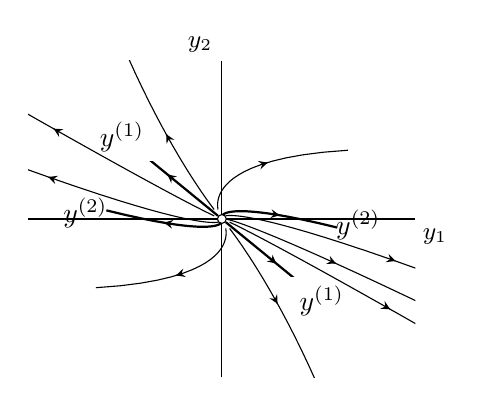
\begin{tikzpicture}
\begin{axis}[small,axis lines*=middle,xmin=-50,xmax=50,ymin=-50,ymax=50,xtick=\empty,ytick=\empty,xlabel={$y_1$},ylabel={$y_2$},xlabel style={at={(axis description cs:1.05,0.5)}},ylabel style={rotate=-90},ylabel style={at={(axis description cs:0.5,1.05)}}]
\pgfmathsetmacro{\lmt}{1.1}
%
\pgfmathsetmacro{\ca}{1}
\pgfmathsetmacro{\cb}{1}
\addplot[domain=0:\lmt]({\ca*e^(3*x)+\cb*x*e^(3*x)},{-\ca*e^(3*x)-\cb*x*e^(3*x)+\cb*e^(3*x)})coordinate[pos=0.5](ka)coordinate[pos=0.501](kb);
\draw[-stealth] (ka)--(kb);
\pgfmathsetmacro{\ca}{1}
\pgfmathsetmacro{\cb}{0}
\addplot[thick,domain=0:\lmt]({\ca*e^(3*x)+\cb*x*e^(3*x)},{-\ca*e^(3*x)-\cb*x*e^(3*x)+\cb*e^(3*x)})coordinate[pos=0.5](ka)coordinate[pos=0.501](kb)node[pos=0.95,fill=white]{$\bM{y}^{(1)}$};
\draw[-stealth] (ka)--(kb);
\pgfmathsetmacro{\ca}{-1}
\pgfmathsetmacro{\cb}{0}
\addplot[thick,domain=0:\lmt]({\ca*e^(3*x)+\cb*x*e^(3*x)},{-\ca*e^(3*x)-\cb*x*e^(3*x)+\cb*e^(3*x)})coordinate[pos=0.5](ka)coordinate[pos=0.501](kb)node[pos=0.95,fill=white]{$\bM{y}^{(1)}$};
\draw[-stealth] (ka)--(kb);
\pgfmathsetmacro{\ca}{0}
\pgfmathsetmacro{\cb}{1}
\addplot[thick,domain=0:\lmt]({\ca*e^(3*x)+\cb*x*e^(3*x)},{-\ca*e^(3*x)-\cb*x*e^(3*x)+\cb*e^(3*x)})coordinate[pos=0.5](ka)coordinate[pos=0.501](kb)node[pos=0.9,right]{$\bM{y}^{(2)}$};
\draw[-stealth] (ka)--(kb);
\pgfmathsetmacro{\ca}{0}
\pgfmathsetmacro{\cb}{-1}
\addplot[thick,domain=0:\lmt]({\ca*e^(3*x)+\cb*x*e^(3*x)},{-\ca*e^(3*x)-\cb*x*e^(3*x)+\cb*e^(3*x)})coordinate[pos=0.5](ka)coordinate[pos=0.501](kb)node[pos=0.9,left]{$\bM{y}^{(2)}$};
\draw[-stealth] (ka)--(kb);
%
\pgfmathsetmacro{\ca}{2}
\pgfmathsetmacro{\cb}{1}
\addplot[domain=0:\lmt]({\ca*e^(3*x)+\cb*x*e^(3*x)},{-\ca*e^(3*x)-\cb*x*e^(3*x)+\cb*e^(3*x)})coordinate[pos=0.5](ka)coordinate[pos=0.501](kb);
\draw[-stealth] (ka)--(kb);
\pgfmathsetmacro{\ca}{-2}
\pgfmathsetmacro{\cb}{1}
\addplot[domain=0:\lmt]({\ca*e^(3*x)+\cb*x*e^(3*x)},{-\ca*e^(3*x)-\cb*x*e^(3*x)+\cb*e^(3*x)})coordinate[pos=0.5](ka)coordinate[pos=0.501](kb);
\draw[-stealth] (ka)--(kb);
\pgfmathsetmacro{\ca}{2}
\pgfmathsetmacro{\cb}{-1}
\addplot[domain=0:\lmt]({\ca*e^(3*x)+\cb*x*e^(3*x)},{-\ca*e^(3*x)-\cb*x*e^(3*x)+\cb*e^(3*x)})coordinate[pos=0.5](ka)coordinate[pos=0.501](kb);
\draw[-stealth] (ka)--(kb);
\pgfmathsetmacro{\ca}{-2}
\pgfmathsetmacro{\cb}{-1}
\addplot[domain=0:\lmt]({\ca*e^(3*x)+\cb*x*e^(3*x)},{-\ca*e^(3*x)-\cb*x*e^(3*x)+\cb*e^(3*x)})coordinate[pos=0.5](ka)coordinate[pos=0.501](kb);
\draw[-stealth] (ka)--(kb);
%
\pgfmathsetmacro{\ca}{1}
\pgfmathsetmacro{\cb}{2}
\addplot[domain=0:\lmt]({\ca*e^(3*x)+\cb*x*e^(3*x)},{-\ca*e^(3*x)-\cb*x*e^(3*x)+\cb*e^(3*x)})coordinate[pos=0.5](ka)coordinate[pos=0.501](kb);
\draw[-stealth] (ka)--(kb);
\pgfmathsetmacro{\ca}{-1}
\pgfmathsetmacro{\cb}{2}
\addplot[domain=0:\lmt]({\ca*e^(3*x)+\cb*x*e^(3*x)},{-\ca*e^(3*x)-\cb*x*e^(3*x)+\cb*e^(3*x)})coordinate[pos=0.5](ka)coordinate[pos=0.501](kb);
\draw[-stealth] (ka)--(kb);
\pgfmathsetmacro{\ca}{1}
\pgfmathsetmacro{\cb}{-2}
\addplot[domain=0:\lmt]({\ca*e^(3*x)+\cb*x*e^(3*x)},{-\ca*e^(3*x)-\cb*x*e^(3*x)+\cb*e^(3*x)})coordinate[pos=0.5](ka)coordinate[pos=0.501](kb);
\draw[-stealth] (ka)--(kb);
\pgfmathsetmacro{\ca}{-1}
\pgfmathsetmacro{\cb}{-2}
\addplot[domain=0:\lmt]({\ca*e^(3*x)+\cb*x*e^(3*x)},{-\ca*e^(3*x)-\cb*x*e^(3*x)+\cb*e^(3*x)})coordinate[pos=0.5](ka)coordinate[pos=0.501](kb);
\draw[-stealth] (ka)--(kb);
%
\addplot[fill=white] plot coordinates {(0,0)}node[ocirc]{};
\end{axis}
\end{tikzpicture}
\caption{نظام \حوالہ{مساوات_نظام_انحطاطی_جوڑ_الف} کے خط حرکت۔ (انحطاطی جوڑ)}
\label{شکل_مساوات_نظام_انحطاطی_جوڑ_الف}
\end{figure}
\انتہا{مثال}
%=======================

یہاں بتلاتا چلوں کہ، تین یا تین سے زائد تفرقی مساوات کے نظام جس کے سہ گنّا امتیازی قدر  اور  ایک عدد خطی طور غیر تابع امتیازی سمتیہ پایا جاتا ہو کا دوسرا خطی طور غیر تابع امتیازی سمتیہ مثال \حوالہ{مثال_نظام_انحطاطی_جوڑ_دوسرا_حل} کی طرح حاصل کیا جائے گا جبکہ اس کا تیسرا خطی طور غیر تابع امتیازی سمتیہ درج ذیل فرض کرتے ہوئے حاصل ہو گا
\begin{align}
\bM{y}^{(3)}=\frac{1}{2}\bM{x}t^2e^{\lambda t}+\bM{u}te^{\lambda t}+\bM{v}e^{\lambda t}
\end{align}
جہاں \عددی{\bM{v}} کو
\begin{align}
\bM{u}+\lambda \bM{v}=\bM{A}\bM{v}
\end{align}
 سے حاصل کیا جاتا ہے۔یہاں \عددی{\bM{u}} دوسرے خطی طور امتیازی سمتیہ سے لیا جائے گا۔ 
%================================
\حصہء{سوالات}
سوال \حوالہ{سوال_نظام_امتیازی_مسائل_الف} تا سوال \حوالہ{سوال_نظام_امتیازی_مسائل_ب} کے حل دریافت کریں۔ 

%============
\ابتدا{سوال}\شناخت{سوال_نظام_امتیازی_مسائل_الف}
\begin{align*}
y_1'&=-y_1+y_2\\
y_2'&=3y_1+y_2
\end{align*}
جوابات:\عددی{y_1=c_1e^{-2t}+c_2e^{2t}}، \عددی{y_2=-c_1e^{-2t}+3c_2e^{2t}}
\انتہا{سوال}
%=============
\ابتدا{سوال}
\begin{align*}
y_1'&=6y_1+y_2\\
y_2'&=-6y_1+y_2
\end{align*}
جوابات:\عددی{y_1=c_1e^{3t}+c_2e^{4t}}، \عددی{y_2=-3c_1e^{3t}-2c_2e^{4t}}
\انتہا{سوال}
%=============
\ابتدا{سوال}
\begin{align*}
y_1'&=y_1+y_2\\
y_2'&=2y_1+2y_2
\end{align*}
جوابات:\عددی{y_1=c_1+c_2e^{3t}}، \عددی{y_2=-c_1+2c_2e^{3t}}
\انتہا{سوال}
%=============
\ابتدا{سوال}
\begin{align*}
y_1'&=-y_1+2y_2\\
y_2'&=-2y_1+3y_2
\end{align*}
جواب:\عددی{\bM{y}=c_1\begin{bmatrix} 1\\1 \end{bmatrix}e^t+c_2\begin{bmatrix} 1\\1 \end{bmatrix}te^{t}+c_2\begin{bmatrix} 1 \\ \tfrac{3}{2}  \end{bmatrix} e^t} جہاں \عددی{u_1=1} چننا گیا ہے۔
\انتہا{سوال}
%====================
\ابتدا{سوال}
\begin{align*}
y_1'&=3y_1+3y_2\\
y_2'&=-\frac{4}{3}y_1-2y_2
\end{align*}
جوابات:\عددی{y_1=c_1e^{2t}+c_2e^{-t}}، \عددی{y_2=-\tfrac{1}{3}c_1e^{2t}-\tfrac{4}{3}c_2e^{-t}}
\انتہا{سوال}
%=============
\ابتدا{سوال}
\begin{align*}
y_1'&=-12y_1-5y_2\\
y_2'&=\frac{56}{3}y_1+3y_2
\end{align*}
جوابات:\عددی{y_1=c_1e^{-5t}+c_2e^{-4t}}، \عددی{y_2=-\tfrac{7}{5}c_1e^{-5t}-\tfrac{8}{5}c_2e^{-4t}}
\انتہا{سوال}
%=============
\ابتدا{سوال}
\begin{align*}
y_1'&=-y_1+2y_2\\
y_2'&=-9y_1+5y_2
\end{align*}
جوابات:
\begin{align*}
\bM{y}=c_1\begin{bmatrix} 1 \\ \tfrac{3}{2}(1-i) \end{bmatrix} e^{(2-i3)t}+c_2\begin{bmatrix} 1\\ \tfrac{3}{2}(1+i) \end{bmatrix} e^{(2+i3)t}
\end{align*}
جس سے \اصطلاح{یولر مساوات} کی مدد سے درج ذیل حقیقی حل لکھا جا سکتا ہے جہاں \عددی{A=c_1+c_2} اور \عددی{B=-i(c_1-c_2)} ہیں۔
\begin{align*}
y_1&=e^{2t}(A\cos 3t+B\sin 3t)\\
y_2&=\tfrac{3}{2}e^{2t}[(B+A)\cos 3t+(B-A)\sin 3t]
\end{align*}
\انتہا{سوال}
%=============
\ابتدا{سوال}
\begin{align*}
y_1'&=2y_2\\
y_2'&=-y_1+3y_3\\
y_3'&=-y_2
\end{align*}
جوابات:
\begin{align*}
\bM{y}=c_1\begin{bmatrix}1\\[0.5ex] -i\tfrac{\sqrt{5}}{2} \\[0.5ex] -\tfrac{1}{2} \end{bmatrix}e^{-i\sqrt{5}t}+c_2\begin{bmatrix} 1\\[0.5ex]  i\tfrac{\sqrt{5}}{2}\\[0.5ex] -\tfrac{1}{2} \end{bmatrix} e^{i\sqrt{5}t}+c_3\begin{bmatrix}1\\[0.5ex] 0 \\[0.5ex]  \tfrac{1}{3}  \end{bmatrix}
\end{align*}
\انتہا{سوال}
%=============
\ابتدا{سوال}
\begin{align*}
y_1'&=11y_1+2y_2\\
y_2'&=-4y_1+5y_2
\end{align*}
جوابات:\عددی{y_1=c_1e^{9t}+c_2e^{7t}}، \عددی{y_2=-c_1e^{9t}-2c_2e^{7t}}
\انتہا{سوال}
%=============
\ابتدا{سوال}\شناخت{سوال_نظام_امتیازی_مسائل_ب}
\begin{align*}
y_1'&=y_1-10y_2-14y_3\\
y_2'&=-10y_1+10y_2-4y_3\\
y_3&=-14y_1-4y_2-2y_3
\end{align*}
جوابات:
\begin{align*}
\bM{y}=c_1\begin{bmatrix*}[r] 1 \\ -1 \\ -\tfrac{1}{2} \end{bmatrix*}e^{18t}+c_2\begin{bmatrix*}[r] 1\\2\\-2 \end{bmatrix*} e^{9t}+c_3\begin{bmatrix*}[r] 1\\ \tfrac{1}{2}\\1 \end{bmatrix*} e^{-18t}
\end{align*}
\انتہا{سوال}
%=============

سوال \حوالہ{سوال_نظام_امتیازی_ابتدائی_قیمت_مسائل_الف} تا سوال \حوالہ{سوال_نظام_امتیازی_ابتدائی_قیمت_مسائل_ب} ابتدائی قیمت مسائل ہیں۔انہیں حل کریں۔

%============
\ابتدا{سوال}\شناخت{سوال_نظام_امتیازی_ابتدائی_قیمت_مسائل_الف}
\begin{align*}
y_1'&=-6y_1+2y_2\\
y_2'&=-12y_1+5y_2\\
y_1(0)&=2,\quad y_2(0)=1
\end{align*}
جوابات:\عددی{y_1=\tfrac{14}{5}e^{-3t}-\tfrac{4}{5}e^{2t}}، \عددی{y_2=\tfrac{21}{5}e^{-3t}-\tfrac{16}{5}e^{2t}}
\انتہا{سوال}
%=================
\ابتدا{سوال}
\begin{align*}
y_1'&=-\frac{11}{3}y_1+y_2\\
y_2'&=-\frac{32}{3}y_1+3y_2\\
y_1(0)&=-10,\quad y_2(0)=2
\end{align*}
جوابات:\عددی{y_1=\tfrac{43}{2}e^{\tfrac{t}{3}}-\tfrac{63}{2}e^{-t}}، \عددی{y_2=86e^{\tfrac{t}{3}}-84e^{-t}}
\انتہا{سوال}
%=================
\ابتدا{سوال}
\begin{align*}
y_1'&=-y_1-3y_2\\
y_2'&=\frac{5}{3}y_1+5y_2\\
y_1(0)&=2,\quad y_2(0)=-1
\end{align*}
جوابات:\عددی{y_1=\tfrac{1}{4}e^{4t}+\tfrac{7}{4}}، \عددی{y_2=-\tfrac{5}{12}e^{4t}-\tfrac{7}{12}}
\انتہا{سوال}
%=================
\ابتدا{سوال}
\begin{align*}
y_1'&=y_2\\
y_2'&=y_1\\
y_1(0)&=-1,\quad y_2(0)=2
\end{align*}
جوابات:\عددی{y_1=\tfrac{1}{2}e^{t}-\tfrac{3}{2}e^{-t}}، \عددی{y_2=\tfrac{1}{2}e^{t}+\tfrac{3}{2}e^{-t}}
\انتہا{سوال}
%=================
\ابتدا{سوال}
\begin{align*}
y_1'&=-y_2\\
y_2'&=y_1\\
y_1(0)&=0,\quad y_2(0)=-1
\end{align*}
جوابات:\عددی{y_1=\sin t}، \عددی{y_2=-\cos t}
\انتہا{سوال}
%=================
\ابتدا{سوال}\شناخت{سوال_نظام_امتیازی_ابتدائی_قیمت_مسائل_ب}
\begin{align*}
y_1'&=-y_1+y_2\\
y_2'&=y_1-y_2\\
y_1(0)&=-2,\quad y_2(0)=1
\end{align*}
جوابات:\عددی{y_1=-\tfrac{3}{2}e^{-2t}-\tfrac{1}{2}}، \عددی{y_2=\tfrac{3}{2}e^{-2t}-\tfrac{1}{2}}
\انتہا{سوال}
%=================
سوال \حوالہ{سوال_نظام_امتیازی_تبادلہ_الف} تا سوال \حوالہ{سوال_نظام_امتیازی_تبادلہ_ب} میں تفرقی مساوات تبدیل کرنے کو کہا گیا ہے۔ان میں \عددی{y_1} کی عمومی مساوات دریافت کریں۔

%==============
\ابتدا{سوال}\شناخت{سوال_نظام_امتیازی_تبادلہ_الف}
آپ نے گزارش ہے کہ سوال \حوالہ{سوال_نظام_امتیازی_مسائل_الف} کے نظام سے دو رتبی مساوات حاصل کریں جس میں صرف \عددی{y_1} اور اس کے تفرق پائے جاتے ہوں۔حاصل دو رتبی مساوات  کو حل کرتے ہوئے \عددی{y_1} کی عمومی حل دریافت کریں۔

جوابات: پہلی مساوات کا تفرق لیتے ہوئے \عددی{y_1''=-y_1'+y_2'} ملتا ہے  جس میں \عددی{y_2'} کی جگہ دوسری مساوات پر کرتے ہوئے \عددی{y_1''=-y_1'+(3y_1+y_2)} حاصل ہوتا ہے۔اب پہلی مساوات سے \عددی{y_2} اس میں پر کریں۔یوں \عددی{y_1''=-y_1'+3y_1+(y_1'+y_1)} یعنی \عددی{y_1''=4y_1} ملتا ہے۔اس کا عمومی حل
 \عددی{y_1=c_1e^{-2t}+c_2e^{2t}} ہے۔
\انتہا{سوال}
%====================
\ابتدا{سوال}\شناخت{سوال_نظام_امتیازی_تبادلہ_ب}
یہاں سوال \حوالہ{سوال_نظام_امتیازی_ابتدائی_قیمت_مسائل_ب} کے نظام سے دو رتبی مساوات حاصل کریں جس میں صرف \عددی{y_1} اور اس کے تفرق پائے جاتے ہوں۔حاصل دو رتبی مساوات  کو حل کرتے ہوئے \عددی{y_1} کی عمومی حل دریافت کریں۔

جوابات:\عددی{y_1''+2y_1'=0}، \عددی{y_1=c_1+c_2e^{-2t}}
\انتہا{سوال}
%====================
\ابتدا{سوال}\شناخت{سوال_نظام_امتیازی_ٹینکی}\quad ٹینکیوں میں محلول کی تیاری\\
دو عدد ٹینکیاں شکل \حوالہ{شکل_سوال_نظام_امتیازی_ٹینکی} میں دکھائی گئی ہیں۔ٹینکی الف میں ابتدائی طور پر دو سو \عددی{(200)} لٹر پانی پایا جاتا ہے جس میں  پچاس  \عددی{(50)} کلو گرام نمک حل کی گئی ہے۔ٹینکی ب میں ابتدائی طور پر دو سو \عددی{(200)} لٹر خالص پانی پایا جاتا ہے۔پانی کے نظام کو شکل میں دکھایا گیا ہے۔ٹینکی الف میں نمک کی مقدار \عددی{y_1} اور ٹینکی ب میں نمک کی مقدار \عددی{y_2} کے لئے تفرقی مساوات کا نظام لکھیں۔اس نظام کو حل کریں۔

\begin{figure}
\centering
\begin{tikzpicture}
\draw(0,0) rectangle ++(-3/4*\x,\y);
\draw(\x,0) rectangle ++(3/4*\x,\y);
\draw(0,\y/4) rectangle ++(\x,\y/8);
\draw(0,3/4*\y) rectangle ++(\x,-\y/8);
\draw(-3/8*\x,\y/2)node[]{\RL{ٹینکی ب}};
\draw(\x+3/8*\x,\y/2)node[]{\RL{ٹینکی الف}};
\draw[latex-] (\x/4,\y/4+\y/16)--++(\x/2,0);
\draw[-latex] (\x/4,3/4*\y-\y/16)--++(\x/2,0);
\draw(\x/2,\y/4)node[below]{\RL{$12$ لٹر فی منٹ}};
\draw(\x/2,3/4*\y)node[above]{\RL{$2$ لٹر فی منٹ}};
\draw(-3/4*\x,1/8*\y) rectangle ++(-3/4*\x,\y/8);
\draw(\x+3/4*\x,7/8*\y) rectangle ++(3/4*\x,-\y/8);
\draw[-latex] (\x+3/4*\x+3/4*\x-\x/5,7/8*\y-\y/16)--++(-\x/3,0)node[pos=0.5,shift={(0,0.4)}]{\RL{$10$ لٹر فی منٹ}}node[pos=0.5,shift={(0,-0.4)}]{\RL{خالص پانی}};
\draw[latex-] (-3/4*\x-3/4*\x+\x/5,1/8*\y+\y/16)--++(\x/3,0)node[pos=0.5,shift={(0,0.4)}]{\RL{$10$ لٹر فی منٹ}};
\end{tikzpicture}
\caption{سوال \حوالہ{سوال_نظام_امتیازی_ٹینکی} میں ٹینکیوں کا نظام۔}
\label{شکل_سوال_نظام_امتیازی_ٹینکی}
\end{figure}%

جوابات:\عددی{y_1'=-\tfrac{12}{200}y_1+\tfrac{2}{200}y_2}، \عددی{y_2'=\tfrac{12}{200}y_1-\tfrac{12}{200}y_2}،\\
\عددی{y_1=50e^{-\tfrac{3}{50}t}\cosh \tfrac{\sqrt{6}t}{100}}، \عددی{y_2=50\sqrt{6}e^{-\tfrac{3}{50}t}\sinh \tfrac{\sqrt{6}t}{100}}
\انتہا{سوال}
%==========================
\ابتدا{سوال}\شناخت{سوال_نظام_امتیازی_برقی_دور}
مزاحمت، امالہ اور برق گیر کو شکل \حوالہ{شکل_سوال_نظام_امتیازی_برقی_دور} میں متوازی جڑا دکھایا گیا ہے۔اس کی نمونہ کشی کرتے ہوئے تفرقی مساوات لکھتے ہوئے تفرقی مساوات کا نظام حاصل کریں۔\عددی{L=\SI{2}{\henry}}، \عددی{R=\SI{1}{\ohm}} اور \عددی{C=\SI{0.5}{\farad}} کی صورت میں \عددی{I_1} اور \عددی{I_2} کا عمومی حل دریافت کریں۔
\begin{figure}
\centering
\begin{tikzpicture}
\draw(0,0) to [inductor,l={$L$}]++(0,\yy) to [short]++(2*\xx,0) to [capacitor,l={$C$}]++(0,-\yy) to [short]++(-2*\xx,0);
\draw(\xx,0) to [resistor,*-*,l={$R$}]++(0,\yy); 
%currents
\draw[stealth-] ([shift={(-150:\xx/5)}]\xx/2,\yy/2) arc (-150:150:\xx/5);
\draw[stealth-] ([shift={(-150:\xx/5)}]\xx+\xx/2,\yy/2) arc (-150:150:\xx/5);
\draw (\xx/2,\yy/2)node{$I_1$};
\draw (\xx+\xx/2,\yy/2)node{$I_2$};
\end{tikzpicture}
\caption{سوال \حوالہ{سوال_نظام_امتیازی_برقی_دور} کا دور۔}
\label{شکل_سوال_نظام_امتیازی_برقی_دور}
\end{figure}

جوابات:
\begin{align*}
LI_1'+(I_1-I_2)R&=0\\
\tfrac{1}{C}\int I_2 \dif t+(I_2-I_1)R&=0
\end{align*}
پہلی مساوات سے نظام کی ایک مساوات \عددی{I_1'=-\tfrac{R}{L}I_1+\tfrac{R}{L}I_2} ملتی ہے۔دوسری مساوات کا تفرق لیتے ہوئے ترتیب دے کر آخر میں پہلی مساوات سے \عددی{I_1'} پر کرتے ہیں
\begin{align*}
\frac{I_2}{C}+(I_2'-I_1')R=0 \implies I_2'=I_1'-\frac{I_2}{RC} \implies  I_2'=\frac{R}{L}(-I_1+I_2)-\frac{I_2}{RC}
\end{align*}
جس سے تفرقی مساوات کے نظام کی دوسری مساوات \عددی{I_2'=-\tfrac{R}{L}I_1+(\tfrac{R}{L}-\tfrac{1}{RC})I_2} حاصل ہوتی ہے۔دی گئی قیمتیں پر کرتے ہوئے تفرقی مساوات کا نظام 
\begin{align*}
I_1'&=-0.5I_1+0.5I_2\\
I_2'&=-0.5I_1-1.5I_2
\end{align*}
ہو گا جس کا دوہرا جذر \عددی{\lambda=-1} اور مطابقتی امتیازی سمتیہ \عددی{\bM{x}^{(1)}=[1\quad -1]^T} ہے۔یوں مثال \حوالہ{مثال_نظام_انحطاطی_جوڑ_دوسرا_حل} کی طرز پر  حل کرتے ہوئے \عددی{u_1=1} چننے سے \عددی{u_2=1} حاصل ہوتا ہے لہٰذا درج ذیل اساس حاصل کرتے ہیں
\begin{align*}
\bM{y}^{(1)}&=\begin{bmatrix*}[r] 1\\ -1 \end{bmatrix*} e^{-t}\\
\bM{y}^{(2)}&=\begin{bmatrix*}[r] 1\\ -1 \end{bmatrix*} te^{-t}+\begin{bmatrix} 1\\1 \end{bmatrix}e^{-t}
\end{align*}
جس سے  عمومی حل \عددی{\bM{I}=c_1\bM{y}^{(1)}+c_2\bM{y}^{(2)}} لکھا جائے گا۔
\انتہا{سوال}
%==========================

\حصہ{نقطہ فاصل کے جانچ پڑتال کا مسلمہ معیار۔استحکام}
ہم مستقل عددی سر والے متجانس خطی نظام \حوالہ{مساوات_نظام_جانچ_نقطہ_فاصل_الف} پر گفتگو جاری رکھتے ہیں۔
\begin{gather}\label{مساوات_نظام_جانچ_نقطہ_فاصل_الف}
\begin{aligned}
\bM{y}'=\begin{bmatrix} a_{11} & a_{12} \\ a_{21} & a_{22} \end{bmatrix} \bM{y}
\end{aligned}, \quad \implies \quad 
\begin{aligned}
y_1'&=a_{11}y_1+a_{12}y_2\\
y_2'&=a_{21}y_1'+a_{22}y_2
\end{aligned}
\end{gather}
اب تک  حصہ \حوالہ{حصہ_نظام_مستقل_عددی_سر_نظام} میں ہم نے دیکھا کہ نسل حل \عددی{\bM{y}=[y_1(t)\quad y_2(t)]^T} کے خطوط کو \عددی{y_1 y_2} \اصطلاح{سطح حرکت} پر کھینچتے ہوئے عمومی جائزہ لیا جا سکتا ہے۔ اس سطح پر منحنی کو نظام \حوالہ{مساوات_نظام_جانچ_نقطہ_فاصل_الف} کا \اصطلاح{خط حرکت} کہتے ہیں۔تمام خط حرکت کو ملا کر \اصطلاح{پیکر مرحلہ} حاصل ہوتا ہے۔

ہم دیکھ چکے کہ \عددی{\bM{y}=\bM{x}e^{\lambda t}} کو حل تصور کرتے ہوئے مساوات \حوالہ{مساوات_نظام_جانچ_نقطہ_فاصل_الف} میں پر کرتے ہوئے
\begin{align*}
\bM{y}'=\lambda \bM{x}e^{\lambda t}=\bM{A}\bM{y}=\bM{A}\bM{x}e^{\lambda t}
\end{align*}
لکھا جا سکتا ہے جس کو \عددی{e^{\lambda t}} سے تقسیم کرتے ہوئے
\begin{align}\label{مساوات_نظام_جانچ_نقطہ_فاصل_ب}
\bM{A}\bM{x}=\lambda \bM{x}
\end{align}
ملتا ہے۔یوں \عددی{\lambda} قالب \عددی{\bM{A}}  کا امتیازی قدر اور \عددی{\bM{x}} مطابقتی امتیازی سمتیہ ہونے کی صورت میں  \عددی{\bM{y}(t)} مساوات \حوالہ{مساوات_نظام_جانچ_نقطہ_فاصل_الف} کا (غیر صفر) حل ہو گا۔

گزشتہ حصے کے مثالوں سے واضح ہے کہ پیکر مرحلہ کی صورت کا دارومدار بڑی حد تک نظام \حوالہ{مساوات_نظام_جانچ_نقطہ_فاصل_الف} کی \اصطلاح{نقطہ فاصل} کی قسم پر منحصر ہے جہاں نقطہ فاصل سے مراد ایسا نقطہ ہے جہاں \عددی{\tfrac{\dif y_1}{\dif y_2}} نا قابل معلوم قیمت \عددی{\tfrac{0}{0}} ہو۔[مساوات \حوالہ{مساوات_نظام_نقطہ_فاصل_الف} دیکھیں۔]
\begin{align}\label{مساوات_نظام_جانچ_نقطہ_فاصل_پ}
\frac{\dif y_2}{\dif y_1}=\frac{y_2' \dif t}{y_1'\dif t}=\frac{y_2'}{y_1'}=\frac{a_{21}y_1+a_{22}y_2}{a_{11}y_1+a_{12}y_2}
\end{align}
حصہ \حوالہ{حصہ_نظام_مستقل_عددی_سر_نظام}  سے ہم یہ بھی جانتے ہیں نقطہ فاصل کے کئی اقسام پائے جاتے ہیں۔

موجودہ حصے میں ہم دیکھیں گے کہ  نقطہ فاصل کی قسم  کا تعلق امتیازی قدر سے ہے جو امتیازی مساوات
\begin{align}\label{مساوات_نظام_جانچ_نقطہ_فاصل_ت}
\abs{\bM{A}-\lambda \bM{I}}=\begin{vmatrix*}[r] a_{11}-\lambda & a_{12} \\a_{21}&a_{22}-\lambda\end{vmatrix*}=\lambda^2-(a_{11}+a_{22})\lambda+a_{11}a_{22}-a_{12}a_{21}=0
\end{align}
کے حل \عددی{\lambda_1} اور \عددی{\lambda_2} ہیں۔امتیازی مساوات دو درجی مساوات \عددی{\lambda^2-p\lambda+q=0} ہے جس کے عددی سر \عددی{p}،  \عددی{q} اور \اصطلاح{ممیز}\فرہنگ{ممیز}\حاشیہب{discriminant}\فرہنگ{discriminant} \عددی{\Delta} درج ذیل ہیں۔
\begin{align}\label{مساوات_نظام_جانچ_نقطہ_فاصل_ٹ}
p=a_{11}+a_{22}, \quad q=a_{11}a_{22}-a_{12}a_{21},\quad \Delta=p^2-4q
\end{align}
دو درجی مساوات کے حل الجبرا کی مدد سے \عددی{\lambda=\tfrac{1}{2}(p+\mp\sqrt{p^2-4q})} یعنی
\begin{align}\label{مساوات_نظام_جانچ_نقطہ_فاصل_ث}
\lambda_1=\frac{1}{2}(p+\sqrt{\Delta}),\quad \lambda_2=\frac{1}{2}(p-\sqrt{\Delta})
\end{align} 
لکھتے ہیں۔ان امتیازی اقدار کو استعمال کرتے ہوئے امتیازی مساوات کو اجزائے ضربی کی صورت 
\begin{align*}
(\lambda-\lambda_1)(\lambda-\lambda_2)=\lambda^2-(\lambda_1+\lambda_2)+\lambda_1\lambda_2=0
\end{align*}
میں لکھا جا سکتا ہے  جہاں سے ظاہر ہے کہ \عددی{p} امتیازی اقدار کا مجموعہ ہے جبکہ \عددی{q} ان کا حاصل ضرب ہے۔اسی طرح مساوات \حوالہ{مساوات_نظام_جانچ_نقطہ_فاصل_ث} کی مدد سے \عددی{\lambda_1-\lambda_2=\sqrt{\Delta}} لکھا جا سکتا ہے۔
\begin{align}
p=\lambda_1+\lambda_2,\quad q=\lambda_1\lambda_2,\quad \Delta=(\lambda_1-\lambda_2)^2
\end{align}
ان نتائج سے  نقطہ فاصل کی جانچ کے اصول طے کئے جا سکتے ہیں جنہیں جدول \حوالہ{جدول_نظام_نقطہ_فاصل_اصول_جانچ} میں پیش کیا گیا ہے۔ان اصولوں کو اسی حصے میں اخذ کیا جائے گا۔
\begin{table}
\caption{امتیازی قدر سے نقطہ فاصل کی درجہ بندی۔}
\label{جدول_نظام_نقطہ_فاصل_اصول_جانچ}
\centering
\begin{tabular}{rcccr}
نام& $p=\lambda_1+\lambda_2$&$q=\lambda_1\lambda_2$&$\Delta=(\lambda_1-\lambda_2)^2$&$\lambda_1$ اور $\lambda_2$  پر تبصرہ\\
\hline
(الف) جوڑ & & \عددی{q >0} & \عددی{\Delta \ge 0} & حقیقی۔یکساں علامتیں\\
(ب) نقطہ زین & & \عددی{q<0}& & حقیقی۔آپس میں الٹ علامتیں\\
(پ) وسط & \عددی{p=0} & \عددی{q>0}&& خالص خیالی عدد (حقیقی جزو صفر ہے)\\
(ت) نقطہ مرغولہ & \عددی{p \ne 0} & & \عددی{\Delta <0}& مخلوط عدد (حقیقی اور خیالی اجزاء غیر صفر ہیں)
\end{tabular}
\end{table}
%===================

\جزوحصہء{استحکام}
نقطہ فاصل کی درجہ بندی ان کی \اصطلاح{استحکام}\فرہنگ{استحکام}\حاشیہب{stability}\فرہنگ{stability} کی بنیاد پر بھی کی جا سکتی ہے۔انجینئری کے علاوہ دیگر شعبوں میں بھی  استحکام نہایت اہم تصور ہے۔مستحکم نظام میں کسی لمحے پر معمولی تبدیلی یا خلل سے بعد کے تمام لمحات پر معمولی خلل ہی پایا جاتا ہے۔ نقطہ فاصل کے لئے درج ذیل تصورات اہم ہیں۔
%============

\ابتدا{تعریف}\quad مستحکم، غیر مستحکم، مستحکم اور جاذب\\
اگر نظام \حوالہ{مساوات_نظام_جانچ_نقطہ_فاصل_الف} کے نقطہ فاصل \عددی{P_0} کے قریب تمام خط حرکت مستقبل میں بھی \عددی{P_0} کے قریب رہیں تب \عددی{P_0} \اصطلاح{مستحکم}\فرہنگ{مستحکم}\حاشیہب{stable}\فرہنگ{stable}  کہلائے گا۔ یوں اگر کسی بھی رداس \عددی{\epsilon} کی ٹکیا \عددی{D_\epsilon} کے لئے  رداس \عددی{\sigma} کی ایسی ٹکیا \عددی{D_\sigma} موجود ہو،  جہاں دونوں ٹکیوں کا وسط \عددی{P_0} ہے، کہ  ٹکیا \عددی{D_\sigma} میں (لمحہ \عددی{t=t_1} کا مطابقتی) نقطہ \عددی{P_1} پر  پائے جانے والا، نظام \حوالہ{مساوات_نظام_جانچ_نقطہ_فاصل_الف} کا ہر خط حرکت، مستقبل میں ٹکیا \عددی{D_{\epsilon}} میں رہتا ہو، تب \عددی{P_0} کا نقطہ فاصل \اصطلاح{مستحکم}\فرہنگ{مستحکم}\حاشیہب{stable}\فرہنگ{stable}\حاشیہد{روسی ریاضی دان سکندر میکائل لیاپونو [1857-1918] کا مستحکم تفرقی مساوات پر کام بنیادی حیثیت رکھتا ہے۔استحکام کی یہ تعریف انہوں نے ہی پیش کی۔} کہلائے گا۔[شکل \حوالہ{شکل_نظام_نقطہ_فاصل_تعریف}-الف دیکھیں]

اگر \عددی{P_0} مستحکم نہ ہو تب یہ \اصطلاح{غیر مستحکم}\فرہنگ{غیر مستحکم}\حاشیہب{unstable}\فرہنگ{unstable} کہلاتا ہے۔ 

ایسا مستحکم \عددی{P_0} جہاں وہ تمام خط حرکت جن کا کوئی بھی نقطہ، \عددی{D_{\sigma}} پر پایا جاتا ہو، آخر کار (\عددیء{t \to \infty}) \عددی{P_0} کے قریب تر پہنچے  \اصطلاح{مستحکم اور جاذب}\فرہنگ{مستحکم اور جاذب}\حاشیہب{stable and attractive}\فرہنگ{stable and attractive} کہلاتا ہے۔[شکل \حوالہ{شکل_نظام_نقطہ_فاصل_تعریف}-ب دیکھیں۔]
\انتہا{تعریف}
%==============================

\begin{figure}
\centering
\begin{subfigure}{0.5\textwidth}
\centering
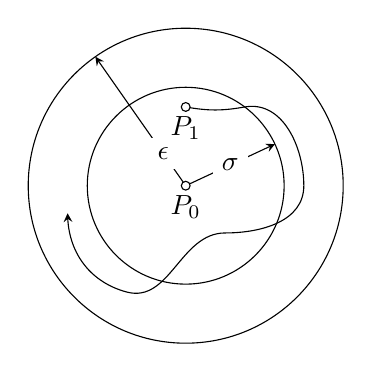
\begin{tikzpicture}
\draw(0,0) circle (1.25);
\draw(0,0) circle (2);
\draw[-stealth](0,0)--++(25:1.25)node[pos=0.5,fill=white]{$\sigma$};
\draw[-stealth](0,0)--++(125:2)node[pos=0.25,fill=white]{$\epsilon$};
\draw[fill=white](0,0) node [ocirc]{}node[below]{$P_0$};
%trajectory
\draw[-stealth](0,1)node[ocirc]{}node[below]{$P_1$} to [out=-10,in=-170]++(0.75,0) to [out=10,in=90]++(0.75,-1) to [out=-90,in=0]++(-1,-0.6) to [out=180,in=-15]++(-1.25,-.75) to [out=165,in=-90]++(-0.75,1);
\end{tikzpicture}
\caption*{(الف) مستحکم نقطہ فاصل \عددی{P_0} کی صورت میں خط حرکت \عددی{D_{\epsilon}} میں رہتی ہے۔}
\end{subfigure}%
\begin{subfigure}{0.5\textwidth}
\centering
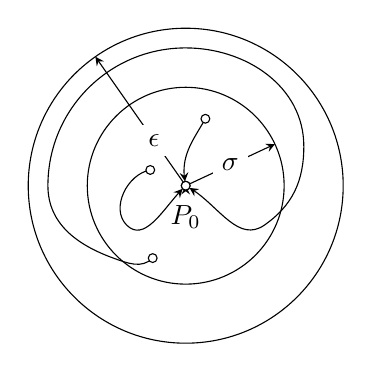
\begin{tikzpicture}
\draw(0,0) circle (1.25);
\draw(0,0) circle (2);
\draw[-stealth](0,0)--++(25:1.25)node[pos=0.5,fill=white]{$\sigma$};
\draw[-stealth](0,0)--++(125:2)node[pos=0.35,fill=white]{$\epsilon$};
\draw[fill=white](0,0) node [ocirc]{}node[shift={(0,-0.4)}]{$P_0$};
%trajectory
\draw[stealth-] (0,0)node[ocirc](ka){};\draw[stealth-] (ka) to [out=100,in=-120]++(0.25,0.85)node[ocirc]{};
\draw[stealth-](ka) to [out=-135,in=-45]++(-0.75,-0.5) to [out=135,in=-170]++(0.3,0.7)node[ocirc]{};
\draw[stealth-] (ka) to [out=-30,in=-145]++(1,-0.5) to [out=35,in=-90]++(0.5,1) to [out=90,in=0] (0,1.75) to [out=180,in=90] (-1.75,0) to [out=-90,in=160] (-135:1.3) to [out=-20,in=-135]++(0.5,0)node[ocirc]{};
\end{tikzpicture}
\caption*{(ب) مستحکم اور جاذب نقطہ فاصل \عددی{P_0}۔}
\end{subfigure}%
\caption{نظام \حوالہ{مساوات_نظام_جانچ_نقطہ_فاصل_الف} کے نقطہ فاصل۔}
\label{شکل_نظام_نقطہ_فاصل_تعریف}
\end{figure}%
%=====================

استحکام کی بنیاد پر نقطہ فاصل کی درجہ بندی جدول \حوالہ{جدول_نظام_نقطہ_فاصل_بالمقابل_استحکام} میں دی گئی ہے۔
\begin{table}
\caption{استحکام کی بنیاد پر نقطہ فاصل کی درجہ بندی۔}
\label{جدول_نظام_نقطہ_فاصل_بالمقابل_استحکام}
\centering
\begin{tabular}{rlr}
استحکام کی قسم& \عددی{p=\lambda_1+\lambda_2}& \عددی{q=\lambda_1\lambda_2}\\
\hline
(الف) مستحکم اور جاذب& \عددی{p<0} & \عددی{q>0}\\
(ب) مستحکم & \عددی{p\le 0} & \عددی{q>0}\\
(پ) غیر مستحکم & \multicolumn{2}{c}{ \عددی{p>0} \,\,\, یا \,\,\, \عددی{q<0}}
\end{tabular}
\end{table}
%===================

آئیں جدول \حوالہ{جدول_نظام_نقطہ_فاصل_اصول_جانچ} اور جدول \حوالہ{جدول_نظام_نقطہ_فاصل_بالمقابل_استحکام} کو حاصل کریں۔اگر \عددی{q=\lambda_1\lambda_2>0} ہو تب دونوں امتیازی اقدار مثبت ہوں گے یا دونوں امتیازی اقدار منفی ہوں گے اور یا امتیازی اقدار جوڑی دار مخلوط ہوں گے۔ اب اگر \عددی{p=\lambda_1+\lambda_2<0} ہو تب دونوں امتیازی اقدار  منفی ہوں گے یا (مخلوط جوڑی دار صورت میں) ان کا حقیقی جزو منفی ہو گا لہٰذا \عددی{P_0} مستحکم اور جاذب ہو گا۔ جدول \حوالہ{جدول_نظام_نقطہ_فاصل_بالمقابل_استحکام} کے بقایا دو نتائج کو آپ خود اسی طرح اخذ کر سکتے ہیں۔

 \عددی{\Delta <0} کی صورت میں امتیازی قدر جوڑی دار مخلوط \عددی{\lambda_1=\alpha+i\beta} اور \عددی{\lambda_2=\alpha-i\beta} ہوں گے۔ اب اگر \عددی{p=\lambda_1+\lambda_2=2\alpha<0} ہو تب مستحکم، جاذب نقطہ مرغولہ حاصل ہو گا۔اس کے برعکس \عددی{p=2\alpha>0} کی صورت میں غیر مستحکم نقطہ مرغولہ حاصل ہو گا۔

\عددی{p=0} کی صورت میں \عددی{\lambda_2=-\lambda_1} ہو گا اور یوں \عددی{q=\lambda_1\lambda_2=-\lambda_1^2} ہو گا۔اب اگر \عددی{q>0} ہو تب  \عددی{\lambda_1^2=-q<0} ہو گا لہٰذا \عددی{\lambda_1} اور \عددی{\lambda_2} خالص خیالی ہوں گے جن سے  \اصطلاح{دوری حل}\فرہنگ{حل!دوری}\حاشیہب{periodic solutions}\فرہنگ{solutions!periodic} حاصل ہو گا۔دوری حل کا خط حرکت ایسا بند دائرہ ہے جس کا وسط \عددی{P_0} ہے۔
%=================

\ابتدا{مثال}\شناخت{مثال_نظام_جدول_کا_استعمال}\quad جدول \حوالہ{جدول_نظام_نقطہ_فاصل_اصول_جانچ} اور جدول \حوالہ{جدول_نظام_نقطہ_فاصل_بالمقابل_استحکام} کا عملی استعمال\\
گزشتہ حصے کے مثال \حوالہ{مثال_نظام_غیر_متناسب_جوڑ} میں نظام \حوالہ{مساوات_نظام_خط_حرکت_الف} یعنی 
 \عددی{\bM{y}'=\begin{bmatrix} -2&1\\1&-2 \end{bmatrix} \bM{y}} کی بات کی گئی جہاں \عددی{p=-4}، \عددی{q=3} اور \عددی{\Delta=4} ہیں۔یوں جدول \حوالہ{جدول_نظام_نقطہ_فاصل_اصول_جانچ}-الف کے تحت نقطہ فاصل ایک جوڑ ہو گا۔جدول \حوالہ{جدول_نظام_نقطہ_فاصل_بالمقابل_استحکام}-الف کے تحت یہ جوڑ مستحکم اور جاذب ہے۔
\انتہا{مثال}
%=====================

\ابتدا{مثال}\شناخت{مثال_نظام_اسپرنگ_کمیت_نقطہ_فاصل}\quad اسپرنگ اور کمیت کی آزادانہ حرکت\\
اسپرنگ اور کمیت [حصہ \حوالہ{حصہ_سادہ_اسپرنگ_کمیت} دیکھیں] کے نظام \عددی{my''+cy'+ky=0} کا نقطہ فاصل دریافت کریں۔

حل:تفرقی مساوات کو معیاری صورت میں لکھنے کی خاطر \عددی{m} سے تقسیم کرتے  ہوئے \عددی{y''+\tfrac{c}{m}y'+\tfrac{k}{m}y=0} لکھتے ہیں۔دو رتبی مساوات سے تفرقی مساوات کا نظام حاصل کرنے کی خاطر [حصہ \حوالہ{حصہ_نظام_قالب} دیکھیں] ہم \عددی{y_1=y} اور \عددی{y_2=y'} لیتے ہیں۔یوں 
\عددی{y_2'=y''=-\tfrac{k}{m}y_1-\tfrac{c}{m}y_2} ہو گا۔اس طرح
\begin{align*}
\bM{y}'=\begin{bmatrix*}[r] 0&1\\-\frac{k}{m}&-\frac{c}{m}  \end{bmatrix*} \bM{y},\quad  \abs{\bM{A}-\lambda\bM{I}}=\begin{bmatrix} -\lambda&1\\-\frac{k}{m}&-\frac{c}{m}-\lambda \end{bmatrix}=\lambda^2+\frac{c}{m}\lambda+\frac{k}{m}=0
\end{align*}
لکھا جائے گا جس سے \عددی{p=-\tfrac{c}{m}}، \عددی{q=\tfrac{k}{m}} اور \عددی{\Delta=\tfrac{c^2}{m^2}-4\tfrac{k}{m}} ملتے ہیں جنہیں استعمال کرتے ہوئے جدول \حوالہ{جدول_نظام_نقطہ_فاصل_اصول_جانچ} اور جدول \حوالہ{جدول_نظام_نقطہ_فاصل_بالمقابل_استحکام} سے درج ذیل نتائج حاصل ہوتے ہیں جہاں \عددی{\Delta} اہم کردار ادا کرتا ہے۔
\begin{itemize}
\شے[بلا تقصیر] \عددی{c=0}، \عددی{p=0} اور \عددی{q>0}  وسط دیتا ہے۔
\شے[کم مقصور]  \عددی{c^2<4mk}، \عددی{p<0}، \عددی{q>0} اور \عددی{\Delta<0} مستحکم جاذب نقطہ مرغولہ دیتا ہے۔
\شے[فاصل تقصیر] \عددی{c^2=4mk}، \عددی{p<0}، \عددی{q>0} اور \عددی{\Delta=0}  مستحکم جاذب جوڑ دیتا ہے۔
\شے[زیادہ مقصور] \عددی{c^2>4mk}، \عددی{p<0}، \عددی{q>0} اور \عددی{\Delta>0} مستحکم جاذب جوڑ دیتا ہے۔
\end{itemize}
\انتہا{مثال}
%====================

\حصہء{سوالات}
سوال \حوالہ{سوال_نظام_نقطہ_فاصل_اور_حل_الف} تا سوال \حوالہ{سوال_نظام_نقطہ_فاصل_اور_حل_ب} کے نقطہ فاصل کی قسم جدول \حوالہ{جدول_نظام_نقطہ_فاصل_اصول_جانچ} اور جدول \حوالہ{جدول_نظام_نقطہ_فاصل_بالمقابل_استحکام} کی مدد سے  دریافت کریں۔ان کے حقیقی عمومی حل حاصل کریں اور ان کے خط حرکت کمپیوٹر کی مدد سے کھینچیں۔[پہلے چار جوابات کے خط حرکت دکھائے گئے ہیں۔]

%===========
\ابتدا{سوال}\شناخت{سوال_نظام_نقطہ_فاصل_اور_حل_الف}
\begin{align*}
y_1'&=y_1\\
y_2'&=3y_2
\end{align*}
جوابات:غیر مستحکم، غیر مناسب جوڑ۔\عددی{\bM{y}=c_1\begin{bmatrix} 1\\0  \end{bmatrix}e^t+c_2\begin{bmatrix} 0\\1 \end{bmatrix}e^{3t}} یعنی 
 \عددی{y_1=c_1e^t}، \عددی{y_2=c_2e^{3t}}؛ شکل \حوالہ{شکل_سوال_نظام_نقطہ_فاصل_اور_حل_الف}-الف۔
\begin{figure}
\centering
\begin{subfigure}{0.5\textwidth}
\centering
\begin{tikzpicture}
\begin{axis}[small,axis lines*=middle,xtick=\empty,ytick=\empty,xlabel={$y_1$},ylabel={$y_2$},xlabel style={at={(axis description cs:1.05,0.5)}},ylabel style ={rotate=-90},ylabel style={at={(axis description cs:0.5,1.05)}}]
\pgfmathsetmacro{\ca}{1}
\pgfmathsetmacro{\cb}{0}
\addplot[domain=0:3]({\ca*e^x},{\cb*e^(3*x)})node[pos=0.5](ka){}node[pos=0.501](kb){};
\draw[-stealth](ka)--(kb);
\pgfmathsetmacro{\ca}{-1}
\pgfmathsetmacro{\cb}{0}
\addplot[domain=0:3]({\ca*e^x},{\cb*e^(3*x)})node[pos=0.5](ka){}node[pos=0.501](kb){};
\draw[-stealth](ka)--(kb);
\pgfmathsetmacro{\ca}{0}
\pgfmathsetmacro{\cb}{1}
\addplot[domain=0:3]({\ca*e^x},{\cb*e^(3*x)})node[pos=0.5](ka){}node[pos=0.501](kb){};
\draw[-stealth](ka)--(kb);
\pgfmathsetmacro{\ca}{0}
\pgfmathsetmacro{\cb}{-1}
\addplot[domain=0:3]({\ca*e^x},{\cb*e^(3*x)})node[pos=0.5](ka){}node[pos=0.501](kb){};
\draw[-stealth](ka)--(kb);
%
\pgfmathsetmacro{\ca}{1}
\pgfmathsetmacro{\cb}{1}
\addplot[domain=0:3]({\ca*e^x},{\cb*e^(3*x)})node[pos=0.5](ka){}node[pos=0.501](kb){};
\draw[-stealth](ka)--(kb);
\pgfmathsetmacro{\ca}{1}
\pgfmathsetmacro{\cb}{-1}
\addplot[domain=0:3]({\ca*e^x},{\cb*e^(3*x)})node[pos=0.5](ka){}node[pos=0.501](kb){};
\draw[-stealth](ka)--(kb);
\pgfmathsetmacro{\ca}{-1}
\pgfmathsetmacro{\cb}{1}
\addplot[domain=0:3]({\ca*e^x},{\cb*e^(3*x)})node[pos=0.5](ka){}node[pos=0.501](kb){};
\draw[-stealth](ka)--(kb);
\pgfmathsetmacro{\ca}{-1}
\pgfmathsetmacro{\cb}{-1}
\addplot[domain=0:3]({\ca*e^x},{\cb*e^(3*x)})node[pos=0.5](ka){}node[pos=0.501](kb){};
\draw[-stealth](ka)--(kb);
\addplot[fill=white]plot coordinates {(0,0)}node[ocirc]{}; 
\end{axis}
\end{tikzpicture}
\caption*{(الف) سوال \حوالہ{سوال_نظام_نقطہ_فاصل_اور_حل_الف} غیر مستحکم، غیر مناسب جوڑ۔}
\end{subfigure}%
\begin{subfigure}{0.5\textwidth}
\centering
\begin{tikzpicture}
\begin{axis}[small,axis lines*=middle,xtick=\empty,ytick=\empty,xlabel={$y_1$},ylabel={$y_2$},xlabel style={at={(axis description cs:1.05,0.5)}},ylabel style ={rotate=-90},ylabel style={at={(axis description cs:0.5,1.05)}}]
\pgfmathsetmacro{\ca}{1}
\pgfmathsetmacro{\cb}{0}
\addplot[domain=0:3]({\ca*e^(-3*x)},{\cb*e^(-5*x)})node[pos=0.5](ka){}node[pos=0.501](kb){};
\draw[-stealth](ka)--(kb);
\pgfmathsetmacro{\ca}{-1}
\pgfmathsetmacro{\cb}{0}
\addplot[domain=0:3]({\ca*e^(-3*x)},{\cb*e^(-5*x)})node[pos=0.5](ka){}node[pos=0.501](kb){};
\draw[-stealth](ka)--(kb);
\pgfmathsetmacro{\ca}{0}
\pgfmathsetmacro{\cb}{1}
\addplot[domain=0:3]({\ca*e^(-3*x)},{\cb*e^(-5*x)})node[pos=0.5](ka){}node[pos=0.501](kb){};
\draw[-stealth](ka)--(kb);
\pgfmathsetmacro{\ca}{0}
\pgfmathsetmacro{\cb}{-1}
\addplot[domain=0:3]({\ca*e^(-3*x)},{\cb*e^(-5*x)})node[pos=0.5](ka){}node[pos=0.501](kb){};
\draw[-stealth](ka)--(kb);
%
\pgfmathsetmacro{\ca}{1}
\pgfmathsetmacro{\cb}{1}
\addplot[domain=0:3]({\ca*e^(-3*x)},{\cb*e^(-5*x)})node[pos=0.5](ka){}node[pos=0.501](kb){};
\draw[-stealth](ka)--(kb);
\pgfmathsetmacro{\ca}{1}
\pgfmathsetmacro{\cb}{-1}
\addplot[domain=0:3]({\ca*e^(-3*x)},{\cb*e^(-5*x)})node[pos=0.5](ka){}node[pos=0.501](kb){};
\draw[-stealth](ka)--(kb);
\pgfmathsetmacro{\ca}{-1}
\pgfmathsetmacro{\cb}{1}
\addplot[domain=0:3]({\ca*e^(-3*x)},{\cb*e^(-5*x)})node[pos=0.5](ka){}node[pos=0.501](kb){};
\draw[-stealth](ka)--(kb);
\pgfmathsetmacro{\ca}{-1}
\pgfmathsetmacro{\cb}{-1}
\addplot[domain=0:3]({\ca*e^(-3*x)},{\cb*e^(-5*x)})node[pos=0.5](ka){}node[pos=0.501](kb){};
\draw[-stealth](ka)--(kb);
\addplot[fill=white]plot coordinates {(0,0)}node[ocirc]{}; 
\end{axis}
\end{tikzpicture}
\caption*{(ب) سوال \حوالہ{سوال_نظام_نقطہ_فاصل_اور_حل_الف_ب}  مستحکم، جاذب، غیر مناسب جوڑ۔}
\end{subfigure}%
\caption{سوال \حوالہ{سوال_نظام_نقطہ_فاصل_اور_حل_الف} اور سوال \حوالہ{سوال_نظام_نقطہ_فاصل_اور_حل_الف_ب} کے اشکال۔}
\label{شکل_سوال_نظام_نقطہ_فاصل_اور_حل_الف}
\end{figure}
\انتہا{سوال}
%===========
\ابتدا{سوال}\شناخت{سوال_نظام_نقطہ_فاصل_اور_حل_الف_ب}
\begin{align*}
y_1'&=-3y_1\\
y_2'&=-5y_2
\end{align*}
جوابات:مستحکم، جاذب، غیر مناسب جوڑ۔  \عددیء{y_1=c_1e^{-3t}}، \عددی{y_2=c_2e^{-5t}}؛ شکل \حوالہ{شکل_سوال_نظام_نقطہ_فاصل_اور_حل_الف}-ب۔
\انتہا{سوال}
%=======================
\ابتدا{سوال}\شناخت{سوال_نظام_نقطہ_فاصل_اور_حل_الف_پ}
\begin{align*}
y_1'&=y_2\\
y_2'&=-16y_1
\end{align*}
جوابات:مستحکم وسط۔ \عددی{y_1=A\cos 4t+B\sin 4t}، \عددی{y_2=4B\cos 4t-4A\sin 4t}؛ شکل \حوالہ{شکل_سوال_نظام_نقطہ_فاصل_اور_حل_الف_پ}-الف۔
\begin{figure}
\centering
\begin{subfigure}{0.5\textwidth}
\centering
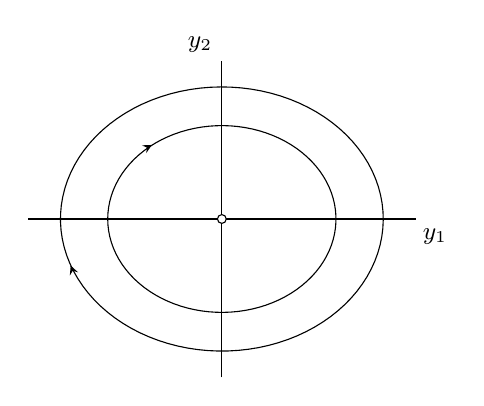
\begin{tikzpicture}
\begin{axis}[small,axis lines*=middle,xtick=\empty,ytick=\empty,xlabel={$y_1$},ylabel={$y_2$},xlabel style={at={(axis description cs:1.05,0.5)}},ylabel style ={rotate=-90},ylabel style={at={(axis description cs:0.5,1.05)}}]
\pgfmathsetmacro{\ca}{1}
\pgfmathsetmacro{\cb}{0}
\addplot[domain=-45:45,samples=100]({\ca*cos(4*x)+\cb*sin(4*x)},{4*\cb*cos(4*x)-4*\ca*sin(4*x)})node[pos=0.2](ka){}node[pos=0.201](kb){};
\draw[-stealth](ka)--(kb);
\pgfmathsetmacro{\ca}{1}
\pgfmathsetmacro{\cb}{1}
\addplot[domain=-45:45,samples=100]({\ca*cos(4*x)+\cb*sin(4*x)},{4*\cb*cos(4*x)-4*\ca*sin(4*x)})node[pos=0.1](ka){}node[pos=0.101](kb){};
\draw[-stealth](ka)--(kb);
%
\addplot[fill=white]plot coordinates {(0,0)}node[ocirc]{}; 
\end{axis}
\end{tikzpicture}
\caption*{(الف) سوال \حوالہ{سوال_نظام_نقطہ_فاصل_اور_حل_الف_پ}  مستحکم وسط۔}
\end{subfigure}%
\begin{subfigure}{0.5\textwidth}
\centering
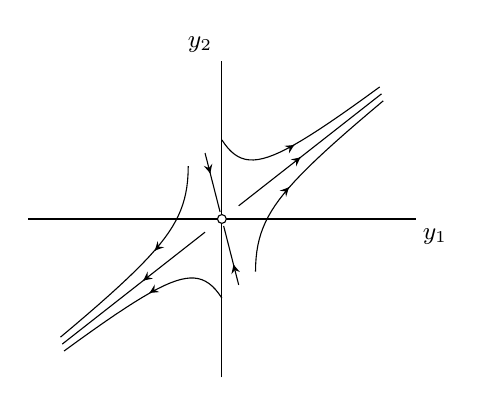
\begin{tikzpicture}
\begin{axis}[small,axis lines*=middle,xtick=\empty,ytick=\empty,xlabel={$y_1$},ylabel={$y_2$},xlabel style={at={(axis description cs:1.05,0.5)}},ylabel style ={rotate=-90},ylabel style={at={(axis description cs:0.5,1.05)}}]
\pgfmathsetmacro{\lmt}{0.75}
%
\pgfmathsetmacro{\ca}{1}
\pgfmathsetmacro{\cb}{1}
\addplot[domain=0:\lmt]({\ca*e^(-3*x)+\cb*e^(3*x)},{-5*\ca*e^(-3*x)+\cb*e^(3*x)})node[pos=0.5](ka){}node[pos=0.501](kb){};
\draw[-stealth](ka)--(kb);
\pgfmathsetmacro{\ca}{-1}
\pgfmathsetmacro{\cb}{1}
\addplot[domain=0:\lmt]({\ca*e^(-3*x)+\cb*e^(3*x)},{-5*\ca*e^(-3*x)+\cb*e^(3*x)})node[pos=0.5](ka){}node[pos=0.501](kb){};
\draw[-stealth](ka)--(kb);
\pgfmathsetmacro{\ca}{1}
\pgfmathsetmacro{\cb}{-1}
\addplot[domain=0:\lmt]({\ca*e^(-3*x)+\cb*e^(3*x)},{-5*\ca*e^(-3*x)+\cb*e^(3*x)})node[pos=0.5](ka){}node[pos=0.501](kb){};
\draw[-stealth](ka)--(kb);
\pgfmathsetmacro{\ca}{-1}
\pgfmathsetmacro{\cb}{-1}
\addplot[domain=0:\lmt]({\ca*e^(-3*x)+\cb*e^(3*x)},{-5*\ca*e^(-3*x)+\cb*e^(3*x)})node[pos=0.5](ka){}node[pos=0.501](kb){};
\draw[-stealth](ka)--(kb);
\pgfmathsetmacro{\ca}{0}
\pgfmathsetmacro{\cb}{1}
\addplot[domain=0:\lmt]({\ca*e^(-3*x)+\cb*e^(3*x)},{-5*\ca*e^(-3*x)+\cb*e^(3*x)})node[pos=0.5](ka){}node[pos=0.501](kb){};
\draw[-stealth](ka)--(kb);
\pgfmathsetmacro{\ca}{0}
\pgfmathsetmacro{\cb}{-1}
\addplot[domain=0:\lmt]({\ca*e^(-3*x)+\cb*e^(3*x)},{-5*\ca*e^(-3*x)+\cb*e^(3*x)})node[pos=0.5](ka){}node[pos=0.501](kb){};
\draw[-stealth](ka)--(kb);
\pgfmathsetmacro{\ca}{1}
\pgfmathsetmacro{\cb}{0}
\addplot[domain=0:\lmt]({\ca*e^(-3*x)+\cb*e^(3*x)},{-5*\ca*e^(-3*x)+\cb*e^(3*x)})node[pos=0.5](ka){}node[pos=0.51](kb){};
\draw[-stealth](ka)--(kb);
\pgfmathsetmacro{\ca}{-1}
\pgfmathsetmacro{\cb}{0}
\addplot[domain=0:\lmt]({\ca*e^(-3*x)+\cb*e^(3*x)},{-5*\ca*e^(-3*x)+\cb*e^(3*x)})node[pos=0.5](ka){}node[pos=0.51](kb){};
\draw[-stealth](ka)--(kb);
%
\addplot[fill=white]plot coordinates {(0,0)}node[ocirc]{}; 
\end{axis}
\end{tikzpicture}
\caption*{(ب) سوال \حوالہ{سوال_نظام_نقطہ_فاصل_اور_حل_الف_ت} غیر مستحکم، نقطہ زین۔}
\end{subfigure}%
\caption{سوال \حوالہ{سوال_نظام_نقطہ_فاصل_اور_حل_الف_پ} اور سوال \حوالہ{سوال_نظام_نقطہ_فاصل_اور_حل_الف_ت} کے اشکال۔}
\label{شکل_سوال_نظام_نقطہ_فاصل_اور_حل_الف_پ}
\end{figure}
\انتہا{سوال}
%========================
\ابتدا{سوال}\شناخت{سوال_نظام_نقطہ_فاصل_اور_حل_الف_ت}
\begin{align*}
y_1&=2y_1+y_2\\
y_2&=5y_1-2y_2
\end{align*}
جوابات: غیر مستحکم نقطہ زین؛ \عددی{y_1=c_1e^{-3t}+c_2e^{3t}}، \عددی{y_2=-5c_1e^{-3t}+c_2e^{3t}}؛شکل \حوالہ{شکل_سوال_نظام_نقطہ_فاصل_اور_حل_الف_پ}-ب۔
\انتہا{سوال}
%================
\ابتدا{سوال}\شناخت{سوال_نظام_نقطہ_فاصل_اور_حل_الف_ٹ}
\begin{align*}
y_1&=-2y_1-2y_2\\
y_2&=2y_1-2y_2
\end{align*}
جوابات:مستحکم اور جاذب نقطہ مرغولہ؛ \عددی{y_1=e^{-2t}(A\cos 2t+B\sin 2t)}، \عددی{y_2=e^{-2t}(-B\cos 2t+A\sin 2t)}
\انتہا{سوال}
%================
\ابتدا{سوال}
\begin{align*}
y_1&=-10y_1+2y_2\\
y_2&=-15y_1+y_2
\end{align*}
جوابات:مستحکم اور جاذب جوڑ؛ \عددی{y_1=c_1e^{-5t}+c_2e^{-4t}}، \عددی{y_2=\tfrac{5}{2}c_1e^{-5t}+3c_2e^{-4t}}
\انتہا{سوال}
%================
\ابتدا{سوال}
\begin{align*}
y_1&=-y_1+y_2\\
y_2&=2y_2
\end{align*}
جوابات:غیر مستحکم نقطہ زین؛ \عددی{y_1=c_1e^{-t}+c_2e^{2t}}، \عددی{y_2=3c_2e^{2t}}
\انتہا{سوال}
%================
\ابتدا{سوال}
\begin{align*}
y_1&=-y_1+2y_2\\
y_2&=6y_1+3y_2
\end{align*}
جوابات:غیر مستحکم نقطہ زین؛ \عددی{y_1=c_1e^{-3t}+c_2e^{5t}}، \عددی{y_2=-c_1e^{-3t}+3c_2e^{5t}}
\انتہا{سوال}
%================
\ابتدا{سوال}
\begin{align*}
y_1&=13y_1-3y_2\\
y_2&=18y_1-2y_2
\end{align*}
جوابات:غیر مستحکم جوڑ؛ \عددی{y_1=c_1e^{7t}+c_2e^{4t}}، \عددی{y_2=2c_1e^{7t}+3c_2e^{4t}}
\انتہا{سوال}
%================
\ابتدا{سوال}\شناخت{سوال_نظام_نقطہ_فاصل_اور_حل_ب}
\begin{align*}
y_1&=y_2\\
y_2&=-5y_1-2y_2
\end{align*}
جوابات:مستحکم اور جاذب نقطہ مرغولہ؛ \عددی{y_1=e^{-t}(A\cos 2t+B\sin 2t)}، \\ \عددی{y_2=e^{-t}[-(A+2B)\cos 2t-(2A+B)\sin 2t]}
\انتہا{سوال}
%================

سوال \حوالہ{سوال_نظام_نقطہ_فاصل_دو_درجی_الف} تا سوال \حوالہ{سوال_نظام_نقطہ_فاصل_دو_درجی_الف} خط حرکت، دو رتبی سادہ تفرقی مساوات اور نقطہ فاصل کے بارے میں ہیں۔

%==============
\ابتدا{سوال}\شناخت{سوال_نظام_نقطہ_فاصل_دو_درجی_الف} \quad قصری ارتعاش\\
\عددی{y''+4y'+5y=0} کو حل کریں۔امتیازی مساوات سے خط حرکت کی قسم دریافت کریں؟

جواب:\عددی{y=e^{-2t}(A\cos t+B\sin t)}؛ مستحکم اور جاذب نقطہ مرغولہ۔
\انتہا{سوال}
%====================
\ابتدا{سوال} \quad ہارمونی ارتعاش\\
\عددی{y''+4y=0=0} کو حل کریں۔امتیازی مساوات سے خط حرکت کی قسم دریافت کریں؟

جواب:\عددی{y=A\cos 2t+B\sin 2t}؛ مستحکم وسط۔
\انتہا{سوال}
%====================
\ابتدا{سوال} \quad مقدار معلوم کا تبادلہ\\
مثال \حوالہ{مثال_نظام_جدول_کا_استعمال} میں متغیرہ \عددی{\tau=-t} متعارف کرنے سے نقطہ فاصل پر کیا اثر پڑے گا؟

جواب: اب \عددی{\bM{A}=\begin{bmatrix*}[r] 2&-1\\-1&2  \end{bmatrix*}} ہو گا لہٰذا غیر مستحکم جوڑ پایا جائے گا۔
\انتہا{سوال}
%====================
\ابتدا{سوال} \quad وسط میں خلل\\
سوال \حوالہ{سوال_نظام_نقطہ_فاصل_اور_حل_الف_پ} میں \عددی{\bM{A}} کو تبدیل کرتے ہوئے \عددی{\bM{A}-0.12\bM{I}} کرنے سے نقطہ فاصل پر کیا اثر پیدا ہو گا؟ \عددی{\bM{I}}  اکائی قالب ہے۔ 

جواب: اب \عددی{p=-0.2=\ne 0}، \عددی{q >0} اور \عددی{\Delta <0} ہیں لہٰذا غیر مستحکم نقطہ مرغولہ پایا جائے گا۔
\انتہا{سوال}
%====================
\ابتدا{سوال} \quad وسط میں خلل\\
سوال \حوالہ{سوال_نظام_نقطہ_فاصل_اور_حل_الف_پ} میں تمام \عددی{a_{jk}} کی جگہ \عددی{a_{jk}+b} پر کریں۔ (الف) \عددی{b} کی ایسی قیمت دریافت کریں کہ نقطہ زین حاصل ہو۔اسی طرح \عددی{b} کی ایسی قیمتیں دریافت کریں جن پر (ب) مستحکم اور جاذب جوڑ، (پ) مستحکم اور جاذب نقطہ مرغولہ اور (ت) غیر مستحکم نقطہ مرغولہ پایا جائے۔

جواب:مثلاً (الف) \عددی{b=-2}، (ب) \عددی{b=-1}، (پ) \عددی{b=-0.2}، (ت) \عددی{b=15}
\انتہا{سوال}
%====================

\حصہ{کیفی تراکیب برائے غیر خطی نظام}
\اصطلاح{کیفی تراکیب}\فرہنگ{کیفی!تراکیب}\فرہنگ{ترکیب!کیفی}\حاشیہب{qualitative methods}\فرہنگ{qualitative methods} سے مسئلے کو حل کئے بغیر حل کے بارے میں کیفی معلومات حاصل کی جاتی ہیں۔ایسے مسائل جن کا \اصطلاح{تحلیلی حل} مشکل یا نا قابل حصول ہو، کے لئے یہ ترکیب خاص طور پر کار آمد ہے۔عملاً اہم کئی غیر خطی نظام
\begin{gather}\label{مساوات_نظام_غیر_خطی_ترکیب_مرحلہ_الف}
\begin{aligned}
\bM{y}'=\bM{f}(\bM{y})
\end{aligned}\quad \implies \quad 
\begin{aligned}
y_1&=f_1(y_1,y_2)\\
y_2&=f_2(y_1,y_2)
\end{aligned}
\end{gather}
کے لئے یہ درست ہے۔

گزشتہ حصے میں \اصطلاح{سطح مرحلہ کی ترکیب}\فرہنگ{سطح مرحلہ!ترکیب} خطی نظام کے لئے استعمال کیا گیا۔اس حصے میں اس ترکیب کو وسعت دے کر غیر خطی نظام کے لئے استعمال کیا جائے گا۔ ہم فرض کرتے ہیں کہ مساوات \حوالہ{مساوات_نظام_غیر_خطی_ترکیب_مرحلہ_الف} \اصطلاح{خود مختار}\فرہنگ{خود مختار}\حاشیہب{autonomous}\فرہنگ{autonomous} ہے یعنی اس میں غیر تابع متغیرہ \عددی{t} \ترچھا{صریحاً} نہیں پایا جاتا۔(اس حصے میں تمام مثال خود مختار ہیں۔) ہم یہاں بھی حل کی نسل پیش کریں گے۔اعدادی ترکیب سے ایک وقت میں صرف ایک (تقریباً درست) حل حاصل ہوتا ہے۔ اس لحاظ سے سطح مرحلہ کی ترکیب زیادہ مفید ثابت ہوتی ہے۔

گزشتہ حصے کے چند تصورات اس حصے میں بھی درکار ہیں۔ان میں \اصطلاح{سطح حرکت} (\عددیء{y_1 y_2} سطح)، \اصطلاح{خط حرکت} (مساوات \حوالہ{مساوات_نظام_غیر_خطی_ترکیب_مرحلہ_الف} کا \عددی{y_1 y_2} سطح پر حل)، مساوات \حوالہ{مساوات_نظام_غیر_خطی_ترکیب_مرحلہ_الف} کا \اصطلاح{پیکر مرحلہ} (تمام خط حرکت کا مجموعہ)،  اور مساوات \حوالہ{مساوات_نظام_غیر_خطی_ترکیب_مرحلہ_الف} کا \اصطلاح{نقطہ فاصل} (ایسا نقطہ \عددی{(y_1,y_2)} جہاں \عددیء{f_1(y_1,y_2)} اور \عددیء{f_2(y_1,y_2)} دونوں صفر کے برابر ہوں۔) کے تصورات شامل ہیں۔

مساوات \حوالہ{مساوات_نظام_غیر_خطی_ترکیب_مرحلہ_الف} کے کئی نقطہ فاصل ہو سکتے ہیں۔ ان پر باری باری بات کی جائے گی۔مبدا سے ہٹ کر پائے جانے والے نقطہ فاصل پر غور کرنے سے پہلے، تکنیکی آسانی کی خاطر، ایسے نقطہ فاصل کو گھمائے بغیر  مبدا پر منتقل کیا جائے گا۔مبدا \عددی{(0,0)} سے ہٹ کر پائے جانے والے نقطہ فاصل \عددی{P_0:(a,b)} کو گھمائے بغیر  مبدا \عددی{(0,0)} پر درج ذیل عمل سے منتقل کیا جاتا ہے۔
\begin{align*}
\tilde{y}_1=y_1-a,\quad \tilde{y}_2=y_2-b
\end{align*}
اس عمل کے بعد نقطہ فاصل \عددی{P_0} مبدا \عددی{(0,0)} پر پایا جائے گا۔یوں ہم فرض کر سکتے ہیں کہ یہاں دیے گئے تمام مثالوں میں نقطہ  فاصل کو مبدا پر منتقل کیا گیا ہے اور  \عددی{\tilde{y}_1}، \عددی{\tilde{y}_2} کی جگہ ہم \عددی{y_1} اور \عددی{y_2} ہی لکھیں گے۔ہم یہ بھی فرض کرتے ہیں کہ نقطہ فاصل  \اصطلاح{تنہا}\فرہنگ{تنہا}\حاشیہب{isolated}\فرہنگ{isolated} ہے یعنی ایسے کسی بھی کافی حد تک چھوٹی ٹکیا جس کا وسط مبدا پر پایا جاتا ہو میں مساوات  \حوالہ{مساوات_نظام_غیر_خطی_ترکیب_مرحلہ_الف} کا صرف  ایک عدد نقطہ فاصل پایا جاتا ہے۔ اگر مساوات \حوالہ{مساوات_نظام_غیر_خطی_ترکیب_مرحلہ_الف} کے محدود تعداد میں نقطہ فاصل پائے جاتے ہوں تب ایسے تمام نقطہ فاصل خود بخود تنہا ہوں گے۔
%=============

\جزوحصہء{غیر خطی نظام کو خطی بنانا}
عموماً نظام \حوالہ{مساوات_نظام_غیر_خطی_ترکیب_مرحلہ_الف} کو نقطہ فاصل \عددی{P_0:(0,0)} کے قریب خطی تصور کرتے ہوئے نظام کی \اصطلاح{استحکام} کی نوعیت دریافت کی جا سکتی ہے۔نظام \حوالہ{مساوات_نظام_غیر_خطی_ترکیب_مرحلہ_الف} کو \عددی{\bM{y}'=\bM{A}\bM{y}+\bM{h}(\bM{y})} لکھ کر \عددی{\bM{h}(\bM{y})} رد کرنے سے خطی نظام حاصل کیا جاتا ہے۔اس عمل کو تفصیلاً دیکھتے ہیں۔

ہم اگلے باب میں دیکھیں گے کہ عموماً تفاعل کو تسلسل \عددی{f(x)=c_0+c_1x+c_2x^2+c_3x^3+\cdots} کی صورت میں لکھا جا سکتا ہے۔اسی طرح ایک سے زیادہ متغیرات پر مبنی تفاعل کے تسلسل بھی لکھے جا سکتے ہیں۔آئیں ایسے ہی چند تفاعل مثلاً 
\begin{align*}
f_a(x)=2x^2+5x, \quad f_b(x,y)=2x^3-y^2+xy, \quad f_c(x,y)=2x^2-3y+5
\end{align*}
میں آزاد متغیرات صفر کے برابر پر کریں۔ ایسا کرنے سے \عددی{f_a(0)=0}، \عددی{f_b(0,0)=0} اور \عددی{f_c(0,0)=5} ملتا ہے۔آزاد متغیرات صفر کے برابر پر کرنے سے صرف اس تفاعل کی قیمت غیر صفر حاصل ہو گی جس میں \عددی{c_0} طرز کا بالکل علیحدہ مستقل پایا جاتا ہو جو متغیرات کے ساتھ ضرب نہ ہو۔

اب چونکہ \عددی{P_0} نقطہ فاصل ہے لہٰذا \عددی{f_1(0,0)=0}اور  \عددی{f_2(0,0)=0}  ہو گا۔اس کا مطلب ہے کہ ان تفاعل میں \عددی{c_0} طرز کا علیحدہ مستقل نہیں پایا جاتا لہٰذا ان کو درج ذیل لکھا جا سکتا ہے جہاں \عددی{h_1} اور \عددی{h_2} غیر خطی تفاعل ہیں۔
\begin{gather}\label{مساوات_نظام_غیر_خطی_ترکیب_مرحلہ_ب}
\begin{aligned}
\bM{y}'=\bM{A}\bM{y}+\bM{h}(\bM{y})
\end{aligned} \quad \implies \quad 
\begin{aligned}
y_1'&=a_{11}y_1+a_{12}y_2+h_1(y_1,y_2)\\
y_2'&=a_{21}y_1+a_{22}y_2+h_2(y_1,y_2)
\end{aligned}
\end{gather}
چونکہ نظام \حوالہ{مساوات_نظام_غیر_خطی_ترکیب_مرحلہ_الف} \اصطلاح{خود مختار} [جس میں \عددی{t} صریحاً نہیں پایا جاتا] تفاعل ہے لہٰذا \عددی{\bM{A}} مستقل مقدار ہو گا۔ اب \اصطلاح{خطی بنانے کا مسئلہ}\فرہنگ{مسئلہ خطی بنانا}\حاشیہب{linearization theorem}\فرہنگ{linearization theorem}\فرہنگ{theorem!linearization} پیش کرتے ہیں جس کا ثبوت اس کتاب میں پیش نہیں کیا جائے گا۔
%================================

\ابتدا{مسئلہ}\quad خطی بنانا\\
اگر نظام \حوالہ{مساوات_نظام_غیر_خطی_ترکیب_مرحلہ_الف} کے نقطہ فاصل \عددی{P_0:(0,0)} کی پڑوس میں  \عددی{f_1}، \عددی{f_2} اور ان کے جزوی تفرق استمراری ہوں، اور  مساوات \حوالہ{مساوات_نظام_غیر_خطی_ترکیب_مرحلہ_ب} میں مقطع \عددی{\bM{A}} غیر صفر \عددی{(\abs{\bM{A}} \ne \bM{0})} ہو تب نظام \حوالہ{مساوات_نظام_غیر_خطی_ترکیب_مرحلہ_الف} کے نقطہ فاصل کی قسم اور استحکام وہی ہوں گی جو درج ذیل \اصطلاح{خطی کردہ نظام}\فرہنگ{نظام!خطی کردہ}\حاشیہب{linearized system}\فرہنگ{system!linearized} کی ہوں گی
\begin{gather}\label{مساوات_نظام_غیر_خطی_ترکیب_مرحلہ_پ}
\begin{aligned}
\bM{y}'=\bM{A}\bM{y}
\end{aligned} \quad \implies \quad 
\begin{aligned}
y_1'&=a_{11}y_1+a_{12}y_2\\
y_2'&=a_{21}y_1+a_{22}y_2
\end{aligned}
\end{gather}
البتہ \عددیء{\bM{A}} کے خالص خیالی یا برابر امتیازی قدر ہونے کی صورت میں نظام \حوالہ{مساوات_نظام_غیر_خطی_ترکیب_مرحلہ_الف} کا نقطہ فاصل نظام \حوالہ{مساوات_نظام_غیر_خطی_ترکیب_مرحلہ_پ} کے نقطہ فاصل کی قسم کا ہو سکتا ہے یا وہ نقطہ مرغولہ ہو سکتا ہے۔ 
\انتہا{مسئلہ}
%=================

\ابتدا{مثال}\شناخت{مثال_نظام_دھاگے_سے_لٹکی_کمیت}\quad ہلکے ڈنڈے سے لٹکی کمیت کی آزادانہ ارتعاش۔ خطی بنانا\\
ہلکے ڈنڈے سے لٹکی کمیت کو شکل \حوالہ{شکل_مثال_نظام_دھاگے_سے_لٹکی_کمیت}-الف میں دکھایا گیا ہے۔ڈنڈے کی کمیت اور ہوا کی رکاوٹی قوت کو نظر انداز کرتے ہوئے نقطہ فاصل کا مقام اور اس کی نوعیت دریافت کریں۔
\begin{figure}
\centering
\begin{subfigure}{0.5\textwidth}
\centering
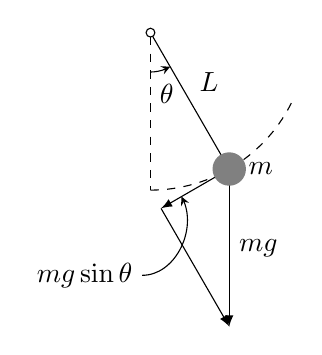
\begin{tikzpicture}
\pgfmathsetmacro{\ang}{60}
\pgfmathsetmacro{\lenL}{2}
\pgfmathsetmacro{\lenM}{2}
\pgfmathsetmacro{\lenA}{\lenM*cos(\ang)}
\pgfmathsetmacro{\lenB}{\lenM*sin(\ang)}
\pgfmathsetmacro{\lenH}{\lenM*cos(\ang)}
%vectors and lines
\draw[dashed]([shift={(-90:2)}]0,0) arc (-90:-25:2);
\draw[-latex] (-\ang:\lenL)--++(0,-\lenM)coordinate(kc)node[pos=0.5,right]{$mg$};
\draw[-latex](-\ang:\lenL)--++(-\ang-90:\lenH)coordinate(kd)coordinate[pos=0.7](ke);
\draw[-latex](kd)--(kc);
\draw[stealth-] (ke) to [out=-\ang,in=0]++(-0.5,-1)node[left]{$mg\sin \theta$};
%
\draw (0,0) node[ocirc](ka){}--++(-\ang:2)node[pos=0.5,above right]{$L$}node[circle,fill=gray,inner sep=1.5mm](kb){}node[shift={(0.4,0)}]{$m$};
\draw[dashed](ka)--++(-90:\lenM);
\draw[-stealth] ([shift={(-90:0.5)}]0,0) arc (-90:-\ang:0.5);
\draw (-75:0.8)node[]{$\theta$};
\end{tikzpicture}
\caption*{(الف) ہلکے ڈنڈے سے لٹکی کمیت کی آزادانہ ارتعاش۔}
\end{subfigure}%
\begin{subfigure}{0.5\textwidth}
\centering
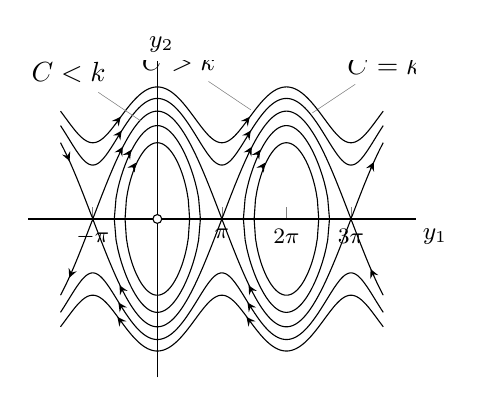
\begin{tikzpicture}
\begin{axis}[small,axis lines*=middle,xlabel={$y_1$},ylabel={$y_2$},xlabel style={at={(axis description cs:1.05,0.5)}},ylabel style={rotate=-90},ylabel style={at={(axis description cs:0.4,1.05)}},xtick={-180,180,360,540},xticklabels={$-\pi$,$\pi$,$2\pi$,$3\pi$},ytick=\empty]
\pgfmathsetmacro{\len}{2}
\pgfmathsetmacro{\k}{9.8/\len}   
%
\pgfmathsetmacro{\ca}{\k}   %  \ca=\k
\pgfmathsetmacro{\lmtS}{-180-90}
\pgfmathsetmacro{\lmtE}{\lmtS+900}    
\addplot[domain=\lmtS:\lmtE,samples=300]{sqrt(2*\k*cos(x)+2*\ca)}node[pos=0.04](ka){}node[pos=0.041](kb){}node[pos=0.2](kc){}node[pos=0.21](kd){}node[pos=0.6](ke){}node[pos=0.61](kf){}node[pos=0.975](kg){}node[pos=0.985](kh){}coordinate[pos=0.75](kkpin);
\draw(kkpin)node[pin=45:{$C=k$}]{};
\draw[-stealth] (ka)--(kb);
\draw[-stealth] (kc)--(kd);
\draw[-stealth] (ke)--(kf);
\draw[-stealth] (kg)--(kh);
\addplot[domain=\lmtS:\lmtE,samples=300]{-sqrt(2*\k*cos(x)+2*\ca)}node[pos=0.04](ka){}node[pos=0.041](kb){}node[pos=0.2](kc){}node[pos=0.21](kd){}node[pos=0.6](ke){}node[pos=0.61](kf){}node[pos=0.975](kg){}node[pos=0.985](kh){};
\draw[stealth-] (ka)--(kb);
\draw[stealth-] (kc)--(kd);
\draw[stealth-] (ke)--(kf);
\draw[stealth-] (kg)--(kh);
%
%
%
\pgfmathsetmacro{\ca}{1.5*\k}   %  \ca=1.5*\k
\pgfmathsetmacro{\lmtS}{-180-90}
\pgfmathsetmacro{\lmtE}{\lmtS+900}    
\addplot[domain=\lmtS:\lmtE,samples=300]{sqrt(2*\k*cos(x)+2*\ca)}node[pos=0.2](kc){}node[pos=0.21](kd){}node[pos=0.6](ke){}node[pos=0.61](kf){}coordinate[pos=0.62](kkpin);
\draw(kkpin)node[pin=135:{$C>k$}]{};
\draw[-stealth] (kc)--(kd);
\draw[-stealth] (ke)--(kf);
\addplot[domain=\lmtS:\lmtE,samples=300]{-sqrt(2*\k*cos(x)+2*\ca)}node[pos=0.2](kc){}node[pos=0.21](kd){}node[pos=0.6](ke){}node[pos=0.61](kf){};
\draw[stealth-] (kc)--(kd);
\draw[stealth-] (ke)--(kf);
%%
%
\pgfmathsetmacro{\ca}{2*\k}   %  \ca=2*\k
\pgfmathsetmacro{\lmtS}{-180-90}
\pgfmathsetmacro{\lmtE}{\lmtS+900}    
\addplot[domain=\lmtS:\lmtE,samples=300]{sqrt(2*\k*cos(x)+2*\ca)}node[pos=0.2](kc){}node[pos=0.21](kd){}node[pos=0.6](ke){}node[pos=0.61](kf){};
\draw[-stealth] (kc)--(kd);
\draw[-stealth] (ke)--(kf);
\addplot[domain=\lmtS:\lmtE,samples=300]{-sqrt(2*\k*cos(x)+2*\ca)}node[pos=0.2](kc){}node[pos=0.21](kd){}node[pos=0.6](ke){}node[pos=0.61](kf){};
\draw[stealth-] (kc)--(kd);
\draw[stealth-] (ke)--(kf);
%%%
\pgfmathsetmacro{\ca}{0.5*\k}   %  \ca=\k
\pgfmathsetmacro{\lmtS}{-120}
\pgfmathsetmacro{\lmtE}{\lmtS+240}    
\addplot[domain=\lmtS:\lmtE,samples=50]{sqrt(2*\k*cos(x)+2*\ca)}node[pos=0.25](ka){}node[pos=0.27](kb){}coordinate[pos=0.42](kkpin);
\draw(kkpin)node[pin=135:{$C<k$}]{};
\draw[-stealth] (ka)--(kb);
\addplot[domain=\lmtS:\lmtE,samples=50]{-sqrt(2*\k*cos(x)+2*\ca)};
%
\pgfmathsetmacro{\ca}{0.5*\k}   %  \ca=\k
\pgfmathsetmacro{\lmtS}{240}
\pgfmathsetmacro{\lmtE}{\lmtS+240}    
\addplot[domain=\lmtS:\lmtE,samples=50]{sqrt(2*\k*cos(x)+2*\ca)}node[pos=0.25](ka){}node[pos=0.27](kb){};
\draw[-stealth] (ka)--(kb);
\addplot[domain=\lmtS:\lmtE,samples=50]{-sqrt(2*\k*cos(x)+2*\ca)};
%%%
%%%
\pgfmathsetmacro{\ca}{0}   %  \ca=0
\pgfmathsetmacro{\lmtS}{-90}
\pgfmathsetmacro{\lmtE}{\lmtS+180}    
\addplot[domain=\lmtS:\lmtE,samples=50]{sqrt(2*\k*cos(x)+2*\ca)}node[pos=0.25](ka){}node[pos=0.27](kb){};
\draw[-stealth] (ka)--(kb);
\addplot[domain=\lmtS:\lmtE,samples=50]{-sqrt(2*\k*cos(x)+2*\ca)};
%
\pgfmathsetmacro{\ca}{0}   %  \ca=\k
\pgfmathsetmacro{\lmtS}{270}
\pgfmathsetmacro{\lmtE}{\lmtS+180}    
\addplot[domain=\lmtS:\lmtE,samples=50]{sqrt(2*\k*cos(x)+2*\ca)}node[pos=0.25](ka){}node[pos=0.27](kb){};
\draw[-stealth] (ka)--(kb);
\addplot[domain=\lmtS:\lmtE,samples=50]{-sqrt(2*\k*cos(x)+2*\ca)};
\addplot[fill=white] plot coordinates {(0,0)}node[ocirc]{};
\end{axis}
\end{tikzpicture}
\caption*{(ب) پیکر مرحلہ۔}
\end{subfigure}%
\caption{مثال \حوالہ{مثال_نظام_دھاگے_سے_لٹکی_کمیت} کے اشکال۔ [\عددی{C} کی تفصیل مثال \حوالہ{مثال_نظام_بلا_تقصیر_ارتعاش_یک_درجی_مساوات} میں دی جائے گی۔]}
\label{شکل_مثال_نظام_دھاگے_سے_لٹکی_کمیت}
\end{figure}
حل:\quad \موٹا{پہلا قدم} نمونہ کشی ہے۔متوازن مقام سے گھڑی کے الٹ رخ زاویائی فاصلہ \عددی{\theta} ناپتے ہیں۔قوت ثقل \عددی{mg} کمیت پر نیچے رخ عمل کرتا ہے جس کی وجہ سے حرکت کی مماسی، بحالی قوت \عددی{mg\sin \theta}  پیدا ہوتی ہے جہاں \عددی{g=\SI{.8}{\meter\per\second\squared}} ثقلی اسراع ہے۔\اصطلاح{نیوٹن}\فرہنگ{نیوٹن کا دوسرا قانون} کے دوسرے قانون کے تحت بحالی قوت اور اسراعی  قوت \عددی{mL\theta''} جہاں \عددی{L\theta''} اسراع ہے، ہر لمحہ برابر ہوں گے۔یوں ان دونوں قوتوں کا مجموعہ صفر کے برابر ہو گا۔
\begin{align*}
mL\theta''+mg\sin \theta=0
\end{align*}
دونوں اطراف کو \عددی{mL} سے تقسیم کرتے ہوئے
\begin{align}\label{مساوات_نظام_غیر_خطی_ترکیب_مرحلہ_ت}
\theta''+k\sin \theta=0,\quad \quad \left(k=\frac{g}{L}\right)
\end{align}
حاصل ہوتا ہے۔نہایت کم \عددی{\theta} کی صورت میں \عددی{\sin \theta \approx \theta} ہوتا ہے لہٰذا ایسی صورت میں درج بالا مساوات کو \عددی{\theta''+k\theta=0} لکھ کر حل \عددی{\theta=A\cos\sqrt{k}t+B\sin\sqrt{k} t} حاصل ہوتا ہے۔یہ کم \عددی{\theta} کی صورت میں تقریباً درست جواب ہے البتہ بالکل درست جواب \اصطلاح{بنیادی تفاعل}\فرہنگ{بنیادی تفاعل}\حاشیہب{elementary function}\فرہنگ{elementary function} کی صورت میں نہیں لکھا جا سکتا ہے۔

\موٹا{دوسرا قدم} \موٹا{نقطہ فاصل} \عددی{(0,0)}، \عددی{(\mp 2\pi,0)}، \عددی{(\mp 4\pi,0)}، \نقطے کا حصول  اور \موٹا{مسئلے کو خطی بنانا} ہے۔تفرقی مساوات کا نظام حاصل کرنے کی خاطر ہم \عددی{\theta=y_1} اور \عددی{\theta'=y_2} لکھتے ہیں۔ یوں مساوات \حوالہ{مساوات_نظام_غیر_خطی_ترکیب_مرحلہ_ت} سے درج ذیل نظام حاصل ہوتا ہے جو  نظام \حوالہ{مساوات_نظام_غیر_خطی_ترکیب_مرحلہ_الف} کے طرز کا ہے۔
\begin{gather}\label{مساوات_نظام_غیر_خطی_ترکیب_مرحلہ_ٹ}
\begin{aligned}
y_1'&=f_1(y_1,y_2)=y_2\\
y_2'&=f_2(y_1,y_2)=-k\sin y_1
\end{aligned}
\end{gather}
جہاں دونوں دائیں اطراف بیک وقت صفر کے برابر ہوں \عددی{y_2=0} اور \عددی{\sin y_1=0} وہاں نقطہ فاصل پایا جاتا ہے۔یوں لامحدود تعداد میں نقطہ فاصل \عددی{(n\pi,0)} پائے جاتے ہیں جہاں \عددی{n=0,\mp1,\mp2,\cdots} ہے۔آئیں نقطہ فاصل \عددی{(0,0)} پر غور کریں جہاں \اصطلاح{مکلارن تسلسل}\فرہنگ{مکلارن تسلسل}\فرہنگ{تسلسل!مکلارن}\حاشیہب{Maclaurin series}\فرہنگ{Maclaurin series} سے
\begin{align*}
\sin y_1=y_1-\frac{y_1^3}{6}+-\cdots \approx y_1
\end{align*}
لکھا جا سکتا ہے۔ یوں نقطہ فاصل کی پڑوس میں \عددی{h=-\tfrac{y_1^3}{6}+-\cdots} کو رد کرتے ہوئے  نظام \حوالہ{مساوات_نظام_غیر_خطی_ترکیب_مرحلہ_ٹ} کی خطی صورت
\begin{gather}
\begin{aligned}
y_1'&=y_2\\
y_2&=-ky_1
\end{aligned}\quad \implies \quad
\begin{aligned}
\bM{y}'=\bM{A} \bM{y}=\begin{bmatrix*}[r] 0&1\\-k&0 \end{bmatrix*}\bM{y}
\end{aligned}
\end{gather}
حاصل ہوتی ہے۔\عددی{p=a_{11}+a_{22}=0}، \عددی{q=\abs{\bM{A}}=k=\tfrac{g}{L} (> 0)} اور \عددی{\Delta=p^2-4q=-4k} لکھتے ہوئے نقطہ فاصل کی قسم اور اس کا استحکام جانتے ہیں ۔یوں جدول \حوالہ{جدول_نظام_نقطہ_فاصل_اصول_جانچ}-پ کے تحت \عددی{(0,0)} \اصطلاح{وسط} ہے اور جدول \حوالہ{جدول_نظام_نقطہ_فاصل_بالمقابل_استحکام} کے تحت یہ \اصطلاح{مستحکم}  ہے۔چونکہ \عددی{\sin y_1} دوری تفاعل ہے لہٰذا تمام \عددی{(n\pi,0)}، جہاں \عددی{n=\mp 2,\mp4,\cdots} ہے،  بھی مستحکم وسط ہیں۔ 
 
\موٹا{تیسرا قدم} \موٹا{نقطہ فاصل}  \عددی{(\mp \pi,0)}، \عددی{(\mp 3\pi,0)}، \عددی{(\mp 5\pi,0)} \نقطے کا حصول  اور \موٹا{مسئلے کو خطی بنانا} ہے۔ہم نقطہ فاصل \عددی{(\pi,0)} پر غور کرتے ہیں۔یوں \عددی{\theta-\pi=y_1} اور \عددی{(\theta-\pi)'=\theta'=y_2} لیتے اور مکلارن تسلسل
\begin{align*}
\sin(\theta)=\sin(y_1+\pi)=-\sin y_1=-y_1+\frac{y_1^3}{6}+-\cdots \approx -y_1
\end{align*}
کو استعمال کرتے ہوئے  نقطہ \عددی{(\pi,0)} پر نظام \حوالہ{مساوات_نظام_غیر_خطی_ترکیب_مرحلہ_ٹ} کی خطی کردہ صورت 
\begin{gather}
\begin{aligned}
y_1'&=y_2\\
y_2'&=ky_1
\end{aligned}\quad \implies \quad
\begin{aligned}
\bM{y}'=\bM{A}\bM{y}=\begin{bmatrix} 0&1\\ k&0 \end{bmatrix} \bM{y}
\end{aligned}
\end{gather}
حاصل ہوتی ہے۔اب \عددی{p=0}، \عددی{q=-k} اور \عددی{\Delta=-4q=4k} ہیں جو \اصطلاح{غیر مستحکم نقطہ زین} کو ظاہر کرتی ہے۔چونکہ \عددی{\sin y_1} دوری تفاعل ہے لہٰذا تمام \عددی{(n\pi,0)}،  جہاں \عددی{n=\mp1,\mp3,\cdots} ہے، غیر مستحکم نقطہ زین ہیں۔یہ نتائج شکل \حوالہ{شکل_مثال_نظام_دھاگے_سے_لٹکی_کمیت}-ب کے عین مطابق ہیں۔
\انتہا{مثال}
%=======================
\ابتدا{مثال}\شناخت{مثال_نظام_دھاگے_سے_لٹکی_کمیت_تقصیری}\quad ہلکے ڈنڈے سے لٹکی کمیت کی تقصیری ارتعاش۔ خطی بنانا\\
نقطہ فاصل پر غور کی ترکیب کو مزید بہتر جاننے کی خاطر مثال \حوالہ{مثال_نظام_دھاگے_سے_لٹکی_کمیت} میں زاویائی رفتار کے راست متناسب قوت روک \عددی{c\theta'} کا اثر شامل کرتے ہیں۔یوں مساوات \حوالہ{مساوات_نظام_غیر_خطی_ترکیب_مرحلہ_ت} درج ذیل صورت اختیار کرے گی جس میں \عددی{c=0} سے  مساوات \حوالہ{مساوات_نظام_غیر_خطی_ترکیب_مرحلہ_ت} ہی ملتا ہے۔
\begin{align}\label{مساوات_نظام_غیر_خطی_ترکیب_تقصیری_الف}
\theta''+c\theta'+k\sin \theta=0, \quad \quad (k>0), \quad (c\ge 0)
\end{align}
پہلے کی طرح \عددی{\theta=y_1} اور \عددی{\theta'=y_2} لکھتے ہوئے  غیر خطی نظام
\begin{align*}
y_1'&=y_2\\
y_2'&=-k\sin \theta-cy_2
\end{align*}
حاصل ہوتا ہے جہاں \عددی{\theta''=y_2'} لکھا گیا ہے۔اب بھی نقطہ فاصل \عددی{(0,0)}، \عددی{(\mp \pi,0)}، \عددی{\mp 2\pi,0}، \نقطے  پر پائے جاتے ہیں۔آئیں نقطہ \عددی{(0,0)} پر غور کریں۔یہاں بھی \عددی{\sin y_1 \approx y_1} لکھ کر \عددی{(0,0)} پر خطی نظام
\begin{gather}
\begin{aligned}
y_1'&=y_2\\
y_2'&=-ky_1 -cy_2
\end{aligned}\quad \implies \quad
\begin{aligned}
\bM{y}=\bM{A}\bM{y}=\begin{bmatrix*}[r] 0&1\\-k&-c \end{bmatrix*}\bM{y}
\end{aligned}
\end{gather}
 حاصل کرتے ہیں۔ یہ بالکل مثال \حوالہ{مثال_نظام_اسپرنگ_کمیت_نقطہ_فاصل} کی طرح ہے ماسوائے (مثبت) \عددی{m} کی موجودگی کے  (اور  ماسوائے \عددی{y_1} کے مطلب میں فرق کے)۔ اس طرح بلا تقصیر \عددی{(c=0)} صورت میں \اصطلاح{وسط} حاصل ہوتا ہے جسے شکل \حوالہ{شکل_مثال_نظام_دھاگے_سے_لٹکی_کمیت} میں دکھایا گیا ہے جبکہ کم تقصیری صورت میں \اصطلاح{نقطہ مرغولہ} حاصل ہوتا ہے ، اور اسی طرح آپ تمام صورتیں حاصل کر سکتے ہیں۔

آئیں اب نقطہ فاصل \عددی{(\pi,0)} پر غور کریں۔یوں \عددی{\theta-\pi=y_1} اور \عددی{(\theta-\pi)'=\theta'=y_2} کے علاوہ 
\begin{align*}
\sin \theta=\sin(y_1+\pi)=-\sin y_1\approx -y_1
\end{align*}
لکھ کر \عددی{(\pi,0)} پر خطی نظام
\begin{gather}
\begin{aligned}
y_1'&=y_2\\
y_2'&=ky_1-cy_2
\end{aligned}\quad \implies \quad
\begin{aligned}
\bM{y}'=\bM{A}\bM{y}=\begin{bmatrix*}[r] 0&1\\k&-c  \end{bmatrix*} \bM{y}
\end{aligned}
\end{gather}
حاصل کرتے ہیں۔گزشتہ حصے میں نقطہ فاصل کے جانچ کے مسلمہ معیار دیے گئے جن کے لئے 
\begin{align*}
p=a_{11}+a_{22}=-c, \quad q=\abs{\bM{A}}=-k, \quad \Delta=p^4-4q=c^2+4k
\end{align*}
حاصل کرتے ہیں۔ یوں \عددی{(\pi,0)} پر پائے جانے والے نقطہ فاصل کے لئے درج ذیل حاصل ہوتا ہے۔
\begin{itemize}
\شے{بلا تقصیر} \عددی{c=0}، \عددی{p=0}، \عددی{q<0} اور \عددی{\Delta >0}  نقطہ زین دیگا۔[شکل \حوالہ{شکل_مثال_نظام_دھاگے_سے_لٹکی_کمیت}-ب دیکھیں۔]
\شے{تقصیری} \عددی{c>0}، \عددی{p<0}، \عددی{q<0} اور \عددی{\Delta>0} نقطہ زین دیگا۔
\end{itemize}
چونکہ \عددی{\sin y_1} دوری عرصہ \عددی{2\pi} کا دوری تفاعل ہے  لہٰذا \عددی{(\mp 2\pi,0)}، \عددی{(\mp 4\pi,0)}، \نقطے پر اسی قسم کا نقطہ فاصل پایا جائے گا جو \عددی{(0,0)} پر پایا جاتا ہے اور اسی طرح \عددی{(-\pi,0)}، \عددی{(\mp 3\pi,0)}، \نقطے پر اسی قسم کا نقطہ فاصل پایا جائے گا جو \عددی{(\pi,0)} پر پایا جاتا ہے۔ 
\begin{figure}
\centering
\includegraphics{figSystemPendulumLossyA}
\caption{تقصیری ارتعاش۔مثال \حوالہ{مثال_نظام_دھاگے_سے_لٹکی_کمیت_تقصیری}}
\label{شکل_مثال_نظام_دھاگے_سے_لٹکی_کمیت_تقصیری}
\end{figure}

شکل \حوالہ{شکل_مثال_نظام_دھاگے_سے_لٹکی_کمیت_تقصیری} میں نظام \حوالہ{مساوات_نظام_غیر_خطی_ترکیب_تقصیری_الف} کے خط حرکت دکھائے گئے ہیں۔چونکہ قصری نظام میں توانائی کا ضیاع پایا جاتا ہے لہٰذا شکل \حوالہ{شکل_مثال_نظام_دھاگے_سے_لٹکی_کمیت} کے بند دائروں کی بجائے شکل \حوالہ{شکل_مثال_نظام_دھاگے_سے_لٹکی_کمیت_تقصیری} کے مرغولی خطوط حاصل ہوتے ہیں جو ہمارے توقع کے عین مطابق ہے۔مزید یہ کہ دوری لہری خطوط بھی کسی نہ کسی مقام پر نقطہ فاصل کے گرد گھومنا شروع کر دیتے ہیں۔ اس کے علاوہ اب قصری نظام میں نقطہ زین کو ملانے والے خط نہیں پائے جاتے۔
\انتہا{مثال}
%======================
\ابتدا{مثال}\شناخت{مثال_نظام_شکار_شکاری}\quad آبادی شکار اور شکاری۔ [مسئلہ لوٹکا-ولٹیرا]\\
یہاں لومڑی (شکاری) اور خرگوش (شکار) کی آبادی کے مسئلے پر غور کرتے ہیں۔

\موٹا{پہلا قدم}: ہم فرض کرتے ہیں کہ خرگوش کو جتنی خوراک چاہیے دستیاب ہے۔ یوں لومڑی کی غیر موجودگی میں ان کی تعداد \عددی{y_1'=ay_1} کے تحت قوت نمائی طور پر بڑھے گی۔ لومڑی کی موجودگی میں (اتفاقی آمنے سامنے سے)  خرگوش کی تعداد میں \عددی{y_1y_2} کے راست متناسب کمی پیدا ہو گی۔یوں خرگوش کی تعداد \عددی{y_1'=ay_1-by_1y_2} سے حاصل ہو گی جہاں مستقل \عددی{a>0} اور \عددی{b>0} ہیں۔اسی طرح خرگوش کی غیر موجودگی میں لومڑی کی تعداد \عددی{y_2'=-ly_2} کے تحت قوت نمائی طور پر گھٹے گی۔خرگوش کی موجودگی میں (اتفاقی آمنے سامنے سے) لومڑی کی تعداد \عددی{y_1y_2} کے راست متناسب بڑھے گی۔یوں خرگوش کی موجودگی میں  \عددی{y_2'=-ly_2+ky_1y_2} لومڑی کی تعداد دے گا جہاں مستقل \عددی{l>0} اور \عددی{k>0} ہیں۔

یوں غیر خطی \اصطلاح{مسئلہ لوٹکا-ولٹیرا}\حاشیہد{امریکی ماہر حیاتی طبیعیات الفرڈ جیمز لوٹکا [1880-1949] اور اطالوی ریاضی دان ویٹو ولٹیرا [1860-1940] نے شکار اور شکاری کے مسئلے کو پیش کیا۔} 
\begin{gather}\label{مثال_نظام_شکار_شکاری_الف}
\begin{aligned}
y_1'&=f_1(y_1,y_2)=ay_1-by_1y_2\\
y_2'&=f_2(y_1,y_2)=ky_1y_2-ly_2
\end{aligned}
\end{gather}
حاصل ہوتا ہے۔

\موٹا{دوسرا قدم} مسئلے کو خطی بنانا اور نقطہ فاصل \عددی{(0,0)} کا حصول  ہے۔مساوات \حوالہ{مثال_نظام_شکار_شکاری_الف} کو دیکھ کر نقطہ فاصل مساوات 
\begin{align}
f_1(y_1,y_2)=y_1(a-by_2)=0, \quad f_2(y_1,y_2)=y_2(ky_1-l)=0
\end{align}
کے حل سے \عددی{(y_1,y_2)=(0,0)} اور \عددی{(\tfrac{l}{k},\tfrac{a}{b})} حاصل ہوتے ہیں۔آئیں \عددی{(0,0)} پر غور کریں۔ نقطہ \عددی{(0,0)} کی پڑوس میں مساوات \حوالہ{مثال_نظام_شکار_شکاری_الف} میں \عددی{-by_1y_2} اور \عددی{ky_1y_2} کو نظر انداز کرتے ہوئے خطی نظام
\begin{align*}
\bM{y}'=\begin{bmatrix*}[r] a&0\\0&-l \end{bmatrix*}\bM{y}
\end{align*}
حاصل ہوتا ہے جس کی امتیازی اقدار \عددی{\lambda_1=a>0} اور \عددی{\lambda_2=-l<0} کی علامتیں آپس میں الٹ ہیں لہٰذا \عددی{(0,0)} پر نقطہ زین پایا جاتا ہے۔

\موٹا{تیسرا قدم} مسئلے کو خطی بنانا اور نقطہ فاصل \عددی{(\tfrac{l}{k},\tfrac{a}{b})} کا حصول  ہے۔دوسرا نقطہ فاصل \عددی{(y_1,y_2)=(\tfrac{l}{k},\tfrac{a}{b})} پر پایا جاتا ہے۔اس نقطے  کو \عددی{(0,0)} منتقل کرنے کی خاطر ہم \عددی{y_1=\tilde{y}_1+\tfrac{l}{k}} اور \عددی{y_2=\tilde{y}_2+\tfrac{a}{b}} چنتے ہیں۔یوں نقطہ فاصل \عددی{(\tilde{y}_1,\tilde{y}_2)=(0,0)} لکھا جا سکتا ہے۔ چونکہ \عددی{y_1=\tilde{y}_1'} اور \عددی{y_2'=\tilde{y}_2'} ہیں لہٰذا نظام \حوالہ{مثال_نظام_شکار_شکاری_الف} کو درج ذیل لکھا جا سکتا ہے۔
\begin{align*}
\tilde{y}_1'&=\left(\tilde{y}_1+\frac{l}{k}\right)\left[a-b\left(\tilde{y}_2+\frac{a}{b}\right)\right]=\left(\tilde{y}_1+\frac{l}{k}\right)(-b\tilde{y}_2)\\
\tilde{y}_2'&=\left(\tilde{y}_2+\frac{a}{b}\right)\left[k\left(\tilde{y}_1+\frac{l}{k}\right)-l\right]=\left(\tilde{y}_2+\frac{a}{b}\right)k\tilde{y}_1
\end{align*}
نقطہ \عددی{(\tilde{y}_1,\tilde{y}_2)=(0,0)} کی پڑوس میں \عددی{-b\tilde{y}_1\tilde{y}_2} اور \عددی{k\tilde{y}_1\tilde{y}_2} کو نظر انداز کرتے ہوئے خطی نظام
\begin{gather}\label{مثال_نظام_شکار_شکاری_ب}
\begin{aligned}
\tilde{y}_1'&=-\frac{bl}{k}\tilde{y}_2\quad \quad \text{(الف)}\\
\tilde{y}_2'&=\frac{ak}{b}\tilde{y}_1\quad \quad \text{(ب)}
\end{aligned}
\end{gather}
حاصل ہوتا ہے۔مساوات \حوالہ{مثال_نظام_شکار_شکاری_ب}-الف کا بایاں ہاتھ ضرب مساوات-ب کا دایاں ہاتھ برابر ہو گا الف کا دایاں ضرب ب کا بایاں،
\begin{align*}
\frac{ak}{b}\tilde{y}_1'\tilde{y}_1=-\frac{bl}{k}\tilde{y}_2'\tilde{y}_2 \implies \frac{ak}{b}\tilde{y}_1^2+\frac{bl}{k}\tilde{y}_2^2=C
\end{align*}
جس کا تکمل لیتے ہوئے \عددی{\tilde{y}_1} بالمقابل \عددی{\tilde{y}_2} کا \اصطلاح{ترخیمی}\فرہنگ{ترخیم}\حاشیہب{elliptic}\فرہنگ{elliptic} تعلق حاصل کیا گیا ہے۔یوں \عددی{(\tfrac{l}{k},\tfrac{a}{b})} پر شکل \حوالہ{شکل_مثال_نظام_شکار_شکاری} میں دکھایا گیا \اصطلاح{وسط} پایا جاتا ہے۔
\begin{figure}
\centering
\begin{tikzpicture}
%axis
\draw(0,0)--++(4,0)node[right]{$y_1$};
\draw(0,0)--++(0,2)node[left]{$y_2$};
\draw[->-=0.25] ([shift={(0:1cm and 0.5cm)}]2,1) arc  (0:180:1cm and 0.5cm) arc (-180:0:1cm and 0.5cm);
\draw[fill=white](2,1) node[ocirc](kc){};
\draw[dashed] (kc)--(0,1)node[left]{$\frac{a}{b}$};
\draw[dashed](kc)--(2,0)node[below]{$\frac{l}{k}$};
\end{tikzpicture}
\caption{شکار اور شکاری کی آبادی: ماحولیاتی توازن۔}
\label{شکل_مثال_نظام_شکار_شکاری}
\end{figure}

نسبتاً مشکل تجزیے سے ثابت کیا جا سکتا ہے کہ غیر خطی نظام \حوالہ{مثال_نظام_شکار_شکاری_الف} کا \عددی{(\tfrac{l}{k},\tfrac{a}{b})}  پر وسط پایا جاتا ہے البتہ خط حرکت اس نقطے کے گرد غیر ترخیمی بند دائرہ بناتا ہے۔

شکل \حوالہ{شکل_مثال_نظام_شکار_شکاری} کے دائیں کنارے پر خرگوش کی تعداد \عددی{y_1} زیادہ سے زیادہ ہے جس کی وجہ سے لومٹری کی تعداد \عددی{y_2} میں اضافے کی شرح بھی زیادہ سے زیادہ ہے۔اس خط پر گھڑی کی الٹی سمت چلتے ہوئے لومڑی کی زیادہ سے زیادہ آبادی حاصل ہوتی ہے۔اس مقام پر خرگوش کی تعداد اتنی کم ہو چکی ہوتی ہے کہ لومڑی کی بڑھتی تعداد کو خوراک پورا نہیں ہو پایا لہٰذا لومڑی کی آبادی گھٹنے شروع ہو جاتی ہے۔آپ دیکھ سکتے ہیں کہ دونوں جانوروں کی دوری تعداد حالات کے مطابق مسلسل تبدیل ہوتی ہے۔

شکار اور شکاری کی دیگر مثالیں ملخ اور گھاس، ببر شیر اور زیبرا ہیں۔
\انتہا{مثال}
%=====================


\جزوحصہ{سطح حرکت پر یک رتبی مساوات میں تبادلہ}
سطح حرکت کی دوسری ترکیب خود مختار [جس میں \عددیء{t} صریحاً نہیں پایا جاتا] دو رتبی سادہ تفرقی مساوات
\begin{align*}
F(y,y',y'')=0
\end{align*}
میں \عددی{y=y_1} کو آزاد متغیرہ اور \عددی{y'=y_2} لے کر \عددی{y''} کو زنجیری تفرق سے
\begin{align*}
y''=y_2'=\frac{\dif y_2}{\dif t}=\frac{\dif y_2}{\dif y_1}\frac{\dif y_1}{\dif t}=\frac{\dif y_2}{\dif y_1}y_2
\end{align*}
لکھ کر یک رتبی مساوات
\begin{align}
F\left(y_1,y_2,\frac{\dif y_2}{\dif y_1}y_2\right)=0
\end{align}
میں تبدیل کرنے پر مبنی ہے۔اس یک رتبی مساوات کو یا تو حل کرنا ممکن ہوتا ہے اور یا \اصطلاح{میدان ڈھال}\فرہنگ{میدان!ڈھال}\فرہنگ{ڈھال!میدان} کی مدد سے اس پر غور ممکن ہوتا ہے۔ آئیں مثال \حوالہ{مثال_نظام_دھاگے_سے_لٹکی_کمیت} پر اس ترکیب کی مدد سے غور کریں۔
%==========

\ابتدا{مثال}\شناخت{مثال_نظام_بلا_تقصیر_ارتعاش_یک_درجی_مساوات}\quad بلا تقصیر ارتعاشی نظام کی یک رتبی تفرقی مساوات۔\\
مساوات \حوالہ{مساوات_نظام_غیر_خطی_ترکیب_مرحلہ_ت} میں \عددی{\theta''+k\sin \theta=0} ہے جس میں \عددی{\theta=y_1} اور  \عددی{\theta'=y_2} (زاویائی رفتار) لیتے ہوئے
\begin{align*}
\theta''=\frac{\dif y_2}{\dif t}=\frac{\dif y_2}{\dif y_1}\frac{\dif y_1}{\dif t}=\frac{\dif y_2}{\dif y_1}y_2
\end{align*}
لکھ کر \عددی{\tfrac{\dif y_2}{\dif y_1}y_2=-k\sin y_1} ملتا ہے جس کو علیحدگی متغیرات سے \عددی{y_2\dif y_2=-k\sin y_1\dif y_1} لکھا جا سکتا ہے جس کا تکمل
\begin{align}\label{مساوات_نظام_کل_توانائی_الف}
\frac{1}{2}y_2^2=k\cos y_1+C 
\end{align}
دیتا ہے جہاں \عددی{C} تکمل کا مستقل ہے۔اس کو \عددی{mL^2} سے ضرب دینے سے
\begin{align*}
\frac{1}{2}m(Ly_2)^2-mL^2k\cos y_1=mL^2C
\end{align*}
حاصل ہوتا ہے جس کے تینوں اجزاء \اصطلاح{توانائی}\فرہنگ{توانائی}\حاشیہب{energy}\فرہنگ{energy} کو ظاہر کرتے ہیں۔چونکہ \عددی{y_2} زاویائی رفتار ہے لہٰذا \عددی{Ly_2} لمحاتی رفتار اور  \عددی{\tfrac{1}{2}m(Ly_2)^2} \اصطلاح{حرکی توانائی}\فرہنگ{حرکی توانائی}\فرہنگ{توانائی!حرکی}\حاشیہب{kinetic energy}\فرہنگ{energy!kinetic} ہے۔درج بالا مساوات کا دوسرا جزو (بمع منفی علامت) \اصطلاح{مخفی توانائی}\فرہنگ{توانائی!مخفی}\فرہنگ{مخفی توانائی}\حاشیہب{potential energy}\فرہنگ{energy!potential} ہے جبکہ مساوات کا دایاں ہاتھ \عددی{mL^2C} کل توانائی ہے۔بلا تقصیر نظام میں توانائی کا ضیاع نہیں پایا جاتا لہٰذا حزب توقع کل توانائی مستقل مقدار ہے۔آئیں دیکھیں کہ حرکت کی نوعیت کل توانائی پر کیسے منحصر ہے۔

شکل \حوالہ{شکل_مثال_نظام_دھاگے_سے_لٹکی_کمیت}-ب مختلف \عددی{C} کے لئے خط حرکت دیتی ہے۔ان خطوط کا دوری عرصہ \عددی{2\pi} ہے۔ان میں ترخیمی بند دائرے اور  لہر نما خطوط شامل ہیں جن کے مابین نقطہ زین [\عددی{(n\pi,0)} جہاں \عددی{n=\mp1,\mp3,\cdots} ہے] سے گزرتے ہوئے دو عدد خط حرکت  پائے جاتے ہیں۔مساوات \حوالہ{مساوات_نظام_کل_توانائی_الف} کے تحت \عددی{C} کی کم سے کم قیمت \عددی{C=-k} ہے جس پر \عددی{y_2=0} اور \عددی{\cos y_1=1} ہوں گے جو ساکن کمیت کو ظاہر کرتی ہے۔جس نقطے پر \عددی{y_2=\theta'=0} ہو اس نقطے پر حرت کی سمت تبدیل ہو کر الٹ ہو جائے گی لہٰذا مساوات \حوالہ{مساوات_نظام_کل_توانائی_الف} میں \عددی{y_2=0} پر کرتے ہوئے \عددی{k\cos y_1+C=0} حاصل ہوتا ہے۔اب اگر \عددی{y_1=\pi} ہو تب \عددی{\cos y_1=-1} اور یوں \عددی{C=k} ہو گا۔اس طرح اگر \عددی{-k<C<k} ہو تب \عددی{\abs{y_1}=\abs{\theta}<\pi} کی صورت میں کمیت کی حرکت کی سمت الٹ ہو گی اور \عددی{C} کی ان قیمتوں \عددی{(\abs{C}<k)} کے لئے کمیت ارتیاش پذیر ہو گا۔ترخیمی بند دائرے اس ارتعاشی حرکت کو ظاہر کرتے ہیں۔اس کے برعکس \عددی{C>k} کی صورت میں \عددی{y_2=0} ممکن نہیں ہے لہٰذا کمیت کی حرکت کی سمت الٹ نہیں ہو گی لہٰذا کمیت مبدا  کے گرد گھومتا رہے گا جس کو لہری خط حرکت ظاہر کرتی ہیں۔ان دو صورتوں کے مابین \عددی{C=k} پایا جاتا ہے جس کے خطوط نقطہ زین  سے گزرتے ہیں۔انہیں شکل \حوالہ{شکل_مثال_نظام_دھاگے_سے_لٹکی_کمیت}-ب  میں دکھایا گیا ہے۔
\انتہا{مثال}
%=================== 

دو رتبی مساوات کے تبادلے سے سطح حرکت پر (مثال \حوالہ{مثال_نظام_بلا_تقصیر_ارتعاش_یک_درجی_مساوات} کی طرح) قابل حل یک رتبی مساوات کے علاوہ نا قابل حل مساوات بھی اہمیت کے حامل ہے۔ایسی صورت میں میدان ڈھال [حصہ \حوالہ{حصہ_سادہ_ایک_درجی_ڈھال} دیکھیں۔] کے ذریعہ نظام کے بارے میں معلومات حاصل کرنا ممکن ہوتا ہے۔اس عمل کو ایک مشہور مثال کی مدد سے دیکھتے ہیں۔

%===============
\ابتدا{مثال}\quad منحصر بہ خود ارتعاش۔ مساوات ون در پول\\
ایسی طبعی نظام پائے جاتے ہیں جن میں معمولی ارتعاش کی صورت میں نظام کو توانائی فراہم ہوتی ہے جبکہ وسیع ارتعاش کی صورت میں نظام سے توانائی کا اخراج ہوتا ہے۔یوں وسیع ارتعاش کی صورت میں نظام قصری صورت اختیار کرتا ہے جبکہ کم ارتعاش کی صورت میں نظام میں \ترچھا{منفی تقصیر} (نظام کو توانائی کی فراہمی) پائی جاتی ہے۔ ہم طبعی وجوہات کی بنا توقع کرتے ہیں کہ ایسا نظام دوری طرز عمل رکھے گا، جو سطح حرکت پر بند دائرے کی صورت اختیار کرے گا جسے  \اصطلاح{تحدیدی دائرہ}\فرہنگ{تحدیدی دائرہ}\حاشیہب{limit cycle}\فرہنگ{limit cycle} کہتے ہیں۔ایسی ارتعاش کو \اصطلاح{مساوات ون در پول}\فرہنگ{مساوات!ون در پول}\فرہنگ{ون در پول مساوات}\حاشیہب{van del Pol equation}\فرہنگ{van der Pol equation} 
\begin{align}\label{مساوات_نظام_ون_در_پول}
y''-\mu(1-y^2)y'+y=0\quad \quad (\mu >0)
\end{align}
ظاہر کرتی ہے جہاں \عددی{\mu} مثبت مستقل ہے۔یہ مساوات پہلی مرتبہ \اصطلاح{خلا نلکی}\فرہنگ{خلا نلکی}\حاشیہب{vacuum tube}\فرہنگ{vacuum tube} والے برقی ادوار پر غور کے دوران رو پذیر ہوئی۔یہ مساوات \عددی{\mu=0} کی صورت میں ہارمونی ارتعاش کی تفرقی مساوات \عددی{y''+y=0} ہے۔ون در پول مساوات میں قصری جزو \عددی{-\mu(1-y^2)} ہے جہاں \عددی{\mu>0} ہے۔ یوں \عددی{y^2<1} کی صورت میں منفی تقصیری، \عددی{y^2=1} کی صورت میں بلا تقصیر جبکہ \عددی{y^2>1} کی صورت میں مثبت تقصیری (جس میں توانائی کا ضیاع ہو گا) نظام پایا جائے گا۔ نہایت کم \عددی{\mu} کی صورت میں مساوات ون در پول اور \عددی{y''+y=0} میں بہت کم فرق پایا جائے گا لہٰذا ہم توقع کرتے ہیں کہ سطح حرکت پر تحدیدی دائرہ تقریباً گول دائرہ ہو گا۔اگر \عددی{\mu} کی قیمت زیادہ ہو تب تحدیدی دائرہ کی شکل غالباً مختلف ہو گی۔

اس مساوات کو یک رتبی مساوات میں تبدیل کرنے کی خاطر \عددی{y=y_1}، \عددی{y'=y_2} اور \عددی{y''=\tfrac{\dif y_2}{\dif y_1}y_2} لکھتے ہوئے  ون در پول مساوات درج ذیل صورت اختیار کرتی ہے۔
\begin{align}
\frac{\dif y_2}{\dif y_1}y_2-\mu(1-y_1^2)y_2+y_1=0
\end{align}
سطح حرکت (\عددیء{y_1y_2} سطح) پر \اصطلاح{ہم میلان}\فرہنگ{ہم میلان}\حاشیہب{isoclines}\فرہنگ{isoclines} خط \عددی{\tfrac{\dif y_2}{\dif y_1}=K} ہیں جہاں \عددی{K} مستقل مقدار ہے۔یوں ہم میلان خطوط درج ذیل ہوں گے
\begin{align*}
\frac{\dif y_2}{\dif y_1}=\mu(1-y_1^2)-\frac{y_1}{y_2}=K
\end{align*}
جن سے 
\begin{align}
y_2=\frac{y_1}{\mu(1-y_1^2)-K}\quad \quad \text{(\RL{شکل \حوالہ{شکل_نظام_ون_ڈر_پول_پہلی_شکل} اور شکل \حوالہ{شکل_نظام_ون_ڈر_پول_دوسری_شکل} دیکھیں۔})}
\end{align}
حاصل ہوتا ہے۔
\begin{figure}
\centering
\includegraphics{figSystemVanDerPolEquationA}
\caption{ون ڈر پول مساوات؛ \عددی{\mu=0.1} لیتے ہوئے دو خط حرکت کو تحدیدی دائرہ تک پہنچتے ہوئے دکھایا گیا ہے۔}
\label{شکل_نظام_ون_ڈر_پول_پہلی_شکل}
\end{figure}

شکل \حوالہ{شکل_نظام_ون_ڈر_پول_پہلی_شکل} میں \عددی{\mu} کی کم قیمت \عددی{(\mu=0.1)} کے لئے چند ہم میلان خطوط کو ہلکی سیاہی میں دکھایا گیا ہے۔اس کے علاوہ تحدیدی دائرے کو موٹی لکیر سے ظاہر کیا گیا ہے۔تحدیدی دائرہ تقریباً گول ہے۔ ایک خط حرکت، جو تحدیدی دائرے کے باہر ہے، اور دوسرا خط حرکت، جو تحدیدی دائرے کے اندر  ہے، کو  تحدیدی دائرے تک پہنچتے ہوئے دکھایا گیا ہے۔تحدیدی دائرہ اور نقطہ فاصل کے گرد بند دائرہ (وسط) میں فرق یہ ہے کہ تحدیدی دائرے تک خط حرکت پہنچتی ہے جبکہ وسط کا خط اسی دائرے پر پایا جاتا ہے۔ \عددی{\mu} کی زیادہ قیمت پر تحدیدی دائرہ گول صورت نہیں رکھتا۔ شکل \حوالہ{شکل_نظام_ون_ڈر_پول_دوسری_شکل} میں \عددی{\mu} کی زیادہ قیمت \عددی{(\mu=1)} کے لئے  تمام صورت حال دکھائی گئی ہے جہاں تحدیدی دائرہ گول نہیں ہے۔
\begin{figure}
\centering
\includegraphics{figSystemVanDerPolEquationB}
\caption{ون ڈر پول مساوات؛ \عددی{\mu=1} لیتے ہوئے دو خط حرکت کو تحدیدی دائرہ تک پہنچتے ہوئے دکھایا گیا ہے۔}
\label{شکل_نظام_ون_ڈر_پول_دوسری_شکل}
\end{figure}
\انتہا{مثال}
%=====================
\ابتدا{مثال}
تفرقی مساوات \عددی{y''+y-y^3=0} سے نظام حاصل کریں۔اس نظام کے تمام نقطہ فاصل دریافت کریں۔نقطہ فاصل کی نوعیت دریافت کریں۔

حل:\عددی{y=y_1} اور \عددی{y'=y_1'=y_2} لیتے ہوئے اور \عددی{y''=y_2'} لکھتے ہوئے دیے گئے دو رتبی مساوات سے نظام
\begin{gather}
\begin{aligned}\label{مساوات_مثال_نظام_تفرقی_سے_نظام}
y_1'&=f_1=y_2\\
y_2'&=f_2=-y_1+y_1^3
\end{aligned}
\end{gather}
 حاصل ہوتا ہے۔نقطہ فاصل \عددی{f_1=f_2=0} سے حاصل ہوں گے۔\عددی{f_1=0} سے \عددی{y_2=0} ملتا ہے جبکہ \عددی{f_2=y_1(-1+y_1^2)=0} سے \عددی{y_1=0} اور \عددی{y_1=\mp 1} ملتے ہیں۔یوں نقطہ فاصل \عددی{(0,0)}، \عددی{-1,0} اور \عددی{1,0} ہیں۔نقطہ فاصل \عددی{(0,0)} مبدا پر پایا جاتا ہے لہٰذا اس پر پہلے غور کرتے ہیں۔نقطہ فاصل کی نوعیت جاننے کی خاطر نظام کو خطی بناتے ہیں۔ایسا کوئی بھی جزو جو \عددی{y^m} یا \عددی{y_1^ny_2^q} کی صورت میں لکھا گیا ہو، جہاں \عددی{m \ne 1} جبکہ \عددی{n} اور \عددی{q} کوئی بھی  مستقل ہو سکتے ہیں، غیر خطی ہو گا۔ان غیر خطی اجزاء کو رد کرنے سے خطی نظام حاصل ہوتا ہے۔یوں \عددی{y_2'} کی مساوات میں \عددی{y_1^3} کو رد کرتے ہوئے خطی نظام 
\begin{gather*}
\begin{aligned}
y_1'&=y_2\\
y_2'&=-y_1
\end{aligned}\quad \implies \quad
\begin{aligned}
\bM{y}'=\begin{bmatrix} 0&1\\-1&0 \end{bmatrix}\bM{y}
\end{aligned}
\end{gather*}
حاصل ہو گا جس سے  \عددی{p=a_{11}+a_{22}=0}، \عددی{q=1>0} اور \عددی{\Delta=-4<0} ملتے ہیں لہٰذا نقطہ \عددی{(0,0)} مستحکم وسط ہے۔

آئیں اب نقطہ \عددی{(-1,0)} پر غور کریں۔اس کو مبدا پر منتقل کرنے کی خاطر نظام \حوالہ{مساوات_مثال_نظام_تفرقی_سے_نظام} میں \عددی{\tilde{y}_1=y_1+1} یعنی \عددی{y_1=\tilde{y}_1-1} اور \عددی{\tilde{y}_2=y_2} پر کرتے ہوئے
\begin{gather*}
\begin{aligned}
\tilde{y}_1'&=\tilde{y}_2\\
\tilde{y}_2'&=-(\tilde{y}_1-1)+(\tilde{y}_1-1)^3
\end{aligned}\implies
\begin{aligned}
\tilde{y}_1'&=\tilde{y}_2\\
\tilde{y}_2'&=2\tilde{y}_1-3\tilde{y}_1^2+\tilde{y}_1^3
\end{aligned}
\end{gather*}
ملتا ہے۔ غیر خطی اجزاء \عددی{\tilde{y}_1^2} اور \عددی{\tilde{y}_1^3} کو رد کرتے ہوئے خطی نظام
\begin{gather*}
\begin{aligned}
\tilde{y}_1'&=\tilde{y}_2\\
\tilde{y}_2'&=2\tilde{y}_1
\end{aligned}\implies 
\begin{aligned}
\tilde{\bM{y}}'=\begin{bmatrix}0&1\\2&0  \end{bmatrix}\tilde{\bM{y}}
\end{aligned}
\end{gather*}
ملتا ہے۔اس سے \عددی{p=0}، \عددی{q=-2<0} اور \عددی{\Delta=8>0} حاصل ہوتے ہیں لہٰذا نقطہ \عددی{(-1,0)} غیر مستحکم نقطہ زین ہے۔

نقطہ \عددی{(1,0)} پر غور کرنے کی  خاطر اس کو مبدا پر منتقل کرتے ہیں۔ایسا کرنے کی خاطر \عددی{\tilde{y}_1=y_1-1} اور \عددی{\tilde{y}_2=y_2} چنتے ہیں۔یوں نظام
\begin{align*}
\tilde{y}_1'&=\tilde{y}_2\\
\tilde{y}_2'&=2\tilde{y}_1+3\tilde{y}_1^2+\tilde{y}_1^3
\end{align*}
ملتا ہے جس میں غیر خطی اجزاء  \عددی{\tilde{y}_1^2} اور \عددی{\tilde{y}_1^3} رد کرتے ہوئے  خطی نظام
\begin{gather*}
\begin{aligned}
\tilde{y}_1'&=\tilde{y}_2\\
\tilde{y}_2'&=2\tilde{y}_1
\end{aligned}\implies 
\begin{aligned}
\tilde{\bM{y}}'=\begin{bmatrix}0&1\\2&0  \end{bmatrix}\tilde{\bM{y}}
\end{aligned}
\end{gather*}

ملتا ہے۔اس سے \عددی{p=0}، \عددی{q=-2<0} اور \عددی{\Delta=8>0} حاصل ہوتے ہیں لہٰذا نقطہ \عددی{(1,0)} غیر مستحکم نقطہ زین ہے۔
\انتہا{مثال}
%======================

\حصہء{سوالات}
سوال \حوالہ{سوال_نظام_خطی_بنانا_الف} تا سوال \حوالہ{سوال_نظام_خطی_بنانا_ب} کو \موٹا{خطی بناتے} ہوئے تمام نقطہ فاصل دریافت کریں۔ نقطہ فاصل کی نوعیت جدول \حوالہ{جدول_نظام_نقطہ_فاصل_اصول_جانچ} اور جدول \حوالہ{جدول_نظام_نقطہ_فاصل_بالمقابل_استحکام} کی مدد سے دریافت کریں۔

%===============
\ابتدا{سوال}\شناخت{سوال_نظام_خطی_بنانا_الف}\quad 
$y_1'=4y_1-y_1^2,\quad y_2'=y_2$

جوابات:نقطہ فاصل \عددی{f_1=f_2=0} سے \عددی{(0,0)} اور \عددی{(4,0)} حاصل ہوتے ہیں۔مسئلے کو \عددی{(0,0)} پر خطی بناتے ہوئے \عددی{\bM{A}=\begin{bmatrix} 4&0\\0&1  \end{bmatrix}} لکھا جاتا ہے جس سے \عددی{p>0}، \عددی{q>0} اور \عددی{\Delta>0} ملتا ہے لہٰذا نقطہ \عددی{(0,0)} غیر مستحکم جوڑ ہے۔ نقطہ \عددی{(4,0)} کو مبدا پر منتقل کرنے کی خاطر \عددی{\tilde{y}_1=y_1-4} اور \عددی{\tilde{y}_2=y_2} پر کرتے ہیں اور مسئلے کو (\عددی{-\tilde{y}_1^2} رد کرتے ہوئے) خطی بناتے ہوئے \عددی{\bM{A}=\begin{bmatrix} -4&0\\0&1  \end{bmatrix}} حاصل ہوتا ہے جو \عددی{p<0}، \عددی{q<0} اور \عددی{\Delta>0} دیتا ہے  جو غیر مستحکم نقطہ زین کو ظاہر کرتی ہے۔
\انتہا{سوال}
%======================
\ابتدا{سوال}\quad 
$y_1'=y_2,\quad y_2'=-y_1+\frac{2}{3}y_1^2$\\
جوابات:نقطہ فاصل \عددی{f_1=f_2=0} سے \عددی{(0,0)} اور \عددی{(\tfrac{3}{2},0)} حاصل ہوتے ہیں۔نقطہ \عددی{(0,0)} پر مسئلہ خطی بناتے ہوئے \عددی{\bM{A}=\begin{bmatrix} 0&1\\-1&0  \end{bmatrix}} حاصل ہوتا ہے جس سے \عددی{p=0}، \عددی{q>0} اور \عددی{\Delta<0} ملتے ہیں لہٰذا نقطہ \عددی{(0,0)} مستحکم وسط ہے۔ نقطہ \عددی{(\tfrac{3}{2},0)} کو مبدا پر منتقل کرنے کی خاطر \عددی{\tilde{y}_1=y_1-\tfrac{3}{2}} اور \عددی{\tilde{y}_2=y_2} پر کرتے ہیں اور  مسئلے کو (\عددی{\tfrac{2}{3}\tilde{y}_1^2} رد کرتے ہوئے) خطی بنانے سے  \عددی{\bM{A}=\begin{bmatrix} 0&1\\1&0  \end{bmatrix}} حاصل ہوتا ہے لہٰذا \عددی{(\tfrac{2}{3},0)} غیر مستحکم نقطہ زین ہے۔
\انتہا{سوال}
%======================
\ابتدا{سوال}\quad 
$y_1'=y_2,\quad y_2'=-2y_1-y_1^2$\\
جوابات:مستحکم وسط \عددی{(0,0)} پر پایا جاتا ہے جبکہ \عددی{(-2,0)} غیر مستحکم نقطہ زین  ہے۔
\انتہا{سوال}
%======================
\ابتدا{سوال}\quad 
$y_1'=-y_1+y_2+y_1^2,\quad y_2'=-y_1-y_2$\\
جوابات:\عددی{(0,0)} پر مستحکم اور جاذب نقطہ مرغولہ پایا جاتا ہے جبکہ \عددی{(-2,2)} پر غیر مستحکم نقطہ زین پایا جاتا ہے۔
\انتہا{سوال}
%======================
\ابتدا{سوال}\شناخت{سوال_نظام_خطی_بنانا_ب}\quad 
$y_1'=-y_1+y_2-y_2^2,\quad y_2'=-y_1-y_2$\\
جوابات:\عددی{(0,0)} پر جاذب  نقطہ مرغولہ  پایا جاتا ہے جبکہ \عددی{(-2,2)} پر غیر مستحکم نقطہ زین پایا جاتا ہے۔
\انتہا{سوال}
%======================

سوال \حوالہ{سوال_نظام_تفرقی_سے_نظام_الف} تا سوال \حوالہ{سوال_نظام_تفرقی_سے_نظام_ب} میں تفرقی مساوات سے نظام حاصل کریں۔اس نظام کے تمام نقطہ فاصل دریافت کریں۔نظام کو خطی بناتے ہوئے نقطہ فاصل کی نوعیت دریافت کریں۔

%==================
\ابتدا{سوال}\شناخت{سوال_نظام_تفرقی_سے_نظام_الف}\quad 
$y''-4y+y^3=0$\\
جوابات: نظام \عددی{y_1'=y_2} اور \عددی{y_2'=4y_1-y_1^3} حاصل ہوتا ہے۔\عددی{(0,0)} غیر مستحکم نقطہ زین، \عددی{(-2,0)} مستحکم وسط اور \عددی{(2,0)} مستحکم وسط ہیں۔
\انتہا{سوال}
%========================
\ابتدا{سوال}\quad 
$y''+4y-y^3=0$\\
جوابات: نظام \عددی{y_1'=y_2} اور \عددی{y_2'=4y_1-y_1^3} حاصل ہوتا ہے۔\عددی{(0,0)} مستحکم وسط، \عددی{(-2,0)} غیر مستحکم نقطہ زین اور \عددی{(2,0)} غیر مستحکم نقطہ زین ہیں۔
\انتہا{سوال}
%========================
\ابتدا{سوال}\quad 
$y''+4y+y^2=0$\\
جوابات:\عددی{(0,0)} مستحکم وسط اور \عددی{(-4,0)} غیر مستحکم نقطہ زین ہے۔
\انتہا{سوال}
%========================
\ابتدا{سوال}\quad 
$y''+\sin y=0$\\
جوابات: \عددی{(0,0)} اور \عددی{(\mp n2\pi,0)} مستحکم وسط ہیں جہاں \عددی{n=1,2,3,\cdots} ہو سکتا ہے۔نقطہ \عددی{(\mp m\pi,0)} غیر مستحکم نقطہ زین ہے جہاں \عددی{m=1,3,5,\cdots} ہو سکتا ہے۔
\انتہا{سوال}
%========================
\ابتدا{سوال}\شناخت{سوال_نظام_تفرقی_سے_نظام_ب}\quad 
$y''+\cos y=0$\\
جوابات: نقطہ \عددی{(\tfrac{\pi}{2}\mp n2\pi,0)} غیر مستحکم نقطہ نیز  جبکہ \عددی{(-\tfrac{\pi}{2}\mp n2\pi,0)} وسط ہیں جہاں \عددی{n=1,2,3,\cdots} ہو سکتا ہے۔آپ کو \عددی{-\cos(\mp\tfrac{\pi}{2}+\tilde{y}_1)=\sin(\mp \tilde{y}_1)\approx \mp \tilde{y}_1} کی مدد لے سکتے ہیں۔
\انتہا{سوال}
%========================
\ابتدا{سوال}\quad ریلے مساوات\\
\عددی{Y''-\mu(1-\tfrac{1}{3}Y'^2)Y'+Y=0} جہاں \عددی{\mu >0} ہے، \اصطلاح{ریلے مساوات}\فرہنگ{ریلے مساوات}\فرہنگ{مساوات!ریلے}\حاشیہب{Rayleigh equation}\فرہنگ{Rayleigh equation}\فرہنگ{equation!Rayleigh}  کہلاتی\حاشیہد{لارڈ ریلے، جن کا اصل نام جان ولیم سٹرٹ ہے  انگلستان کے ماہر طبیعیات اور ریاضی دان تھے۔} ہے۔اس میں \عددی{y=Y'} پر کرتے ہوئے تفرق لے کر \موٹا{ون در پول مساوات} حاصل کریں۔
\انتہا{سوال}
%====================
\ابتدا{سوال}\quad ڈفنگ مساوات\\
اسپرنگ اور کمیت کی مساوات \عددی{y''+\omega_0^2=0} میں غیر خطی قوت بحالی کی صورت میں \اصطلاح{ڈفنگ مساوات}\فرہنگ{ڈفنگ مساوات}\فرہنگ{مساوات!ڈفنگ}\حاشیہب{Duffing equation}\فرہنگ{equation!Duffing}\فرہنگ{Duffing equation} \عددی{y''+\omega_0^2y+\beta y^3=0} حاصل ہوتی ہے جہاں \عددی{\abs{\beta}} عموماً چھوٹی مقدار ہوتی ہے۔\عددی{\beta>0} کو \ترچھا{سخت اسپرنگ} اور \عددی{\beta<0} کو \ترچھا{نرم اسپرنگ} کی صورت پکارا جاتا ہے۔سطح حرکت پر خط حرکت کی مساوات دریافت کریں۔

جواب:\عددی{2y_2^2+2\omega_0^2y_1^2+\beta y_1^4=K} جہاں \عددی{K} مستقل مقدار ہے۔
\انتہا{سوال}
%====================
\ابتدا{سوال}\quad خط حرکت\\
سادہ تفرقی مساوات \عددی{y''-9y+y^3=0} کو نظام کی صورت میں لکھیں جس کو حل کرتے ہوئے \عددی{y_2} بالمقابل \عددی{y_1} کی مساوات حاصل کریں۔حاصل مساوات سے سطح حرکت پر چند خط حرکت کھینچیں۔

جواب:\عددی{2y_2^2=18y_1^2-y_1^4+K} جہاں \عددی{K} مستقل مقدار ہے۔
\انتہا{سوال}
%=====================

\حصہ{سادہ تفرقی مساوات کے غیر متجانس خطی نظام}
اس حصے میں غیر متجانس نظام
\begin{align}\label{مساوات_نظام_غیر_متجانس_مساوات_الف}
\bM{y}'=\bM{A}\bM{y}+\bM{g}\quad \quad \text{\RL{(حصہ \حوالہ{حصہ_نظام_نظریہ_نظام} دیکھیں)}}
\end{align}
جہاں \عددی{\bM{g}} غیر صفر سمتیہ  ہے، کو حل کرنا سیکھتے ہیں۔ہم فرض کرتے ہیں کہ \عددی{\bM{g}(t)} اور \عددی{n \times n} قالب \عددی{\bM{A}(t)} کے ارکان،  محور \عددی{t} کے کھلے وقفہ \عددی{J} پر استمراری ہیں۔وقفہ \عددی{J} پر متجانس مساوات \عددی{\bM{y}'=\bM{A}\bM{y}} کے عمومی حل \عددی{\bM{y}^{(h)}(t)} اور \عددی{J} پر مساوات \حوالہ{مساوات_نظام_غیر_متجانس_مساوات_الف} کے کسی بھی \اصطلاح{مخصوص حل}\فرہنگ{مخصوص حل}\فرہنگ{particular solution} \عددی{\bM{y}^{(p)}(t)} [جس میں کوئی مستقل نہیں پایا جاتا] سے مساوات \حوالہ{مساوات_نظام_غیر_متجانس_مساوات_الف} کا \عددی{J} پر \اصطلاح{عمومی حل}\فرہنگ{عمومی حل}\فرہنگ{حل!عمومی}\فرہنگ{general!solution}
\begin{align}\label{مساوات_نظام_غیر_متجانس_مساوات_ب}
\bM{y}=\bM{y}^{(h)}+\bM{y}^{(p)}
\end{align}
حاصل ہوتا ہے۔مسئلہ \حوالہ{مسئلہ_نظام_خطی_نظام_وجودیت_یکتائی} کے تحت عمومی حل \عددی{\bM{y}} میں \عددی{J} پر مساوات \حوالہ{مساوات_نظام_غیر_متجانس_مساوات_الف} کے تمام ممکنہ حل شامل ہیں۔

متجانس مساوات کے حل پر ہم گزشتہ حصوں میں غور کر چکے ہیں۔اس حصے میں غیر متجانس مساوات کے مخصوص حل کے حصول پر غور کرتے ہیں۔نا معلوم عددی سر کی ترکیب اور مقدار معلوم بدلنے کے طریقوں پر غور کرتے ہیں جنہیں ہم حصہ \حوالہ{حصہ_سادہ_دو_غیر_متجانس} اور حصہ \حوالہ{سادہ_دو_متغیرات_بدلنے_کا_طریقہ} سے جانتے ہیں۔ 
%=============

\جزوحصہ{نا معلوم عددی سر کی ترکیب}
 ایک عدد سادہ تفرقی مساوات کے حل میں استعمال ہونے کی طرح اب بھی یہ ترکیب اس صورت  قابل استعمال ہو گی جب  \عددی{\bM{A}} کے ارکان مستقل مقدار ہوں  جبکہ مستقل مقدار، \عددی{t^m} (جہاں \عددی{m} مثبت اعداد ہیں)، قوت نمائی، سائن  اور کوسائن تفاعل کا کوئی بھی مجموعہ \عددی{\bM{g}}  ہو۔ایسی صورت میں مخصوص حل کو \عددی{\bM{g}} کی طرح تصور کیا جاتا ہے لہٰذا \عددی{\bM{g}=t^2} ہونے کی صورت میں \عددی{\bM{y}^{(p)}=\bM{u}+\bM{v}t+\bM{w}t^2} فرض کیا جائے گا۔ مساوات \حوالہ{مساوات_نظام_غیر_متجانس_مساوات_الف} میں \عددی{\bM{y}^{(p)}} پر کرتے ہوئے \عددی{\bM{u}}،  \عددی{\bM{v}} اور \عددی{\bM{w}} حاصل کیے جاتے ہیں۔یہ حصہ \حوالہ{حصہ_سادہ_دو_غیر_متجانس} کی طرح ہے البتہ یہاں ترمیمی قاعدہ قدر مختلف ہے۔ آئیں ایک مثال کی مدد سے اس ترکیب کا استعمال دیکھیں۔
%================

\ابتدا{مثال}\شناخت{مثال_نظام_غیر_متجانس_نا_معلوم_سر}\quad نا معلوم عددی سر کی ترکیب۔ترمیمی قاعدہ\\
درج ذیل مساوات کی عمومی حل حاصل کریں۔
\begin{align}\label{مساوات_مثال_غیر_متجانس_نا_معلوم_سر_الف}
\bM{y}'=\bM{A}\bM{y}+\bM{g}=\begin{bmatrix*}[r] -2&1\\1&-2 \end{bmatrix*} \bM{y}+\begin{bmatrix*}[r] -4\\3 \end{bmatrix*} e^{-3t}
\end{align}

حل:ہم صفحہ \حوالہصفحہ{مثال_نظام_خط_حرکت_غیر_مناسب} پر مثال \حوالہ{مثال_نظام_خط_حرکت_غیر_مناسب} میں مطابقتی متجانس مساوات کا حل 
\begin{align}\label{مساوات_مثال_غیر_متجانس_نا_معلوم_سر_ب}
\bM{y}^{(h)}=c_1\begin{bmatrix} 1 \\ 1 \end{bmatrix}e^{-t}+c_2\begin{bmatrix*}[r] 1\\ -1 \end{bmatrix*}e^{-3t}
\end{align}
حاصل کر چکے ہیں۔چونکہ \عددی{\bM{A}} کا  \عددی{\lambda=-3} امتیازی قدر ہے اور مساوات \حوالہ{مساوات_مثال_غیر_متجانس_نا_معلوم_سر_الف} میں دائیں جانب \عددی{e^{-3t}} پایا جاتا ہے لہٰذا  اس جزو کو \عددی{t} سے ضرب دیتے ہوئے \عددی{\bM{y}^{(p)}} میں شامل کرتے ہیں۔
\begin{align}\label{مساوات_مثال_غیر_متجانس_نا_معلوم_سر_پ}
\bM{y}^{(p)}=\bM{u}te^{-3t}+\bM{v}e^{-3t} \quad \quad 
\end{align} 
\عددی{\bM{y}^{(p)}} میں بائیں ہاتھ کا پہلا جزو حصہ \حوالہ{حصہ_سادہ_دو_غیر_متجانس} کا مماسی  ترمیمی قاعدہ ہے، جو یہاں نا کافی ہے۔[آپ کوشش کر کے دیکھ سکتے ہیں]۔ مساوات \حوالہ{مساوات_مثال_غیر_متجانس_نا_معلوم_سر_پ} کو مساوات \حوالہ{مساوات_مثال_غیر_متجانس_نا_معلوم_سر_الف} میں پر کرتے ہیں۔
\begin{align*}
\bM{y}^{(p)'}=\bM{u}e^{-3t}-3\bM{u}te^{-3t}-3\bM{v}e^{-3t}=\bM{A}\bM{u}te^{-3t}+\bM{A}\bM{v}e^{-3t}+\bM{g}
\end{align*}
دونوں جانب \عددی{te^{-3t}} والے اجزاء کے عددی سر برابر ہوں گے لہٰذا \عددی{-3\bM{u}=\bM{A}\bM{u}} ہو گا۔یوں \عددی{\bM{A}} قالب کے امتیازی قدر \عددی{\lambda=-3} کا مطابقتی امتیازی سمتیہ \عددی{\bM{u}} ہو گا۔اس طرح \عددی{\bM{u}=a[1\quad -1]^T} لکھا جا سکتا ہے جہاں \عددی{a} کوئی بھی غیر صفر مستقل ہو سکتا ہے۔بقایا اجزاء کے عددی سر برابر لکھ کر
\begin{gather*}
\begin{aligned}
\bM{u}-3\bM{v}=\bM{A}\bM{v}+\bM{g}
\end{aligned}\implies
\begin{aligned}
\begin{bmatrix*}[r] a\\-a  \end{bmatrix*}-\begin{bmatrix} 3v_1\\3v_2 \end{bmatrix}=\begin{bmatrix*}[r] -2v_1+v_2\\v_1-2v_2 \end{bmatrix*}+\begin{bmatrix*}[r] -4\\3 \end{bmatrix*}
\end{aligned} 
\end{gather*}
ترتیب دیتے ہیں۔
\begin{align*}
v_1+v_2&=a+4\\
v_1+v_2&=-a-3
\end{align*}
دوسری مساوات کو پہلی سے منفی کرتے ہوئے \عددی{2a+7=0} یعنی \عددی{a=-\tfrac{7}{2}} ملتا ہے۔یوں درج بالا میں پہلی مساوات \عددی{v_1+v_2=-\tfrac{7}{2}+4=\tfrac{1}{2}} ہو گی جس  میں  \عددی{v_1=k} لیتے ہوئے  \عددی{v_2=\tfrac{1}{2}-k} حاصل ہوتا ہے۔اس طرح \عددی{\bM{v}=[k\quad \tfrac{1}{2}-k]^T} ہو گا۔ہم \عددی{k=0} چن سکتے ہیں۔ایسا ہی کرتے ہوئے عمومی حل لکھتے ہیں۔
\begin{align}
\bM{y}=\bM{y}^{(h)}+\bM{y}^{(p)}=c_1\begin{bmatrix} 1 \\[1em] 1 \end{bmatrix}e^{-t}+c_2\begin{bmatrix*}[r] 1\\[1em] -1 \end{bmatrix*}e^{-3t}-\frac{7}{2}\begin{bmatrix*}[r] 1\\[1em] -1 \end{bmatrix*}te^{-3t}+\begin{bmatrix} 0\\[1em]\frac{1}{2} \end{bmatrix}e^{-3t}
\end{align}
\عددی{k} کی قیمت تبدیل کرتے ہوئے دیگر حل لکھے جا سکتے ہیں مثلاً \عددی{k=1} لیتے ہوئے \عددی{\bM{v}=[1 \quad -\tfrac{1}{2}]^T} حاصل ہو گا جس سے درج ذیل عمومی حل ملتا ہے۔
 \begin{align}
\bM{y}=\bM{y}^{(h)}+\bM{y}^{(p)}=c_1\begin{bmatrix} 1 \\[1em] 1 \end{bmatrix}e^{-t}+c_2\begin{bmatrix*}[r] 1\\[1em] -1 \end{bmatrix*}e^{-3t}-\frac{7}{2}\begin{bmatrix*}[r] 1\\[1em] -1 \end{bmatrix*}te^{-3t}+\begin{bmatrix*}[r] 1\\[1em]-\frac{1}{2} \end{bmatrix*}e^{-3t}
\end{align}
\انتہا{مثال}
%====================
\جزوحصہء\quad مقدار معلوم بدلنے کی ترکیب\\
اس ترکیب سے غیر متجانس نظام
\begin{align}\label{مساوات_نظام_غیر_متجانس_مقدار_معلوم_الف}
\bM{y}'=\bM{A}(t)+\bM{g}(t)
\end{align}
کو حل کیا جا سکتا ہے جہاں \عددی{\bM{A}(t)} متغیر مقدار ہیں اور \عددی{\bM{g}(t)} کوئی بھی تفاعل ہو سکتا ہے۔اگر \عددی{t} محور کے کسی کھلے وقفے \عددی{J} پر  مطابقتی متجانس نظام کا عمومی حل \عددی{\bM{y}^{(h)}} معلوم ہو تب اس ترکیب کی مدد سے اس وقفے پر نظام \حوالہ{مساوات_نظام_غیر_متجانس_مقدار_معلوم_الف} کا مخصوص حل \عددی{\bM{y}^{(p)}} حاصل کیا جاتا ہے۔آئیں مثال \حوالہ{مثال_نظام_غیر_متجانس_نا_معلوم_سر} کو اس ترکیب سے حل کریں۔
%=================
\ابتدا{مثال}\quad مقدار معلوم بدلنے کے طریقے سے حل\\
گزشتہ مثال کے نظام \حوالہ{مساوات_مثال_غیر_متجانس_نا_معلوم_سر_الف} کو مقدار معلوم بدلنے کی ترکیب سے حل کریں۔
\begin{align}
\bM{y}'=\bM{A}\bM{y}+\bM{g}=\begin{bmatrix*}[r] -2&1\\1&-2 \end{bmatrix*} \bM{y}+\begin{bmatrix*}[r] -4\\3 \end{bmatrix*} e^{-3t}
\end{align}

حل:متجانس مساوات کی امتیازی اقدار \عددی{\lambda_1=-1} اور \عددی{\lambda_2=-3} ہیں جن کے بالترتیب مطابقتی امتیازی سمتیات \عددی{[1 \quad 1]^T} اور \عددی{[1\quad -1]^T} ہیں لہٰذا  اساس \عددی{[e^{-t}\quad e^{-t}]^T}، \عددی{[e^{-3t}\quad -e^{-3t}]^T} ہے جس سے متجانس مساوات کا حل \عددی{\bM{y}^{(h)}} لکھتے ہیں۔
\begin{gather}
\begin{aligned}\label{مساوات_نظام_مقدار_معلوم_وائے}
\bM{y}^{(h)}&=c_1\begin{bmatrix}1\\1 \end{bmatrix}e^{-t}+c_2\begin{bmatrix*}[r]  1\\-1\end{bmatrix*}e^{-3t}=\begin{bmatrix*}[r] e^{-t}&e^{-3t} \\ e^{-t} &-e^{-3t} \end{bmatrix*} \begin{bmatrix} c_1\\c_2 \end{bmatrix}=\bM{Y}(t)\bM{c}
\end{aligned}
\end{gather}
یہاں \عددی{\bM{Y}(t)=[\bM{y}^{(1)} \quad \bM{y}^{(2)}]^T} بنیادی قالب [حصہ \حوالہ{حصہ_نظام_نظریہ_نظام} دیکھیں] ہے ۔ حصہ \حوالہ{سادہ_دو_متغیرات_بدلنے_کا_طریقہ} کی طرح ہم مستقل سمتیہ \عددی{\bM{c}} کی جگہ متغیر سمتیہ \عددی{\bM{u}} پر کرتے ہوئے مخصوص حل \عددی{\bM{y}^{(p)}} لکھتے ہیں۔
\begin{align}
\bM{y}^{(p)}=\bM{Y}(t)\bM{u}(t)
\end{align}
نظام \حوالہ{مساوات_مثال_غیر_متجانس_نا_معلوم_سر_الف} میں \عددی{\bM{y}^{(p)}} پر کرتے ہیں۔
\begin{align}\label{مساوات_نظام_بنیادی_نظام_الف}
\bM{Y}'\bM{u}+\bM{Y}\bM{u}'=\bM{A}\bM{Y}\bM{u}+\bM{g}
\end{align}
اب چونکہ \عددی{\bM{y}^{(1)}} اور \عددی{\bM{y}^{(2)}} متجانس نظام کا حل ہے لہٰذا \عددی{\bM{y}^{(1)'}=\bM{A}\bM{y}^{(1)}} اور
 \عددی{\bM{y}^{(2)'}=\bM{A}\bM{y}^{(2)}} یعنی \عددی{\bM{Y}'=\bM{A}\bM{Y}}ہو گا۔یوں \عددی{\bM{Y}'\bM{u}=\bM{A}\bM{Y}\bM{u}} لکھ کر مساوات \حوالہ{مساوات_نظام_بنیادی_نظام_الف} سے  \عددی{\bM{Y}\bM{u}'=\bM{g}} حاصل ہوتا ہے (اور چونکہ \عددی{\bM{Y}} کا امتیازی مقطع دراصل ورونسکی [حصہ \حوالہ{حصہ_نظام_قالب} دیکھیں] \عددی{W} ہے جو اساس کی صورت میں غیر صفر ہوتا ہے لہٰذا \عددی{\bM{Y}^{-1}} حاصل کیا جا سکتا ہے) لہٰذا درج ذیل لکھا جا سکتا ہے۔
\begin{align}
\bM{u}'=\bM{Y}^{-1}\bM{g}
\end{align}
 معکوس قالب کو مساوات \حوالہ{مساوات_نظام_معکوس_قالب} کی مدد سے حاصل کر کے
\begin{align*}
\bM{Y}^{-1}=\frac{1}{-2e^{-4t}}\begin{bmatrix} -e^{-3t} & -e^{-3t}\\[1em] -e^{-t}& e^{-t} \end{bmatrix}=
\frac{1}{2}\begin{bmatrix} e^{t} & e^{t}\\[1em] e^{3t}& -e^{3t}   \end{bmatrix}
\end{align*}
\عددی{\bM{g}} سے ضرب دیتے ہوئے \عددی{\bM{u}'} لکھتے ہیں۔
\begin{align*}
\bM{u}'=\bM{Y}^{-1}\bM{g}=\frac{1}{2}\begin{bmatrix} e^{t} & e^{t}\\[1em] e^{3t}& -e^{3t}   \end{bmatrix}\begin{bmatrix} -4e^{-3t} \\[1em] 3e^{-3t} \end{bmatrix} =\begin{bmatrix}-\frac{1}{2}e^{-2t}\\[1em] -\frac{7}{2}\end{bmatrix}
\end{align*}
\عددی{\bM{u}} حاصل کرنے کی خاطر تکمل لیتے ہیں۔تفرق کی طرح ہر جزو کا علیحدہ تکمل لیا جاتا ہے۔
\begin{align*}
\bM{u}(t)=\int_{0}^{t}\begin{bmatrix}-\frac{1}{2}e^{-2t}\\[1em] -\frac{7}{2}\end{bmatrix}=\begin{bmatrix} \frac{1}{4}(e^{-2t}-1) \\[1em] -\frac{7}{2}t \end{bmatrix}
\end{align*}
یوں مساوات \حوالہ{مساوات_نظام_مقدار_معلوم_وائے} کی مدد سے درج ذیل لکھا جا سکتا ہے۔
\begin{align*}
\bM{y}^{(p)}=\bM{Y}\bM{u}&=\begin{bmatrix*}[r] e^{-t}&e^{-3t} \\ e^{-t} &-e^{-3t} \end{bmatrix*}\begin{bmatrix} \frac{1}{4}(e^{-2t}-1) \\[1em] -\frac{7}{2}t \end{bmatrix}=\begin{bmatrix}\frac{1}{4}e^{-3t}-\frac{1}{4}e^{-t}-\frac{7}{2}te^{-3t}\\[1em] \frac{1}{4}e^{-3t}-\frac{1}{4}e^{-t}+\frac{7}{2}te^{-3t}  \end{bmatrix}\\
&=\begin{bmatrix} \frac{1}{4}-\frac{7}{2}t \\[1em] \frac{1}{4}+\frac{7}{2}t \end{bmatrix}e^{-3t}-\begin{bmatrix}\frac{1}{4}\\[1em] \frac{1}{4}  \end{bmatrix}e^{-t}
\end{align*}
گزشتہ مثال کے ساتھ موازنہ کرنے سے آپ دیکھ سکتے ہیں کہ یہاں مختلف مخصوص حل \عددی{\bM{y}^{(p)}} حاصل ہوا ہے۔یوں عمومی حل \عددی{\bM{y}=\bM{y}^{(h)}+\bM{y}^{(p)}} لکھتے ہیں۔
\begin{align*}
\bM{y}=c_1\begin{bmatrix}1\\1  \end{bmatrix}e^{-t}+c_2\begin{bmatrix*}[r]1\\-1  \end{bmatrix*}e^{-3t}+\frac{1}{4} \begin{bmatrix}1\\1  \end{bmatrix}e^{-3t}-\frac{7}{2}\begin{bmatrix*}[r]1\\ -1  \end{bmatrix*}te^{-3t}-\frac{1}{4}\begin{bmatrix}1\\[1em] 1  \end{bmatrix}e^{-t}
\end{align*}
ہم \عددی{c_1-\tfrac{1}{4}=c^*} لیتے ہوئے  آخری جزو کو \عددی{\bM{y}^{(h)}} میں ضم کر سکتے ہیں۔ایسا کرتے ہوئے درج ذیل لکھا جا سکتا ہے۔
\begin{align}
\bM{y}=\bM{y}^{(h)}+\bM{y}^{(p)}=c_1^*\begin{bmatrix}1\\1  \end{bmatrix}e^{-t}+c_2\begin{bmatrix*}[r]1\\-1  \end{bmatrix*}e^{-3t}+\frac{1}{4} \begin{bmatrix}1\\1  \end{bmatrix}e^{-3t}-\frac{7}{2}\begin{bmatrix*}[r]1\\ -1  \end{bmatrix*}te^{-3t}
\end{align}
\انتہا{مثال}
%==========================

\حصہء{سوالات}

\ابتدا{سوال}
ثابت کریں کہ مساوات \حوالہ{مساوات_نظام_غیر_متجانس_مساوات_الف} کے تمام حل مساوات \حوالہ{مساوات_نظام_غیر_متجانس_مساوات_ب} دیتا ہے۔
\انتہا{سوال}
%=================================

سوال \حوالہ{سوال_نظام_عمومی_حل_الف} تا سوال \حوالہ{سوال_نظام_عمومی_حل_ب} میں عمومی حل دریافت کریں۔جواب کو دیے گئے نظام میں پر کرتے ہوئے اس کی درستگی  ثابت کریں۔آپ کے جوابات دیے گئے جوابات سے مختلف ہو سکتے ہیں۔

%=========
\ابتدا{سوال}\شناخت{سوال_نظام_عمومی_حل_الف}
\begin{align*}
y_1'&=y_1+y_2+2e^{-t}\\
y_2'&=3y_1-y_2+5e^{-t}
\end{align*}
جوابات:\عددی{y_1=c_1e^{2t}+c_2e^{-2t}+\tfrac{11}{12}e^{2t}+\tfrac{3}{4}e^{-2t}-\tfrac{5}{3}e^{-t}}، \\
\عددی{y_2=c_1e^{2t}-3c_2e^{-2t}+\tfrac{11}{12}e^{2t}-\tfrac{9}{4}e^{-2t}-\tfrac{4}{3}e^{-t}}
\انتہا{سوال}
%====================
\ابتدا{سوال}
\begin{align*}
y_1'&=y_1+y_2+e^{-2t}\\
y_2'&=3y_1-y_2+3e^{-2t}
\end{align*}
جوابات: \عددی{y_1=c_1e^{2t}+c_2e^{-2t}+\tfrac{3}{8}e^{2t}-\tfrac{1}{2}te^{-2t}-\tfrac{3}{8}e^{-2t}}، \\
\عددی{y_2=c_1e^{2t}+3c_2e^{-2t}+\tfrac{3}{8}e^{2t}+\tfrac{3}{2}te^{-2t}-\tfrac{3}{8}e^{-2t}}
\انتہا{سوال}
%====================
\ابتدا{سوال}
\begin{align*}
y_1'&=y_2+\sin(t)\\
y_2&=-5y_1-6y_2+\cos(t)
\end{align*}
جوابات:\عددی{y_1=c_1e^{-t}+c_2e^{-5t}+\tfrac{1}{2}e^{-t}+\tfrac{1}{26}e^{-5t}+\tfrac{9}{13}\sin t-\tfrac{7}{13}\cos t}\\
\عددی{y_2=-c_1e^{-t}-5c_2e^{-5t}-\tfrac{1}{2}e^{-t}-\tfrac{5}{26}e^{-5t}-\tfrac{6}{13}\sin t+\tfrac{9}{13}\cos t}
\انتہا{سوال}
%====================
\ابتدا{سوال}
\begin{align*}
y_1'&=4y_1+y_2+2t\\
y_2'&=-1y_1+2y_2+t
\end{align*}
جوابات:\عددی{y_1=c_1(t+1)e^{3t}+c_2te^{3t}+\tfrac{t}{3}e^{3t}-\tfrac{t}{3}}\\
\عددی{y_2=-c_1te^{3t}+c_2(1-t)e^{3t}+\tfrac{1}{3}e^{3t}-\tfrac{t}{3}e^{3t}-\tfrac{2}{3}t-\tfrac{1}{3}}
\انتہا{سوال}
%===================
\ابتدا{سوال}
\begin{align*}
y_1'&=-y_1+y_2+2t^2+3\\
y_2'&=3y_1+y_2+t-1
\end{align*}
جوابات:\عددی{y_1=c_1e^{2t}+c_2e^{-2t}+\tfrac{7}{16}e^{2t}-\tfrac{27}{16}e^{-2t}+\tfrac{1}{2}t^2-\tfrac{5}{4}t+\tfrac{5}{4}}\\
\عددی{y_2=3c_1e^{2t}-c_2e^{-2t}+\tfrac{21}{16}e^{2t}+\tfrac{27}{16}e^{-2t}-\tfrac{3}{2}t^2-\tfrac{1}{4}t-3}
\انتہا{سوال}
%================
\ابتدا{سوال}\شناخت{سوال_نظام_عمومی_حل_ب}
\begin{align*}
y_1'&=-3y_1-4y_2+11t+15\\
y_2'&=5y_1+6y_2+3e^{-t}-15t-20
\end{align*}
جوابات:\عددی{y_1=c_1e^{2t}+c_2e^t+10e^{2t}-4e^t-2e^{-t}-3t-4}\\
\عددی{y_2=-\tfrac{5}{4}c_1e^{2t}-c_2e^t-\tfrac{25}{2}e^{2t}+4e^t+e^{-t}+5t+\tfrac{15}{2}}
\انتہا{سوال}
%=================

سوال \حوالہ{سوال_نظام_ابتدائی_قیمت_بدلتے_متغیرات_الف} تا سوال \حوالہ{سوال_نظام_ابتدائی_قیمت_بدلتے_متغیرات_ب} ابتدائی قیمت مسائل ہیں۔انہیں حل کریں۔

%============
\ابتدا{سوال}\شناخت{سوال_نظام_ابتدائی_قیمت_بدلتے_متغیرات_الف}
\begin{align*}
y_1'&=y_1+y_2+\sin t\\
y_2'&=3y_1-3y_2\\
y_1(0)&=0,\quad y_2(0)=0
\end{align*}
جوابات:\عددی{y_1=e^{-t}(\tfrac{32}{53\sqrt{7}}\sinh \sqrt{7}t+\tfrac{13}{53}\cosh \sqrt{7}t)-\tfrac{19}{53}\sin t-\tfrac{13}{53}\cos t}\\
\عددی{y_2=e^{-t}(\tfrac{27}{53\sqrt{7}}\sinh \sqrt{7}t+\tfrac{6}{53}\cosh \sqrt{7}t)-\tfrac{21}{53}\sin t-\tfrac{6}{53}\cos t}
\انتہا{سوال}
%===================
\ابتدا{سوال}
\begin{align*}
y_1&=-y_1+y_2+e^{-t}\\
y_2&=3y_1+y_2+t\\
y_1(0)&=0,\quad y_2(0)=1
\end{align*}
جوابات:\عددی{y_1=\tfrac{19}{48}e^{2t}+\tfrac{2}{3}e^{-t}-\tfrac{17}{16}e^{-2t}-\tfrac{t}{4}}، \عددی{y_2=\tfrac{19}{16}e^{2t}-e^{-t}+\tfrac{17}{16}e^{-2t}-\tfrac{t}{4}-\tfrac{1}{4}}
\انتہا{سوال}
%====================
\ابتدا{سوال}
\begin{align*}
y_1'&=-3y_1-4y_2+2t^2-t+1\\
y_2'&=5y_1+6y_2-t^2+2t\\
y_1(0)&=1,\quad y_2(0)=-1
\end{align*}
جوابات:\عددی{y_1=-4e^{2t}+21e^t-4t^2-11t-16}، \عددی{y_2=5e^{2t}-21e^t+\tfrac{7}{2}t^2+10t+15}
\انتہا{سوال}
%======================
\ابتدا{سوال}
\begin{align*}
y_1'&=y_2+6e^{3t}\\
y_2'&=-y_1-e^{3t}\\
y_1(0)&=2, \quad y_2(0)=3
\end{align*}
جوابات:\عددی{y_1=1.7e^{3t}+0.3\cos t+3.9\sin t}، \عددی{y_2=-0.9e^{3t}+3.9\cos t-0.3\sin t}
\انتہا{سوال}
%=====================
\ابتدا{سوال}
\begin{align*}
y_1'&=-3y_2-4\cos 5t\\
y_2'&=3y_1+3\sin 5t\\
y_1(0)&=-2,\quad y_2(0)=1
\end{align*}
جوابات:\عددی{y_1=-\tfrac{11}{16}\sin 5t-\tfrac{19}{16}\sin 3t-2\cos 3t}، \\
\عددی{y_2=-\tfrac{3}{16}\cos 5t-2\sin 3t+\tfrac{19}{16}\cos 3t}
\انتہا{سوال}
%===================
\ابتدا{سوال}\شناخت{سوال_نظام_ابتدائی_قیمت_بدلتے_متغیرات_ب}
\begin{align*}
y_1&=-9y_2+e^{t}\\
y_2&=y_1+e^{-t}\\
y_1(0)&=-1,\quad y_2(0)=0
\end{align*}
جوابات:\عددی{y_1=-\tfrac{1}{5}\cos 3t+\tfrac{1}{10}e^t-\tfrac{9}{10}e^{-t}}، \عددی{y_2=-\tfrac{1}{15}\sin 3t+\tfrac{1}{10}e^t-\tfrac{1}{10}e^{-t}}
\انتہا{سوال}
%========================
\ابتدا{سوال}\شناخت{سوال_نظام_بدلتے_متغیرات_دور_الف}
امالہ، برق گیر اور مزاحمتوں پر مبنی دور شکل \حوالہ{شکل_سوال_نظام_بدلتے_متغیرات_دور_الف} میں دکھایا گیا ہے۔اگر \عددی{E=\SI{10}{\volt}}، \عددی{R_1=\SI{2}{\ohm}}، \عددی{R_2=\SI{4}{\ohm}}، \عددی{R_3=\SI{6}{\ohm}}، \عددی{L=\SI{2}{\henry}}  اور \عددی{C=\SI{0.25}{\farad}} ہوں اور لمحہ \عددی{t=0} پر منقطع سوئچ کو چالو کیا جائے تب \عددی{I_1} اور \عددی{I_2} کیا ہوں گے؟ ابتدائی رو اور ابتدائی ذخیرہ برقی بار صفر ہیں۔
\begin{figure}
\centering
\begin{tikzpicture}
\draw(0,0) to [american voltage source,l={$E$}]++(0,\y) to [cspst,l={${t=0}$}]++(\x,0) to [resistor,l={$R_1$}]++(\x,0) to [inductor,l={$L$}]++(\x,0) to [capacitor,l={$C$}]++(\x,0) to [resistor,l={$R_2$}]++(0,-\y) to [short]++(-4*\x,0);
\draw(3*\x,\y) to [resistor,*-*,l_={$R_3$}]++(0,-\y);
\draw[stealth-] ([shift={(-150:\x/5)}]\x+\x/2,\y/2) arc (-150:150:\x/5);
\draw[stealth-] ([shift={(-150:\x/5)}]3*\x+\x/2,\y/2) arc (-150:150:\x/5);
\draw(\x+\x/2,\y/2)node{$I_1$};
\draw(3*\x+\x/2,\y/2)node{$I_2$};
\end{tikzpicture}
\caption{مثال \حوالہ{سوال_نظام_بدلتے_متغیرات_دور_الف} اور مثال \حوالہ{سوال_نظام_بدلتے_متغیرات_دور_ب} کا برقی دور۔}
\label{شکل_سوال_نظام_بدلتے_متغیرات_دور_الف}
\end{figure}

جوابات:\عددی{I_1(t)=5e^{-t}-\tfrac{25}{4}e^{-\tfrac{8}{5}t}+\tfrac{5}{4}}، \عددی{I_2(t)=5e^{-t}-5e^{-\tfrac{8}{5}t}}
\انتہا{سوال}
%====================
\ابتدا{سوال}\شناخت{سوال_نظام_بدلتے_متغیرات_دور_ب}
اگر سوال \حوالہ{سوال_نظام_بدلتے_متغیرات_دور_الف} میں \عددی{ٰE=10\sin 5t} وولٹ ہو تب \عددی{I_1} اور \عددی{I_2} کیا ہوں گے؟

جوابات:\عددی{I_1(t)=0.388\sin 5t-0.853\cos 5t-0.962e^{-t}+1.814e^{-\tfrac{8}{5}t}}، \\
\عددی{I_2(t)=0.272\sin 5t-0.49\cos 5t-0.962e^{-t}+1.451e^{-\tfrac{8}{5}t}}
\انتہا{سوال}
%==========================
\ابتدا{سوال}\شناخت{سوال_نظام_بدلتے_متغیرات_دور_پ}
شکل \حوالہ{شکل_سوال_نظام_بدلتے_متغیرات_دور_پ} میں \عددی{E=\SI{20}{\volt}}، \عددی{R=\SI{1}{\ohm}}، \عددی{L=\SI{4}{\henry}} اور \عددی{C=\SI{0.2}{\farad}} ہیں۔ابتدائی رو اور ابتدائی ذخیرہ برقی بار صفر ہیں۔لمحہ \عددی{t=0} پر سوئچ چالو کیا جاتا ہے۔ رو دریافت کریں۔ 

\begin{figure}
\centering
\begin{tikzpicture}
\draw(0,0) to [american voltage source,l={$E$}]++(0,\y) to [cspst,l={${t=0}$}]++(\x,0)  to [inductor,l={$L$}]++(\x,0) to [capacitor,l={$C$}]++(\x,0) to [short]++(0,-\y) to [short]++(-3*\x,0);
\draw(2*\x,\y) to [resistor,*-*,l_={$R$}]++(0,-\y);
\draw[stealth-] ([shift={(-150:\x/5)}]\x,\y/2) arc (-150:150:\x/5);
\draw[stealth-] ([shift={(-150:\x/5)}]2*\x+\x/2,\y/2) arc (-150:150:\x/5);
\draw(\x,\y/2)node{$I_1$};
\draw(2*\x+\x/2,\y/2)node{$I_2$};
\end{tikzpicture}
\caption{مثال \حوالہ{سوال_نظام_بدلتے_متغیرات_دور_پ} اور مثال \حوالہ{سوال_نظام_بدلتے_متغیرات_دور_ت} کا برقی دور۔}
\label{شکل_سوال_نظام_بدلتے_متغیرات_دور_پ}
\end{figure}

جوابات:\عددی{I_1(t)=\tfrac{1}{4}e^{-\tfrac{5}{2}t}(-36\sqrt{5}\sinh \sqrt{5}t-80\cosh \sqrt{5}t)+20}،\\
\عددی{I_2(t)=\sqrt{5}e^{-\tfrac{5}{2}t}\sinh \sqrt{5}t}
\انتہا{سوال}
%==========================
\ابتدا{سوال}\شناخت{سوال_نظام_بدلتے_متغیرات_دور_ت}
اگر سوال \حوالہ{سوال_نظام_بدلتے_متغیرات_دور_پ} میں \عددی{E=20\sin 2t} ہو تب رو کیا ہوں گے؟

جوابات:\عددی{I_1(t)=e^{-\tfrac{5}{2}t}(2.625\sinh 2.236t+2.58\cosh 2.236t)+0.291\sin 2t-2.58\cos 2t}، \\
\عددی{I_2(t)=e^{-\tfrac{5}{2}t}(-0.546\sinh 2.236t+0.256\cosh 2.236t)+0.93\sin 2t-0.256\cos 2t}
\انتہا{سوال}
%=====================


\جزوحصہ{سطح حرکت پر ایک درجی مساوات میں تبادلہ}
سطح حرکت کی دوسری ترکیب خود مختار [جس میں \عددیء{t} صریحاً نہیں پایا جاتا] دو درجی سادہ تفرقی مساوات
\begin{align*}
F(y,y',y'')=0
\end{align*}
میں \عددی{y=y_1} کو آزاد متغیرہ اور \عددی{y'=y_2} لے کر \عددی{y''} کو زنجیری تفرق سے
\begin{align*}
y''=y_2'=\frac{\dif y_2}{\dif t}=\frac{\dif y_2}{\dif y_1}\frac{\dif y_1}{\dif t}=\frac{\dif y_2}{\dif y_1}y_2
\end{align*}
لکھ کر ایک درجی مساوات
\begin{align}
F\left(y_1,y_2,\frac{\dif y_2}{\dif y_1}y_2\right)=0
\end{align}
میں تبدیل کرنے پر مبنی ہے۔اس ایک درجی مساوات کو یا تو حل کرنا ممکن ہوتا ہے اور یا \اصطلاح{میدان ڈھال}\فرہنگ{میدان!ڈھال}\فرہنگ{ڈھال!میدان} کی مدد سے اس پر غور ممکن ہوتا ہے۔ آئیں مثال \حوالہ{مثال_نظام_دھاگے_سے_لٹکی_کمیت} پر اس ترکیب کی مدد سے غور کریں۔
%==========

\ابتدا{مثال}\شناخت{مثال_نظام_بلا_تقصیر_ارتعاش_یک_درجی_مساوات}\quad بلا تقصیر ارتعاشی نظام کی ایک درجی تفرقی مساوات۔\\
مساوات \حوالہ{مساوات_نظام_غیر_خطی_ترکیب_مرحلہ_ت} میں \عددی{\theta''+k\sin \theta=0} ہے جس میں \عددی{\theta=y_1} اور  \عددی{\theta'=y_2} (زاویائی رفتار) لیتے ہوئے
\begin{align*}
\theta''=\frac{\dif y_2}{\dif t}=\frac{\dif y_2}{\dif y_1}\frac{\dif y_1}{\dif t}=\frac{\dif y_2}{\dif y_1}y_2
\end{align*}
لکھ کر \عددی{\tfrac{\dif y_2}{\dif y_1}y_2=-k\sin y_1} ملتا ہے جس کو علیحدگی متغیرات سے \عددی{y_2\dif y_2=-k\sin y_1\dif y_1} لکھا جا سکتا ہے جس کا تکمل
\begin{align}\label{مساوات_نظام_کل_توانائی_الف}
\frac{1}{2}y_2^2=k\cos y_1+C 
\end{align}
دیتا ہے جہاں \عددی{C} تکمل کا مستقل ہے۔اس کو \عددی{mL^2} سے ضرب دینے سے
\begin{align*}
\frac{1}{2}m(Ly_2)^2-mL^2k\cos y_1=mL^2C
\end{align*}
حاصل ہوتا ہے جس کے تینوں اجزاء \اصطلاح{توانائی}\فرہنگ{توانائی}\حاشیہب{energy}\فرہنگ{energy} کو ظاہر کرتے ہیں۔چونکہ \عددی{y_2} زاویائی رفتار ہے لہٰذا \عددی{Ly_2} لمحاتی رفتار اور  \عددی{\tfrac{1}{2}m(Ly_2)^2} \اصطلاح{حرکی توانائی}\فرہنگ{حرکی توانائی}\فرہنگ{توانائی!حرکی}\حاشیہب{kinetic energy}\فرہنگ{energy!kinetic} ہے۔درج بالا مساوات کا دوسرا جزو (بمع منفی علامت) \اصطلاح{مخفی توانائی}\فرہنگ{توانائی!مخفی}\فرہنگ{مخفی توانائی}\حاشیہب{potential energy}\فرہنگ{energy!potential} ہے جبکہ مساوات کا دایاں ہاتھ \عددی{mL^2C} کل توانائی ہے۔بلا تقصیر نظام میں توانائی کا ضیاع نہیں پایا جاتا لہٰذا حزب توقع کل توانائی مستقل مقدار ہے۔آئیں دیکھیں کہ حرکت کی نوعیت کل توانائی پر کیسے منحصر ہے۔

شکل \حوالہ{شکل_مثال_نظام_دھاگے_سے_لٹکی_کمیت}-ب مختلف \عددی{C} کے لئے خط حرکت دیتی ہے۔ان خطوط کا دوری عرصہ \عددی{2\pi} ہے۔ان میں ترخیمی بند دائرے اور  لہر نما خطوط شامل ہیں جن کے مابین نقطہ زین [\عددی{(n\pi,0)} جہاں \عددی{n=\mp1,\mp3,\cdots} ہے] سے گزرتے ہوئے دو عدد خط حرکت  پائے جاتے ہیں۔مساوات \حوالہ{مساوات_نظام_کل_توانائی_الف} کے تحت \عددی{C} کی کم سے کم قیمت \عددی{C=-k} ہے جس پر \عددی{y_2=0} اور \عددی{\cos y_1=1} ہوں گے جو ساکن کمیت کو ظاہر کرتی ہے۔جس نقطے پر \عددی{y_2=\theta'=0} ہو اس نقطے پر حرت کی سمت تبدیل ہو کر الٹ ہو جائے گی لہٰذا مساوات \حوالہ{مساوات_نظام_کل_توانائی_الف} میں \عددی{y_2=0} پر کرتے ہوئے \عددی{k\cos y_1+C=0} حاصل ہوتا ہے۔اب اگر \عددی{y_1=\pi} ہو تب \عددی{\cos y_1=-1} اور یوں \عددی{C=k} ہو گا۔اس طرح اگر \عددی{-k<C<k} ہو تب \عددی{\abs{y_1}=\abs{\theta}<\pi} کی صورت میں کمیت کی حرکت کی سمت الٹ ہو گی اور \عددی{C} کی ان قیمتوں \عددی{(\abs{C}<k)} کے لئے کمیت ارتیاش پذیر ہو گا۔ترخیمی بند دائرے اس ارتعاشی حرکت کو ظاہر کرتے ہیں۔اس کے برعکس \عددی{C>k} کی صورت میں \عددی{y_2=0} ممکن نہیں ہے لہٰذا کمیت کی حرکت کی سمت الٹ نہیں ہو گی لہٰذا کمیت مرکز کے گرد گھومتا رہے گا جس کو لہری خط حرکت ظاہر کرتی ہیں۔ان دو صورتوں کے مابین \عددی{C=k} پایا جاتا ہے جس کے خطوط نقطہ زین  سے گزرتے ہیں۔انہیں شکل \حوالہ{شکل_مثال_نظام_دھاگے_سے_لٹکی_کمیت}-ب  میں دکھایا گیا ہے۔
\انتہا{مثال}
%=================== 

دو درجی مساوات کے تبادلے سے سطح حرکت پر (مثال \حوالہ{مثال_نظام_بلا_تقصیر_ارتعاش_یک_درجی_مساوات} کی طرح) قابل حل ایک درجی مساوات کے علاوہ نا قابل حل مساوات بھی اہمیت کے حامل ہے۔ایسی صورت میں میدان ڈھال [حصہ \حوالہ{حصہ_سادہ_ایک_درجی_ڈھال} دیکھیں۔] کے ذریعہ نظام کے بارے میں معلومات حاصل کرنا ممکن ہوتا ہے۔اس عمل کو ایک مشہور مثال کی مدد سے دیکھتے ہیں۔

%===============
\ابتدا{مثال}\quad منحصر بہ خود ارتعاش۔ مساوات ون در پول\\
ایسی طبعی نظام پائے جاتے ہیں جن میں معمولی ارتعاش کی صورت میں نظام کو توانائی فراہم ہوتی ہے جبکہ وسیع ارتعاش کی صورت میں نظام سے توانائی کا اخراج ہوتا ہے۔یوں وسیع ارتعاش کی صورت میں نظام قصری صورت اختیار کرتا ہے جبکہ کم ارتعاش کی صورت میں نظام میں \ترچھا{منفی تقصیر} (نظام کو توانائی کی فراہمی) پائی جاتی ہے۔ ہم طبعی وجوہات کی بنا توقع کرتے ہیں کہ ایسا نظام دوری طرز عمل رکھے گا، جو سطح حرکت پر بند دائرے کی صورت اختیار کرے گا جسے  \اصطلاح{تحدیدی دائرہ}\فرہنگ{تحدیدی دائرہ}\حاشیہب{limit cycle}\فرہنگ{limit cycle} کہتے ہیں۔ایسی ارتعاش کو \اصطلاح{مساوات ون در پول}\فرہنگ{مساوات!ون در پول}\فرہنگ{ون در پول مساوات}\حاشیہب{van del Pol equation}\فرہنگ{van der Pol equation} 
\begin{align}\label{مساوات_نظام_ون_در_پول}
y''-\mu(1-y^2)y'+y=0\quad \quad (\mu >0)
\end{align}
ظاہر کرتی ہے جہاں \عددی{\mu} مثبت مستقل ہے۔یہ مساوات پہلی مرتبہ \اصطلاح{خلا نلکی}\فرہنگ{خلا نلکی}\حاشیہب{vacuum tube}\فرہنگ{vacuum tube} والے برقی ادوار پر غور کے دوران رو پذیر ہوئی۔یہ مساوات \عددی{\mu=0} کی صورت میں ہارمونی ارتعاش کی تفرقی مساوات \عددی{y''+y=0} ہے۔ون در پول مساوات میں قصری جزو \عددی{-\mu(1-y^2)} ہے جہاں \عددی{\mu>0} ہے۔ یوں \عددی{y^2<1} کی صورت میں منفی تقصیری، \عددی{y^2=1} کی صورت میں بلا تقصیر جبکہ \عددی{y^2>1} کی صورت میں مثبت تقصیری (جس میں توانائی کا ضیاع ہو گا) نظام پایا جائے گا۔ نہایت کم \عددی{\mu} کی صورت میں مساوات ون در پول اور \عددی{y''+y=0} میں بہت کم فرق پایا جائے گا لہٰذا ہم توقع کرتے ہیں کہ سطح حرکت پر تحدیدی دائرہ تقریباً گول دائرہ ہو گا۔اگر \عددی{\mu} کی قیمت زیادہ ہو تب تحدیدی دائرہ کی شکل غالباً مختلف ہو گی۔

اس مساوات کو ایک درجی مساوات میں تبدیل کرنے کی خاطر \عددی{y=y_1}، \عددی{y'=y_2} اور \عددی{y''=\tfrac{\dif y_2}{\dif y_1}y_2} لکھتے ہوئے  ون در پول مساوات درج ذیل صورت اختیار کرتی ہے۔
\begin{align}
\frac{\dif y_2}{\dif y_1}y_2-\mu(1-y_1^2)y_2+y_1=0
\end{align}
سطح حرکت (\عددیء{y_1y_2} سطح) پر \اصطلاح{ہم میلان}\فرہنگ{ہم میلان}\حاشیہب{isoclines}\فرہنگ{isoclines} خط \عددی{\tfrac{\dif y_2}{\dif y_1}=K} ہیں جہاں \عددی{K} مستقل مقدار ہے۔یوں ہم میلان خطوط درج ذیل ہوں گے
\begin{align*}
\frac{\dif y_2}{\dif y_1}=\mu(1-y_1^2)-\frac{y_1}{y_2}=K
\end{align*}
جن سے 
\begin{align}
y_2=\frac{y_1}{\mu(1-y_1^2)-K}\quad \quad \text{(\RL{شکل \حوالہ{شکل_نظام_ون_ڈر_پول_پہلی_شکل} اور شکل \حوالہ{شکل_نظام_ون_ڈر_پول_دوسری_شکل} دیکھیں۔})}
\end{align}
حاصل ہوتا ہے۔
\begin{figure}
\centering
\includegraphics{figSystemVanDerPolEquationA}
\caption{ون ڈر پول مساوات؛ \عددی{\mu=0.1} لیتے ہوئے دو خط حرکت کو تحدیدی دائرہ تک پہنچتے ہوئے دکھایا گیا ہے۔}
\label{شکل_نظام_ون_ڈر_پول_پہلی_شکل}
\end{figure}

شکل \حوالہ{شکل_نظام_ون_ڈر_پول_پہلی_شکل} میں \عددی{\mu} کی کم قیمت \عددی{(\mu=0.1)} کے لئے چند ہم میلان خطوط کو ہلکی سیاہی میں دکھایا گیا ہے۔اس کے علاوہ تحدیدی دائرے کو موٹی لکیر سے ظاہر کیا گیا ہے۔تحدیدی دائرہ تقریباً گول ہے۔ ایک خط حرکت، جو تحدیدی دائرے کے باہر ہے، اور دوسرا خط حرکت، جو تحدیدی دائرے کے اندر  ہے، کو  تحدیدی دائرے تک پہنچتے ہوئے دکھایا گیا ہے۔تحدیدی دائرہ اور نقطہ فاصل کے گرد بند دائرہ (وسط) میں فرق یہ ہے کہ تحدیدی دائرے تک خط حرکت پہنچتی ہے جبکہ وسط کا خط اسی دائرے پر پایا جاتا ہے۔ \عددی{\mu} کی زیادہ قیمت پر تحدیدی دائرہ گول صورت نہیں رکھتا۔ شکل \حوالہ{شکل_نظام_ون_ڈر_پول_دوسری_شکل} میں \عددی{\mu} کی زیادہ قیمت \عددی{(\mu=1)} کے لئے  تمام صورت حال دکھائی گئی ہے جہاں تحدیدی دائرہ گول نہیں ہے۔
\begin{figure}
\centering
\includegraphics{figSystemVanDerPolEquationB}
\caption{ون ڈر پول مساوات؛ \عددی{\mu=1} لیتے ہوئے دو خط حرکت کو تحدیدی دائرہ تک پہنچتے ہوئے دکھایا گیا ہے۔}
\label{شکل_نظام_ون_ڈر_پول_دوسری_شکل}
\end{figure}
\انتہا{مثال}
%=====================
\ابتدا{مثال}
تفرقی مساوات \عددی{y''+y-y^3=0} سے نظام حاصل کریں۔اس نظام کے تمام نقطہ فاصل دریافت کریں۔نقطہ فاصل کی نوعیت دریافت کریں۔

حل:\عددی{y=y_1} اور \عددی{y'=y_1'=y_2} لیتے ہوئے اور \عددی{y''=y_2'} لکھتے ہوئے دیے گئے دو درجی مساوات سے نظام
\begin{gather}
\begin{aligned}\label{مساوات_مثال_نظام_تفرقی_سے_نظام}
y_1'&=f_1=y_2\\
y_2'&=f_2=-y_1+y_1^3
\end{aligned}
\end{gather}
 حاصل ہوتا ہے۔نقطہ فاصل \عددی{f_1=f_2=0} سے حاصل ہوں گے۔\عددی{f_1=0} سے \عددی{y_2=0} ملتا ہے جبکہ \عددی{f_2=y_1(-1+y_1^2)=0} سے \عددی{y_1=0} اور \عددی{y_1=\mp 1} ملتے ہیں۔یوں نقطہ فاصل \عددی{(0,0)}، \عددی{-1,0} اور \عددی{1,0} ہیں۔نقطہ فاصل \عددی{(0,0)} مرکز پر پایا جاتا ہے لہٰذا اس پر پہلے غور کرتے ہیں۔نقطہ فاصل کی نوعیت جاننے کی خاطر نظام کو خطی بناتے ہیں۔ایسا کوئی بھی جزو جو \عددی{y^m} یا \عددی{y_1^ny_2^q} کی صورت میں لکھا گیا ہو، جہاں \عددی{m \ne 1} جبکہ \عددی{n} اور \عددی{q} کوئی بھی  مستقل ہو سکتے ہیں، غیر خطی ہو گا۔ان غیر خطی اجزاء کو رد کرنے سے خطی نظام حاصل ہوتا ہے۔یوں \عددی{y_2'} کی مساوات میں \عددی{y_1^3} کو رد کرتے ہوئے خطی نظام 
\begin{gather*}
\begin{aligned}
y_1'&=y_2\\
y_2'&=-y_1
\end{aligned}\quad \implies \quad
\begin{aligned}
\bM{y}'=\begin{bmatrix} 0&1\\-1&0 \end{bmatrix}\bM{y}
\end{aligned}
\end{gather*}
حاصل ہو گا جس سے  \عددی{p=a_{11}+a_{22}=0}، \عددی{q=1>0} اور \عددی{\Delta=-4<0} ملتے ہیں لہٰذا نقطہ \عددی{(0,0)} مستحکم وسط ہے۔

آئیں اب نقطہ \عددی{(-1,0)} پر غور کریں۔اس کو مرکز منتقل کرنے کی خاطر نظام \حوالہ{مساوات_مثال_نظام_تفرقی_سے_نظام} میں \عددی{\tilde{y}_1=y_1+1} یعنی \عددی{y_1=\tilde{y}_1-1} اور \عددی{\tilde{y}_2=y_2} پر کرتے ہوئے
\begin{gather*}
\begin{aligned}
\tilde{y}_1'&=\tilde{y}_2\\
\tilde{y}_2'&=-(\tilde{y}_1-1)+(\tilde{y}_1-1)^3
\end{aligned}\implies
\begin{aligned}
\tilde{y}_1'&=\tilde{y}_2\\
\tilde{y}_2'&=2\tilde{y}_1-3\tilde{y}_1^2+\tilde{y}_1^3
\end{aligned}
\end{gather*}
ملتا ہے۔ غیر خطی اجزاء \عددی{\tilde{y}_1^2} اور \عددی{\tilde{y}_1^3} کو رد کرتے ہوئے خطی نظام
\begin{gather*}
\begin{aligned}
\tilde{y}_1'&=\tilde{y}_2\\
\tilde{y}_2'&=2\tilde{y}_1
\end{aligned}\implies 
\begin{aligned}
\tilde{\bM{y}}'=\begin{bmatrix}0&1\\2&0  \end{bmatrix}\tilde{\bM{y}}
\end{aligned}
\end{gather*}
ملتا ہے۔اس سے \عددی{p=0}، \عددی{q=-2<0} اور \عددی{\Delta=8>0} حاصل ہوتے ہیں لہٰذا نقطہ \عددی{(-1,0)} غیر مستحکم نقطہ زین ہے۔

نقطہ \عددی{(1,0)} پر غور کرنے کی  خاطر اس کو مرکز منتقل کرتے ہیں۔ایسا کرنے کی خاطر \عددی{\tilde{y}_1=y_1-1} اور \عددی{\tilde{y}_2=y_2} چنتے ہیں۔یوں نظام
\begin{align*}
\tilde{y}_1'&=\tilde{y}_2\\
\tilde{y}_2'&=2\tilde{y}_1+3\tilde{y}_1^2+\tilde{y}_1^3
\end{align*}
ملتا ہے جس میں غیر خطی اجزاء  \عددی{\tilde{y}_1^2} اور \عددی{\tilde{y}_1^3} رد کرتے ہوئے  خطی نظام
\begin{gather*}
\begin{aligned}
\tilde{y}_1'&=\tilde{y}_2\\
\tilde{y}_2'&=2\tilde{y}_1
\end{aligned}\implies 
\begin{aligned}
\tilde{\bM{y}}'=\begin{bmatrix}0&1\\2&0  \end{bmatrix}\tilde{\bM{y}}
\end{aligned}
\end{gather*}

ملتا ہے۔اس سے \عددی{p=0}، \عددی{q=-2<0} اور \عددی{\Delta=8>0} حاصل ہوتے ہیں لہٰذا نقطہ \عددی{(1,0)} غیر مستحکم نقطہ زین ہے۔
\انتہا{مثال}
%======================

\حصہء{سوالات}
سوال \حوالہ{سوال_نظام_خطی_بنانا_الف} تا سوال \حوالہ{سوال_نظام_خطی_بنانا_ب} کو \موٹا{خطی بناتے} ہوئے تمام نقطہ فاصل دریافت کریں۔ نقطہ فاصل کی نوعیت جدول \حوالہ{جدول_نظام_نقطہ_فاصل_اصول_جانچ} اور جدول \حوالہ{جدول_نظام_نقطہ_فاصل_بالمقابل_استحکام} کی مدد سے دریافت کریں۔

%===============
\ابتدا{سوال}\شناخت{سوال_نظام_خطی_بنانا_الف}\quad 
$y_1'=4y_1-y_1^2,\quad y_2'=y_2$

جوابات:نقطہ فاصل \عددی{f_1=f_2=0} سے \عددی{(0,0)} اور \عددی{(4,0)} حاصل ہوتے ہیں۔مسئلے کو \عددی{(0,0)} پر خطی بناتے ہوئے \عددی{\bM{A}=\begin{bmatrix} 4&0\\0&1  \end{bmatrix}} لکھا جاتا ہے جس سے \عددی{p>0}، \عددی{q>0} اور \عددی{\Delta>0} ملتا ہے لہٰذا نقطہ \عددی{(0,0)} غیر مستحکم جوڑ ہے۔ نقطہ \عددی{(4,0)} کو مرکز پر منتقل کرنے کی خاطر \عددی{\tilde{y}_1=y_1-4} اور \عددی{\tilde{y}_2=y_2} پر کرتے ہیں اور مسئلے کو (\عددی{-\tilde{y}_1^2} رد کرتے ہوئے) خطی بناتے ہوئے \عددی{\bM{A}=\begin{bmatrix} -4&0\\0&1  \end{bmatrix}} حاصل ہوتا ہے جو \عددی{p<0}، \عددی{q<0} اور \عددی{\Delta>0} دیتا ہے  جو غیر مستحکم نقطہ زین کو ظاہر کرتی ہے۔
\انتہا{سوال}
%======================
\ابتدا{سوال}\quad 
$y_1'=y_2,\quad y_2'=-y_1+\frac{2}{3}y_1^2$\\
جوابات:نقطہ فاصل \عددی{f_1=f_2=0} سے \عددی{(0,0)} اور \عددی{(\tfrac{3}{2},0)} حاصل ہوتے ہیں۔نقطہ \عددی{(0,0)} پر مسئلہ خطی بناتے ہوئے \عددی{\bM{A}=\begin{bmatrix} 0&1\\-1&0  \end{bmatrix}} حاصل ہوتا ہے جس سے \عددی{p=0}، \عددی{q>0} اور \عددی{\Delta<0} ملتے ہیں لہٰذا نقطہ \عددی{(0,0)} مستحکم وسط ہے۔ نقطہ \عددی{(\tfrac{3}{2},0)} کو مرکز پر منتقل کرنے کی خاطر \عددی{\tilde{y}_1=y_1-\tfrac{3}{2}} اور \عددی{\tilde{y}_2=y_2} پر کرتے ہیں اور  مسئلے کو (\عددی{\tfrac{2}{3}\tilde{y}_1^2} رد کرتے ہوئے) خطی بنانے سے  \عددی{\bM{A}=\begin{bmatrix} 0&1\\1&0  \end{bmatrix}} حاصل ہوتا ہے لہٰذا \عددی{(\tfrac{2}{3},0)} غیر مستحکم نقطہ زین ہے۔
\انتہا{سوال}
%======================
\ابتدا{سوال}\quad 
$y_1'=y_2,\quad y_2'=-2y_1-y_1^2$\\
جوابات:مستحکم وسط \عددی{(0,0)} پر پایا جاتا ہے جبکہ \عددی{(-2,0)} غیر مستحکم نقطہ زین  ہے۔
\انتہا{سوال}
%======================
\ابتدا{سوال}\quad 
$y_1'=-y_1+y_2+y_1^2,\quad y_2'=-y_1-y_2$\\
جوابات:\عددی{(0,0)} پر مستحکم اور جاذب نقطہ مرغولہ پایا جاتا ہے جبکہ \عددی{(-2,2)} پر غیر مستحکم نقطہ زین پایا جاتا ہے۔
\انتہا{سوال}
%======================
\ابتدا{سوال}\شناخت{سوال_نظام_خطی_بنانا_ب}\quad 
$y_1'=-y_1+y_2-y_2^2,\quad y_2'=-y_1-y_2$\\
جوابات:\عددی{(0,0)} پر جاذب  نقطہ مرغولہ  پایا جاتا ہے جبکہ \عددی{(-2,2)} پر غیر مستحکم نقطہ زین پایا جاتا ہے۔
\انتہا{سوال}
%======================

سوال \حوالہ{سوال_نظام_تفرقی_سے_نظام_الف} تا سوال \حوالہ{سوال_نظام_تفرقی_سے_نظام_ب} میں تفرقی مساوات سے نظام حاصل کریں۔اس نظام کے تمام نقطہ فاصل دریافت کریں۔نظام کو خطی بناتے ہوئے نقطہ فاصل کی نوعیت دریافت کریں۔

%==================
\ابتدا{سوال}\شناخت{سوال_نظام_تفرقی_سے_نظام_الف}\quad 
$y''-4y+y^3=0$\\
جوابات: نظام \عددی{y_1'=y_2} اور \عددی{y_2'=4y_1-y_1^3} حاصل ہوتا ہے۔\عددی{(0,0)} غیر مستحکم نقطہ زین، \عددی{(-2,0)} مستحکم وسط اور \عددی{(2,0)} مستحکم وسط ہیں۔
\انتہا{سوال}
%========================
\ابتدا{سوال}\quad 
$y''+4y-y^3=0$\\
جوابات: نظام \عددی{y_1'=y_2} اور \عددی{y_2'=4y_1-y_1^3} حاصل ہوتا ہے۔\عددی{(0,0)} مستحکم وسط، \عددی{(-2,0)} غیر مستحکم نقطہ زین اور \عددی{(2,0)} غیر مستحکم نقطہ زین ہیں۔
\انتہا{سوال}
%========================
\ابتدا{سوال}\quad 
$y''+4y+y^2=0$\\
جوابات:\عددی{(0,0)} مستحکم وسط اور \عددی{(-4,0)} غیر مستحکم نقطہ زین ہے۔
\انتہا{سوال}
%========================
\ابتدا{سوال}\quad 
$y''+\sin y=0$\\
جوابات: \عددی{(0,0)} اور \عددی{(\mp n2\pi,0)} مستحکم وسط ہیں جہاں \عددی{n=1,2,3,\cdots} ہو سکتا ہے۔نقطہ \عددی{(\mp m\pi,0)} غیر مستحکم نقطہ زین ہے جہاں \عددی{m=1,3,5,\cdots} ہو سکتا ہے۔
\انتہا{سوال}
%========================
\ابتدا{سوال}\شناخت{سوال_نظام_تفرقی_سے_نظام_ب}\quad 
$y''+\cos y=0$\\
جوابات: نقطہ \عددی{(\tfrac{\pi}{2}\mp n2\pi,0)} غیر مستحکم نقطہ نیز  جبکہ \عددی{(-\tfrac{\pi}{2}\mp n2\pi,0)} وسط ہیں جہاں \عددی{n=1,2,3,\cdots} ہو سکتا ہے۔آپ کو \عددی{-\cos(\mp\tfrac{\pi}{2}+\tilde{y}_1)=\sin(\mp \tilde{y}_1)\approx \mp \tilde{y}_1} کی مدد لے سکتے ہیں۔
\انتہا{سوال}
%========================
\ابتدا{سوال}\quad ریلے مساوات\\
\عددی{Y''-\mu(1-\tfrac{1}{3}Y'^2)Y'+Y=0} جہاں \عددی{\mu >0} ہے، \اصطلاح{ریلے مساوات}\فرہنگ{ریلے مساوات}\فرہنگ{مساوات!ریلے}\حاشیہب{Rayleigh equation}\فرہنگ{Rayleigh equation}\فرہنگ{equation!Rayleigh}  کہلاتی\حاشیہد{لارڈ ریلے، جن کا اصل نام جان ولیم سٹرٹ ہے  انگلستان کے ماہر طبیعیات اور ریاضی دان تھے۔} ہے۔اس میں \عددی{y=Y'} پر کرتے ہوئے تفرق لے کر \موٹا{ون در پول مساوات} حاصل کریں۔
\انتہا{سوال}
%====================
\ابتدا{سوال}\quad ڈفنگ مساوات\\
اسپرنگ اور کمیت کی مساوات \عددی{y''+\omega_0^2=0} میں غیر خطی قوت بحالی کی صورت میں \اصطلاح{ڈفنگ مساوات}\فرہنگ{ڈفنگ مساوات}\فرہنگ{مساوات!ڈفنگ}\حاشیہب{Duffing equation}\فرہنگ{equation!Duffing}\فرہنگ{Duffing equation} \عددی{y''+\omega_0^2y+\beta y^3=0} حاصل ہوتی ہے جہاں \عددی{\abs{\beta}} عموماً چھوٹی مقدار ہوتی ہے۔\عددی{\beta>0} کو \ترچھا{سخت اسپرنگ} اور \عددی{\beta<0} کو \ترچھا{نرم اسپرنگ} کی صورت پکارا جاتا ہے۔سطح حرکت پر خط حرکت کی مساوات دریافت کریں۔

جواب:\عددی{2y_2^2+2\omega_0^2y_1^2+\beta y_1^4=K} جہاں \عددی{K} مستقل مقدار ہے۔
\انتہا{سوال}
%====================
\ابتدا{سوال}\quad خط حرکت\\
سادہ تفرقی مساوات \عددی{y''-9y+y^3=0} کو نظام کی صورت میں لکھیں جس کو حل کرتے ہوئے \عددی{y_2} بالمقابل \عددی{y_1} کی مساوات حاصل کریں۔حاصل مساوات سے سطح حرکت پر چند خط حرکت کھینچیں۔

جواب:\عددی{2y_2^2=18y_1^2-y_1^4+K} جہاں \عددی{K} مستقل مقدار ہے۔
\انتہا{سوال}
%=====================

\حصہ{سادہ تفرقی مساوات کے غیر متجانس خطی نظام}
اس حصے میں غیر متجانس نظام
\begin{align}\label{مساوات_نظام_غیر_متجانس_مساوات_الف}
\bM{y}'=\bM{A}\bM{y}+\bM{g}\quad \quad \text{\RL{(حصہ \حوالہ{حصہ_نظام_نظریہ_نظام} دیکھیں)}}
\end{align}
جہاں \عددی{\bM{g}} غیر صفر سمتیہ  ہے، کو حل کرنا سیکھتے ہیں۔ہم فرض کرتے ہیں کہ \عددی{\bM{g}(t)} اور \عددی{n \times n} قالب \عددی{\bM{A}(t)} کے ارکان،  محور \عددی{t} کے کھلے وقفہ \عددی{J} پر استمراری ہیں۔وقفہ \عددی{J} پر متجانس مساوات \عددی{\bM{y}'=\bM{A}\bM{y}} کے عمومی حل \عددی{\bM{y}^{(h)}(t)} اور \عددی{J} پر مساوات \حوالہ{مساوات_نظام_غیر_متجانس_مساوات_الف} کے کسی بھی \اصطلاح{مخصوص حل}\فرہنگ{مخصوص حل}\فرہنگ{particular solution} \عددی{\bM{y}^{(p)}(t)} [جس میں کوئی مستقل نہیں پایا جاتا] سے مساوات \حوالہ{مساوات_نظام_غیر_متجانس_مساوات_الف} کا \عددی{J} پر \اصطلاح{عمومی حل}\فرہنگ{عمومی حل}\فرہنگ{حل!عمومی}\فرہنگ{general!solution}
\begin{align}
\bM{y}=\bM{y}^{(h)}+\bM{y}^{(p)}
\end{align}
حاصل ہوتا ہے۔مسئلہ \حوالہ{مسئلہ_نظام_خطی_نظام_وجودیت_یکتائی} کے تحت عمومی حل \عددی{\bM{y}} میں \عددی{J} پر مساوات \حوالہ{مساوات_نظام_غیر_متجانس_مساوات_الف} کے تمام ممکنہ حل شامل ہیں۔

متجانس مساوات کے حل پر ہم گزشتہ حصوں میں غور کر چکے ہیں۔اس حصے میں غیر متجانس مساوات کے مخصوص حل کے حصول پر غور کرتے ہیں۔نا معلوم عددی سر کی ترکیب اور مقدار معلوم بدلنے کے طریقوں پر غور کرتے ہیں جنہیں ہم حصہ \حوالہ{حصہ_سادہ_دو_غیر_متجانس} اور حصہ \حوالہ{سادہ_دو_متغیرات_بدلنے_کا_طریقہ} سے جانتے ہیں۔ 
%=============

\جزوحصہ{نا معلوم عددی سر کی ترکیب}
 ایک عدد سادہ تفرقی مساوات کے حل میں استعمال ہونے کی طرح اب بھی یہ ترکیب اس صورت  قابل استعمال ہو گی جب  \عددی{\bM{A}} کے ارکان مستقل مقدار ہوں  اور \عددی{\bM{g}} کی قیمت مستقل مقدار ہو، \عددی{t^m} تفاعل ہوں جہاں \عددی{m} مثبت اعداد ہیں، قوت نمائی تفاعل ہوں، سائن  اور کوسائن تفاعل ہوں۔ایسی صورت میں مخصوص حل کو \عددی{\bM{g}} کی طرح تصور کیا جاتا ہے لہٰذا \عددی{\bM{g}=t^2} ہونے کی صورت میں \عددی{\bM{y}^{(p)}=\bM{u}+\bM{v}t+\bM{w}t^2} فرض کیا جائے گا۔ مساوات \حوالہ{مساوات_نظام_غیر_متجانس_مساوات_الف} میں \عددی{\bM{y}^{(p)}} پر کرتے ہوئے \عددی{\bM{u}}،  \عددی{\bM{v}} اور \عددی{\bM{w}} حاصل کیے جاتے ہیں۔یہ حصہ \حوالہ{حصہ_سادہ_دو_غیر_متجانس} کی طرح ہے البتہ یہاں ترمیمی قاعدہ قدر مختلف ہے۔ آئیں ایک مثال کی مدد سے اس ترکیب کا استعمال دیکھیں۔
%================

\ابتدا{مثال}\شناخت{مثال_نظام_غیر_متجانس_نا_معلوم_سر}\quad نا معلوم عددی سر کی ترکیب۔ترمیمی قاعدہ\\
درج ذیل مساوات کی عمومی حل حاصل کریں۔
\begin{align}\label{مساوات_مثال_غیر_متجانس_نا_معلوم_سر_الف}
\bM{y}'=\bM{A}\bM{y}+\bM{g}=\begin{bmatrix*}[r] -2&1\\1&-2 \end{bmatrix*} \bM{y}+\begin{bmatrix*}[r] -4\\3 \end{bmatrix*} e^{-3t}
\end{align}

حل:ہم صفحہ \حوالہصفحہ{مثال_نظام_خط_حرکت_غیر_مناسب} پر مثال \حوالہ{مثال_نظام_خط_حرکت_غیر_مناسب} میں نظیری متجانس مساوات کا حل 
\begin{align}\label{مساوات_مثال_غیر_متجانس_نا_معلوم_سر_ب}
\bM{y}=c_1\begin{bmatrix} 1 \\ 1 \end{bmatrix}e^{-t}+c_2\begin{bmatrix*}[r] 1\\ -1 \end{bmatrix*}e^{-3t}
\end{align}
حاصل کر چکے ہیں۔چونکہ \عددی{\bM{A}} کا  \عددی{\lambda=-3} آئگنی قدر ہے اور مساوات \حوالہ{مساوات_مثال_غیر_متجانس_نا_معلوم_سر_الف} میں دائیں جانب \عددی{e^{-3t}} پایا جاتا ہے لہٰذا  اس جزو کو \عددی{t} سے ضرب دیتے ہوئے \عددی{\bM{y}^{(h)}} میں شامل کرتے ہیں۔
\begin{align}\label{مساوات_مثال_غیر_متجانس_نا_معلوم_سر_پ}
\bM{y}^{(h)}=\bM{u}te^{-3t}+\bM{v}e^{-3t} \quad \quad 
\end{align} 
\عددی{\bM{y}^{(h)}} میں بائیں ہاتھ کا پہلا جزو حصہ \حوالہ{حصہ_سادہ_دو_غیر_متجانس} میں دیے گئے  ترمیمی قاعدے کا مماسی قاعدہ ہے، جو یہاں نا کافی ہے۔[آپ کوشش کر کے دیکھ سکتے ہیں]۔ مساوات \حوالہ{مساوات_مثال_غیر_متجانس_نا_معلوم_سر_پ} کو مساوات \حوالہ{مساوات_مثال_غیر_متجانس_نا_معلوم_سر_الف} میں پر کرتے ہیں۔
\begin{align*}
\bM{y}^{(p)'}=\bM{u}e^{-3t}-3\bM{u}te^{-3t}-3\bM{v}e^{-3t}=\bM{A}\bM{u}te^{-3t}+\bM{A}\bM{v}e^{-3t}+\bM{g}
\end{align*}
دونوں جانب \عددی{te^{-3t}} والے اجزاء کے عددی سر برابر ہوں گے لہٰذا \عددی{-3\bM{u}=\bM{A}\bM{u}} ہو گا۔یوں \عددی{\bM{A}} قالب کے آئگنی قدر \عددی{\lambda=-3} کا نظیری آئگنی سمتیہ \عددی{\bM{u}} ہو گا۔اس طرح \عددی{\bM{u}=a[1\quad -1]^T} لکھا جا سکتا ہے جہاں \عددی{a} کوئی بھی غیر صفر مستقل ہو سکتا ہے۔بقایا اجزاء کے عددی سر برابر لکھ کر
\begin{gather*}
\begin{aligned}
\bM{u}-3\bM{v}=\bM{A}\bM{v}+\bM{g}
\end{aligned}\implies
\begin{aligned}
\begin{bmatrix*}[r] a\\-a  \end{bmatrix*}-\begin{bmatrix} 3v_1\\3v_2 \end{bmatrix}=\begin{bmatrix*}[r] -2v_1+v_2\\v_1-2v_2 \end{bmatrix*}+\begin{bmatrix*}[r] -4\\3 \end{bmatrix*}
\end{aligned} 
\end{gather*}
ترتیب دیتے ہیں۔
\begin{align*}
v_1+v_2&=a+4\\
v_1+v_2&=-a-3
\end{align*}
دوسری مساوات کو پہلی سے منفی کرتے ہوئے \عددی{2a+7=0} یعنی \عددی{a=-\tfrac{7}{2}} ملتا ہے۔یوں درج بالا میں پہلی مساوات \عددی{v_1+v_2=-\tfrac{7}{2}+4=\tfrac{1}{2}} ہو گی جس  میں  \عددی{v_1=k} لیتے ہوئے  \عددی{v_2=\tfrac{1}{2}-k} حاصل ہوتا ہے۔اس طرح \عددی{\bM{v}=[k\quad \tfrac{1}{2}-k]^T} ہو گا۔ہم \عددی{k=0} چن سکتے ہیں۔ایسا ہی کرتے ہوئے عمومی حل لکھتے ہیں۔
\begin{align}
\bM{y}=\bM{y}^{(h)}+\bM{y}^{(p)}=\bM{y}=c_1\begin{bmatrix} 1 \\[1em] 1 \end{bmatrix}e^{-t}+c_2\begin{bmatrix*}[r] 1\\[1em] -1 \end{bmatrix*}e^{-3t}-\frac{7}{2}\begin{bmatrix*}[r] 1\\[1em] -1 \end{bmatrix*}te^{-3t}+\begin{bmatrix} 0\\[1em]\frac{1}{2} \end{bmatrix}e^{-3t}
\end{align}
\انتہا{مثال}
%====================
\جزوحصہء\quad مقدار معلوم بدلنے کی ترکیب\\
اس ترکیب سے غیر متجانس نظام
\begin{align}\label{مساوات_نظام_غیر_متجانس_مقدار_معلوم_الف}
\bM{y}'=\bM{A}(t)+\bM{g}(t)
\end{align}
کو حل کیا جا سکتا ہے جہاں \عددی{\bM{A}(t)} متغیر مقدار ہیں اور \عددی{\bM{g}(t)} کوئی بھی تفاعل ہو سکتا ہے۔اگر \عددی{t} محور کے کسی کھلے وقفے \عددی{J} پر  نظیری متجانس نظام کا عمومی حل \عددی{\bM{y}^{(h)}} معلوم ہو تب اس ترکیب کی مدد سے اس وقفے پر نظام \حوالہ{مساوات_نظام_غیر_متجانس_مقدار_معلوم_الف} کا مخصوص حل \عددی{\bM{y}^{(p)}} حاصل کیا جاتا ہے۔آئیں مثال \حوالہ{مثال_نظام_غیر_متجانس_نا_معلوم_سر} کو اس ترکیب سے حل کریں۔
%=================
\ابتدا{مثال}\quad مقدار معلوم بدلنے کے طریقے سے حل\\
گزشتہ مثال کے نظام \حوالہ{مساوات_مثال_غیر_متجانس_نا_معلوم_سر_الف} کو مقدار معلوم بدلنے کی ترکیب سے حل کریں۔
\begin{align}
\bM{y}'=\bM{A}\bM{y}+\bM{g}=\begin{bmatrix*}[r] -2&1\\1&-2 \end{bmatrix*} \bM{y}+\begin{bmatrix*}[r] -4\\3 \end{bmatrix*} e^{-3t}
\end{align}

حل:متجانس مساوات کے حل کی اساس \عددی{[e^{-t}\quad e^{-t}]^T}، \عددی{[e^{-3t}\quad -e^{-3t}]^T} ہے جس سے درج ذیل عمومی حل لکھا جاتا ہے۔
\begin{align}\label{مساوات_نظام_مقدار_معلوم_وائے}
\bM{y}=\begin{bmatrix*}[r] e^{-t}&e^{-3t} \\ e^{-t} &-e^{-3t} \end{bmatrix*} \begin{bmatrix} c_1\\c_2 \end{bmatrix}=\bM{Y}(t)\bM{c}
\end{align}
یہاں \عددی{\bM{Y}(t)=[\bM{y}^{(1)} \quad \bM{y}^{(2)}]^T} بنیادی قالب [حصہ \حوالہ{حصہ_نظام_نظریہ_نظام} دیکھیں] ہے ۔ حصہ \حوالہ{سادہ_دو_متغیرات_بدلنے_کا_طریقہ} کی طرح ہم مستقل سمتیہ \عددی{\bM{c}} کی جگہ متغیر سمتیہ \عددی{\bM{u}} پر کرتے ہوئے مخصوص حل \عددی{\bM{y}^{(p)}} لکھتے ہیں۔
\begin{align}
\bM{y}^{(p)}=\bM{Y}(t)\bM{u}(t)
\end{align}
نظام \حوالہ{مساوات_مثال_غیر_متجانس_نا_معلوم_سر_الف} میں \عددی{\bM{y}^{(p)}} پر کرتے ہیں۔
\begin{align}\label{مساوات_نظام_بنیادی_نظام_الف}
\bM{Y}'\bM{u}+\bM{Y}\bM{u}'=\bM{A}\bM{Y}\bM{u}+\bM{g}
\end{align}
اب چونکہ \عددی{\bM{y}^{(1)}} اور \عددی{\bM{y}^{(2)}} متجانس نظام کا حل ہے لہٰذا \عددی{\bM{y}^{(1)'}=\bM{A}\bM{y}^{(1)}} اور
 \عددی{\bM{y}^{(2)'}=\bM{A}\bM{y}^{(2)}} یعنی \عددی{\bM{Y}'=\bM{A}\bM{Y}}ہو گا۔یوں \عددی{\bM{Y}'\bM{u}=\bM{A}\bM{Y}\bM{u}} لکھ کر مساوات \حوالہ{مساوات_نظام_بنیادی_نظام_الف} سے  \عددی{\bM{Y}\bM{u}'=\bM{g}} حاصل ہوتا ہے جس کا حل درج ذیل ہے۔
\begin{align}
\bM{u}'=\bM{Y}^{-1}\bM{g}
\end{align}
درج بالا اس حقیقت کی بنیاد پر لکھا گیا ہے کہ چونکہ \عددی{\bM{Y}} کا امتیازی مقطع دراصل ورونسکی [حصہ \حوالہ{حصہ_نظام_قالب} دیکھیں] \عددی{W} ہے جو اساس کی صورت میں غیر صفر ہوتا ہے لہٰذا \عددی{\bM{Y}^{-1}} حاصل کیا جا سکتا ہے۔ معکوس قالب کو مساوات \حوالہ{مساوات_نظام_معکوس_قالب} کی مدد سے حاصل کرتے ہوئے
\begin{align*}
\bM{Y}^{-1}=\frac{1}{-2e^{-4t}}\begin{bmatrix} -e^{-3t} & -e^{-3t}\\[1em] -e^{-t}& e^{-t} \end{bmatrix}=
\frac{1}{2}\begin{bmatrix} e^{t} & e^{t}\\[1em] e^{3t}& -e^{3t}   \end{bmatrix}
\end{align*}
\عددی{\bM{g}} سے ضرب دیتے ہوئے \عددی{\bM{u}'} لکھتے ہیں۔
\begin{align*}
\bM{u}'=\bM{Y}^{-1}\bM{g}=\frac{1}{2}\begin{bmatrix} e^{t} & e^{t}\\[1em] e^{3t}& -e^{3t}   \end{bmatrix}\begin{bmatrix} -4e^{-3t} \\[1em] 3e^{-3t} \end{bmatrix} =\begin{bmatrix}-\frac{1}{2}e^{-2t}\\[1em] -\frac{7}{2}\end{bmatrix}
\end{align*}
\عددی{\bM{u}} حاصل کرنے کی خاطر تکمل لیتے ہیں۔تفرق کی طرح ہر جو کا علیحدہ تکمل لیا جاتا ہے۔
\begin{align*}
\bM{u}(t)=\int_{0}^{t}\begin{bmatrix}-\frac{1}{2}e^{-2t}\\[1em] -\frac{7}{2}\end{bmatrix}=\begin{bmatrix} \frac{1}{4}(e^{-2t}-1) \\[1em] -\frac{7}{2}t \end{bmatrix}
\end{align*}
یوں مساوات \حوالہ{مساوات_نظام_مقدار_معلوم_وائے} کی مدد سے درج ذیل لکھا جا سکتا ہے۔
\begin{align*}
\bM{Y}\bM{u}=\begin{bmatrix*}[r] e^{-t}&e^{-3t} \\ e^{-t} &-e^{-3t} \end{bmatrix*}\begin{bmatrix} \frac{1}{4}(e^{-2t}-1) \\[1em] -\frac{7}{2}t \end{bmatrix}=\begin{bmatrix}\frac{1}{4}e^{-3t}-\frac{1}{4}e^{-t}-\frac{7}{2}te^{-3t}\\[1em] \frac{1}{4}e^{-3t}-\frac{1}{4}e^{-t}+\frac{7}{2}te^{-3t}  \end{bmatrix}=\begin{bmatrix} \frac{1}{4}-\frac{7}{2}t \\[1em] \frac{1}{4}+\frac{7}{2}t \end{bmatrix}e^{-3t}-\begin{bmatrix}\frac{1}{4}\\[1em] \frac{1}{4}  \end{bmatrix}e^{-t}
\end{align*}
اس مساوات کے بائیں ہاتھ آخری جزو متجانس مساوات کا حل ہے لہٰذا اس جزو کو متجانس مساوات کے حل \عددی{\bM{y}^{(h)}} میں ضم کیا جا سکتا ہے۔یوں بقایا حصے کو \عددی{\bM{y}^{(p)}} لیتے ہوئے عمومی حل لکھتے ہیں۔
\begin{align}
\bM{y}=\bM{y}^{(h)}+\bM{y}^{(p)}=c_1\begin{bmatrix}1\\1  \end{bmatrix}e^{-t}+c_2\begin{bmatrix*}[r]1\\-1  \end{bmatrix*}e^{-3t}+\frac{1}{4} \begin{bmatrix}1\\1  \end{bmatrix}e^{-3t}-\frac{7}{2}\begin{bmatrix*}[r]1\\ -1  \end{bmatrix*}te^{-3t}
\end{align}
\انتہا{مثال}

\باب{سوالات}

%==============
\begin{minipage}{0.5\textwidth}
hello
\end{minipage}%
\begin{minipage}{0.5\textwidth}
hello
\end{minipage}%



%=========================================================
%\addcontentsline{toc}{chapter}{حوالہ}     %it is standard not to include References in toc. 
\renewcommand*{\bibname}{حوالہ}      %this command has to be placed right here
\begin{thebibliography}{99}\label{حوالہ_بیرونی_مواد}
\begin{otherlanguage}{english}
\bibitem{حوالہ_کریزگ_الف_سات}
 Coddington, E. A. and N. Levinson, Theory of
Ordinary Differential Equations. Malabar, FL: Krieger,
1984.

\end{otherlanguage}
\end{thebibliography}
%============================================================
\appendix
\include{./tex/mathAppendixAdditionalProofs}
%

%\include{./tex/emtEndOfBookTableDivergenceCurlGradientLaplacian}
%\include{./tex/toDoList}
%\include{./tex/emtQuestions}
\backmatter

\cleardoublepage
%\include{./tex/emtDataTables}        %appendices
%\include{./tex/emtLinearAlgebra}
%\include{./tex/emtCoordinatesRelations}
%================


%=================

\renewcommand*{\indexname}{فرہنگ}      %this command has to be placed right here just before printindex command
\cleardoublepage
\addcontentsline{toc}{chapter}{فرہنگ}
%\printindex


\end{urdufont}
\end{document}
